\documentclass[12pt]{yalethesis} % Basically the book class with frontmatter macros

%%%%%%%%%%% Packages 
\usepackage[T1]{fontenc} % T1,T2A - for bulgarian, but causes other issues
\usepackage[utf8]{inputenc}
\usepackage[main=english,bulgarian]{babel}
\usepackage{array}   
\usepackage{amsmath}
\usepackage{amssymb}  
\usepackage{amsfonts}  % mathbb
\usepackage{mathdots}  % fancy dots
\usepackage{mathtools} % left subscripts
\usepackage{graphicx}
\usepackage{xcolor}       %  more flexibl\dfrac{num}{den}e and supports a larger number of colour models
\usepackage{epigraph} % epigraphs
\usepackage{setspace} % for double, single-spacing control
\usepackage{lettrine} % Dropped capital letters
%\usepackage{adjustbox} % rotate table 90 deg
%%% Not in use 
%\usepackage{fancybox} % boxes - but i used something else below
%\usepackage{physics} % bras, kets, outerproducs
\pdfoutput=1 					     % for arxiv


%%%%%%%%%%% Macros 

\global\long\def\ket#1{\left|#1\right\rangle }

\global\long\def\bra#1{\left\langle #1\right|}

\global\long\def\braket#1#2{\left\langle #1\middle|#2\right\rangle }

\global\long\def\ketbra#1#2{\left|#1\right\rangle \left\langle #2\right|}

\global\long\def\kb#1#2{\ketbra{#1}{#2}}

\global\long\def\braOket#1#2#3{\left\langle #1\middle|#2\middle|#3\right\rangle }

\global\long\def\half{\frac{1}{2}}

\global\long\def\o{\omega}
\global\long\def\r{\rho}

\global\long\def\g{\gamma}
\global\long\def\t{\theta}
\global\long\def\s{\sigma}

\global\long\def\up{\uparrow}
\global\long\def\down{\downarrow}
 

\global\long\def\hc{\mathrm{H.c.}}

\global\long\def\Tr#1{\textrm{Tr}\left[#1\right]}

\global\long\def\ddt{\frac{\mathrm{d}}{\mathrm{d}t}}

\global\long\def\p{\partial}
 

\global\long\def\sign{\operatorname{sign}}

\let\Pr\undefined

\global\long\def\Pr#1{\textrm{Pr}\left[#1\right]}
 

\global\long\def\E#1{\textrm{E}\left[#1\right]}
 

\global\long\def\dt{\mathrm{d}t}

\global\long\def\dN{\mathrm{d}N}

\global\long\def\dW{\mathrm{d}W}
 

\global\long\def\dZ{\mathrm{d}Z}
 

\global\long\def\G{\ket{\mathrm{G}}}

\global\long\def\D{\ket{\mathrm{D}}}

\global\long\def\B{\ket{\mathrm{B}}}
 

\global\long\def\cg{c_{\mathrm{G}}}

\global\long\def\cd{c_{\mathrm{D}}}

\global\long\def\cb{c_{\mathrm{B}}}

\global\long\def\cgn{C_{\mathrm{G}}}

\global\long\def\cdn{C_{\mathrm{D}}}

\global\long\def\cbn{C_{\mathrm{B}}}
 

\global\long\def\cbnb{\bar{C}_{\mathrm{B}}}
 

\global\long\def\Obg{\Omega_{\mathrm{BG}}}

\global\long\def\Odg{\Omega_{\mathrm{DG}}}

\global\long\def\deltatcatch{\Delta t_{\mathrm{catch}}}

\global\long\def\bout{\hat{b}_{\mathrm{\mathrm{out}}}}

\global\long\def\bin{\hat{b}_{\mathrm{\mathrm{in}}}}


\newcommand{\zadd}[1]{#1} % \ignorespaces
\def\zrem#1{}  %ignorespaces  unskip


%%%%%%%%%%% WATERMARK 
%\usepackage{xwatermark}
%\newwatermark*[pages=14-70,color=red!50,angle=45,scale=2.2,xpos=0,ypos=0]{Not for review}



%%%%%%%%%%% Bibliography & link 
\usepackage{textcomp} % fixes symbols in bib
\usepackage[numbers,round]{natbib} % sort - sorted alphabetiical, then year
\setcitestyle{authoryear}

\usepackage[colorlinks=true
,urlcolor=blue
,anchorcolor=blue
,citecolor=blue
,filecolor=blue
,linkcolor=blue
,menucolor=blue
,linktocpage=true]{hyperref}
\hypersetup{
bookmarksopen=true,
bookmarksnumbered=true,
bookmarksopenlevel=10
}

\def\doublespacing{\relax}
\linespread{1.1}
\usepackage[letterpaper, margin=1.3in]{geometry}
\tolerance=2000

% % % % % % % % % % % % % % % % % % % % % % % % % % %
%%% STYLE & FORMAT OF GOLOBAL BOOK ELEMENTS  - - - - - - -
%

%%%%%%% Default Font 
%\renewcommand{\familydefault}{\sfdefault} % better font
%\usepackage[top=1.5in, bottom=1in, left=1.5in, right=1in]{geometry}

%%%%%% For better headers
\usepackage{fancyhdr} 
\pagestyle{fancy}
\fancyhead{} % clear all header fields
\fancyfoot{} % clear all footer fields
\fancyhead[L]{\nouppercase{\rightmark}}
\fancyhead[R]{\thepage}


%%%%%% Per-chapter numbering
\usepackage{chngcntr}
\counterwithin{figure}{chapter}
\counterwithin{table}{chapter}
\counterwithin{equation}{chapter}


%%%%%%% Lift Of Figures / Tables
\let\Chaptermark\chaptermark   
\def\chaptermark#1{\def\Chaptername{#1}\Chaptermark{#1}}  % Used to add chapter titles to LoF/LoT

\newcommand{\lofpost}{\vspace{1.1ex}} % List of Figures spacing

%%%%%%%  Chapter Fancy Headers
%%%%%%%
\usepackage[explicit]{titlesec} %
%\usepackage{blindtext}

\definecolor{yaleBlue}{HTML}{00356B}
\colorlet{chapnumcol}{yaleBlue}        % color for chapter number red!75

\newcommand{\chapPrefont}{%     % define font for chapter number
	\usefont{T1}{pnc}{b}{sc}%             % choose New Chancery, bold, normal shape
	\fontsize{35}{10}%                      % font size 100pt, baselineskip 100pt
	\selectfont%                                   % activate font
}

\newcommand{\chapnumfont}{%     % define font for chapter number
	\usefont{T1}{pnc}{b}{n}%             % choose New Chancery, bold, normal shape
	\fontsize{80}{10}%                      % font size 100pt, baselineskip 100pt
	\selectfont%                                   % activate font
}

\titleformat{\chapter}[display]
{\filcenter\bfseries} % \filleft
{\filcenter
	\chapPrefont\textcolor{chapnumcol}{} % Chapter\ 
	\chapnumfont\textcolor{chapnumcol}{\thechapter}}
{-2pt}
{\Huge \textcolor{chapnumcol}{#1} 
	%\\ \rule[0.5ex]{1\columnwidth}{1pt}
}


%%%%%% Chapter Latterines 
\renewcommand{\LettrineFontHook}{
	\usefont{T1}{pnc}{b}{n}
	\color{yaleBlue}
	\fontseries{l} % l=light, m=medium, b=bold, bx=very bold.
}
\AtBeginDocument{\setlength{\DefaultFindent}{0.25em}}
\setlength{\DefaultNindent}{0pt}
\renewcommand*{\DefaultLhang}{0.15}
\renewcommand{\DefaultLraise}{0.0} % 0.15 for double space & -0.1 for onehalfspacing


% % % % % % % % % % % % % % % % % % % % % % % % % % %
%%% FRAMES  - - - - - - - - - - - - - - - - - 
%
%\usepackage[framemethod=TikZ]{mdframed}
%\newmdenv[	linecolor		=red!50!black,
%			%frametitle		=Safety\ tip,
%			backgroundcolor	=yellow!40,
%			outerlinewidth	=1pt,
%			roundcorner		=10pt,
%			leftmargin		=20,
%			rightmargin		=20,
%			skipabove		=13pt,
%			skipbelow		=2pt,
%			%innertopmargin	=\topskip,
%			%splittopskip	=\topskip,
%		]{mdframedWARNING}
		


% % % % % % % % % % % % % % % % % % % % % % % % % % %
%%% NOMENCLATURE - - - - - - - - - - - - - - - - - 
%

\usepackage{nomencl} % for list of sumbols/abbreviations
% Units
\newcommand{\nomunit}[1]{\renewcommand{\nomentryend}{\hspace*{\fill}#1}}
% Groups
\usepackage{ifthen}
\newcommand{\spacePre}{		\vspace{20pt} }
\newcommand{\spacePst}{		\vspace{0pt} }
\newcommand{\itemGrp}[1]{	\item[\textbf{\Large #1}] }
\renewcommand{\nomgroup}[1]{%
	\ifthenelse{\equal{#1}{A}}{\itemGrp{Acronyms}\spacePst}{%
	\ifthenelse{\equal{#1}{C}}{\spacePre\itemGrp{Physical constants}\spacePst}{%
	\ifthenelse{\equal{#1}{D}}{\spacePre\itemGrp{Classical stochastic differential equations}\spacePst}{%
	\ifthenelse{\equal{#1}{F}}{\spacePre\itemGrp{Quantum trajectory theory}\spacePst}{%
	\ifthenelse{\equal{#1}{H}}{\spacePre\itemGrp{Quantum jumps in the three-level atom}\spacePst}{%
	\ifthenelse{\equal{#1}{J}}{\spacePre\itemGrp{Quantum electromagnetic circuit design}\spacePst}{%
						}	
	}}}}}
	\hspace*{-\leftmargin}\vspace{5pt}%
}
\renewcommand{\nomname}{List of Symbols}
\makenomenclature
% call to compile:  makeindex -s nomencl.ist -t %.nlg -o %.nls %.nlo
% after running pdflatex once, before running it again
% % is the name of main tex file without the subscript

%%%  - - - - - - - - - - - - - - - - - - - - - - - - - - 

%%%%%% Changes the separator for captions
\usepackage{caption}
\DeclareCaptionLabelSeparator{line}{  \scalebox{2.0}[1.0]{$\vert$} }
\usepackage[labelsep=line, labelfont=bf]{caption} %TODO: Bold vertical


%%%%%%% Narrow paragraph spacing 
\titlespacing*{\paragraph} {0pt}{1.2ex plus 1ex minus .2ex}{1em}





%%% TITLE - - - - - - - - - - - - - - - - - 
\title{Catching and Reversing a Quantum Jump Mid-Flight}
\author{Zlatko Kristev Minev}
\advisor{Michel H. Devoret}
\date{2018}


%%% ABSTARCT FORMAT - - - - - - - - - - - - - - - - 
% Margins
\def\changemargin#1#2{\list{}{\rightmargin#2\leftmargin#1}\item[]}
\let\endchangemargin=\endlist 




%%%%%%%%%%%%%%%%%%%%%%%%%



\begin{document}

% Abstract goes before the title page in the final version
\abstract{
Artificial intelligence (AI) researchers have been developing and refining large language models (LLMs) that exhibit remarkable capabilities across a variety of domains and tasks, challenging our understanding of learning and cognition. 
%March 13th edit:
The latest model developed by OpenAI, \DV\ \cite{gpt4}, was trained using an unprecedented scale of compute and data. In this paper, we report on our investigation of an early version of \DV, when it was still in active development by OpenAI.
%In this paper, we report on our investigation of \DV, a new language model trained by OpenAI using an unprecedented scale of compute and data. 
We contend that (this early version of) \DV\ is part of a new cohort of LLMs (along with ChatGPT and Google's PaLM for example) that exhibit more general intelligence than previous AI models. We discuss the rising capabilities and implications of these models. We demonstrate that, beyond its mastery of language, \DV\ can solve novel and difficult tasks that span mathematics, coding, vision, medicine, law, psychology and more, without needing any special prompting. Moreover, in all of these tasks, \DV's performance is strikingly close to human-level performance, and often vastly surpasses prior models such as ChatGPT. 
Given the breadth and depth of \DV's capabilities, we believe that it could reasonably be viewed as an early (yet still incomplete) version of an artificial general intelligence (AGI) system.
%Given the breadth and depth of the capabilities of \DV,
%we believe that it could reasonably be viewed as an early version of an artificial general intelligence (AGI) system.
In our exploration of \DV, we put special emphasis on discovering its limitations, and we discuss the challenges ahead for advancing towards deeper and more comprehensive versions of AGI, including the possible need for pursuing a new paradigm that moves beyond next-word prediction. We conclude with reflections on societal influences of the recent technological leap and future research directions.
}


\maketitle
\pagestyle{plain} % no headers until maintext

\makecopyright
\newpage

%--------------------------------------------------------------------
% dedication
\hbox{\hfil}\vspace{4in}\begin{center}
	For those who gave the most but could see the least. \\ %\foreignlanguage{rian}{За}: \\ 
	\ \\
	\foreignlanguage{bulgarian}{Цветко Ликов Цветков}\\
	(April 11, 1925 - December 11, 2017)\\ 
	\ \\
	\& \\
	\ \\
	\foreignlanguage{bulgarian}{Ангелина Борисова Цветкова}\\ 
	(December 9, 1928 - February 2, 2016)
\end{center}
\clearpage
\newpage



%--------------------------------------------------------------------
% MAIN 


%\abstract{
Artificial intelligence (AI) researchers have been developing and refining large language models (LLMs) that exhibit remarkable capabilities across a variety of domains and tasks, challenging our understanding of learning and cognition. 
%March 13th edit:
The latest model developed by OpenAI, \DV\ \cite{gpt4}, was trained using an unprecedented scale of compute and data. In this paper, we report on our investigation of an early version of \DV, when it was still in active development by OpenAI.
%In this paper, we report on our investigation of \DV, a new language model trained by OpenAI using an unprecedented scale of compute and data. 
We contend that (this early version of) \DV\ is part of a new cohort of LLMs (along with ChatGPT and Google's PaLM for example) that exhibit more general intelligence than previous AI models. We discuss the rising capabilities and implications of these models. We demonstrate that, beyond its mastery of language, \DV\ can solve novel and difficult tasks that span mathematics, coding, vision, medicine, law, psychology and more, without needing any special prompting. Moreover, in all of these tasks, \DV's performance is strikingly close to human-level performance, and often vastly surpasses prior models such as ChatGPT. 
Given the breadth and depth of \DV's capabilities, we believe that it could reasonably be viewed as an early (yet still incomplete) version of an artificial general intelligence (AGI) system.
%Given the breadth and depth of the capabilities of \DV,
%we believe that it could reasonably be viewed as an early version of an artificial general intelligence (AGI) system.
In our exploration of \DV, we put special emphasis on discovering its limitations, and we discuss the challenges ahead for advancing towards deeper and more comprehensive versions of AGI, including the possible need for pursuing a new paradigm that moves beyond next-word prediction. We conclude with reflections on societal influences of the recent technological leap and future research directions.
}
 %Remove this eventually


\singlespacing
\phantomsection % Added to make the hyperlinks in the table of contents work properly
\addcontentsline{toc}{chapter}{Contents} %Yes the GSAS guide says you need this.
\tableofcontents


\phantomsection
\addcontentsline{toc}{chapter}{\listfigurename}
\listoffigures

\phantomsection
\addcontentsline{toc}{chapter}{\listtablename}
\listoftables

\phantomsection
\addcontentsline{toc}{chapter}{List of Symbols}
%!TEX root = ../main_dissertation.tex

%TODO:
% - check for consistent capitalization across all entries


% - - - - - - - - - - - - - - - - - - - - - - - - - - - - - - - -
%%% Acronyms and abbreviations

\nomenclature[ACqed]{CQED}{Cavity quantum electrodynamics}
\nomenclature[Acqed]{cQED}{Circuit quantum electrodynamics}
\nomenclature[An]{NMR}{Nuclear magnetic resonance}
\nomenclature[Aqnd]{QND}{Quantum non-demolition}
\nomenclature[Aqec]{QEC}{Quantum error correction}


\nomenclature[Abbq]{BBQ}{Black box quantization}
\nomenclature[Ahfss]{HFSS}{High-frequency electromagnetic simulation}
\nomenclature[Aepr]{EPR}{Energy participation ratio}
\nomenclature[Aljc]{LJC}{Linearized Josephson circuit}

\nomenclature[Adac]{DAC}{Digital-to-analog converter}
\nomenclature[Aacd]{ADC}{Analog-to-digital converter}
\nomenclature[Afpga]{FPGA}{Field-programmable gate array}
\nomenclature[Aawg]{AWG}{Arbitrary waveform generator}
\nomenclature[Asnr]{SNR}{Signal-to-noise ratio}


\nomenclature[Acw]{CW}{Continuous wave}
\nomenclature[Arf]{RF}{Radio frequency}
\nomenclature[Aif]{IF}{Intermediate frequency}
\nomenclature[Alo]{LO}{Local oscillator}
\nomenclature[Asma]{SMA}{SubMiniature version A RF connector}
\nomenclature[Avna]{VNA}{Vector network analyzer}
%\nomenclature[Asa]{SA}{Spectrum analyzer}
\nomenclature[Aiq]{IQ}{In-phase/quadrature}


\nomenclature[Ahemt]{HEMT}{High electron mobility transistor}
\nomenclature[Asquid]{SQUID}{Superconducting quantum interference device}
\nomenclature[Ajpc]{JPC}{Josephson parametric converter}


\nomenclature[Adrag]{DRAG}{Derivative removal by adiabatic gate}
\nomenclature[Aspam]{SPAM}{State preparation and measurement}


\nomenclature[Apovm]{POVM}{Positive operator valued measure}
\nomenclature[Acptp]{CPTP}{Completely positive and trace preserving}
\nomenclature[Arwa]{RWA}{Rotating wave approximation}
\nomenclature[Ahc]{$\mathrm{H.c.}$}{Hermitian conjugate}
\nomenclature[Asnr]{cNOT}{Controlled-NOT gate}

% Quantum trajectory theory related
\nomenclature[Asse]{SSE}{Stochastic Schr\"{o}dinger equation}
\nomenclature[Asme]{SME}{Stochastic master equation}
\nomenclature[Asde]{SDE}{Stochastic differential equation}
\nomenclature[Aqsde]{QSDE}{Quantum stochastic differential equation}

\nomenclature[Apmma]{PMMA}{Polymethyl methacrylate}
\nomenclature[Anmp]{NMP}{$N$-Methyl-2-pyrrolidone}
\nomenclature[Aipa]{IPA}{Isopropyl alcohol}
%\nomenclature[Arpm]{r.p.m.}{Revolutions per minute}





% - - - - - - - - - - - - - - - - - - - - - - - - - - - - - - - -
%%% Constants

\nomenclature[C1]{$h$}{Planck's constant
	\nomunit{$6.63\times 10^{-34}~\mathrm{J\,Hz}$} }
\nomenclature[C2]{$\hbar$}{Reduced Planck's constant ($=h/2\pi$)
	\nomunit{$1.05\times 10^{-34}~\mathrm{J\,Hz}$} }
\nomenclature[C3]{$e$}{Electron charge
	\nomunit{$1.60\times 10^{-19}~\mathrm{C}$} }
\nomenclature[C6]{$\Phi_0$}{Magnetic flux quantum ($=h/2e$)
	\nomunit{$2.07\times 10^{-15}~\mathrm{Wb}$} }
\nomenclature[C7]{$\phi_0$}{Reduced magnetic flux quantum ($=\hbar/2e$)
	\nomunit{$3.29\times 10^{-16}~\mathrm{Wb}$} }
\nomenclature[C8]{$R_Q$}{Resistance quantum ($=\hbar/\left(2e\right)^2$)
	\nomunit{$2.58\times 10^{4}~\mathrm{\Omega}$} }
\nomenclature[C9]{$k_B$}{Boltzmann constant
	\nomunit{$1.38\times 10^{-23}~\mathrm{J\, K^{-1}}$} }





% - - - - - - - - - - - - - - - - - - - - - - - - - - - - - - - -
%%% Classical stochastic differential equations 

\nomenclature[Dd3]{$\Pr{X=x}$}{Probability that classical stochastic variable $X$ has value $x$}
\nomenclature[Dd4]{$\wp(x)$}{For discrete event outcome $x$: probability of the event $\wp(x) = \Pr{X=x}$; for continuous event outcome $x$: probability density of the event $\wp(x)\mathrm{d}x = \Pr{X\in\left(x,x+\mathrm{d}x\right)}$}
\nomenclature[Dd5]{$\E{X}$}{Expectation value of classical stochastic variable $X$}

\nomenclature[Df1]{$N(t)$}{Continuous-time stochastic point process whose value corresponds to the number of detection events (e.g., photodetections) up to time $t$}
\nomenclature[Df2]{$W(t)$}{Continuous-time stochastic Wiener process (often called standard Brownian motion process)}
\nomenclature[Df3]{$\xi(t)$}{Gaussian white noise process, completely characterized by the two moments $\E{\xi(t)\xi(t')}=\delta(t-t')$ and $\E{\xi(t)}=0$; typically found in Stratonovich SDEs}
\nomenclature[Df4]{$\delta(t)$}{Dirac delta function}
\nomenclature[Df5]{$\delta_{ij}$}{Kronecker delta}


\nomenclature[Dg1]{$\dt$}{Deterministic time increment}
\nomenclature[Dg2]{$\dN(t)$}{Stochastic point-process increment. Defined by $\dN^2 = \dN$ and  $E\left[\dN\right] = \lambda\left(X\right) \dt$, where $\lambda\left(X\right)$ is a positive function of the random variable X;  typically found in It\^{o} SDEs}

\nomenclature[Dg3]{$\dW(t)$}{Stochastic Wiener increment, which satisfies $\dW(t)^2 = \dt$ and $\E{dW(t)}=0$; typically found in It\^{o} SDEs}
\nomenclature[Dg4]{$\dZ(t)$}{Complex Wiener increment, defined by $\dZ(t) \equiv \left( \dW_x(t)+ i \dW_y(t) \right)/\sqrt{2} $, which satisfies $\dZ(t)^* \dZ(t) = \dt$ and $\dZ(t)^2 = 0$; typically found in It\^{o} SDEs}

\nomenclature[Di]{$\mathbb{I}\int, \mathbb{S}\int  $}{Integral in the It\^{o} and Stratonovich sense, respectively; in later chapters, we relax the blackboard notation to avoid undue notational complexity}



% - - - - - - - - - - - - - - - - - - - - - - - - - - - - - - - -
%%% Quantum stochastic differential equations 


% - - - - - - - - - - - - - - - - - - - - - - - - - - - - - - - -
%%% Quantum trajectory theory 

\nomenclature[Fa1]{$\ket{\Psi}$}{Pure quantum state of the system \textit{and} environment (in Schr\"{o}dinger picture)}
\nomenclature[Fa2]{$\ket{\psi}$}{Unconditioned pure quantum state of the system}
\nomenclature[Fa3]{$\rho$}{Unconditioned density matrix of the system}
\nomenclature[Fa6]{$\ket{\psi_r}$}{Pure quantum state of system conditioned on the measurement result $r$}
\nomenclature[Fa7]{$\rho_r$}{Density matrix of system conditioned on the measurement result $r$}
\nomenclature[Fa8]{$\ket{\alpha}$}{Coherent state at complex displacement $\alpha$ from the vacuum}
\nomenclature[Fa9]{$\ket{\beta}$}{Coherent state at complex displacement $\beta$ from the vacuum}



\nomenclature[Fc,1]{$\hat{I}$}{Identity operator}
\nomenclature[Fc,4]{$\hat{H}$}{Hamiltonian operator}
\nomenclature[Fc,5]{$\hat{H}_S$}{System Hamiltonian operator}
\nomenclature[Fc,6]{$\hat{H}_E$}{Environment Hamiltonian operator}
\nomenclature[Fc,7]{$\hat{H}_{SE}$}{Hamiltonian operator corresponding to the interaction between the system and environment}
\nomenclature[Fc,9]{$\hat{U}$}{Unitary operator}
\nomenclature[Fc,~a1]{$\hat{M}_r$}{Kraus map operator corresponding to measurement result $r$}

\nomenclature[Fd1]{$\hat \sigma_{x,y,z}$}{Pauli $X$, $Y$, $Z$ operators}
\nomenclature[Fd2]{$\hat a$,$\hat a^\dag$}{Creation and annihilation operators}
\nomenclature[Fd3]{$\hat c$}{Arbitrary system operator coupled to the environment, e.g., $\hat{c} = \sqrt{\Gamma} \hat{a}$, where $\Gamma$ is the coupling rate; also, arbitrary system operator subjected to monitoring}

\nomenclature[Fe1]{$\mathcal{L}$}{Liouvillian superoperator}
\nomenclature[Fe2]{$\mathcal{D}\left[\hat{c}\right]$}{Lindblad superoperator $\mathcal{D}\left[\hat{c}\right]\rho
	\equiv
	\hat{c}^\dagger\rho\hat{c}-\frac{1}{2}[\hat{c}^{\dagger}\hat{c},\rho]_{+}$}
\nomenclature[Fe3]{$\mathcal{G}\left[\hat{c}\right]$}{Photodetection superoperator 
	$\mathcal{G}\left[\hat{c}\right]\rho \equiv \frac{\hat{c}\rho\hat{c}^{\dagger}}{\Tr{\hat{c}\rho\hat{c}^{\dagger}}}-\rho$}
\nomenclature[Fe4]{$\mathcal{H}\left[\hat{c}\right]$}{Dyne detection superoperator 
$	\mathcal{H}\left[\hat{c}\right]\rho\equiv\hat{c}\rho+\rho\hat{c}^{\dagger}-\Tr{\hat{c}\rho+\rho\hat{c}^{\dagger}}\rho$}


\nomenclature[Fg1]{$r$}{Outcome resulting from the measurement}
\nomenclature[Fg2]{$N(t)$}{Total number of photodetections up to time $t$}
\nomenclature[Fg2b]{$I(t)$}{Photocurrent measurement record}
\nomenclature[Fg2c]{$J(t)$}{Dyne detection measurement record}
%\nomenclature[Fg4]{$J(t)$}{Alternative Complex heterodyne measurement record  $Z_\mathrm{rec}(t)$, alternatively }


\nomenclature[Fh]{$\eta$}{Quantum measurement efficiency}
\nomenclature[Fh6]{$T$}{Temperature}
\nomenclature[Fh7]{$n_\mathrm{th}$}{Thermal photon number}



% - - - - - - - - - - - - - - - - - - - - - - - - - - - - - - - -
%%% Quantum jumps in the three-level atom  - F
% see table
\nomenclature[Hb1]{$\G$}{Ground state of the three-level atom}
\nomenclature[Hb2]{$\B$}{Bright state of the three-level atom}
\nomenclature[Hb3]{$\D$}{Dark state of the three-level atom}

\nomenclature[Hd1a]{$\omega$}{Resonance frequency}
\nomenclature[Hd1b]{$\omega_\mathrm{C}$}{Resonance frequency of readout cavity conditioned on the atom state $\G$}
\nomenclature[Hd1c]{$\omega_\mathrm{BG}$}{Bare resonance frequency of the $\G$ to $\B$ transition}
\nomenclature[Hd1d]{$\omega_\mathrm{DG}$}{Bare resonance frequency of the $\G$ to $\D$ transition}

\nomenclature[Hd2a]{$\Omega$}{Rabi drive amplitude}
\nomenclature[Hd2b]{$\Omega_{\mathrm{BG}}$}{Rabi drive (or drives $\Omega_{\mathrm{B0}}$ and $\Omega_{\mathrm{B1}}$) between $\B$ and $\G$}
\nomenclature[Hd2c]{$\Omega_{\mathrm{B0}}$}{First Rabi drive applied to the BG transition, at $\omega_{\mathrm{BG}}$}
\nomenclature[Hd2c]{$\Omega_{\mathrm{B1}}$}{Second Rabi drive applied to the BG transition, at  $\omega_{\mathrm{BG}} - \Delta_\mathrm{B1}$}
\nomenclature[Hd2c]{$\Omega_{\mathrm{DG}}$}{Rabi drive applied to the DG transition, at $\omega_{\mathrm{DG}} - \Delta_{\mathrm{DG}}$}

\nomenclature[Hd3]{$\Delta_{\mathrm{DG}}$}{Detuning of Rabi drive $\Omega_{\mathrm{DG}}$ from the bare DG transition frequency}
\nomenclature[Hd3]{$\Delta_{\mathrm{B1}}$}{Detuning of Rabi drive $\Omega_{\mathrm{B1}}$ from the bare BG transition frequency}

\nomenclature[Hd3]{$\deltatcatch$}{Catch signal duration, corresponding to the time of the complete absence of clicks, following the last click; The duration $\deltatcatch$ is divided in two phases, one lasting $\Delta t_{\mathrm{on}}$ and the other lasting $\Delta t_{\mathrm{off}}$ }
\nomenclature[Hd3b]{$\Delta t_{\mathrm{on}}$}{Duration of the first phase of catch protocol, during which all control drives are on}
\nomenclature[Hd3d]{$\Delta t_{\mathrm{off}}$}{Duration of the second phase of catch protocol, during which $\Omega_{\mathrm{DG}}$ is turned off}
\nomenclature[Hd3f]{$\Delta t_{\mathrm{mid}}$}{Time of mid-flight, in the complete presence of $\Omega_{\mathrm{DG}}$}
\nomenclature[Hd3g]{$\Delta t_{\mathrm{mid}}'$}{Time of mid-flight, in the absence of $\Omega_{\mathrm{DG}}$}


%\nomenclature[Hd4a]{$\chi$}{Cross-Kerr coupling frequency (dispersive shift)}
\nomenclature[Hd4b]{$\chi_\mathrm{B}, \chi_\mathrm{D}$}{Cross-Kerr coupling (dispersive shift) frequency between $\B$ or $\D$ and readout cavity, respectively}
%\nomenclature[Hd4b]{$\chi_\mathrm{B}$}{Cross-Kerr coupling frequency between $\B$ and readout cavity}
%\nomenclature[Hd4c]{$\chi_\mathrm{D}$}{Cross-Kerr coupling frequency between $\D$ and readout cavity}
\nomenclature[Hd4d]{$\chi_\mathrm{DB}$}{Cross-Kerr coupling frequency between the bright and dark transmon}

\nomenclature[Hd5]{$\alpha$}{Anharmonicity of a transmon qubit; also, occasionally used as arbitrary complex prefactor of coherent state}
\nomenclature[Hd5b]{$\alpha_\mathrm{B}, \alpha_\mathrm{D}$}{Anharmonicity of the bright and dark transmon, respectively }

\nomenclature[Hd7]{$\kappa$}{Energy decay rate of readout cavity}
\nomenclature[Hd8]{$\Gamma$}{Effective measurement rate of $\B$}
\nomenclature[Hd9]{$\bar{n}$}{Number of photons in readout cavity when driven resonantly}

\nomenclature[Hf1]{$Q$}{Quality factor}
\nomenclature[Hf2]{$S_{11}$}{Reflection scattering parameter}
\nomenclature[Hf3]{$S_{21}$}{Transmission scattering parameter}

\nomenclature[Hh3]{$I_\mathrm{rec},Q_\mathrm{rec}$}{Demodulated in-quadrature and out-of-quadrature measurement outcome of the heterodyne detection, respectively}

\nomenclature[Hf6]{$R_i(\theta)$}{Rotation around the $i$ axis by angle $\theta$}
\nomenclature[Hf7]{$\theta_{\mathrm{I}}$}{Rotation angle of intervention pulse in the reverse protocol}
\nomenclature[Hf7]{$\varphi_{\mathrm{I}}$}{Angle defining the axis, X', of the intervention pulse in the reverse protocol}
\nomenclature[Hf8]{$P_{\mathrm{G}},P_{\mathrm{D}}$}{Population in the ground and dark state, respectively}




\nomenclature[Hh2]{$T_\mathrm{int}$}{Integration time}
\nomenclature[Hh5]{$T_1$}{Energy relaxation time}
\nomenclature[Hh6]{$T_\mathrm{2R}$}{Ramsey coherence time}
\nomenclature[Hh7]{$T_\mathrm{2E}$}{Hahn echo coherence time}

\nomenclature[Hi1]{$X_\mathrm{DG},Y_\mathrm{DG},Z_\mathrm{DG}$}{Bloch vector components corresponding to the DG manifold}

% - - - - - - - - - - - - - - - - - - - - - - - - - - - - - - - -
%%% Quantum circuit design
% see table

\nomenclature[Ja]{$C$}{Capacitance}
\nomenclature[Ja]{$L$}{Inductance}
\nomenclature[Jb]{$L_j$}{Linear inductance of Josephson device $j$}
\nomenclature[Jb1]{$E_j$}{Energy scale of Josephson device $j$}
\nomenclature[Jb2]{$E_C$}{Transmon charging energy}
% L and C matrix, phi ZPF 

\nomenclature[Jcb1]{$p_{mj}$}{Energy participation ratio of Josephson device $j$ in LJC mode $m$}
\nomenclature[Jcb2]{$\phi_{mj}$}{Reduced zero-point fluctuation of Josephson device $j$ in LJC mode $m$}

\nomenclature[Jd1]{$\hat H$}{Hamiltonian of complete Josephson system ($\hat H = \hat  H_\mathrm{lin} + \hat H_\mathrm{nl}$)}
\nomenclature[Jd2]{$\hat H_\mathrm{lin}$}{Linearized $\hat H$ about operating point}
\nomenclature[Jd3]{$\hat H_\mathrm{nl}$}{Purely non-linear terms in $\hat H$}

\nomenclature[Jf]{$\hat c$,$\hat c^\dag$}{Readout cavity creation and annihilation operators}
\nomenclature[Jf]{$\hat b$,$\hat b^\dag$}{Bright transmon creation and annihilation operators}
\nomenclature[Jf]{$\hat d$,$\hat d^\dag$}{Dark transmon creation and annihilation operators}

% E, H field, classical energies etc.. ? 


\printnomenclature[2cm]


\phantomsection
\addcontentsline{toc}{chapter}{Acknowledgments}
\chapter*{Acknowledgments}
\doublespacing

\noindent\lettrine{I}{} am delighted to take this opportunity to acknowledge the people I learned from the most and those who supported me during my doctoral research at Yale. In this short Acknowledgements section, it is infeasible to properly thank everyone. I apologize in advance for any potential shortcomings. This is particularly relevant for those I worked with most closely during the initial years of my Ph.D., before I changed course by proposing and carrying out the quantum jump project in the final two years. The product of these two years constitutes the remainder of this Dissertation. 

To set the stage for the acknowledgements below, let me first briefly recount the origin and story of this work. In the summer of 2015, I traveled to Scotland to participate in the Scottish Universities Summer School in Physics (SUSSP71) by partly self-funding my participation. There I heard a cogent lecture by Howard J. Carmichael, which radically changed the direction of my doctoral scientific inquiry. Howard presented his gedanken experiment for catching and reversing a quantum jump mid-flight, which made the striking prediction that the nature of quantum jumps could be continuous and coherent. The discussion emphasized that a test of the conclusions remains infeasible, since the requisite experimental conditions remain far out of reach of atomic physics (see Chap.~1). Excited by the ideas, however, I brainstormed and ran simulations to find a possible realization of the gedanken experiment, but in a different domain --- superconducting quantum circuits. Although much was unclear in the leap from the quantum optics to the superconducting realm, I reached out to Howard and found him very receptive to my still developing ideas.  After an initial rebuff of my proposed experiment on my return to Yale, I spent the fall and early months of the next year developing the concepts and implementation in detail to prove their validity, and the feasibility of the project. Following many lessons and in-depth discussions with Michel, and the input of Howard and the people acknowledged below, the experiment was successfully realized just short of two years later. The predictions were not only experimentally confirmed but were further expanded to demonstrate the coherent, continuous, and deterministic evolution of the quantum jump even in the absence of a coherent drive on the jump transition. 

Thus, first and foremost, I would like to express my deep and heartfelt gratitude to my dissertation advisor, \textsc{Michel H. Devoret}.  Michel’s reputation as a great mentor and a brilliant physicist, agreed upon by all sources, notably preceded him as early as during my undergraduate days at Berkeley. Since I joined Michel’s group, I have only developed an ever-growing admiration for his breadth of knowledge and deep thinking. It has been a privilege and a pleasure to learn from and work closely with Michel. I am endlessly thankful for the countless hours and legions of lessons he so elegantly delivered on physics, writing, aesthetics in science, and innumerable other subjects. I am especially grateful to him for allowing me to take the unusual path of proposing and carrying out a complex, original experiment with little relation to any other project in the lab or to my previous work. I deeply appreciate this unique opportunity and I am especially thankful for his support, trust, and belief in the ideas of a young graduate student.  Michel also taught me how to communicate science clearly and to follow the highest standards, to pay attention to every detail, including font choices and color combinations. Michel continues to be my role model for a scientist of the highest caliber. I will dearly miss our inspired, in-depth conversations on science and beyond. I’ll also miss the collaborative and knowledge-rich environment of Michel’s \textsc{Quantronics Laboratory (Qlab)} on the fourth floor in Becton.

As related above, it was my good fortune to meet \textsc{Howard J. Carmichael} at SUSSP71, where I was inspired by his lecture on quantum jumps. It has been a pleasure and a privilege to work with Howard, who also inspires me with his record of pathbreaking advances in quantum optics theory and his seminal role in the foundation of quantum trajectory theory [the term was coined by him in \cite{Carmichael1993}]. His open reception of my ideas since the beginning, his generosity with his time, and his continued support has been beyond measure. I am endlessly grateful to Howard, as well as his student, \textsc{Ricardo Gutiérrez-Jáuregui}, whom I also had the pleasure of meeting at SUSSP71, for the indispensable theoretical modeling of the final experimental results. The project greatly benefitted from the discussions with and theoretical contributions of both Howard and Ricardo. I am particularly indebted to Howard for his thoughtful edits and input in the writing and revising of the paper we have submitted, and the enlightening lessons I picked up along the way. 

I deeply appreciate the theoretical discussions during the inception of the project with Professor \textsc{Mazyar Mirrahimi}, which were of significant help in navigating the landscape of cascaded non-linear parametric processes in circuit quantum electrodynamics (cQED), used in the readout of the atom.  I am grateful to Mazyar for patiently accommodating the many questions I had. I also want to express my deep gratitude to Professor \textsc{Steven M. Girvin} for the cQED and quantum trajectory discussions we had, for his detailed reading and edits of this dissertation manuscript, and for his kind manner of teaching and enlightening his students with countless deep insights, and warm encouragement. I feel indebted to Professor \textsc{Jack Harris}, who advised me early on at Yale on a project in optomechanics in his lab, and also provided careful and thoughtful comments on this dissertation manuscript. Jack has always been inspirational and supportive of my efforts. I also owe a debt to all the professors and senior scientists who taught me a great deal of what I know, \textsc{Rob Schoelkopf, Luigi Frunzio, Liang Jiang, Doug Stone}, and those who significantly broadened my horizons, and improved my understanding of physics: \textsc{Daniel Prober, Leonid Glazmann, Peter Rakich, David DeMille, Hui Cao, Yoram Alhassid, Paul Fleury, Sean E. Barrett}.

During the quantum jump project, I had the pleasure of working very closely with \textsc{Shantanu Mundhada}. Shantanu was instrumental to the success of the project by contributing a great deal with his aid in fabrication and the initial DiTransmon design of the device. \textsc{Philip Reinhold} had developed an outstanding Python platform for the control of the FPGA, and helped me a great deal in debugging the control code. \textsc{Shyam Shankar} aided in the fabrication of the device and provided general support to the lab in his kind and patient manner. I appreciate the many fruitful discussions with \textsc{Victor V. Albert, Matti P. Silveri,} and \textsc{Nissim Ofek}. Victor in particular addressed an aspect of the Lindblad theoretical modeling regarding the waiting-time distribution. It was Nissim and \textsc{Yehan Liu} who spearheaded the initial FPGA development.  In later discussions, I benefited from insightful conversations with \textsc{Howard M. Wiseman, Klaus  Mølmer, Birgitta Whaley, Juan P. Garrahan, Ananda Roy, Joachim Cohen,} and \textsc{Katarzyna Macieszczak.} 

In my earlier days at Yale, I learned much about low-temperature experimental physics from \textsc{Ioan Pop} and \textsc{Nick Masluk}. I had the good fortune to work with them and \textsc{Archana Kamal} (who inspired me with her dual mastery of experiment and theory) on the development of a superinductance with a Josephson junction array \citep{Masluk2012, Minev2012-APSMM}. Ioan and I, after spending three months repairing nearly every part of our dilution system, continued to work together for the next five years. We demonstrated the first superconducting whispering-gallery mode resonators (WGMR), which achieved the highest quality factors of planar or quasi-planar quantum structures at the time \citep{Minev2013}. These led us to demonstrate the first multi-layer (2.5D), flip-chip cQED architecture \citep{Minev2015-patent, Minev2016}, which demonstrated the successful unification of the advantages of the planar (2D) and three-dimension (3D) cQED architectures \citep{Minev2013-APSMM,Minev2014-APSMM,Minev2015-APSMM,Serniak2015-APSMM}. During the later phase of this project, I had the pleasure of working with \textsc{Kyle Serniak}, whom I thank for his many hours in the cleanroom. During these first years, I greatly benefited from Ioan’s mentorship, his energetic and cheerful character, and the pleasure of wonderful gatherings hosted by Cristina and him; additionally, our sailing lessons. While none of the work described in this paragraph is featured in this Dissertation --- as it could form an orthogonal, independent dissertation --- its results are detailed in the cited literature. 

During the development of the 2.5D architecture, I came up with an alternative idea for the quantization of black-box quantum circuits --- the energy-participation ratio (EPR) approach to the design of quantum Josephson circuits \citep{Minev2018-EPR}. I am grateful to Michel and to \textsc{Zaki Leghtas} for their support along the way for this unanticipated project. More generally, I had the extreme pleasure of working closely with Zaki and learning a great deal of physics from him in lab and over countless dinners. During the EPR project, I was privileged to coach a number of talented undergraduate students, whose enthusiasm and time I am thankful for: \textsc{Dominic Kwok, Samuel Haig, Chris Pang, Ike Swetlitz, Devin Cody, Antonio Martinez,} and \textsc{Lysander Christakis}.

Overall, many students and post-docs in \textsc{Qlab} and \textsc{RSL} contributed to the success of my time at Yale. I would like to thank them all. I have been fortunate to remain close friends and colleagues with my incoming class, \textsc{Kevin Chou, Eric Jin, Uri Vool, Theresa Brecht}, and \textsc{Jacob Blumoff}, and to learn dancing with Kevin. It has been a particular pleasure to work more closely with \textsc{Serge Rosenblum, Chan U Lei, Zhixin Wang, Vladimir Sivak, Steven Touzard}, and \textsc{Evan Zalys-Geller}. As part of \textsc{Qlab}, I had the privilege to work, although more indirectly, with a number of excellent postdoctoral researchers, including  \textsc{Michael Hatridge, Baleegh Abdo, Ioannis Tsioutsios, Philippe Campagne-Ibarcq, Gijs de Lange, Angela Kou}, and \textsc{Alexander Grimm}. I also had the pleasure to occasionally collaborate with a number of the other graduate students in \textsc{Qlab}, including \textsc{Anirudh Narla, Clarke Smith, Nick Frattini, Jaya Venkatraman, Max Hays, Xu Xiao, Alec Eickbusch, Spencer Diamond, Flavius Schackert, Katrina Sliwa,} and \textsc{Kurtis Geerlings}.

Our work was always mutually supported and very closely intertwined with that of Rob Scholekopf’s lab, and I thank \textsc{Hanhee Paik, Gerhard Kirchmair, Luyan Sun, Chen Wang, Reinier Heeres, Yiwen Chu, Brian Lester,} and \textsc{Vijay Jain}.  There are also many graduate students in Rob’s group I would like to acknowledge: \textsc{Andrei Petrenko, Matthew Reagor, Brian Vlastakis, Eric Holland, Matthew Reed,  Adam Sears, Christopher Axline, Luke Burkhart, Wolfgang Pfaff,   Yvonne Gao, Lev Krayzman, Christopher Wang, Taekwan Yoon, Jacob Curtis}, and \textsc{Sal Elder}. I benefited from a number of thoughtful theoretical discussions with \textsc{Linshu Li} and \textsc{William R Sweeney}.  

Our department would not run without the endless support and help provided to us by \textsc{Giselle M. DeVito, Maria P. Rao, Theresa Evangeliste}, and \textsc{Nuch Graves}, or that provided by \textsc{Florian Carle}and \textsc{Racquel Miller} for the \textsc{Yale Quantum Institute (YQI)}.

My time at Yale would not be what it was without \textsc{Open Labs}, a science outreach and  careers pathways not-for-profit I founded in 2012, and the innumerable, wonderful people who helped me develop it into a nation-wide organization that has reached over 3,000 young scholars and parents and coached more than several hundred graduate students. In 2015, I had the good fortune to meet two of my best friends and kindred spirits, \textsc{Darryl Seligman} and \textsc{Sharif Kronemer}. I am deeply grateful to Darryl for his immeasurable effort in spearheading the expansion of Open Labs from Yale to Princeton, Columbia, Penn, and Harvard, and to Sharif for further growing and shaping Open Labs into a long-lasting sustainable organization. I would like to thank \textsc{Maria Parente} and \textsc{Claudia Merson} for believing in my nascent idea of Open Labs and providing support through \textsc{Yale Pathways to Science}. There are far too many other key people to thank for their volunteer work with Open Labs, but I must acknowledge \textsc{Jordan Feyngold, Ian Weaver, Munazza Alam, Aida Behmard, Matt Grobis, Kirsten Blancato, Nicole Melso, Shannon Leslie, Diane Yu, Lina Kroehling, Christian Watkins, Arvin Kakekhani}, and \textsc{Charles Brown}. More recently, I wish to express my gratitude to Yale for recognizing me with the Yale-Jefferson Award for Public Service and to the American Physical Society (APS) and National Science Foundation (NSF) for supporting Open Labs with an outreach grant award. 

Beyond the world of physics, I was fortunate to meet some of my best friends whose support and good cheer I am deeply thankful for, including \textsc{Rick Yang, Brian Tennyson, Xiao Sun, Rasmus Kyng, Marius Constantin, Stafford Sheehan}, and \textsc{Luis J.P.~Lorenzo}.  I am also very grateful to \textsc{Olga Laur} for her unstinting support during the writing of this work. Finally, the people whose contributions are the greatest yet the least directly visible are my family members. There are no words to describe the incomparable debt I owe each of you, especially to my parents \textsc{Lora} and \textsc{Kris}, and to those painfully no longer among us --- my grandparents, \textsc{Angelina} and \textsc{Tzvetko}, to whom I dedicate my dissertation. Your richness of knowledge, creativity in science and art, and unconditional love remain a beacon of inspirational light. Thank you!




\begin{center}
	
	``\emph{If I have seen a little further, it is by standing on the shoulders of Giants.}''  \\ - Isaac Newton, "Letter from Sir Isaac Newton to Robert Hooke,'' \\Historical Society of Pennsylvania.
	
\end{center} % February 5, 1675



% funding and awards , Blais 

% Paul Griffin , Sir Petar Knight , Petar Zoller, Philipe Grangier ,


\singlespacing

%\iffalse 

%\fi


%TODO: Publication list 

\doublespacing
\pagestyle{fancy} % headers on

\newpage
\mainmatter

\graphicspath{{img/}} 
% THis file contains all the default packages and modifications for
% LHCb formatting

%% %%%%%%%%%%%%%%%%%%
%%  Page formatting
%% %%%%%%%%%%%%%%%%%%
%%\usepackage[margin=1in]{geometry}
%\usepackage[top=1in, bottom=1.25in, left=1in, right=1in]{geometry}

% fallback for manual settings... uncomment if the geometry package is not available
%
%\voffset=-11mm
%\textheight=220mm
%\textwidth=160mm
%\oddsidemargin=0mm
%\evensidemargin=0mm

\columnsep=5mm
\addtolength{\belowcaptionskip}{0.5em}

\renewcommand{\textfraction}{0.01}
\renewcommand{\floatpagefraction}{0.8} % changed from 0.99
\renewcommand{\topfraction}{0.9}
\renewcommand{\bottomfraction}{0.9}

% Allow the page size to vary a bit ...
\raggedbottom
% To avoid Latex to be too fussy with line breaking ...
\sloppy

%% %%%%%%%%%%%%%%%%%%%%%%%
%% Packages to be used
%% %%%%%%%%%%%%%%%%%%%%%%% 
\usepackage{microtype}
\usepackage{lineno}  % for line numbering during review
\usepackage{xspace} % To avoid problems with missing or double spaces after
                    % predefined symbold
\usepackage{caption} %these three command get the figure and table captions automatically small
\renewcommand{\captionfont}{\small}
\renewcommand{\captionlabelfont}{\small}

%% Graphics
\usepackage{graphicx}  % to include figures (can also use other packages)
\usepackage{color}
\usepackage{colortbl}
\graphicspath{{./figs/}} % Make Latex search fig subdir for figures
\DeclareGraphicsExtensions{.pdf,.PDF,png,.PNG}

%% Math
\usepackage{amsmath} % Adds a large collection of math symbols
\usepackage{amssymb}
\usepackage{amsfonts}
\usepackage{upgreek} % Adds in support for greek letters in roman typeset

%% fix to allow peaceful coexistence of line numbering and
%% mathematical objects
%% http://www.latex-community.org/forum/viewtopic.php?f=5&t=163
%%
\newcommand*\patchAmsMathEnvironmentForLineno[1]{%
\expandafter\let\csname old#1\expandafter\endcsname\csname #1\endcsname
\expandafter\let\csname oldend#1\expandafter\endcsname\csname
end#1\endcsname
 \renewenvironment{#1}%
   {\linenomath\csname old#1\endcsname}%
   {\csname oldend#1\endcsname\endlinenomath}%
}
\newcommand*\patchBothAmsMathEnvironmentsForLineno[1]{%
  \patchAmsMathEnvironmentForLineno{#1}%
  \patchAmsMathEnvironmentForLineno{#1*}%
}
\AtBeginDocument{%
\patchBothAmsMathEnvironmentsForLineno{equation}%
\patchBothAmsMathEnvironmentsForLineno{align}%
\patchBothAmsMathEnvironmentsForLineno{flalign}%
\patchBothAmsMathEnvironmentsForLineno{alignat}%
\patchBothAmsMathEnvironmentsForLineno{gather}%
\patchBothAmsMathEnvironmentsForLineno{multline}%
\patchBothAmsMathEnvironmentsForLineno{eqnarray}%
}

% Get hyperlinks to captions and in references.
% These do not work with revtex. Use "hypertext" as class option instead.

\usepackage{hyperxmp}

\usepackage[pdftex,
            pdfauthor={\paperauthors},
            pdftitle={\paperasciititle},
            pdfkeywords={\paperkeywords},
            pdfcopyright={Copyright (C) \papercopyright},
            pdflicenseurl={\paperlicenceurl}]{hyperref}

% overleaf comments
\usepackage[colorinlistoftodos,textsize=scriptsize]{todonotes}

\usepackage[all]{hypcap} % Internal hyperlinks to floats.

%%% $Id: lhcb-symbols-def.tex 124462 2018-11-07 12:32:50Z pkoppenb $
%%% ======================================================================
%%% Purpose: Standard LHCb aliases
%%% Author: Originally Ulrik Egede, adapted by Tomasz Skwarnicki for templates,
%%% rewritten by Chris Parkes
%%% Maintainer : Ulrik Egede (2010 - 2012)
%%% Maintainer : Rolf Oldeman (2012 - 2014)
%%% Maintainer : Patrick Koppenburg (2018--2020)
%%% =======================================================================

%%% To use this file outside the normal LHCb document environment, the
%%% following should be added in a preamble (before \begin{document}
%%%
%%%\usepackage{ifthen} 
%%%\newboolean{uprightparticles}
%%%\setboolean{uprightparticles}{false} %Set true for upright particle symbols
\usepackage{xspace} 
\usepackage{upgreek}

\newcommand{\offsetoverline}[2][0.1em]{\kern #1\overline{\kern -#1 #2}}%

%%%%%%%%%%%%%%%%%%%%%%%%%%%%%%%%%%%%%%%%%%%%%%%%%%%%%%%%%%%%
%%%
%%% The following is to ensure that the template automatically can process
%%% this file.
%%%
%%% Add comments with at least three %%% preceding.
%%% Add new sections with one % preceding
%%% Add new subsections with two %% preceding
%%%
%%% For upper greek letters, Xires and Xiresbar will be the particles without the charge
%%% States with charge are called Xiz and Xim  
%%%
%%%%%%%%%%%%%%%%%%%%%%%%%%%%%%%%%%%%%%%%%%%%%%%%%%%%%%%%%%%%

%%%%%%%%%%%%%
% Experiments
%%%%%%%%%%%%%
\def\lhcb   {\mbox{LHCb}\xspace}
\def\atlas  {\mbox{ATLAS}\xspace}
\def\cms    {\mbox{CMS}\xspace}
\def\alice  {\mbox{ALICE}\xspace}
\def\babar  {\mbox{BaBar}\xspace}
\def\belle  {\mbox{Belle}\xspace}
\def\belletwo {\mbox{Belle~II}\xspace}
\def\besiii {\mbox{BESIII}\xspace}
\def\cleo   {\mbox{CLEO}\xspace}
\def\cdf    {\mbox{CDF}\xspace}
\def\dzero  {\mbox{D0}\xspace}
\def\aleph  {\mbox{ALEPH}\xspace}
\def\delphi {\mbox{DELPHI}\xspace}
\def\opal   {\mbox{OPAL}\xspace}
\def\lthree {\mbox{L3}\xspace}
\def\sld    {\mbox{SLD}\xspace}
%%%\def\argus  {\mbox{ARGUS}\xspace}
%%%\def\uaone  {\mbox{UA1}\xspace}
%%%\def\uatwo  {\mbox{UA2}\xspace}
%%%\def\ux85 {\mbox{UX85}\xspace}
\def\cern {\mbox{CERN}\xspace}
\def\lhc    {\mbox{LHC}\xspace}
\def\lep    {\mbox{LEP}\xspace}
\def\tevatron {Tevatron\xspace}
\def\bfactories {\mbox{\B Factories}\xspace}
\def\bfactory   {\mbox{\B Factory}\xspace}
\def\upgradeone {\mbox{Upgrade~I}\xspace}
\def\upgradetwo {\mbox{Upgrade~II}\xspace}

%% LHCb sub-detectors and sub-systems

%%%\def\pu     {PU\xspace}
\def\velo   {VELO\xspace}
\def\rich   {RICH\xspace}
\def\richone {RICH1\xspace}
\def\richtwo {RICH2\xspace}
\def\ttracker {TT\xspace}
\def\intr   {IT\xspace}
\def\st     {ST\xspace}
\def\ot     {OT\xspace}
\def\herschel {\mbox{\textsc{HeRSCheL}}\xspace}
%%%\def\Tone   {T1\xspace}
%%%\def\Ttwo   {T2\xspace}
%%%\def\Tthree {T3\xspace}
%%%\def\Mone   {M1\xspace}
%%%\def\Mtwo   {M2\xspace}
%%%\def\Mthree {M3\xspace}
%%%\def\Mfour  {M4\xspace}
%%%\def\Mfive  {M5\xspace}
\def\spd    {SPD\xspace}
\def\presh  {PS\xspace}
\def\ecal   {ECAL\xspace}
\def\hcal   {HCAL\xspace}
%%%\def\bcm    {BCM\xspace}
\def\MagUp {\mbox{\em Mag\kern -0.05em Up}\xspace}
\def\MagDown {\mbox{\em MagDown}\xspace}

\def\ode    {ODE\xspace}
\def\daq    {DAQ\xspace}
\def\tfc    {TFC\xspace}
\def\ecs    {ECS\xspace}
\def\lone   {L0\xspace}
\def\hlt    {HLT\xspace}
\def\hltone {HLT1\xspace}
\def\hlttwo {HLT2\xspace}

%%% Upright (not slanted) Particles

\ifthenelse{\boolean{uprightparticles}}%
{\def\Palpha      {\ensuremath{\upalpha}\xspace}
 \def\Pbeta       {\ensuremath{\upbeta}\xspace}
 \def\Pgamma      {\ensuremath{\upgamma}\xspace}                 
 \def\Pdelta      {\ensuremath{\updelta}\xspace}                 
 \def\Pepsilon    {\ensuremath{\upepsilon}\xspace}                 
 \def\Pvarepsilon {\ensuremath{\upvarepsilon}\xspace}                 
 \def\Pzeta       {\ensuremath{\upzeta}\xspace}                 
 \def\Peta        {\ensuremath{\upeta}\xspace}
 \def\Ptheta      {\ensuremath{\uptheta}\xspace}                 
 \def\Pvartheta   {\ensuremath{\upvartheta}\xspace}                 
 \def\Piota       {\ensuremath{\upiota}\xspace}                 
 \def\Pkappa      {\ensuremath{\upkappa}\xspace}                 
 \def\Plambda     {\ensuremath{\uplambda}\xspace}                 
 \def\Pmu         {\ensuremath{\upmu}\xspace}                 
 \def\Pnu         {\ensuremath{\upnu}\xspace}                 
 \def\Pxi         {\ensuremath{\upxi}\xspace}                 
 \def\Ppi         {\ensuremath{\uppi}\xspace}                 
 \def\Pvarpi      {\ensuremath{\upvarpi}\xspace}                 
 \def\Prho        {\ensuremath{\uprho}\xspace}                 
 \def\Pvarrho     {\ensuremath{\upvarrho}\xspace}                 
 \def\Ptau        {\ensuremath{\uptau}\xspace}                 
 \def\Pupsilon    {\ensuremath{\upupsilon}\xspace}                 
 \def\Pphi        {\ensuremath{\upphi}\xspace}                 
 \def\Pvarphi     {\ensuremath{\upvarphi}\xspace}                 
 \def\Pchi        {\ensuremath{\upchi}\xspace}                 
 \def\Ppsi        {\ensuremath{\uppsi}\xspace}                 
 \def\Pomega      {\ensuremath{\upomega}\xspace}                 

 \def\PDelta      {\ensuremath{\Delta}\xspace}                 
 \def\PXi         {\ensuremath{\Xi}\xspace}                 
 \def\PLambda     {\ensuremath{\Lambda}\xspace}                 
 \def\PSigma      {\ensuremath{\Sigma}\xspace}                 
 \def\POmega      {\ensuremath{\Omega}\xspace}                 
 \def\PUpsilon    {\ensuremath{\Upsilon}\xspace}                 

 \def\PA      {\ensuremath{\mathrm{A}}\xspace}                 
 \def\PB      {\ensuremath{\mathrm{B}}\xspace}                 
 \def\PC      {\ensuremath{\mathrm{C}}\xspace}                 
 \def\PD      {\ensuremath{\mathrm{D}}\xspace}                 
 \def\PE      {\ensuremath{\mathrm{E}}\xspace}                 
 \def\PF      {\ensuremath{\mathrm{F}}\xspace}                 
 \def\PG      {\ensuremath{\mathrm{G}}\xspace}                 
 \def\PH      {\ensuremath{\mathrm{H}}\xspace}                 
 \def\PI      {\ensuremath{\mathrm{I}}\xspace}                 
 \def\PJ      {\ensuremath{\mathrm{J}}\xspace}                 
 \def\PK      {\ensuremath{\mathrm{K}}\xspace}                 
 \def\PL      {\ensuremath{\mathrm{L}}\xspace}                 
 \def\PM      {\ensuremath{\mathrm{M}}\xspace}                 
 \def\PN      {\ensuremath{\mathrm{N}}\xspace}                 
 \def\PO      {\ensuremath{\mathrm{O}}\xspace}                 
 \def\PP      {\ensuremath{\mathrm{P}}\xspace}                 
 \def\PQ      {\ensuremath{\mathrm{Q}}\xspace}                 
 \def\PR      {\ensuremath{\mathrm{R}}\xspace}                 
 \def\PS      {\ensuremath{\mathrm{S}}\xspace}                 
 \def\PT      {\ensuremath{\mathrm{T}}\xspace}                 
 \def\PU      {\ensuremath{\mathrm{U}}\xspace}                 
 \def\PV      {\ensuremath{\mathrm{V}}\xspace}                 
 \def\PW      {\ensuremath{\mathrm{W}}\xspace}                 
 \def\PX      {\ensuremath{\mathrm{X}}\xspace}                 
 \def\PY      {\ensuremath{\mathrm{Y}}\xspace}                 
 \def\PZ      {\ensuremath{\mathrm{Z}}\xspace}                 
 \def\Pa      {\ensuremath{\mathrm{a}}\xspace}                 
 \def\Pb      {\ensuremath{\mathrm{b}}\xspace}                 
 \def\Pc      {\ensuremath{\mathrm{c}}\xspace}                 
 \def\Pd      {\ensuremath{\mathrm{d}}\xspace}                 
 \def\Pe      {\ensuremath{\mathrm{e}}\xspace}                 
 \def\Pf      {\ensuremath{\mathrm{f}}\xspace}                 
 \def\Pg      {\ensuremath{\mathrm{g}}\xspace}                 
 \def\Ph      {\ensuremath{\mathrm{h}}\xspace}                 
 \def\Pi      {\ensuremath{\mathrm{i}}\xspace}                 
 \def\Pj      {\ensuremath{\mathrm{j}}\xspace}                 
 \def\Pk      {\ensuremath{\mathrm{k}}\xspace}                 
 \def\Pl      {\ensuremath{\mathrm{l}}\xspace}                 
 \def\Pm      {\ensuremath{\mathrm{m}}\xspace}                 
 \def\Pn      {\ensuremath{\mathrm{n}}\xspace}                 
 \def\Po      {\ensuremath{\mathrm{o}}\xspace}                 
 \def\Pp      {\ensuremath{\mathrm{p}}\xspace}                 
 \def\Pq      {\ensuremath{\mathrm{q}}\xspace}                 
 \def\Pr      {\ensuremath{\mathrm{r}}\xspace}                 
 \def\Ps      {\ensuremath{\mathrm{s}}\xspace}                 
 \def\Pt      {\ensuremath{\mathrm{t}}\xspace}                 
 \def\Pu      {\ensuremath{\mathrm{u}}\xspace}                 
 \def\Pv      {\ensuremath{\mathrm{v}}\xspace}                 
 \def\Pw      {\ensuremath{\mathrm{w}}\xspace}                 
 \def\Px      {\ensuremath{\mathrm{x}}\xspace}                 
 \def\Py      {\ensuremath{\mathrm{y}}\xspace}                 
 \def\Pz      {\ensuremath{\mathrm{z}}\xspace}                 
}
{\def\Palpha      {\ensuremath{\alpha}\xspace}
 \def\Pbeta       {\ensuremath{\beta}\xspace}
 \def\Pgamma      {\ensuremath{\gamma}\xspace}                 
 \def\Pdelta      {\ensuremath{\delta}\xspace}                 
 \def\Pepsilon    {\ensuremath{\epsilon}\xspace}                 
 \def\Pvarepsilon {\ensuremath{\varepsilon}\xspace}                 
 \def\Pzeta       {\ensuremath{\zeta}\xspace}                 
 \def\Peta        {\ensuremath{\eta}\xspace}                 
 \def\Ptheta      {\ensuremath{\theta}\xspace}                 
 \def\Pvartheta   {\ensuremath{\vartheta}\xspace}                 
 \def\Piota       {\ensuremath{\iota}\xspace}                 
 \def\Pkappa      {\ensuremath{\kappa}\xspace}                 
 \def\Plambda     {\ensuremath{\lambda}\xspace}                 
 \def\Pmu         {\ensuremath{\mu}\xspace}                 
 \def\Pnu         {\ensuremath{\nu}\xspace}                 
 \def\Pxi         {\ensuremath{\xi}\xspace}                 
 \def\Ppi         {\ensuremath{\pi}\xspace}                 
 \def\Pvarpi      {\ensuremath{\varpi}\xspace}                 
 \def\Prho        {\ensuremath{\rho}\xspace}                 
 \def\Pvarrho     {\ensuremath{\varrho}\xspace}                 
 \def\Ptau        {\ensuremath{\tau}\xspace}                 
 \def\Pupsilon    {\ensuremath{\upsilon}\xspace}                 
 \def\Pphi        {\ensuremath{\phi}\xspace}                 
 \def\Pvarphi     {\ensuremath{\varphi}\xspace}                 
 \def\Pchi        {\ensuremath{\chi}\xspace}                 
 \def\Ppsi        {\ensuremath{\psi}\xspace}                 
 \def\Pomega      {\ensuremath{\omega}\xspace}                 
 \mathchardef\PDelta="7101
 \mathchardef\PXi="7104
 \mathchardef\PLambda="7103
 \mathchardef\PSigma="7106
 \mathchardef\POmega="710A
 \mathchardef\PUpsilon="7107
 \def\PA      {\ensuremath{A}\xspace}                 
 \def\PB      {\ensuremath{B}\xspace}                 
 \def\PC      {\ensuremath{C}\xspace}                 
 \def\PD      {\ensuremath{D}\xspace}                 
 \def\PE      {\ensuremath{E}\xspace}                 
 \def\PF      {\ensuremath{F}\xspace}                 
 \def\PG      {\ensuremath{G}\xspace}                 
 \def\PH      {\ensuremath{H}\xspace}                 
 \def\PI      {\ensuremath{I}\xspace}                 
 \def\PJ      {\ensuremath{J}\xspace}                 
 \def\PK      {\ensuremath{K}\xspace}                 
 \def\PL      {\ensuremath{L}\xspace}                 
 \def\PM      {\ensuremath{M}\xspace}                 
 \def\PN      {\ensuremath{N}\xspace}                 
 \def\PO      {\ensuremath{O}\xspace}                 
 \def\PP      {\ensuremath{P}\xspace}                 
 \def\PQ      {\ensuremath{Q}\xspace}                 
 \def\PR      {\ensuremath{R}\xspace}                 
 \def\PS      {\ensuremath{S}\xspace}                 
 \def\PT      {\ensuremath{T}\xspace}                 
 \def\PU      {\ensuremath{U}\xspace}                 
 \def\PV      {\ensuremath{V}\xspace}                 
 \def\PW      {\ensuremath{W}\xspace}                 
 \def\PX      {\ensuremath{X}\xspace}                 
 \def\PY      {\ensuremath{Y}\xspace}                 
 \def\PZ      {\ensuremath{Z}\xspace}                 
 \def\Pa      {\ensuremath{a}\xspace}                 
 \def\Pb      {\ensuremath{b}\xspace}                 
 \def\Pc      {\ensuremath{c}\xspace}                 
 \def\Pd      {\ensuremath{d}\xspace}                 
 \def\Pe      {\ensuremath{e}\xspace}                 
 \def\Pf      {\ensuremath{f}\xspace}                 
 \def\Pg      {\ensuremath{g}\xspace}                 
 \def\Ph      {\ensuremath{h}\xspace}                 
 \def\Pi      {\ensuremath{i}\xspace}                 
 \def\Pj      {\ensuremath{j}\xspace}                 
 \def\Pk      {\ensuremath{k}\xspace}                 
 \def\Pl      {\ensuremath{l}\xspace}                 
 \def\Pm      {\ensuremath{m}\xspace}                 
 \def\Pn      {\ensuremath{n}\xspace}                 
 \def\Po      {\ensuremath{o}\xspace}                 
 \def\Pp      {\ensuremath{p}\xspace}                 
 \def\Pq      {\ensuremath{q}\xspace}                 
 \def\Pr      {\ensuremath{r}\xspace}                 
 \def\Ps      {\ensuremath{s}\xspace}                 
 \def\Pt      {\ensuremath{t}\xspace}                 
 \def\Pu      {\ensuremath{u}\xspace}                 
 \def\Pv      {\ensuremath{v}\xspace}                 
 \def\Pw      {\ensuremath{w}\xspace}                 
 \def\Px      {\ensuremath{x}\xspace}                 
 \def\Py      {\ensuremath{y}\xspace}                 
 \def\Pz      {\ensuremath{z}\xspace}                 
}

%%%%%%%%%%%%%%%%%%%%%%%%%%%%%%%%%%%%%%%%%%%%%%%
% Particles
\makeatletter
\ifcase \@ptsize \relax% 10pt
  \newcommand{\miniscule}{\@setfontsize\miniscule{4}{5}}% \tiny: 5/6
\or% 11pt
  \newcommand{\miniscule}{\@setfontsize\miniscule{5}{6}}% \tiny: 6/7
\or% 12pt
  \newcommand{\miniscule}{\@setfontsize\miniscule{5}{6}}% \tiny: 6/7
\fi
\makeatother


\DeclareRobustCommand{\optbar}[1]{\shortstack{{\miniscule (\rule[.5ex]{1.25em}{.18mm})}
  \\ [-.7ex] $#1$}}


%% Leptons

\let\emi\en
\def\electron   {{\ensuremath{\Pe}}\xspace}
\def\en         {{\ensuremath{\Pe^-}}\xspace}   % electron negative (\em is taken)
\def\ep         {{\ensuremath{\Pe^+}}\xspace}
\def\epm        {{\ensuremath{\Pe^\pm}}\xspace} 
\def\emp        {{\ensuremath{\Pe^\mp}}\xspace} 
\def\epem       {{\ensuremath{\Pe^+\Pe^-}}\xspace}
%%%\def\ee         {\ensuremath{\Pe^-\Pe^-}\xspace}

\def\muon       {{\ensuremath{\Pmu}}\xspace}
\def\mup        {{\ensuremath{\Pmu^+}}\xspace}
\def\mun        {{\ensuremath{\Pmu^-}}\xspace} % muon negative (\mum is taken)
\def\mupm       {{\ensuremath{\Pmu^\pm}}\xspace} 
\def\mump       {{\ensuremath{\Pmu^\mp}}\xspace} 
\def\mumu       {{\ensuremath{\Pmu^+\Pmu^-}}\xspace}

\def\tauon      {{\ensuremath{\Ptau}}\xspace}
\def\taup       {{\ensuremath{\Ptau^+}}\xspace}
\def\taum       {{\ensuremath{\Ptau^-}}\xspace}
\def\taupm      {{\ensuremath{\Ptau^\pm}}\xspace}
\def\taump      {{\ensuremath{\Ptau^\mp}}\xspace}
\def\tautau     {{\ensuremath{\Ptau^+\Ptau^-}}\xspace}

\def\lepton     {{\ensuremath{\ell}}\xspace}
\def\ellm       {{\ensuremath{\ell^-}}\xspace}
\def\ellp       {{\ensuremath{\ell^+}}\xspace}
\def\ellell     {\ensuremath{\ell^+ \ell^-}\xspace}

\def\neu        {{\ensuremath{\Pnu}}\xspace}
\def\neub       {{\ensuremath{\overline{\Pnu}}}\xspace}
%%%\def\nuenueb    {\ensuremath{\neu\neub}\xspace}
\def\neue       {{\ensuremath{\neu_e}}\xspace}
\def\neueb      {{\ensuremath{\neub_e}}\xspace}
%%%\def\neueneueb  {\ensuremath{\neue\neueb}\xspace}
\def\neum       {{\ensuremath{\neu_\mu}}\xspace}
\def\neumb      {{\ensuremath{\neub_\mu}}\xspace}
%%%\def\neumneumb  {\ensuremath{\neum\neumb}\xspace}
\def\neut       {{\ensuremath{\neu_\tau}}\xspace}
\def\neutb      {{\ensuremath{\neub_\tau}}\xspace}
%%%\def\neutneutb  {\ensuremath{\neut\neutb}\xspace}
\def\neul       {{\ensuremath{\neu_\ell}}\xspace}
\def\neulb      {{\ensuremath{\neub_\ell}}\xspace}
%%%\def\neulneulb  {\ensuremath{\neul\neulb}\xspace}

%% Gauge bosons and scalars

\def\g      {{\ensuremath{\Pgamma}}\xspace}
\def\H      {{\ensuremath{\PH^0}}\xspace}
\def\Hp     {{\ensuremath{\PH^+}}\xspace}
\def\Hm     {{\ensuremath{\PH^-}}\xspace}
\def\Hpm    {{\ensuremath{\PH^\pm}}\xspace}
\def\W      {{\ensuremath{\PW}}\xspace}
\def\Wp     {{\ensuremath{\PW^+}}\xspace}
\def\Wm     {{\ensuremath{\PW^-}}\xspace}
\def\Wpm    {{\ensuremath{\PW^\pm}}\xspace}
\def\Z      {{\ensuremath{\PZ}}\xspace}

%% Quarks

\def\quark     {{\ensuremath{\Pq}}\xspace}
\def\quarkbar  {{\ensuremath{\overline \quark}}\xspace}
\def\qqbar     {{\ensuremath{\quark\quarkbar}}\xspace}
\def\uquark    {{\ensuremath{\Pu}}\xspace}
\def\uquarkbar {{\ensuremath{\overline \uquark}}\xspace}
\def\uubar     {{\ensuremath{\uquark\uquarkbar}}\xspace}
\def\dquark    {{\ensuremath{\Pd}}\xspace}
\def\dquarkbar {{\ensuremath{\overline \dquark}}\xspace}
\def\ddbar     {{\ensuremath{\dquark\dquarkbar}}\xspace}
\def\squark    {{\ensuremath{\Ps}}\xspace}
\def\squarkbar {{\ensuremath{\overline \squark}}\xspace}
\def\ssbar     {{\ensuremath{\squark\squarkbar}}\xspace}
\def\cquark    {{\ensuremath{\Pc}}\xspace}
\def\cquarkbar {{\ensuremath{\overline \cquark}}\xspace}
\def\ccbar     {{\ensuremath{\cquark\cquarkbar}}\xspace}
\def\bquark    {{\ensuremath{\Pb}}\xspace}
\def\bquarkbar {{\ensuremath{\overline \bquark}}\xspace}
\def\bbbar     {{\ensuremath{\bquark\bquarkbar}}\xspace}
\def\tquark    {{\ensuremath{\Pt}}\xspace}
\def\tquarkbar {{\ensuremath{\overline \tquark}}\xspace}
\def\ttbar     {{\ensuremath{\tquark\tquarkbar}}\xspace}

%% Light mesons

\def\hadron {{\ensuremath{\Ph}}\xspace}
\def\pion   {{\ensuremath{\Ppi}}\xspace}
\def\piz    {{\ensuremath{\pion^0}}\xspace}
\def\pip    {{\ensuremath{\pion^+}}\xspace}
\def\pim    {{\ensuremath{\pion^-}}\xspace}
\def\pipm   {{\ensuremath{\pion^\pm}}\xspace}
\def\pimp   {{\ensuremath{\pion^\mp}}\xspace}

\def\rhomeson {{\ensuremath{\Prho}}\xspace}
\def\rhoz     {{\ensuremath{\rhomeson^0}}\xspace}
\def\rhop     {{\ensuremath{\rhomeson^+}}\xspace}
\def\rhom     {{\ensuremath{\rhomeson^-}}\xspace}
\def\rhopm    {{\ensuremath{\rhomeson^\pm}}\xspace}
\def\rhomp    {{\ensuremath{\rhomeson^\mp}}\xspace}

\def\kaon    {{\ensuremath{\PK}}\xspace}
%%% do NOT use ensuremath here, and keep indent
  \def\Kbar    {{\kern 0.2em\overline{\kern -0.2em \PK}{}}\xspace}
\def\Kb      {{\ensuremath{\Kbar}}\xspace}
\def\KorKbar {\kern 0.18em\optbar{\kern -0.18em K}{}\xspace}
\def\Kz      {{\ensuremath{\kaon^0}}\xspace}
\def\Kzb     {{\ensuremath{\Kbar{}^0}}\xspace}
\def\Kp      {{\ensuremath{\kaon^+}}\xspace}
\def\Km      {{\ensuremath{\kaon^-}}\xspace}
\def\Kpm     {{\ensuremath{\kaon^\pm}}\xspace}
\def\Kmp     {{\ensuremath{\kaon^\mp}}\xspace}
\def\KS      {{\ensuremath{\kaon^0_{\mathrm{S}}}}\xspace}
\def\KL      {{\ensuremath{\kaon^0_{\mathrm{L}}}}\xspace}
\def\Kstarz  {{\ensuremath{\kaon^{*0}}}\xspace}
\def\Kstarzb {{\ensuremath{\Kbar{}^{*0}}}\xspace}
\def\Kstar   {{\ensuremath{\kaon^*}}\xspace}
\def\Kstarb  {{\ensuremath{\Kbar{}^*}}\xspace}
\def\Kstarp  {{\ensuremath{\kaon^{*+}}}\xspace}
\def\Kstarm  {{\ensuremath{\kaon^{*-}}}\xspace}
\def\Kstarpm {{\ensuremath{\kaon^{*\pm}}}\xspace}
\def\Kstarmp {{\ensuremath{\kaon^{*\mp}}}\xspace}
\def\KorKbarz {\ensuremath{\KorKbar^0}\xspace}

\newcommand{\etaz}{\ensuremath{\Peta}\xspace}
\newcommand{\etapr}{\ensuremath{\Peta^{\prime}}\xspace}
\newcommand{\phiz}{\ensuremath{\Pphi}\xspace}
\newcommand{\omegaz}{\ensuremath{\Pomega}\xspace}

%% Charmed mesons

%%% do NOT use ensuremath here (and keep indent)
  \def\Dbar    {{\kern 0.2em\overline{\kern -0.2em \PD}{}}\xspace}
\def\D       {{\ensuremath{\PD}}\xspace}
\def\Db      {{\ensuremath{\Dbar}}\xspace}
\def\DorDbar {\kern 0.18em\optbar{\kern -0.18em D}{}\xspace}
\def\Dz      {{\ensuremath{\D^0}}\xspace}
\def\Dzb     {{\ensuremath{\Dbar{}^0}}\xspace}
\def\Dp      {{\ensuremath{\D^+}}\xspace}
\def\Dm      {{\ensuremath{\D^-}}\xspace}
\def\Dpm     {{\ensuremath{\D^\pm}}\xspace}
\def\Dmp     {{\ensuremath{\D^\mp}}\xspace}
\def\Dstar   {{\ensuremath{\D^*}}\xspace}
\def\Dstarb  {{\ensuremath{\Dbar{}^*}}\xspace}
\def\Dstarz  {{\ensuremath{\D^{*0}}}\xspace}
\def\Dstarzb {{\ensuremath{\Dbar{}^{*0}}}\xspace}
\def\theDstarz{{\ensuremath{\D^{*}(2007)^{0}}}\xspace}
\def\theDstarzb{{\ensuremath{\Dbar^{*}(2007)^{0}}}\xspace}
\def\Dstarp  {{\ensuremath{\D^{*+}}}\xspace}
\def\Dstarm  {{\ensuremath{\D^{*-}}}\xspace}
\def\Dstarpm {{\ensuremath{\D^{*\pm}}}\xspace}
\def\Dstarmp {{\ensuremath{\D^{*\mp}}}\xspace}
\def\theDstarp{{\ensuremath{\D^{*}(2010)^{+}}}\xspace}
\def\theDstarm{{\ensuremath{\D^{*}(2010)^{-}}}\xspace}
\def\theDstarpm{{\ensuremath{\D^{*}(2010)^{\pm}}}\xspace}
\def\theDstarmp{{\ensuremath{\D^{*}(2010)^{\mp}}}\xspace}
\def\Ds      {{\ensuremath{\D^+_\squark}}\xspace}
\def\Dsp     {{\ensuremath{\D^+_\squark}}\xspace}
\def\Dsm     {{\ensuremath{\D^-_\squark}}\xspace}
\def\Dspm    {{\ensuremath{\D^{\pm}_\squark}}\xspace}
\def\Dsmp    {{\ensuremath{\D^{\mp}_\squark}}\xspace}
\def\Dss     {{\ensuremath{\D^{*+}_\squark}}\xspace}
\def\Dssp    {{\ensuremath{\D^{*+}_\squark}}\xspace}
\def\Dssm    {{\ensuremath{\D^{*-}_\squark}}\xspace}
\def\Dsspm   {{\ensuremath{\D^{*\pm}_\squark}}\xspace}
\def\Dssmp   {{\ensuremath{\D^{*\mp}_\squark}}\xspace}

%% Beauty mesons
\def\B       {{\ensuremath{\PB}}\xspace}
\def\Bbar    {{\ensuremath{\kern 0.18em\overline{\kern -0.18em \PB}{}}}\xspace}
\def\Bb      {{\ensuremath{\Bbar}}\xspace}
\def\BorBbar    {\kern 0.18em\optbar{\kern -0.18em B}{}\xspace}
\def\Bz      {{\ensuremath{\B^0}}\xspace}
\def\Bzb     {{\ensuremath{\Bbar{}^0}}\xspace}
\def\Bu      {{\ensuremath{\B^+}}\xspace}
\def\Bub     {{\ensuremath{\B^-}}\xspace}
\def\Bp      {{\ensuremath{\Bu}}\xspace}
\def\Bm      {{\ensuremath{\Bub}}\xspace}
\def\Bpm     {{\ensuremath{\B^\pm}}\xspace}
\def\Bmp     {{\ensuremath{\B^\mp}}\xspace}
\def\Bd      {{\ensuremath{\B^0}}\xspace}
\def\Bs      {{\ensuremath{\B^0_\squark}}\xspace}
\def\Bsb     {{\ensuremath{\Bbar{}^0_\squark}}\xspace}
\def\BdorBs  {{\ensuremath{\B^0_{(\squark)}}}\xspace}
\def\Bdb     {{\ensuremath{\Bbar{}^0}}\xspace}
\def\Bc      {{\ensuremath{\B_\cquark^+}}\xspace}
\def\Bcp     {{\ensuremath{\B_\cquark^+}}\xspace}
\def\Bcm     {{\ensuremath{\B_\cquark^-}}\xspace}
\def\Bcpm    {{\ensuremath{\B_\cquark^\pm}}\xspace}
\def\Bds     {{\ensuremath{\B_{(\squark)}^0}}\xspace}
\def\Bdsb    {{\ensuremath{\Bbar{}_{(\squark)}^0}}\xspace}

%% Onia

\def\jpsi     {{\ensuremath{{\PJ\mskip -3mu/\mskip -2mu\Ppsi\mskip 2mu}}}\xspace}
\def\psitwos  {{\ensuremath{\Ppsi{(2S)}}}\xspace}
\def\psiprpr  {{\ensuremath{\Ppsi(3770)}}\xspace}
\def\etac     {{\ensuremath{\Peta_\cquark}}\xspace}
\def\chic     {{\ensuremath{\Pchi_\cquark}}\xspace}
\def\chiczero {{\ensuremath{\Pchi_{\cquark 0}}}\xspace}
\def\chicone  {{\ensuremath{\Pchi_{\cquark 1}}}\xspace}
\def\chictwo  {{\ensuremath{\Pchi_{\cquark 2}}}\xspace}
\def\chicJ    {{\ensuremath{\Pchi_{\cquark J}}}\xspace}
\def\Upsilonres  {{\ensuremath{\PUpsilon}}\xspace}
\def\Y#1S{\ensuremath{\PUpsilon{(#1S)}}\xspace}
\def\OneS  {{\Y1S}}
\def\TwoS  {{\Y2S}}
\def\ThreeS{{\Y3S}}
\def\FourS {{\Y4S}}
\def\FiveS {{\Y5S}}
\def\chib     {{\ensuremath{\Pchi_{c}}}\xspace}
\def\chibzero {{\ensuremath{\Pchi_{\bquark 0}}}\xspace}
\def\chibone  {{\ensuremath{\Pchi_{\bquark 1}}}\xspace}
\def\chibtwo  {{\ensuremath{\Pchi_{\bquark 2}}}\xspace}
\def\chibJ    {{\ensuremath{\Pchi_{\bquark J}}}\xspace}

%% Light Baryons

\def\proton      {{\ensuremath{\Pp}}\xspace}
\def\antiproton  {{\ensuremath{\overline \proton}}\xspace}
\def\neutron     {{\ensuremath{\Pn}}\xspace}
\def\antineutron {{\ensuremath{\overline \neutron}}\xspace}
\def\Deltares    {{\ensuremath{\PDelta}}\xspace}
\def\Deltaresbar {{\ensuremath{\overline \Deltares}}\xspace}
%%% uds singlet
\def\Lz          {{\ensuremath{\PLambda}}\xspace}
\def\Lbar        {{\ensuremath{\offsetoverline{\PLambda}}}\xspace}
\def\LorLbar     {\kern 0.18em\optbar{\kern -0.18em \PLambda}{}\xspace}
\def\Lambdares   {{\ensuremath{\PLambda}}\xspace}
\def\Lambdaresbar{{\ensuremath{\Lbar}}\xspace}
%%% uus, uds, dds
\def\Sigmares    {{\ensuremath{\PSigma}}\xspace}
\def\Sigmaz      {{\ensuremath{\Sigmares{}^0}}\xspace}
\def\Sigmap      {{\ensuremath{\Sigmares{}^+}}\xspace}
\def\Sigmam      {{\ensuremath{\Sigmares{}^-}}\xspace}
\def\Sigmaresbar {{\ensuremath{\offsetoverline{\Sigmares}}}\xspace}
\def\Sigmabarz   {{\ensuremath{\Sigmaresbar{}^0}}\xspace}
\def\Sigmabarp   {{\ensuremath{\Sigmaresbar{}^+}}\xspace}
\def\Sigmabarm   {{\ensuremath{\Sigmaresbar{}^-}}\xspace}
%%%  uss, dss
\def\Xires       {{\ensuremath{\PXi}}\xspace}
\def\Xiresz      {{\ensuremath{\Xires^0}}\xspace}
\def\Xiresm      {{\ensuremath{\Xires^-}}\xspace}
\def\Xiresbar    {{\ensuremath{\offsetoverline{\Xires}}}\xspace}
\def\Xiresbarz   {{\ensuremath{\Xiresbar^0}}\xspace}
\def\Xiresbarp   {{\ensuremath{\Xiresbar^+}}\xspace}
%%%  sss
\def\Omegares    {{\ensuremath{\POmega}}\xspace}
\def\Omegaresbar {{\ensuremath{\offsetoverline{\POmega}}}\xspace}
\def\Omegam      {{\ensuremath{\Omegares^-}}\xspace}
\def\Omegabarp   {{\ensuremath{\Omegaresbar^+}}\xspace}

%% Charmed Baryons
\def\Lc          {{\ensuremath{\Lz^+_\cquark}}\xspace}
\def\Lcbar       {{\ensuremath{\Lbar{}^-_\cquark}}\xspace}
\def\Xic         {{\ensuremath{\Xires_\cquark}}\xspace}
\def\Xicz        {{\ensuremath{\Xires^0_\cquark}}\xspace}
\def\Xicp        {{\ensuremath{\Xires^+_\cquark}}\xspace}
\def\Xicbar      {{\ensuremath{\Xiresbar{}_\cquark}}\xspace}
\def\Xicbarz     {{\ensuremath{\Xiresbar{}_\cquark^0}}\xspace}
\def\Xicbarm     {{\ensuremath{\Xiresbar{}_\cquark^-}}\xspace}
\def\Omegac      {{\ensuremath{\Omegares^0_\cquark}}\xspace}
\def\Omegacbar   {{\ensuremath{\Omegaresbar{}_\cquark^0}}\xspace}
\def\Xicc        {{\ensuremath{\Xires_{\cquark\cquark}}}\xspace}
\def\Xiccbar     {{\ensuremath{\Xiresbar{}_{\cquark\cquark}}}\xspace}
\def\Xiccp       {{\ensuremath{\Xires^+_{\cquark\cquark}}}\xspace}
\def\Xiccpp      {{\ensuremath{\Xires^{++}_{\cquark\cquark}}}\xspace}
\def\Xiccbarm    {{\ensuremath{\Xiresbar{}_{\cquark\cquark}^-}}\xspace}
\def\Xiccbarmm   {{\ensuremath{\Xiresbar{}_{\cquark\cquark}^{--}}}\xspace}
\def\Omegacc     {{\ensuremath{\Omegares^+_{\cquark\cquark}}}\xspace}
\def\Omegaccbar  {{\ensuremath{\Omegaresbar{}_{\cquark\cquark}^-}}\xspace}
\def\Omegaccc    {{\ensuremath{\Omegares^{++}_{\cquark\cquark\cquark}}}\xspace}
\def\Omegacccbar {{\ensuremath{\Omegaresbar{}_{\cquark\cquark\cquark}^{--}}}\xspace}
%% Beauty Baryons

\def\Lb           {{\ensuremath{\Lz^0_\bquark}}\xspace}
\def\Lbbar        {{\ensuremath{\Lbar{}^0_\bquark}}\xspace}
\def\Sigmab       {{\ensuremath{\Sigmares_\bquark}}\xspace}
\def\Sigmabp      {{\ensuremath{\Sigmares_\bquark^+}}\xspace}
\def\Sigmabz      {{\ensuremath{\Sigmares_\bquark^0}}\xspace}
\def\Sigmabm      {{\ensuremath{\Sigmares_\bquark^-}}\xspace}
\def\Sigmabpm     {{\ensuremath{\Sigmares_\bquark^\pm}}\xspace}
\def\Sigmabbar    {{\ensuremath{\Sigmaresbar_\bquark}}\xspace}
\def\Sigmabbarp   {{\ensuremath{\Sigmaresbar_\bquark^+}}\xspace}
\def\Sigmabbarz   {{\ensuremath{\Sigmaresbar_\bquark^0}}\xspace}
\def\Sigmabbarm   {{\ensuremath{\Sigmaresbar_\bquark^-}}\xspace}
\def\Sigmabbarpm  {{\ensuremath{\Sigmaresbar_\bquark^-}}\xspace}
\def\Xib          {{\ensuremath{\Xires_\bquark}}\xspace}
\def\Xibz         {{\ensuremath{\Xires^0_\bquark}}\xspace}
\def\Xibm         {{\ensuremath{\Xires^-_\bquark}}\xspace}
\def\Xibbar       {{\ensuremath{\Xiresbar{}_\bquark}}\xspace}
\def\Xibbarz      {{\ensuremath{\Xiresbar{}_\bquark^0}}\xspace}
\def\Xibbarp      {{\ensuremath{\Xiresbar{}_\bquark^+}}\xspace}
\def\Omegab       {{\ensuremath{\Omegares^-_\bquark}}\xspace}
\def\Omegabbar    {{\ensuremath{\Omegaresbar{}_\bquark^+}}\xspace}

%%%%%%%%%%%%%%%%%%
% Physics symbols
%%%%%%%%%%%%%%%%%

%% Decays
\def\BF         {{\ensuremath{\mathcal{B}}}\xspace}
\def\BR         {\BF}
\def\BRvis      {{\ensuremath{\BR_{\mathrm{{vis}}}}}}
\newcommand{\decay}[2]{\mbox{\ensuremath{#1\!\to #2}}\xspace}         % {\Pa}{\Pb \Pc}
\def\ra                 {\ensuremath{\rightarrow}\xspace}
\def\to                 {\ensuremath{\rightarrow}\xspace}

%% Lifetimes
\newcommand{\tauBs}{{\ensuremath{\tau_{\Bs}}}\xspace}
\newcommand{\tauBd}{{\ensuremath{\tau_{\Bd}}}\xspace}
\newcommand{\tauBz}{{\ensuremath{\tau_{\Bz}}}\xspace}
\newcommand{\tauBu}{{\ensuremath{\tau_{\Bp}}}\xspace}
\newcommand{\tauDp}{{\ensuremath{\tau_{\Dp}}}\xspace}
\newcommand{\tauDz}{{\ensuremath{\tau_{\Dz}}}\xspace}
\newcommand{\tauL}{{\ensuremath{\tau_{\mathrm{ L}}}}\xspace}
\newcommand{\tauH}{{\ensuremath{\tau_{\mathrm{ H}}}}\xspace}

%% Masses
\newcommand{\mBd}{{\ensuremath{m_{\Bd}}}\xspace}
\newcommand{\mBp}{{\ensuremath{m_{\Bp}}}\xspace}
\newcommand{\mBs}{{\ensuremath{m_{\Bs}}}\xspace}
\newcommand{\mBc}{{\ensuremath{m_{\Bc}}}\xspace}
\newcommand{\mLb}{{\ensuremath{m_{\Lb}}}\xspace}

%% EW theory, groups
\def\grpsuthree {{\ensuremath{\mathrm{SU}(3)}}\xspace}
\def\grpsutw    {{\ensuremath{\mathrm{SU}(2)}}\xspace}
\def\grpuone    {{\ensuremath{\mathrm{U}(1)}}\xspace}

\def\ssqtw   {{\ensuremath{\sin^{2}\!\theta_{\mathrm{W}}}}\xspace}
\def\csqtw   {{\ensuremath{\cos^{2}\!\theta_{\mathrm{W}}}}\xspace}
\def\stw     {{\ensuremath{\sin\theta_{\mathrm{W}}}}\xspace}
\def\ctw     {{\ensuremath{\cos\theta_{\mathrm{W}}}}\xspace}
\def\ssqtwef {{\ensuremath{{\sin}^{2}\theta_{\mathrm{W}}^{\mathrm{eff}}}}\xspace}
\def\csqtwef {{\ensuremath{{\cos}^{2}\theta_{\mathrm{W}}^{\mathrm{eff}}}}\xspace}
\def\stwef   {{\ensuremath{\sin\theta_{\mathrm{W}}^{\mathrm{eff}}}}\xspace}
\def\ctwef   {{\ensuremath{\cos\theta_{\mathrm{W}}^{\mathrm{eff}}}}\xspace}
\def\gv      {{\ensuremath{g_{\mbox{\tiny V}}}}\xspace}
\def\ga      {{\ensuremath{g_{\mbox{\tiny A}}}}\xspace}

\def\order   {{\ensuremath{\mathcal{O}}}\xspace}
\def\ordalph {{\ensuremath{\mathcal{O}(\alpha)}}\xspace}
\def\ordalsq {{\ensuremath{\mathcal{O}(\alpha^{2})}}\xspace}
\def\ordalcb {{\ensuremath{\mathcal{O}(\alpha^{3})}}\xspace}

%% QCD parameters
\newcommand{\as}{{\ensuremath{\alpha_s}}\xspace}
\newcommand{\MSb}{{\ensuremath{\overline{\mathrm{MS}}}}\xspace}
\newcommand{\lqcd}{{\ensuremath{\Lambda_{\mathrm{QCD}}}}\xspace}
\def\qsq       {{\ensuremath{q^2}}\xspace}

%% CKM, \boldmath \CP violation

\def\eps   {{\ensuremath{\varepsilon}}\xspace}
\def\epsK  {{\ensuremath{\varepsilon_K}}\xspace}
\def\epsB  {{\ensuremath{\varepsilon_B}}\xspace}
\def\epsp  {{\ensuremath{\varepsilon^\prime_K}}\xspace}

\def\CP                {{\ensuremath{C\!P}}\xspace}
\def\CPT               {{\ensuremath{C\!PT}}\xspace}
\def\T                 {{\ensuremath{T}}\xspace}

\def\rhobar {{\ensuremath{\overline \rho}}\xspace}
\def\etabar {{\ensuremath{\overline \eta}}\xspace}

\def\Vud  {{\ensuremath{V_{\uquark\dquark}}}\xspace}
\def\Vcd  {{\ensuremath{V_{\cquark\dquark}}}\xspace}
\def\Vtd  {{\ensuremath{V_{\tquark\dquark}}}\xspace}
\def\Vus  {{\ensuremath{V_{\uquark\squark}}}\xspace}
\def\Vcs  {{\ensuremath{V_{\cquark\squark}}}\xspace}
\def\Vts  {{\ensuremath{V_{\tquark\squark}}}\xspace}
\def\Vub  {{\ensuremath{V_{\uquark\bquark}}}\xspace}
\def\Vcb  {{\ensuremath{V_{\cquark\bquark}}}\xspace}
\def\Vtb  {{\ensuremath{V_{\tquark\bquark}}}\xspace}
\def\Vuds  {{\ensuremath{V_{\uquark\dquark}^\ast}}\xspace}
\def\Vcds  {{\ensuremath{V_{\cquark\dquark}^\ast}}\xspace}
\def\Vtds  {{\ensuremath{V_{\tquark\dquark}^\ast}}\xspace}
\def\Vuss  {{\ensuremath{V_{\uquark\squark}^\ast}}\xspace}
\def\Vcss  {{\ensuremath{V_{\cquark\squark}^\ast}}\xspace}
\def\Vtss  {{\ensuremath{V_{\tquark\squark}^\ast}}\xspace}
\def\Vubs  {{\ensuremath{V_{\uquark\bquark}^\ast}}\xspace}
\def\Vcbs  {{\ensuremath{V_{\cquark\bquark}^\ast}}\xspace}
\def\Vtbs  {{\ensuremath{V_{\tquark\bquark}^\ast}}\xspace}

%% Oscillations

\newcommand{\dm}{{\ensuremath{\Delta m}}\xspace}
\newcommand{\dms}{{\ensuremath{\Delta m_{\squark}}}\xspace}
\newcommand{\dmd}{{\ensuremath{\Delta m_{\dquark}}}\xspace}
\newcommand{\DG}{{\ensuremath{\Delta\Gamma}}\xspace}
\newcommand{\DGs}{{\ensuremath{\Delta\Gamma_{\squark}}}\xspace}
\newcommand{\DGd}{{\ensuremath{\Delta\Gamma_{\dquark}}}\xspace}
\newcommand{\Gs}{{\ensuremath{\Gamma_{\squark}}}\xspace}
\newcommand{\Gd}{{\ensuremath{\Gamma_{\dquark}}}\xspace}
\newcommand{\MBq}{{\ensuremath{M_{\B_\quark}}}\xspace}
\newcommand{\DGq}{{\ensuremath{\Delta\Gamma_{\quark}}}\xspace}
\newcommand{\Gq}{{\ensuremath{\Gamma_{\quark}}}\xspace}
\newcommand{\dmq}{{\ensuremath{\Delta m_{\quark}}}\xspace}
\newcommand{\GL}{{\ensuremath{\Gamma_{\mathrm{ L}}}}\xspace}
\newcommand{\GH}{{\ensuremath{\Gamma_{\mathrm{ H}}}}\xspace}
\newcommand{\DGsGs}{{\ensuremath{\Delta\Gamma_{\squark}/\Gamma_{\squark}}}\xspace}
\newcommand{\Delm}{{\mbox{$\Delta m $}}\xspace}
\newcommand{\ACP}{{\ensuremath{{\mathcal{A}}^{\CP}}}\xspace}
\newcommand{\Adir}{{\ensuremath{{\mathcal{A}}^{\mathrm{ dir}}}}\xspace}
\newcommand{\Amix}{{\ensuremath{{\mathcal{A}}^{\mathrm{ mix}}}}\xspace}
\newcommand{\ADelta}{{\ensuremath{{\mathcal{A}}^\Delta}}\xspace}
\newcommand{\phid}{{\ensuremath{\phi_{\dquark}}}\xspace}
\newcommand{\sinphid}{{\ensuremath{\sin\!\phid}}\xspace}
\newcommand{\phis}{{\ensuremath{\phi_{\squark}}}\xspace}
\newcommand{\betas}{{\ensuremath{\beta_{\squark}}}\xspace}
\newcommand{\sbetas}{{\ensuremath{\sigma(\beta_{\squark})}}\xspace}
\newcommand{\stbetas}{{\ensuremath{\sigma(2\beta_{\squark})}}\xspace}
\newcommand{\stphis}{{\ensuremath{\sigma(\phi_{\squark})}}\xspace}
\newcommand{\sinphis}{{\ensuremath{\sin\!\phis}}\xspace}

%% Tagging
\newcommand{\edet}{{\ensuremath{\varepsilon_{\mathrm{ det}}}}\xspace}
\newcommand{\erec}{{\ensuremath{\varepsilon_{\mathrm{ rec/det}}}}\xspace}
\newcommand{\esel}{{\ensuremath{\varepsilon_{\mathrm{ sel/rec}}}}\xspace}
\newcommand{\etrg}{{\ensuremath{\varepsilon_{\mathrm{ trg/sel}}}}\xspace}
\newcommand{\etot}{{\ensuremath{\varepsilon_{\mathrm{ tot}}}}\xspace}

\newcommand{\mistag}{\ensuremath{\omega}\xspace}
\newcommand{\wcomb}{\ensuremath{\omega^{\mathrm{comb}}}\xspace}
\newcommand{\etag}{{\ensuremath{\varepsilon_{\mathrm{tag}}}}\xspace}
\newcommand{\etagcomb}{{\ensuremath{\varepsilon_{\mathrm{tag}}^{\mathrm{comb}}}}\xspace}
\newcommand{\effeff}{\ensuremath{\varepsilon_{\mathrm{eff}}}\xspace}
\newcommand{\effeffcomb}{\ensuremath{\varepsilon_{\mathrm{eff}}^{\mathrm{comb}}}\xspace}
\newcommand{\efftag}{{\ensuremath{\etag(1-2\omega)^2}}\xspace}
\newcommand{\effD}{{\ensuremath{\etag D^2}}\xspace}

\newcommand{\etagprompt}{{\ensuremath{\varepsilon_{\mathrm{ tag}}^{\mathrm{Pr}}}}\xspace}
\newcommand{\etagLL}{{\ensuremath{\varepsilon_{\mathrm{ tag}}^{\mathrm{LL}}}}\xspace}

%% Key decay channels

\def\BdToKstmm    {\decay{\Bd}{\Kstarz\mup\mun}}
\def\BdbToKstmm   {\decay{\Bdb}{\Kstarzb\mup\mun}}

\def\BsToJPsiPhi  {\decay{\Bs}{\jpsi\phi}}
\def\BdToJPsiKst  {\decay{\Bd}{\jpsi\Kstarz}}
\def\BdbToJPsiKst {\decay{\Bdb}{\jpsi\Kstarzb}}

\def\BsPhiGam     {\decay{\Bs}{\phi \g}}
\def\BdKstGam     {\decay{\Bd}{\Kstarz \g}}

\def\BTohh        {\decay{\B}{\Ph^+ \Ph'^-}}
\def\BdTopipi     {\decay{\Bd}{\pip\pim}}
\def\BdToKpi      {\decay{\Bd}{\Kp\pim}}
\def\BsToKK       {\decay{\Bs}{\Kp\Km}}
\def\BsTopiK      {\decay{\Bs}{\pip\Km}}
\def\Cpipi        {\ensuremath{C_{\pip\pim}}\xspace}
\def\Spipi        {\ensuremath{S_{\pip\pim}}\xspace}
\def\CKK          {\ensuremath{C_{\Kp\Km}}\xspace}
\def\SKK          {\ensuremath{S_{\Kp\Km}}\xspace}
\def\ADGKK        {\ensuremath{A^{\DG}_{\Kp\Km}}\xspace}

%% Rare decays
\def\BdKstee  {\decay{\Bd}{\Kstarz\epem}}
\def\BdKstmm  {\decay{\Bd}{\Kstarz\mumu}}
\def\BsPhimm  {\decay{\Bs}{\Pphi \mumu}}
\def\BdKstll  {\decay{\Bd}{\Kstarz \ell^+ \ell^-}}
\def\BdKorKstll  {\decay{\B}{\kaon^{(*0)} \ell^+ \ell^-}}
\def\BdKorKstmm  {\decay{\B}{\kaon^{(*0)} \mumu}}
\def\BdKorKstee  {\decay{\B}{\kaon^{(*0)} \epem}}
\def\BsPhill  {\decay{\Bs}{\Pphi \ell^+ \ell^- }}
\def\BdbKstee {\decay{\Bdb}{\Kstarzb\epem}}
\def\bsll     {\decay{\bquark}{\squark \ell^+ \ell^-}}
\def\bsllbar     {\decay{\bquarkbar}{\squarkbar \ell^+ \ell^-}}
\def\btos {\decay{\bquark}{\squark}}
\def\btosbar {\decay{\bquarkbar}{\squarkbar}}
\def\btostautau {\decay{\bquark}{\squark \tau^+ \tau^-}}
\def\btostautaubar {\decay{\bquarkbar}{\squarkbar \tau^+ \tau^-}}
\def\btosmumu {\decay{\bquark}{\squark \mu^+ \mu^-}}
\def\btosmumubar {\decay{\bquarkbar}{\squarkbar \mu^+ \mu^-}}
\def\btosee   {\decay{\bquark}{\squark \epem}}
\def\btoclnu  {\decay{\bquark}{\cquark \ell^- \bar{\nu}}}
\def\btoclnubar  {\decay{\bquarkbar}{\cquarkbar \ell^+ {\nu_{\ell}}}}
\def\AFB      {\ensuremath{A_{\mathrm{FB}}}\xspace}
\def\FL       {\ensuremath{F_{\mathrm{L}}}\xspace}
\def\AT#1     {\ensuremath{A_{\mathrm{T}}^{#1}}\xspace}           % 2
\def\btosgam  {\decay{\bquark}{\squark \g}}
\def\btodgam  {\decay{\bquark}{\dquark \g}}
\def\Bsmm     {\decay{\Bs}{\mup\mun}}
\def\Bdmm     {\decay{\Bd}{\mup\mun}}
\def\Bsee     {\decay{\Bs}{\epem}}
\def\Bdee     {\decay{\Bd}{\epem}}
\def\ctl       {\ensuremath{\cos{\theta_\ell}}\xspace}
\def\ctk       {\ensuremath{\cos{\theta_K}}\xspace}

%% Wilson coefficients and operators
\def\C#1      {\ensuremath{\mathcal{C}_{#1}}\xspace}                       % 9
\def\Cp#1     {\ensuremath{\mathcal{C}_{#1}^{'}}\xspace}                    % 7
\def\Ceff#1   {\ensuremath{\mathcal{C}_{#1}^{\mathrm{(eff)}}}\xspace}        % 9  
\def\Cpeff#1  {\ensuremath{\mathcal{C}_{#1}^{'\mathrm{(eff)}}}\xspace}       % 7
\def\Ope#1    {\ensuremath{\mathcal{O}_{#1}}\xspace}                       % 2
\def\Opep#1   {\ensuremath{\mathcal{O}_{#1}^{'}}\xspace}                    % 7

%% Charm

\def\xprime     {\ensuremath{x^{\prime}}\xspace}
\def\yprime     {\ensuremath{y^{\prime}}\xspace}
\def\ycp        {\ensuremath{y_{\CP}}\xspace}
\def\agamma     {\ensuremath{A_{\Gamma}}\xspace}
%%%\def\kpi        {\ensuremath{\PK\Ppi}\xspace}
%%%\def\kk         {\ensuremath{\PK\PK}\xspace}
%%%\def\dkpi       {\decay{\PD}{\PK\Ppi}}
%%%\def\dkk        {\decay{\PD}{\PK\PK}}
\def\dkpicf     {\decay{\Dz}{\Km\pip}}

%% QM
\newcommand{\bra}[1]{\ensuremath{\langle #1|}}             % {a}
\newcommand{\ket}[1]{\ensuremath{|#1\rangle}}              % {b}
\newcommand{\braket}[2]{\ensuremath{\langle #1|#2\rangle}} % {a}{b}

%%%%%%%%%%%%%%%%%%%%%%%%%%%%%%%%%%%%%%%%%%%%%%%%%%
% Units (these macros add a small space in front)
%%%%%%%%%%%%%%%%%%%%%%%%%%%%%%%%%%%%%%%%%%%%%%%%%%
\newcommand{\nospaceunit}[1]{\ensuremath{\text{#1}}}       
\newcommand{\aunit}[1]{\ensuremath{\text{\,#1}}}       
\newcommand{\unit}[1]{\aunit{#1}\xspace}                   % {kg}   

%% Energy and momentum 
\newcommand{\tev}{\aunit{Te\kern -0.1em V}\xspace}
\newcommand{\gev}{\aunit{Ge\kern -0.1em V}\xspace}
\newcommand{\mev}{\aunit{Me\kern -0.1em V}\xspace}
\newcommand{\kev}{\aunit{ke\kern -0.1em V}\xspace}
\newcommand{\ev}{\aunit{e\kern -0.1em V}\xspace}
\newcommand{\mevc}{\ensuremath{\aunit{Me\kern -0.1em V\!/}c}\xspace}
\newcommand{\gevc}{\ensuremath{\aunit{Ge\kern -0.1em V\!/}c}\xspace}
\newcommand{\mevcc}{\ensuremath{\aunit{Me\kern -0.1em V\!/}c^2}\xspace}
\newcommand{\gevcc}{\ensuremath{\aunit{Ge\kern -0.1em V\!/}c^2}\xspace}
\newcommand{\gevgevcc}{\ensuremath{\gev^2\!/c^2}\xspace} % for \pt^2 in CEP
\newcommand{\gevgevcccc}{\ensuremath{\gev^2\!/c^4}\xspace} % for q^2

%% Distance and area (these macros add a small space)
\def\km   {\aunit{km}\xspace}
\def\m    {\aunit{m}\xspace}
\def\ma   {\ensuremath{\aunit{m}^2}\xspace}
\def\cm   {\aunit{cm}\xspace}
\def\cma  {\ensuremath{\aunit{cm}^2}\xspace}
\def\mm   {\aunit{mm}\xspace}
\def\mma  {\ensuremath{\aunit{mm}^2}\xspace}
\def\mum  {\ensuremath{\,\upmu\nospaceunit{m}}\xspace}
\def\muma {\ensuremath{\,\upmu\nospaceunit{m}^2}\xspace}
\def\nm   {\aunit{nm}\xspace}
\def\fm   {\aunit{fm}\xspace}
\def\barn{\aunit{b}\xspace}
%%%\def\barnhyph{\ensuremath{\mathrm{ -b}}
\def\mbarn{\aunit{mb}\xspace}
\def\mub{\ensuremath{\,\upmu\nospaceunit{b}}\xspace}
%%%\def\mbarnhyph{\ensuremath{\mathrm{ -mb}}
\def\nb {\aunit{nb}\xspace}
\def\invnb {\ensuremath{\nb^{-1}}\xspace}
\def\pb {\aunit{pb}\xspace}
\def\invpb {\ensuremath{\pb^{-1}}\xspace}
\def\fb   {\ensuremath{\aunit{fb}}\xspace}
\def\invfb   {\ensuremath{\fb^{-1}}\xspace}
\def\ab   {\ensuremath{\aunit{ab}}\xspace}
\def\invab   {\ensuremath{\ab^{-1}}\xspace}

%% Time 
\def\sec  {\ensuremath{\aunit{s}}\xspace}
\def\ms   {\ensuremath{\aunit{ms}}\xspace}
\def\mus  {\ensuremath{\,\upmu\nospaceunit{s}}\xspace}
\def\ns   {\ensuremath{\aunit{ns}}\xspace}
\def\ps   {\ensuremath{\aunit{ps}}\xspace}
\def\fs   {\aunit{fs}}

\def\mhz  {\ensuremath{\aunit{MHz}}\xspace}
\def\khz  {\ensuremath{\aunit{kHz}}\xspace}
\def\hz   {\ensuremath{\aunit{Hz}}\xspace}

\def\invps{\ensuremath{\ps^{-1}}\xspace}
\def\invns{\ensuremath{\ns^{-1}}\xspace}

\def\yr   {\aunit{yr}\xspace}
\def\hr   {\aunit{hr}\xspace}

%% Temperature
\def\degc {\ensuremath{^\circ}{\text{C}}\xspace}
\def\degk {\aunit{K}\xspace}

%% Material lengths, radiation
\def\Xrad {\ensuremath{X_0}\xspace}
\def\NIL{\ensuremath{\lambda_{\rm int}}\xspace}
\def\mip {MIP\xspace}
\def\neutroneq {\ensuremath{n_\nospaceunit{eq}}\xspace}
\def\neqcmcm {\ensuremath{\neutroneq/\nospaceunit{cm}^2}\xspace}
\def\kRad {\aunit{kRad}\xspace}
\def\MRad {\aunit{MRad}\xspace}
\def\ci {\aunit{Ci}\xspace}
\def\mci {\aunit{mCi}\xspace}

%% Uncertainties
\def\sx    {\ensuremath{\sigma_x}\xspace}    
\def\sy    {\ensuremath{\sigma_y}\xspace}   
\def\sz    {\ensuremath{\sigma_z}\xspace}    

\newcommand{\stat}{\aunit{(stat)}\xspace}
\newcommand{\syst}{\aunit{(syst)}\xspace}

%% Maths

\def\order{{\ensuremath{\mathcal{O}}}\xspace}
\newcommand{\chisq}{\ensuremath{\chi^2}\xspace}
\newcommand{\chisqndf}{\ensuremath{\chi^2/\mathrm{ndf}}\xspace}
\newcommand{\chisqip}{\ensuremath{\chi^2_{\text{IP}}}\xspace}
\newcommand{\chisqvs}{\ensuremath{\chi^2_{\text{VS}}}\xspace}
\newcommand{\chisqvtx}{\ensuremath{\chi^2_{\text{vtx}}}\xspace}
\newcommand{\chisqvtxndf}{\ensuremath{\chi^2_{\text{vtx}}/\mathrm{ndf}}\xspace}

\def\deriv {\ensuremath{\mathrm{d}}}

\def\gsim{{~\raise.15em\hbox{$>$}\kern-.85em
          \lower.35em\hbox{$\sim$}~}\xspace}
\def\lsim{{~\raise.15em\hbox{$<$}\kern-.85em
          \lower.35em\hbox{$\sim$}~}\xspace}

\newcommand{\mean}[1]{\ensuremath{\left\langle #1 \right\rangle}} % {x}
\newcommand{\abs}[1]{\ensuremath{\left\|#1\right\|}} % {x}
\newcommand{\Real}{\ensuremath{\mathcal{R}e}\xspace}
\newcommand{\Imag}{\ensuremath{\mathcal{I}m}\xspace}

\def\PDF {PDF\xspace}

\def\sPlot{\mbox{\em sPlot}\xspace}
\def\sFit{\mbox{\em sFit}\xspace}
%%%\def\sWeight{\mbox{\em sWeight}\xspace}

%%%%%%%%%%%%%%%%%%%%%%%%%%%%%%%%%%%%%%%%%%%%%%%%%%
% Kinematics
%%%%%%%%%%%%%%%%%%%%%%%%%%%%%%%%%%%%%%%%%%%%%%%%%%

%% Energy, Momenta
\def\Ebeam {\ensuremath{E_{\mbox{\tiny BEAM}}}\xspace}
\def\sqs   {\ensuremath{\protect\sqrt{s}}\xspace}
\def\sqsnn {\ensuremath{\protect\sqrt{s_{\scriptscriptstyle\text{NN}}}}\xspace}
\def\pt         {\ensuremath{p_{\mathrm{T}}}\xspace}
\def\ptsq       {\ensuremath{p_{\mathrm{T}}^2}\xspace}
\def\ptot       {\ensuremath{p}\xspace}
\def\et         {\ensuremath{E_{\mathrm{T}}}\xspace}
\def\mt         {\ensuremath{M_{\mathrm{T}}}\xspace}
\def\dpp        {\ensuremath{\Delta p/p}\xspace}
\def\msq        {\ensuremath{m^2}\xspace}
\newcommand{\dedx}{\ensuremath{\mathrm{d}\hspace{-0.1em}E/\mathrm{d}x}\xspace}
%% PID
\def\dllkpi     {\ensuremath{\mathrm{DLL}_{\kaon\pion}}\xspace}
\def\dllppi     {\ensuremath{\mathrm{DLL}_{\proton\pion}}\xspace}
\def\dllepi     {\ensuremath{\mathrm{DLL}_{\electron\pion}}\xspace}
\def\dllmupi    {\ensuremath{\mathrm{DLL}_{\muon\pi}}\xspace}
%% Geometry
%%%\def\mphi       {\mbox{$\phi$}\xspace}
%%%\def\mtheta     {\mbox{$\theta$}\xspace}
%%%\def\ctheta     {\mbox{$\cos\theta$}\xspace}
%%%\def\stheta     {\mbox{$\sin\theta$}\xspace}
%%%\def\ttheta     {\mbox{$\tan\theta$}\xspace}

\def\degrees{\ensuremath{^{\circ}}\xspace}
\def\krad {\aunit{krad}}
\def\mrad{\aunit{mrad}}
\def\rad{\aunit{rad}}

%% Accelerator
\def\betastar {\ensuremath{\beta^*}}
\newcommand{\lum} {\ensuremath{\mathcal{L}}\xspace}
\newcommand{\intlum}[1]{\ensuremath{\int\lum=#1}\xspace}  % {2 \,\invfb}

%%%%%%%%%%%%%%%%%%%%%%%%%%%%%%%%%%%%%%%%%%%%%%%%%%%%%%%%%%%%%%%%%%%%
% Software
%%%%%%%%%%%%%%%%%%%%%%%%%%%%%%%%%%%%%%%%%%%%%%%%%%%%%%%%%%%%%%%%%%%%

%% Programs
%%%\def\ansys      {\mbox{\textsc{Ansys}}\xspace}
\def\bcvegpy    {\mbox{\textsc{Bcvegpy}}\xspace}
\def\boole      {\mbox{\textsc{Boole}}\xspace}
\def\brunel     {\mbox{\textsc{Brunel}}\xspace}
\def\davinci    {\mbox{\textsc{DaVinci}}\xspace}
\def\dirac      {\mbox{\textsc{Dirac}}\xspace}
%%%\def\erasmus    {\mbox{\textsc{Erasmus}}\xspace}
\def\evtgen     {\mbox{\textsc{EvtGen}}\xspace}
\def\fewz       {\mbox{\textsc{Fewz}}\xspace}
\def\fluka      {\mbox{\textsc{Fluka}}\xspace}
\def\ganga      {\mbox{\textsc{Ganga}}\xspace}
%%%\def\garfield   {\mbox{\textsc{Garfield}}\xspace}
\def\gaudi      {\mbox{\textsc{Gaudi}}\xspace}
\def\gauss      {\mbox{\textsc{Gauss}}\xspace}
\def\geant      {\mbox{\textsc{Geant4}}\xspace}
\def\hepmc      {\mbox{\textsc{HepMC}}\xspace}
\def\herwig     {\mbox{\textsc{Herwig}}\xspace}
\def\moore      {\mbox{\textsc{Moore}}\xspace}
\def\neurobayes {\mbox{\textsc{NeuroBayes}}\xspace}
\def\photos     {\mbox{\textsc{Photos}}\xspace}
\def\photosplusplus     {\mbox{\textsc{Photos}}\xspace}
\def\powheg     {\mbox{\textsc{Powheg}}\xspace}
%%%\def\pyroot     {\mbox{\textsc{PyRoot}}\xspace}
\def\pythia     {\mbox{\textsc{Pythia}}\xspace}
\def\resbos     {\mbox{\textsc{ResBos}}\xspace}
\def\roofit     {\mbox{\textsc{RooFit}}\xspace}
\def\root       {\mbox{\textsc{Root}}\xspace}
\def\spice      {\mbox{\textsc{Spice}}\xspace}
%%%\def\tosca      {\mbox{\textsc{Tosca}}\xspace}
\def\urania     {\mbox{\textsc{Urania}}\xspace}

%% Languages
\def\cpp        {\mbox{\textsc{C\raisebox{0.1em}{{\footnotesize{++}}}}}\xspace}
%%%\def\python     {\mbox{\textsc{Python}}\xspace}
\def\ruby       {\mbox{\textsc{Ruby}}\xspace}
\def\fortran    {\mbox{\textsc{Fortran}}\xspace}
\def\svn        {\mbox{\textsc{svn}}\xspace}
\def\git        {\mbox{\textsc{git}}\xspace}

%% Data processing
\def\kbytes     {\aunit{kbytes}\xspace}
\def\kbsps      {\aunit{kbytes/s}\xspace}
\def\kbits      {\aunit{kbits}\xspace}
\def\kbsps      {\aunit{kbits/s}\xspace}
\def\mbsps      {\aunit{Mbits/s}\xspace}
\def\mbytes     {\aunit{Mbytes}}\xspace
\def\mbps       {\aunit{Mbyte/s}\xspace}
\def\mbsps      {\aunit{Mbytes/s}\xspace}
\def\gbsps      {\aunit{Gbits/s}\xspace}
\def\gbytes     {\aunit{Gbytes}\xspace}
\def\gbsps      {\aunit{Gbytes/s}\xspace}
\def\tbytes     {\aunit{Tbytes}\xspace}
\def\tbpy       {\aunit{Tbytes/yr}\xspace}

\def\dst        {DST\xspace}

%%%%%%%%%%%%%%%%%%%%%%%%%%%
% Detector related
%%%%%%%%%%%%%%%%%%%%%%%%%%%

%% Detector technologies
\def\nonn {\ensuremath{\mathrm{{ \mathit{n^+}} \mbox{-} on\mbox{-}{ \mathit{n}}}}\xspace}
\def\ponn {\ensuremath{\mathrm{{ \mathit{p^+}} \mbox{-} on\mbox{-}{ \mathit{n}}}}\xspace}
\def\nonp {\ensuremath{\mathrm{{ \mathit{n^+}} \mbox{-} on\mbox{-}{ \mathit{p}}}}\xspace}
\def\cvd  {CVD\xspace}
\def\mwpc {MWPC\xspace}
\def\gem  {GEM\xspace}

%% Detector components, electronics
\def\tell1  {TELL1\xspace}
\def\ukl1   {UKL1\xspace}
\def\beetle {Beetle\xspace}
\def\otis   {OTIS\xspace}
\def\croc   {CROC\xspace}
\def\carioca {CARIOCA\xspace}
\def\dialog {DIALOG\xspace}
\def\sync   {SYNC\xspace}
\def\cardiac {CARDIAC\xspace}
\def\gol    {GOL\xspace}
\def\vcsel  {VCSEL\xspace}
\def\ttc    {TTC\xspace}
\def\ttcrx  {TTCrx\xspace}
\def\hpd    {HPD\xspace}
\def\pmt    {PMT\xspace}
\def\specs  {SPECS\xspace}
\def\elmb   {ELMB\xspace}
\def\fpga   {FPGA\xspace}
\def\plc    {PLC\xspace}
\def\rasnik {RASNIK\xspace}
\def\elmb   {ELMB\xspace}
\def\can    {CAN\xspace}
\def\lvds   {LVDS\xspace}
\def\ntc    {NTC\xspace}
\def\adc    {ADC\xspace}
\def\led    {LED\xspace}
\def\ccd    {CCD\xspace}
\def\hv     {HV\xspace}
\def\lv     {LV\xspace}
\def\pvss   {PVSS\xspace}
\def\cmos   {CMOS\xspace}
\def\fifo   {FIFO\xspace}
\def\ccpc   {CCPC\xspace}

%% Chemical symbols
\def\cfourften     {\ensuremath{\mathrm{ C_4 F_{10}}}\xspace}
\def\cffour        {\ensuremath{\mathrm{ CF_4}}\xspace}
\def\cotwo         {\ensuremath{\mathrm{ CO_2}}\xspace} 
\def\csixffouteen  {\ensuremath{\mathrm{ C_6 F_{14}}}\xspace} 
\def\mgftwo     {\ensuremath{\mathrm{ Mg F_2}}\xspace} 
\def\siotwo     {\ensuremath{\mathrm{ SiO_2}}\xspace} 

%%%%%%%%%%%%%%%
% Special Text 
%%%%%%%%%%%%%%%
\newcommand{\eg}{\mbox{\itshape e.g.}\xspace}
\newcommand{\ie}{\mbox{\itshape i.e.}\xspace}
\newcommand{\etal}{\mbox{\itshape et al.}\xspace}
\newcommand{\etc}{\mbox{\itshape etc.}\xspace}
\newcommand{\cf}{\mbox{\itshape cf.}\xspace}
\newcommand{\ffp}{\mbox{\itshape ff.}\xspace}
\newcommand{\vs}{\mbox{\itshape vs.}\xspace}


%%%%%%%%%%%%%%%
% RK definitions 
%%%%%%%%%%%%%%%
\def\RK         {\ensuremath{R_{\kaon}}\xspace}
\def\RPsitwos   {\ensuremath{R_{\psitwos}}\xspace}
\def\rjpsi      {\ensuremath{r_{\jpsi}}\xspace}
\def\RH         {\ensuremath{R_{H}}\xspace}
\def\RKstar     {\ensuremath{R_{\Kstarz}}\xspace}
\def\Kee        {\ensuremath{\Kp\epem}\xspace}
\def\Kmm        {\ensuremath{\Kp\mumu}\xspace}
\def\Kll        {\ensuremath{\Kp\ellell}\xspace}
\def\Kjpsi      {\ensuremath{\Kp\jpsi}\xspace}
\def\mKee       {\ensuremath{m({\Kp\epem})}\xspace}
\def\mKmm       {\ensuremath{m({\Kp\mumu})}\xspace}
\def\mKll       {\ensuremath{m({\Kp\ellell})}\xspace}
%\def\mKllconst  {\ensuremath{m_{\Kp\ellell}^{\jpsi\,{\mathrm{ constraint}}}}\xspace}
\def\mKllconstNikhef  {\ensuremath{m{(\Kp\jpsi(\to\ellell))}}\xspace}
\def\mKllconst  {\ensuremath{m_{\jpsi}{(\Kp\ellell)}}\xspace}
\def\mKllPsiSconst  {\ensuremath{m_{\psitwos}{(\Kp\ellell)}}\xspace}
\def\mKeeconst  {\ensuremath{m_{\jpsi}{(\Kp\epem)}}\xspace}
\def\mKmmconst  {\ensuremath{m_{\jpsi}{(\Kp\mumu)}}\xspace}
\def\mKllgeneric  {\ensuremath{m_{(\jpsi)}{(\Kp\ellell)}}\xspace}
\def\mKeegeneric  {\ensuremath{m_{(\jpsi)}{(\Kp\epem)}}\xspace}
\def\mKmmgeneric  {\ensuremath{m_{(\jpsi)}{(\Kp\mumu)}}\xspace}

\def\BuJpsiK  {\decay{\Bu}{\jpsi\Kp}}
\def\Jpsill  {\decay{\jpsi}{\ellell}}
\def\Jpsimm  {\decay{\jpsi}{\mumu}}
\def\Jpsiee  {\decay{\jpsi}{\epem}}
\def\BuJpsiKll  {\decay{\Bu}{\jpsi(\to\ellell)\Kp}}
\def\BuPsitwosKll  {\decay{\Bu}{\psitwos(\to\ellell)\Kp}}
\def\BuPsiKll  {\decay{\Bu}{\psitwos(\to\ellell)\Kp}}
\def\BuPsiK  {\decay{\Bu}{\psitwos\Kp}}
\def\BuPsiJPsiXK  {\decay{\Bu}{\psitwos(\to \jpsi X)\Kp}}
\def\BuKll  {\decay{\Bu}{\Kp\ellell}}
\def\BupmKll  {\decay{\Bpm}{\Kpm\ellell}}
\def\BuJpsiKmm  {\decay{\Bu}{\jpsi(\to\mumu)\Kp}}
\def\BuPsiKmm  {\decay{\Bu}{\psitwos(\to\mumu)\Kp}}
\def\BuKmm  {\decay{\Bu}{\Kp\mumu}}
\def\BupmKmm  {\decay{\Bpm}{\Kpm\mumu}}
\def\BuHmm  {\decay{\Bu}{H\mumu}}
\def\BuzHmm  {\decay{\B}{H\mumu}}
\def\BuJpsiKee  {\decay{\Bu}{\jpsi(\to\epem)\Kp}}
\def\BuPsiKee  {\decay{\Bu}{\psitwos(\to\epem)\Kp}}
\def\BuKee  {\decay{\Bu}{\Kp\epem}}
\def\BupmKee  {\decay{\Bpm}{\Kpm\epem}}
\def\BuHee  {\decay{\Bu}{H\epem}}
\def\BuzHee  {\decay{\B}{H\epem}}
\def\BuzHll  {\decay{\B}{H\ellell}}
\def\BuKPhill {\decay{\Bu}{\phi(\to\ellell)\Kp}}
\def\BuJpsipi  {\decay{\Bu}{\jpsi\pip}}
\def\BdorBu  {{\ensuremath{\B^{(0,+)}}}\xspace}
\def\BdKSll  {\decay{\Bd}{\KS\ellell}}
\def\KstarzorKstarp  {{\ensuremath{\kaon^{*}(892)^{(0,+)}}}\xspace}
\def\BuBdKstarzorKstplusee {\decay{\BdorBu}{\KstarzorKstarp(\to \Kp\pi^{(-,0)})\epem}}
\def\BuBdKstarzorKstplusjpsi {\decay{\BdorBu}{\jpsi(\to\epem)\KstarzorKstarp(\to \Kp\pi^{(-,0)})}}

\def\BuBdKpiplusee {\decay{\BdorBu}{ \Kp\pi^{(-,0)}\epem}}
\def\BuBdKpijpsi {\decay{\BdorBu}{\jpsi(\to\epem)\Kp\pi^{(-,0)}}}

\def\BuBdKpipiplusee {\decay{\B}{ \Kp \pi\pi \epem}}


\def\BdKstarzee {\decay{\Bd}{\kaon^{*}(892)^0(\to \Kp\pim)\epem}}
\def\BdKstarzll {\decay{\Bd}{\kaon^{*}(892)^0\ellell}}
\def\BdKstarzJpsiee {\decay{\Bd}{\kaon^{*}(892)^0(\to \Kp\pim)\jpsi(\to\epem)}}
\def\BdKstarzJpsimm {\decay{\Bd}{\kaon^{*}(892)^0(\to \Kp\pim)\jpsi(\to\mumu)}}
\def\BuDzenu {\decay{\Bu}{\Dzb(\to \Kp\en\neueb)\ep\neue}}
\def\Hb {{\ensuremath{H_b}}\xspace}
\def\Hc {{\ensuremath{H_c}}\xspace}
\def\HbtoHc {\decay{B}{\Hc(\to\Kp\ellm\neulb X)\ellp\nu_{\ell} Y}}
\def\BuKpipi  {\decay{\Bu}{\Kp\pip\pim}}

\def\RKvalue {\ensuremath{0.846\,^{+\,0.042}_{-\,0.039}\,^{+\,0.013}_{-\,0.012}}}
\def\RKvalueComb {\ensuremath{0.846\,^{+\,0.044}_{-\,0.041}}}

\def\significance {{3.1}\xspace}


\def\RKrunone         {\ensuremath{R_{\kaon}^{{7 \mathrm{\,and\,} 8\tev }}}\xspace}
\def\RKruntwo   {\ensuremath{R_{\kaon}^{{\mathrm{13\tev }}}}\xspace}

\def\btostautau {\decay{\bquark}{\squark \tau^+ \tau^-}}
\def\btostaumu {\decay{\bquark}{\squark \tau^{\pm} \mu^{\mp}}}
\def\LbtopKtautau {\decay{\Lb}{p\Km \tau^+ \tau^-}}
\def\LbtopKtaumu {\decay{\Lb}{p\Km \tau^{\pm} \mu^{\mp}}}
\def\ButoKtaumu {\decay{\Bu}{\Kp \tau^{\pm} \mu^{\mp}}}
\def\BtoXtaumu {\decay{\B}{X \tau^{\pm} \mu^{\mp}}}
\def\LbtopKtautauunsigned {\decay{\Lb}{p\Km \tau \tau}}
\def\LbtopKtaumuunsigned {\decay{\Lb}{p\Km \tau \mu}}

\newcommand{\Btautau}{\ensuremath{B_{(s)}^0 \to \tau^+\tau^-}\xspace}
\newcommand{\BKtaumu}{\ensuremath{B^+ \to K^+ \mu^{\pm} \tau^{\mp}}\xspace}
\newcommand{\BKtautau}{\ensuremath{B^+ \to K^+ \tau^+\tau^-}\xspace}
\newcommand{\threepi}{\ensuremath{3\pi}\xspace}
\newcommand{\threepinu}{\ensuremath{\threepi \nu_{\tau}}\xspace} % Add in the predefined LHCb symbols

% Make this the last packages you include before the \begin{document}
\usepackage{cite} % Allows for ranges in citations
\usepackage{mciteplus}
\usepackage{multirow}
\usepackage{booktabs}

%\usepackage{amsmath,amsthm,amscd,amssymb}
\hypersetup{colorlinks=true
,breaklinks=true
,urlcolor=blue
,anchorcolor=blue
,citecolor=blue
,filecolor=blue
,linkcolor=blue
,menucolor=blue
,linktocpage=true}
\hypersetup{
bookmarksopen=true,
bookmarksnumbered=true,
bookmarksopenlevel=10
}
\usepackage[papersize={7.0in, 10.0in}, left=.5in, right=.5in, top=1in, bottom=.9in]{geometry}
\linespread{1.05}
\sloppy
\raggedbottom
\pagestyle{plain}

% these include amsmath and that can cause trouble in older docs.
\makeatletter
\@ifpackageloaded{amsmath}{}{\RequirePackage{amsmath}}

\DeclareFontFamily{U}  {cmex}{}
\DeclareSymbolFont{Csymbols}       {U}  {cmex}{m}{n}
\DeclareFontShape{U}{cmex}{m}{n}{
    <-6>  cmex5
   <6-7>  cmex6
   <7-8>  cmex6
   <8-9>  cmex7
   <9-10> cmex8
  <10-12> cmex9
  <12->   cmex10}{}

\def\Set@Mn@Sym#1{\@tempcnta #1\relax}
\def\Next@Mn@Sym{\advance\@tempcnta 1\relax}
\def\Prev@Mn@Sym{\advance\@tempcnta-1\relax}
\def\@Decl@Mn@Sym#1#2#3#4{\DeclareMathSymbol{#2}{#3}{#4}{#1}}
\def\Decl@Mn@Sym#1#2#3{%
  \if\relax\noexpand#1%
    \let#1\undefined
  \fi
  \expandafter\@Decl@Mn@Sym\expandafter{\the\@tempcnta}{#1}{#3}{#2}%
  \Next@Mn@Sym}
\def\Decl@Mn@Alias#1#2#3{\Prev@Mn@Sym\Decl@Mn@Sym{#1}{#2}{#3}}
\let\Decl@Mn@Char\Decl@Mn@Sym
\def\Decl@Mn@Op#1#2#3{\def#1{\DOTSB#3\slimits@}}
\def\Decl@Mn@Int#1#2#3{\def#1{\DOTSI#3\ilimits@}}

\let\sum\undefined
\DeclareMathSymbol{\tsum}{\mathop}{Csymbols}{"50}
\DeclareMathSymbol{\dsum}{\mathop}{Csymbols}{"51}

\Decl@Mn@Op\sum\dsum\tsum

\makeatother

\makeatletter
\@ifpackageloaded{amsmath}{}{\RequirePackage{amsmath}}

\DeclareFontFamily{OMX}{MnSymbolE}{}
\DeclareSymbolFont{largesymbolsX}{OMX}{MnSymbolE}{m}{n}
\DeclareFontShape{OMX}{MnSymbolE}{m}{n}{
    <-6>  MnSymbolE5
   <6-7>  MnSymbolE6
   <7-8>  MnSymbolE7
   <8-9>  MnSymbolE8
   <9-10> MnSymbolE9
  <10-12> MnSymbolE10
  <12->   MnSymbolE12}{}

\DeclareMathSymbol{\downbrace}    {\mathord}{largesymbolsX}{'251}
\DeclareMathSymbol{\downbraceg}   {\mathord}{largesymbolsX}{'252}
\DeclareMathSymbol{\downbracegg}  {\mathord}{largesymbolsX}{'253}
\DeclareMathSymbol{\downbraceggg} {\mathord}{largesymbolsX}{'254}
\DeclareMathSymbol{\downbracegggg}{\mathord}{largesymbolsX}{'255}
\DeclareMathSymbol{\upbrace}      {\mathord}{largesymbolsX}{'256}
\DeclareMathSymbol{\upbraceg}     {\mathord}{largesymbolsX}{'257}
\DeclareMathSymbol{\upbracegg}    {\mathord}{largesymbolsX}{'260}
\DeclareMathSymbol{\upbraceggg}   {\mathord}{largesymbolsX}{'261}
\DeclareMathSymbol{\upbracegggg}  {\mathord}{largesymbolsX}{'262}
\DeclareMathSymbol{\braceld}      {\mathord}{largesymbolsX}{'263}
\DeclareMathSymbol{\bracelu}      {\mathord}{largesymbolsX}{'264}
\DeclareMathSymbol{\bracerd}      {\mathord}{largesymbolsX}{'265}
\DeclareMathSymbol{\braceru}      {\mathord}{largesymbolsX}{'266}
\DeclareMathSymbol{\bracemd}      {\mathord}{largesymbolsX}{'267}
\DeclareMathSymbol{\bracemu}      {\mathord}{largesymbolsX}{'270}
\DeclareMathSymbol{\bracemid}     {\mathord}{largesymbolsX}{'271}

\def\horiz@expandable#1#2#3#4#5#6#7#8{%
  \@mathmeasure\z@#7{#8}%
  \@tempdima=\wd\z@
  \@mathmeasure\z@#7{#1}%
  \ifdim\noexpand\wd\z@>\@tempdima
    $\m@th#7#1$%
  \else
    \@mathmeasure\z@#7{#2}%
    \ifdim\noexpand\wd\z@>\@tempdima
      $\m@th#7#2$%
    \else
      \@mathmeasure\z@#7{#3}%
      \ifdim\noexpand\wd\z@>\@tempdima
        $\m@th#7#3$%
      \else
        \@mathmeasure\z@#7{#4}%
        \ifdim\noexpand\wd\z@>\@tempdima
          $\m@th#7#4$%
        \else
          \@mathmeasure\z@#7{#5}%
          \ifdim\noexpand\wd\z@>\@tempdima
            $\m@th#7#5$%
          \else
           #6#7%
          \fi
        \fi
      \fi
    \fi
  \fi}

\def\overbrace@expandable#1#2#3{\vbox{\m@th\ialign{##\crcr
  #1#2{#3}\crcr\noalign{\kern2\p@\nointerlineskip}%
  $\m@th\hfil#2#3\hfil$\crcr}}}
\def\underbrace@expandable#1#2#3{\vtop{\m@th\ialign{##\crcr
  $\m@th\hfil#2#3\hfil$\crcr
  \noalign{\kern2\p@\nointerlineskip}%
  #1#2{#3}\crcr}}}

\def\overbrace@#1#2#3{\vbox{\m@th\ialign{##\crcr
  #1#2\crcr\noalign{\kern2\p@\nointerlineskip}%
  $\m@th\hfil#2#3\hfil$\crcr}}}
\def\underbrace@#1#2#3{\vtop{\m@th\ialign{##\crcr
  $\m@th\hfil#2#3\hfil$\crcr
  \noalign{\kern2\p@\nointerlineskip}%
  #1#2\crcr}}}

\def\bracefill@#1#2#3#4#5{$\m@th#5#1\leaders\hbox{$#4$}\hfill#2\leaders\hbox{$#4$}\hfill#3$}

\def\downbracefill@{\bracefill@\braceld\bracemd\bracerd\bracemid}
\def\upbracefill@{\bracefill@\bracelu\bracemu\braceru\bracemid}

\DeclareRobustCommand{\downbracefill}{\downbracefill@\textstyle}
\DeclareRobustCommand{\upbracefill}{\upbracefill@\textstyle}

\def\upbrace@expandable{%
  \horiz@expandable
    \upbrace
    \upbraceg
    \upbracegg
    \upbraceggg
    \upbracegggg
    \upbracefill@}
\def\downbrace@expandable{%
  \horiz@expandable
    \downbrace
    \downbraceg
    \downbracegg
    \downbraceggg
    \downbracegggg
    \downbracefill@}

\DeclareRobustCommand{\overbrace}[1]{\mathop{\mathpalette{\overbrace@expandable\downbrace@expandable}{#1}}\limits}
\DeclareRobustCommand{\underbrace}[1]{\mathop{\mathpalette{\underbrace@expandable\upbrace@expandable}{#1}}\limits}

\makeatother


\usepackage[small]{titlesec}
\usepackage{cite}

% make sure there is enough TOC for reasonable pdf bookmarks.
\setcounter{tocdepth}{3}

%\usepackage[dotinlabels]{titletoc}
%\titlelabel{{\thetitle}.\quad}
%\usepackage{titletoc}
\usepackage[small]{titlesec}

\titleformat{\section}[block]
  {\fillast\medskip}
  {\bfseries{\thesection. }}
  {1ex minus .1ex}
  {\bfseries}
 
\titleformat*{\subsection}{\itshape}
\titleformat*{\subsubsection}{\itshape}

\setcounter{tocdepth}{2}

\titlecontents{section}
              [2.3em] 
              {\bigskip}
              {{\contentslabel{2.3em}}}
              {\hspace*{-2.3em}}
              {\titlerule*[1pc]{}\contentspage}
              
\titlecontents{subsection}
              [4.7em] 
              {}
              {{\contentslabel{2.3em}}}
              {\hspace*{-2.3em}}
              {\titlerule*[.5pc]{}\contentspage}

% hopefully not used.           
\titlecontents{subsubsection}
              [7.9em]
              {}
              {{\contentslabel{3.3em}}}
              {\hspace*{-3.3em}}
              {\titlerule*[.5pc]{}\contentspage}
%\makeatletter
\renewcommand\tableofcontents{%
    \section*{\contentsname
        \@mkboth{%
           \MakeLowercase\contentsname}{\MakeLowercase\contentsname}}%
    \@starttoc{toc}%
    }
\def\@oddhead{{\scshape\rightmark}\hfil{\small\scshape\thepage}}%
\def\sectionmark#1{%
      \markright{\MakeLowercase{%
        \ifnum \c@secnumdepth >\m@ne
          \thesection\quad
        \fi
        #1}}}
        
\makeatother

%\makeatletter

 \def\small{%
  \@setfontsize\small\@xipt{13pt}%
  \abovedisplayskip 8\p@ \@plus3\p@ \@minus6\p@
  \belowdisplayskip \abovedisplayskip
  \abovedisplayshortskip \z@ \@plus3\p@
  \belowdisplayshortskip 6.5\p@ \@plus3.5\p@ \@minus3\p@
  \def\@listi{%
    \leftmargin\leftmargini
    \topsep 9\p@ \@plus3\p@ \@minus5\p@
    \parsep 4.5\p@ \@plus2\p@ \@minus\p@
    \itemsep \parsep
  }%
}%
 \def\footnotesize{%
  \@setfontsize\footnotesize\@xpt{12pt}%
  \abovedisplayskip 10\p@ \@plus2\p@ \@minus5\p@
  \belowdisplayskip \abovedisplayskip
  \abovedisplayshortskip \z@ \@plus3\p@
  \belowdisplayshortskip 6\p@ \@plus3\p@ \@minus3\p@
  \def\@listi{%
    \leftmargin\leftmargini
    \topsep 6\p@ \@plus2\p@ \@minus2\p@
    \parsep 3\p@ \@plus2\p@ \@minus\p@
    \itemsep \parsep
  }%
}%
\def\open@column@one#1{%
 \ltxgrid@info@sw{\class@info{\string\open@column@one\string#1}}{}%
 \unvbox\pagesofar
 \@ifvoid{\footsofar}{}{%
  \insert\footins\bgroup\unvbox\footsofar\egroup
  \penalty\z@
 }%
 \gdef\thepagegrid{one}%
 \global\pagegrid@col#1%
 \global\pagegrid@cur\@ne
 \global\count\footins\@m
 \set@column@hsize\pagegrid@col
 \set@colht
}%

\def\frontmatter@abstractheading{%
\bigskip
 \begingroup
  \centering\large
  \abstractname
  \par\bigskip
 \endgroup
}%

\makeatother

%\DeclareSymbolFont{CMlargesymbols}{OMX}{cmex}{m}{n}
%\DeclareMathSymbol{\sum}{\mathop}{CMlargesymbols}{"50}

\chapter*{Introduction}
\markboth{\textsc{Introduction}}{}
\addcontentsline{toc}{chapter}{Introduction}
\setcounter{page}{1}
\pagenumbering{arabic}


\emph{Homotopy type theory} is a new branch of mathematics that combines aspects of several different fields in a surprising way. It is based on a recently discovered connection between \emph{homotopy theory} and \emph{type theory}.
Homotopy theory is an outgrowth of algebraic topology and homological algebra, with relationships to higher category theory; while type theory is a branch of mathematical logic and theoretical computer science.
Although the connections between the two are currently the focus of intense investigation, it is increasingly clear that they are just the beginning of a subject that will take more time and more hard work to fully understand.
It touches on topics as seemingly distant as the homotopy groups of spheres, the algorithms for type checking, and the definition of weak $\infty$-groupoids.

Homotopy type theory also brings new ideas into the very foundation of mathematics.
\index{foundations, univalent}%
On the one hand, there is Voevodsky's subtle and beautiful \emph{univalence axiom}. 
\index{univalence axiom}%
The univalence axiom implies, in particular, that isomorphic structures can be identified, a principle that mathematicians have been happily using on workdays, despite its incompatibility with the ``official'' doctrines of conventional foundations.
On the other hand, we have \emph{higher inductive types}, which provide direct, logical descriptions of some of the basic spaces and constructions of homotopy theory: spheres, cylinders, truncations, localizations, etc.
Both ideas are impossible to capture directly in classical set-theoretic foundations, but when combined in homotopy type theory, they permit an entirely new kind of ``logic of homotopy types''.
\index{foundations}%

This suggests a new conception of foundations of mathematics, with intrinsic homotopical content, an ``invariant'' conception of the objects of mathematics --- and convenient machine implementations, which can serve as a practical aid to the working mathematician.
This is the \emph{Univalent Foundations} program.
The present book is intended as a first systematic exposition of the basics of univalent foundations, and a collection of examples of this new style of reasoning --- but without requiring the reader to know or learn any formal logic, or to use any computer proof assistant.

% This enlarges the page by one line in letter format. Use sparringly.
\OPTwidow

We emphasize that homotopy type theory is a young field, and univalent foundations is very much a work in progress. 
This book should be regarded as a ``snapshot'' of just one portion of the field, taken at the time it was written, rather than a polished exposition of a completed edifice. 
As we will discuss briefly later, there are many aspects of homotopy type theory that are not yet fully understood --- and some that are not even touched upon here. 
The ultimate theory will almost certainly not look exactly like the one described in this book, but it will surely be \emph{at least} as capable and powerful; we therefore believe that univalent foundations will eventually become a viable alternative to set theory as the ``implicit foundation'' for the unformalized mathematics done by most mathematicians.

\subsection*{Type theory}

Type theory was originally invented by Bertrand Russell \cite{Russell:1908},\index{Russell, Bertrand} as a device for blocking the paradoxes in the logical foundations of mathematics  that were under investigation at the time.
It was developed further by many people over the next few decades, particularly Church~\cite{Church:1940tu,Church:1941tc} who combined it with his \textit{$\lambda$-calculus}.
Although it is not generally regarded as the foundation for classical mathematics, set theory being more customary, type theory still has numerous applications, especially in computer science and the theory of programming languages~\cite{Pierce-TAPL}.
\index{programming}%
\index{type theory}%
\index{lambda-calculus@$\lambda$-calculus}%
Per Martin-L\"{o}f \cite{Martin-Lof-1972,Martin-Lof-1973,Martin-Lof-1979,martin-lof:bibliopolis}, among others,
developed a ``predicative'' modification of Church's type system, which is now usually called dependent, constructive, intuitionistic, or simply \emph{Martin\--L\"of type theory}. This is the basis of the system that we consider here; it was originally intended as a rigorous framework for the formalization of constructive mathematics.  In what follows, we will often use ``type theory'' to refer specifically to this system and similar ones, although type theory as a subject is much broader (see \cite{somma,kamar} for the history of type theory).

In type theory, unlike set theory, objects are classified using a primitive notion of \emph{type}, similar to the data-types used in programming languages.  These elaborately structured types can be used to express detailed specifications of the objects classified, giving rise to principles of reasoning about these objects.  To take a very simple example, the objects of a product type $A\times B$ are known to be of the form $\pairr{a,b}$, and so one automatically knows how to construct them and how to decompose them. Similarly, an object of function type $A\to B$ can be acquired from an object of type $B$ parametrized by objects of type $A$, and can be evaluated at an argument of type $A$.  This rigidly predictable behavior of all objects (as opposed to set theory's more liberal formation principles, allowing inhomogeneous sets) is one aspect of type theory that has led to its extensive use in verifying the correctness of computer programs.  The clear reasoning principles associated with the construction of types also form the basis of modern \emph{computer proof assistants},%
\index{proof!assistant}%
\indexsee{computer proof assistant}{proof assistant}
\index{mathematics!formalized}%
which are used for formalizing mathematics and verifying the correctness of formalized proofs.  We return to this aspect of type theory below.  

One problem in understanding type theory from a mathematical point of view, however, has always been that the basic concept of \emph{type} is unlike that of \emph{set} in ways that have been hard to make precise.  We believe that the new idea of regarding types, not as strange sets (perhaps constructed without using classical logic), but as spaces, viewed from the perspective of homotopy theory, is a significant step forward.  In particular, it solves the problem of understanding how the notion of equality of elements of a type differs from that of elements of a set.

In homotopy theory one is concerned with spaces
\index{topological!space}%
and continuous mappings between them, 
\index{function!continuous!in classical homotopy theory}%
up to homotopy.  A \emph{homotopy}
\index{homotopy!topological}%
between a pair of continuous maps $f : X \to Y$
and  $g : X\to Y$ is 
a continuous map $H : X \times [0, 1] \to Y$ satisfying
$H(x, 0) = f (x)$  and $H(x, 1) = g(x)$. The homotopy $H$ may be thought of as a ``continuous deformation'' of $f$ into $g$. The spaces $X$ and $Y$ are said to be \emph{homotopy equivalent},
\index{homotopy!equivalence!topological}%
$\eqv X Y$, if there are continuous maps going back and forth, the composites of which are homotopical to the respective identity mappings, i.e., if they are isomorphic ``up to homotopy''.  Homotopy equivalent spaces have the same algebraic invariants (e.g., homology, or the fundamental group), and are said to have the same \emph{homotopy type}.

\subsection*{Homotopy type theory}

Homotopy type theory (HoTT) interprets type theory from a homotopical perspective.
In homotopy type theory, we regard the types as ``spaces'' (as studied in homotopy theory) or higher groupoids, and the logical constructions (such as the product $A\times B$) as homotopy-invariant constructions on these spaces.
In this way, we are able to manipulate spaces directly without first having to develop point-set topology (or any combinatorial replacement for it, such as the theory of simplicial sets).
To briefly explain this perspective, consider first the basic concept of type theory, namely that
the \emph{term} $a$ is of \emph{type} $A$, which is written:
\[ a:A. \]
This expression is traditionally thought of as akin to:
\begin{center}
``$a$ is an element of the set $A$''.
\end{center}
However, in homotopy type theory we think of it instead as:
\begin{center}
``$a$ is a point of the space $A$''.
\end{center}
\index{continuity of functions in type theory@``continuity'' of functions in type theory}%
Similarly, every function $f : A\to B$ in type theory is regarded as a continuous map from the space $A$ to the space $B$.

We should stress that these ``spaces'' are treated purely homotopically, not topologically.
For instance, there is no notion of ``open subset'' of a type or of ``convergence'' of a sequence of elements of a type.
We only have ``homotopical'' notions, such as paths between points and homotopies between paths, which also make sense in other models of homotopy theory (such as simplicial sets).
Thus, it would be more accurate to say that we treat types as \emph{$\infty$-groupoids}\index{.infinity-groupoid@$\infty$-groupoid}; this is a name for the ``invariant objects'' of homotopy theory which can be presented by topological spaces,
\index{topological!space}%
simplicial sets, or any other model for homotopy theory.
However, it is convenient to sometimes use topological words such as ``space'' and ``path'', as long as we remember that other topological concepts are not applicable.

(It is tempting to also use the phrase \emph{homotopy type}
\index{homotopy!type}%
for these objects, suggesting the dual interpretation of ``a type (as in type theory) viewed homotopically'' and ``a space considered from the point of view of homotopy theory''.
The latter is a bit different from the classical meaning of ``homotopy type'' as an \emph{equivalence class} of spaces modulo homotopy equivalence, although it does preserve the meaning of phrases such as ``these two spaces have the same homotopy type''.)

The idea of interpreting types as structured objects, rather than sets, has a long pedigree, and is known to clarify various mysterious aspects of type theory.
For instance, interpreting types as sheaves helps explain the intuitionistic nature of type-theoretic logic, while interpreting them as partial equivalence relations or ``domains'' helps explain its computational aspects.
It also implies that we can use type-theoretic reasoning to study the structured objects, leading to the rich field of categorical logic.
The homotopical interpretation fits this same pattern: it clarifies the nature of \emph{identity} (or equality) in type theory, and allows us to use type-theoretic reasoning in the study of homotopy theory.

The key new idea of the homotopy interpretation is that the logical notion of identity $a = b$ of two objects $a, b: A$ of the same type $A$ can be understood as the existence of a path $p : a \leadsto b$ from point $a$ to point $b$ in the space $A$.
This also means that two functions $f, g: A\to B$ can be identified if they are homotopic, since a homotopy is just a (continuous) family of paths $p_x: f(x) \leadsto g(x)$ in $B$, one for each $x:A$.
In type theory, for every type $A$ there is a (formerly somewhat mysterious) type $\idtypevar{A}$ of identifications of two objects of $A$; in homotopy type theory, this is just the \emph{path space} $A^I$ of all continuous maps $I\to A$ from the unit interval.
\index{unit!interval}%
\index{interval!topological unit}%
\index{path!topological}%
\index{topological!path}%
In this way, a term $p : \idtype[A]{a}{b}$ represents a path $p : a \leadsto b$ in $A$. 

The idea of homotopy type theory arose around 2006 in independent work by Awodey and Warren~\cite{AW} and Voevodsky~\cite{VV}, but it was inspired by 
Hofmann and Streicher's earlier groupoid interpretation~\cite{hs:gpd-typethy}.
Indeed, higher-dimensional category theory (particularly the theory of weak $\infty$-groupoids) is now known to be intimately connected to homotopy theory, as proposed by Grothendieck and now being studied intensely by mathematicians of both sorts.
The original semantic models of Awodey--Warren and Voevodsky use well-known notions and techniques from homotopy theory which are now also in use in higher category theory, such as  Quillen model categories and Kan\index{Kan complex} simplicial sets\index{simplicial!sets}.
\index{Quillen model category}%
\index{model category}%

In particular, Voevodsky constructed an interpretation of type theory in Kan simplicial sets, and recognized that this interpretation satisfied a further crucial property which he dubbed \emph{univalence}.
This had not previously been considered in type theory (although Church's principle of extensionality for propositions turns out to be a very special case of it, and Hofmann and Streicher had considered another special case under the name ``universe extensionality'').
Adding univalence to type theory in the form of a new axiom has far-reaching consequences, many of which are natural, simplifying and compelling.
The univalence axiom also further strengthens the homotopical view of type theory, since it holds in the simplicial model and other related models, while failing under the view of types as sets.

\subsection*{Univalent foundations}

Very briefly, the basic idea of the univalence axiom can be explained as follows.
In type theory, one can have a universe $\UU$, the terms of which are themselves types, $A : \UU$, etc.
Those types that are terms of $\UU$ are commonly called \emph{small} types.
\index{type!small}%
\index{small!type}%
Like any type, $\UU$ has an identity type $\idtypevar{\UU}$, which expresses the identity relation $A = B$ between small types.
Thinking of types as spaces, $\UU$ is a space, the points of which are spaces; to understand its identity type, we must ask, what is a path $p : A \leadsto B$ between spaces in $\UU$?
The univalence axiom says that such paths correspond to homotopy equivalences $\eqv A B$, (roughly) as explained above.
A bit more precisely, given any (small) types $A$ and $B$, in addition to the primitive type $\idtype[\UU]AB$ of identifications of $A$ with $B$, there is the defined type $\texteqv AB$ of equivalences from $A$ to $B$.
Since the identity map on any object is an equivalence, there is a canonical map,
\[\idtype[\UU]AB\to\texteqv AB.\]
The univalence axiom states that this map is itself an equivalence.
At the risk of oversimplifying, we can state this succinctly as follows:

\begin{description}\index{univalence axiom}%
\item[Univalence Axiom:]  $\eqvspaced{(A = B)}{(\eqv A B)}$.
\end{description}
%
In other words, identity is equivalent to equivalence. \index{identity}% 
In particular, one may say that ``equivalent types are identical''.
However, this phrase is somewhat misleading, since it may sound like a sort of ``skeletality'' condition which \emph{collapses} the notion of equivalence to coincide with identity, whereas in fact univalence is about \emph{expanding} the notion of identity so as to coincide with the (unchanged) notion of equivalence.

From the homotopical point of view, univalence implies that spaces of the same homotopy type are connected by a path in the universe $\UU$, in accord with the intuition of a classifying space for (small) spaces.
From the logical point of view, however, it is a radically new idea: it says that isomorphic things can be identified!  Mathematicians are of course used to identifying isomorphic structures in practice, but they generally do so by ``abuse of notation''\index{abuse!of notation}, or some other informal device, knowing that the objects involved are not ``really'' identical.  But in this new foundational scheme, such structures can be formally identified, in the logical sense that every property or construction involving one also applies to the other. Indeed, the identification is now made explicit, and properties and constructions can be systematically transported along it.  Moreover, the different ways in which such identifications may be made themselves form a structure that one can (and should!)\ take into account.

Thus in sum, for points $A$ and $B$ of the universe $\UU$ (i.e., small types), the univalence axiom identifies the following three notions:
\begin{itemize}
\item (logical) an identification $p:A=B$ of $A$ and $B$
\item (topological) a path $p:A \leadsto B$ from $A$ to $B$ in $\UU$
\item (homotopical) an equivalence $p:\eqv A B$ between $A$ and $B$.
\end{itemize}

\subsection*{Higher inductive types}\index{type!higher inductive}%

One of the classical advantages of type theory is its simple and effective techniques for working with inductively defined structures.
The simplest nontrivial inductively defined structure is the natural numbers, which is inductively generated by zero and the successor function.
From this statement one can algorithmically\index{algorithm} extract the principle of mathematical induction, which characterizes the natural numbers.
More general inductive definitions encompass lists and well-founded trees of all sorts, each of which is characterized by a corresponding ``induction principle''.
This includes most data structures used in certain programming languages; hence the usefulness of type theory in formal reasoning about the latter.
If conceived in a very general sense, inductive definitions also include examples such as a disjoint union $A+B$, which may be regarded as ``inductively'' generated by the two injections $A\to A+B$ and $B\to A+B$.
The ``induction principle'' in this case is ``proof by case analysis'', which characterizes the disjoint union.

In homotopy theory, it is natural to consider also ``inductively defined spaces'' which are generated not merely by a collection of \emph{points}, but also by collections of \emph{paths} and higher paths.
Classically, such spaces are called \emph{CW complexes}.
\index{CW complex}%
For instance, the circle $S^1$ is generated by a single point and a single path from that point to itself.
Similarly, the 2-sphere $S^2$ is generated by a single point $b$ and a single two-dimensional path from the constant path at $b$ to itself, while the torus $T^2$ is generated by a single point, two paths $p$ and $q$ from that point to itself, and a two-dimensional path from $p\ct q$ to $q\ct p$.

By using the identification of paths with identities in homotopy type theory, these sort of ``inductively defined spaces'' can be characterized in type theory by ``induction principles'', entirely analogously to classical examples such as the natural numbers and the disjoint union.
The resulting \emph{higher inductive types}
\index{type!higher inductive}%
give a direct ``logical'' way to reason about familiar spaces such as spheres, which (in combination with univalence) can be used to perform familiar arguments from homotopy theory, such as calculating homotopy groups of spheres, in a purely formal way.
The resulting proofs are a marriage of classical homotopy-theoretic ideas with classical type-theoretic ones, yielding new insight into both disciplines.

Moreover, this is only the tip of the iceberg: many abstract constructions from homotopy theory, such as homotopy colimits, suspensions, Postnikov towers, localization, completion, and spectrification, can also be expressed as higher inductive types.
Many of these are classically constructed using Quillen's ``small object argument'', which can be regarded as a finite way of algorithmically describing an infinite CW complex presentation\index{presentation!of a space as a CW complex} of a space, just as ``zero and successor'' is a finite algorithmic\index{algorithm} description of the infinite set of natural numbers.
Spaces produced by the small object argument are infamously complicated and difficult to understand; the type-theoretic approach is potentially much simpler, bypassing the need for any explicit construction by giving direct access to the appropriate ``induction principle''.
Thus, the combination of univalence and higher inductive types suggests the possibility of a revolution, of sorts, in the practice of homotopy theory.


\subsection*{Sets in univalent foundations}

\index{set|(}%

We have claimed that univalent foundations can eventually serve as a foundation for ``all'' of mathematics, but so far we have discussed 
only homotopy theory.  Of course, there are many specific examples of the use of type theory without the new homotopy type theory features to formalize mathematics,
\index{mathematics!formalized}%
\index{theorem!Feit--Thompson}%
\index{theorem!odd-order}%
\index{Feit--Thompson theorem}%
\index{odd-order theorem}%
such as the recent formalization of the Feit--Thompson odd-order theorem in \Coq~\cite{gonthier}.

But the traditional view is that mathematics is founded on set theory, in the sense that all mathematical objects and constructions can be coded into a theory such as Zermelo--Fraenkel set theory (ZF).
\index{set theory!Zermelo--Fraenkel}%
\indexsee{Zermelo-Fraenkel set theory}{set theory}%
\indexsee{ZF}{set theory}%
\indexsee{ZFC}{set theory}%
However, it is well-established by now that for most mathematics outside of set theory proper, the intricate hierarchical membership structure of sets in ZF is really unnecessary: a more ``structural'' theory, such as Lawvere's\index{Lawvere} Elementary Theory of the Category of Sets~\cite{lawvere:etcs-long}, suffices.
\index{Elementary Theory of the Category of Sets}%

In univalent foundations, the basic objects are ``homotopy types'' rather than sets, but we can \emph{define} a class of types which behave like sets.
Homotopically, these can be thought of as spaces in which every connected component is contractible, i.e.\ those which are homotopy equivalent to a discrete space.
\index{discrete!space}%
It is a theorem  that the category of such ``sets'' satisfies Lawvere's\index{Lawvere} axioms (or related ones, depending on the details of the theory).
Thus, any sort of mathematics that can be represented in an ETCS-like theory (which, experience suggests, is essentially all of mathematics) can equally well be represented in univalent foundations.  

This supports the claim that univalent foundations is at least as good as existing foundations of mathematics.
A mathematician working in univalent foundations can build structures out of sets in a familiar way, with more general homotopy types waiting in the foundational background until there is need of them.
For this reason, most of the applications in this book have been chosen to be areas where univalent foundations has something \emph{new} to contribute that distinguishes it from existing foundational systems.

Unsurprisingly, homotopy theory and category theory are two of these, but perhaps less obvious is that univalent foundations has something new and interesting to offer even in subjects such as set theory and real analysis.
For instance, the univalence axiom allows us to identify isomorphic structures, while higher inductive types allow direct descriptions of objects by their universal properties.
Thus we can generally avoid resorting to arbitrarily chosen representatives or transfinite iterative constructions.
In fact, even the objects of study in ZF set theory can be characterized, inside the sets of univalent foundations, by such an inductive universal property.

\index{set|)}%


\subsection*{Informal type theory}

\index{mathematics!formalized|(defstyle}%
\index{informal type theory|(defstyle}%
\index{type theory!informal|(defstyle}%
\index{type theory!formal|(}%
One difficulty often encountered by the classical mathematician when faced with learning about type theory is that it is usually presented as a fully or partially formalized deductive system.
This style, which is very useful for proof-theoretic investigations, is not particularly convenient for use in applied, informal reasoning.
Nor is it even familiar to most working mathematicians, even those who might be interested in foundations of mathematics.
One objective of the present work is to develop an informal style of doing mathematics in univalent foundations that is at once rigorous and precise, but is also closer to the language and style of presentation of everyday mathematics.

In present-day mathematics, one usually constructs and reasons about mathematical objects in a way that could in principle, one presumes, be formalized in a system of elementary set theory, such as ZFC --- at least given enough ingenuity and patience.
For the most part, one does not even need to be aware of this possibility, since it largely coincides with the condition that a proof be ``fully rigorous'' (in the sense that all mathematicians have come to understand intuitively through education and experience).
But one does need to learn to be careful about a few aspects of ``informal set theory'': the use of collections too large or inchoate to be sets; the axiom of choice and its equivalents; even (for undergraduates) the method of proof by contradiction; and so on.
Adopting a new foundational system such as homotopy type theory as the \emph{implicit formal basis} of informal reasoning will require adjusting some of one's instincts and practices.
The present text is intended to serve as an example of this ``new kind of mathematics'', which is still informal, but could now in principle be formalized in homotopy type theory, rather than ZFC, again given enough ingenuity and patience.

It is worth emphasizing that, in this new system, such formalization can have real practical benefits.
The formal system of type theory is suited to computer systems and has been implemented in existing proof assistants.
\index{proof!assistant}%
A proof assistant is a computer program which guides the user in construction of a fully formal proof, only allowing valid steps of reasoning.
It also provides some degree of automation, can search libraries for existing theorems, and can even extract numerical algorithms\index{algorithm} \index{extraction of algorithms} from the resulting (constructive) proofs.

We believe that this aspect of the univalent foundations program distinguishes it from other approaches to foundations, potentially providing a new practical utility for the working mathematician.
Indeed, proof assistants based on older type theories have already been used to formalize substantial mathematical proofs, such as the four-color theorem\index{theorem!four-color} \index{four-color theorem} and the Feit--Thompson theorem.
Computer implementations of univalent foundations are presently works in progress (like the theory itself).
\index{proof!assistant}%
However, even its currently available implementations (which are mostly small modifications to existing proof assistants such as \Coq and 
\Agda) have already demonstrated their worth, not only in the formalization of known proofs, but in the discovery of new ones.
Indeed, many of the proofs described in this book were actually \emph{first} done in a fully formalized form in a proof assistant, and are only now being ``unformalized'' for the first time --- a reversal of the usual relation between formal and informal mathematics.

One can imagine a not-too-distant future when it will be possible for mathematicians to verify the correctness of their own papers by working within the system of univalent foundations, formalized in a proof assistant, and that doing so will become as natural as typesetting their own papers in \TeX.
%(Whether this proves to be the publishers' dream or their nightmare remains to be seen.) 
In principle, this could be equally true for any other foundational system, but we believe it to be more practically attainable using univalent foundations, as witnessed by the present work and its formal counterpart.

\index{type theory!formal|)}%
\index{informal type theory|)}%
\index{type theory!informal|)}%
\index{mathematics!formalized|)}%

\subsection*{Constructivity} 

\index{mathematics!constructive|(}%

One of the most striking differences between classical\index{mathematics!classical} foundations and type theory is the idea of \emph{proof relevance}, according to which mathematical statements, and even their proofs, become first-class mathematical objects.
In type theory, we represent mathematical statements by types, which can be regarded simultaneously as both mathematical constructions and mathematical assertions, a conception also known as \emph{propositions as types}.
\index{proposition!as types}%
Accordingly, we can regard a term $a : A$ as both an element of the type $A$ (or in homotopy type theory, a point of the space $A$), and at the same time, a proof of the proposition $A$.
To take an example, suppose we have sets $A$ and $B$ (discrete spaces),
\index{discrete!space}%
and consider the statement ``$A$ is isomorphic to $B$''.
In type theory, this can be rendered as:
\begin{narrowmultline*}
  \mathsf{Iso}(A,B) \defeq \narrowbreak
  \sm{f : A\to B}{g : B\to A}\Big(\big(\tprd{x:A} g(f(x)) = x\big) \times \big(\tprd{y:B}\, f(g(y)) = y\big)\Big).
\end{narrowmultline*}
%
Reading the type constructors $\Sigma, \Pi, \times$  here  as ``there exists'', ``for all'', and ``and'' respectively yields the usual formulation of ``$A$ and $B$ are isomorphic''; on the other hand, reading them as sums and products yields the \emph{type of all isomorphisms} between $A$ and $B$!  To prove that $A$ and $B$ are isomorphic, one  constructs a proof $p : \mathsf{Iso}(A,B)$, which is therefore the same  as constructing an isomorphism between $A$ and $B$, i.e., exhibiting a pair of functions $f, g$ together with \emph{proofs} that their composites are the respective identity maps.  The latter proofs, in turn, are nothing but homotopies of the appropriate sorts.  In this way, \emph{proving a proposition is the same as constructing an element of some particular type.}
In particular, to prove a statement of the form ``$A$ and $B$'' is just to prove $A$ and to prove $B$, i.e., to give an element of the type $A\times B$.
And to prove that $A$ implies $B$ is just to find an element of $A\to B$, i.e.\ a function from $A$ to $B$ (determining a mapping of proofs of $A$ to proofs of $B$).

The logic of propositions-as-types is flexible and supports many variations, such as using only a subclass of types to represent propositions.
In homotopy type theory, there are natural such subclasses arising from the fact that the system of all types, just like spaces in classical homotopy theory, is ``stratified'' according to the dimensions in which their higher homotopy structure exists or collapses.
In particular, Voevodsky has found a purely type-theoretic definition of \emph{homotopy $n$-types}, corresponding to spaces with no nontrivial homotopy information above dimension $n$.
(The $0$-types are the ``sets'' mentioned previously as satisfying Lawvere's axioms\index{Lawvere}.)
Moreover, with higher inductive types, we can universally ``truncate'' a type into an $n$-type; in classical homotopy theory this would be its $n^{\mathrm{th}}$ Postnikov\index{Postnikov tower} section.\index{n-type@$n$-type}
Particularly important for logic is the case of homotopy $(-1)$-types, which we call \emph{mere propositions}.
Classically, every $(-1)$-type is empty or contractible; we interpret these possibilities as the truth values ``false'' and ``true'' respectively.

Using all types as propositions yields a very ``constructive'' conception of logic; for more on this, see~\cite{kolmogorov,TroelstraI,TroelstraII}.
For instance, every proof that something exists carries with it enough information to actually find such an object; and every proof that ``$A$ or $B$'' holds is either a proof that $A$ holds or a proof that $B$ holds.
Thus, from every proof we can automatically extract an algorithm;\index{algorithm} \index{extraction of algorithms} this can be very useful in applications to computer programming.

On the other hand, however, this logic does diverge from the traditional understanding of existence proofs in mathematics.
In particular, it does not faithfully represent certain important classical principles of reasoning, such as the axiom of choice and the law of excluded middle.
For these we need to use the ``$(-1)$-truncated'' logic, in which only the homotopy $(-1)$-types represent propositions.

\index{axiom!of choice}%
More specifically, consider on one hand the \emph{axiom of choice}: ``if for every $x: A$ there exists a $y:B$ such that $R(x,y)$, there is a function $f : A\to B$ such that for all $x:A$ we have $R(x, f(x))$.''
The pure propositions-as-types notion of ``there exists'' is strong enough to make this statement simply provable --- yet it does not have all the consequences of the usual axiom of choice.
However, in $(-1)$-truncated logic, this statement is not automatically true, but is a strong assumption with the same sorts of consequences as its counterpart in classical\index{mathematics!classical} set theory.

\index{excluded middle}%
\index{univalence axiom}%
On the other hand, consider the \emph{law of excluded middle}: ``for all $A$, either $A$ or not $A$.''
Interpreting this in the pure propositions-as-types logic yields a statement that is inconsistent with the univalence axiom.
For since proving ``$A$'' means exhibiting an element of it, this assumption would give a uniform way of selecting an element from every nonempty type --- a sort of Hilbertian choice operator.
Univalence implies that the element of $A$ selected by such a choice operator must be invariant under all self-equivalences of $A$, since these are identified with self-identities and every operation must respect identity; but clearly some types have automorphisms with no fixed points, e.g.\ we can swap the elements of a two-element type.
\index{automorphism!fixed-point-free}%
However, the ``$(-1)$-truncated law of excluded middle'', though also not automatically true, may consistently be assumed with most of the same consequences as in classical mathematics.

In other words, while the pure propositions-as-types logic is ``constructive'' in the strong algorithmic sense mentioned above, the default $(-1)$-truncated logic is ``constructive'' in a different sense (namely, that of the logic formalized by Heyting under the name ``intuitionistic''); and to the latter we may freely add the axioms of choice and excluded middle to obtain a logic that may be called ``classical''.
Thus, homotopy type theory is compatible with both constructive and classical conceptions of logic, and many more besides.
\index{logic!constructive vs classical}%
Indeed, the homotopical perspective reveals that classical and constructive logic can coexist, as endpoints of a spectrum of different systems, with an infinite number of possibilities in between (the homotopy $n$-types for $-1 < n < \infty$).
We may speak of ``\LEM{n}'' and ``\choice{n}'', with $\choice{\infty}$ being provable and \LEM{\infty} inconsistent with univalence, while $\choice{-1}$ and $\LEM{-1}$ are the versions familiar to classical mathematicians (hence in most cases it is appropriate to assume the subscript $(-1)$ when none is given).  Indeed, one can even have useful systems in which only \emph{certain} types satisfy such further ``classical'' principles, while types in general remain ``constructive''.\index{excluded middle}\index{axiom!of choice}%%

It is worth emphasizing that univalent foundations does not \emph{require} the use of constructive or intuitionistic logic.\index{logic!intuitionistic}\index{logic!constructive} %
Most of classical mathematics which depends on the law of excluded middle and the axiom of choice can be performed in univalent foundations, simply by assuming that these two principles hold (in their proper, $(-1)$-truncated, form).
However, type theory does encourage avoiding these principles when they are unnecessary, for several reasons.

First of all, every mathematician knows that a theorem is more powerful when proven using fewer assumptions, since it applies to more examples.
The situation with \choice{} and \LEM{} is no different:
type theory admits many interesting ``nonstandard'' models, such as in sheaf toposes,\index{topos} where classicality principles such as \choice{} and \LEM{} tend to fail.
Homotopy type theory admits similar models in higher toposes, such as are studied in~\cite{ToenVezzosi02,Rezk05,lurie:higher-topoi}.
Thus, if we avoid using these principles, the theorems we prove will be valid internally to all such models.

Secondly, one of the additional virtues of type theory is its computable character.
In addition to being a foundation for mathematics, type theory is a formal theory of computation, and can be treated as a powerful programming language.
\index{programming}%
From this perspective, the rules of the system cannot be chosen arbitrarily the way set-theoretic axioms can: there must be a harmony between them which allows all proofs to be ``executed'' as programs.
We do not yet fully understand the new principles introduced by homotopy type theory, such as univalence and higher inductive types, from
this point of view, but the basic outlines are emerging; see, for example,~\cite{lh:canonicity}.
It has been known for a long time, however, that principles such as \choice{} and \LEM{} are fundamentally antithetical to computability, since they assert baldly that certain things exist without giving any way to compute them.
Thus, avoiding them is necessary to maintain the character of type theory as a theory of computation.

Fortunately, constructive reasoning is not as hard as it may seem.
In some cases, simply by rephrasing some definitions, a theorem can be made constructive and its proof more elegant.
Moreover, in univalent foundations this seems to happen more often.
For instance:
\begin{enumerate}
\item In set-theoretic foundations, at various points in homotopy theory and category theory one needs the axiom of choice to perform transfinite constructions.
  But with higher inductive types, we can encode these constructions directly and constructively.
  In particular, none of the ``synthetic'' homotopy theory in \cref{cha:homotopy} requires \LEM{} or \choice{}.
\item In set-theoretic foundations, the statement ``every fully faithful and essentially surjective functor is an equivalence of categories'' is equiv\-a\-lent to the axiom of choice.
  But with the univalence axiom, it is just \emph{true}; see \cref{cha:category-theory}.
\item In set theory, various circumlocutions are required to obtain notions of ``cardinal number'' and ``ordinal number'' which canonically represent isomorphism classes of sets and well-ordered sets, respectively --- possibly involving the axiom of choice or the axiom of foundation.
  But with univalence and higher inductive types, we can obtain such representatives directly by truncating the universe; see \cref{cha:set-math}.
\item In set-theoretic foundations, the definition of the real numbers as equivalence classes of Cauchy sequences requires either the law of excluded middle or the axiom of (countable) choice to be well-behaved.
  But with higher inductive types, we can give a version of this definition which is well-behaved and avoids any choice principles; see \cref{cha:real-numbers}.
\end{enumerate}
Of course, these simplifications could as well be taken as evidence that the new methods will not, ultimately, prove to be really constructive.  However, we emphasize again that the reader does not have to care, or worry, about constructivity in order to read this book.  The point is that in all of the above examples, the version of the theory we give has independent advantages, whether or not \LEM{} and \choice{} are assumed to be available.  Constructivity, if attained, will be an added bonus.\index{constructivity}%

Given this discussion of adding new principles such as univalence, higher inductive types, \choice{}, and \LEM{}, one may wonder whether the resulting system remains consistent.
(One of the original virtues of type theory, relative to set theory, was that it can be seen to be consistent by proof-theoretic means).
As with any foundational system, consistency\index{consistency} is a relative question: ``consistent with respect to what?''
The short answer is that all of the constructions and axioms considered in this book have a model in the category of Kan\index{Kan complex} complexes, due to Voevodsky~\cite{klv:ssetmodel} (see~\cite{ls:hits} for higher inductive types).
Thus, they are known to be consistent relative to ZFC (with as many inaccessible cardinals
\index{inaccessible cardinal}\index{consistency}%
as we need nested univalent universes).
Giving a more traditionally type-theoretic account of this consistency is work in progress (see,
e.g.,~\cite{lh:canonicity,coquand2012constructive}).

We summarize the different points of view of the type-theoretic operations in \cref{tab:pov}.

\begin{table}[htb]
  \centering
  \OPTsmalltable
 \begin{tabular}{lllll}
    \toprule
       Types && Logic & Sets & Homotopy\\ \addlinespace[2pt]
    \midrule
       $A$ && proposition & set & space\\ \addlinespace[2pt]
       $a:A$ && proof & element & point \\ \addlinespace[2pt]
       $B(x)$ && predicate & family of sets & fibration \\ \addlinespace[2pt]
       $b(x) : B(x)$ && conditional proof & family of elements & section\\ \addlinespace[2pt]
       $\emptyt, \unit$ && $\bot, \top$ & $\emptyset, \{ \emptyset \}$ & $\emptyset, *$\\ \addlinespace[2pt]
       $A + B$ && $A\vee B$ & disjoint union & coproduct\\ \addlinespace[2pt]
       $A\times B$ && $A\wedge B$ & set of pairs & product space\\ \addlinespace[2pt]
       $A\to B$ && $A\Rightarrow B$ & set of functions & function space\\ \addlinespace[2pt]
       $\sm{x:A}B(x)$ &&  $\exists_{x:A}B(x)$ & disjoint sum & total space\\ \addlinespace[2pt]
       $\prd{x:A}B(x)$ &&  $\forall_{x:A}B(x)$ & product & space of sections\\ \addlinespace[2pt]
       $\mathsf{Id}_{A}$ && equality $=$ & $\setof{\pairr{x,x} | x\in A}$ & path space $A^I$ \\ \addlinespace[2pt]
    \bottomrule
  \end{tabular}
  \caption{Comparing points of view on type-theoretic operations}\label{tab:pov}
\end{table}

\index{mathematics!constructive|)}%

\subsection*{Open problems} 

\index{open!problem|(}%

For those interested in contributing to this new branch of mathematics, it may be encouraging to know that there are many interesting open questions.

\index{univalence axiom!constructivity of}%
Perhaps the most pressing of them is the ``constructivity'' of the Univalence Axiom, posed by Voevodsky in \cite{Universe-poly}.
The basic system of type theory follows the structure of Gentzen's natural deduction. Logical connectives are defined by their introduction rules, and have elimination rules justified by computation rules. Following this pattern, and using Tait's computability method, originally designed to analyse G\"odel's Dialectica interpretation, one can show the property of \emph{normalization} for type theory. This in turn implies important properties such as decidability of type-checking (a crucial property since type-checking corresponds to proof-checking, and one can argue that we should be able to ``recognize a proof when we see one''), and the so-called ``canonicity\index{canonicity} property'' that any closed term of the type of natural numbers reduces to a numeral. This last property, and the uniform structure of introduction/elimination rules, are lost when one extends type theory with an axiom, such as the axiom of function extensionality, or the univalence axiom. Voevodsky has formulated a precise mathematical conjecture connected to this question of canonicity for type theory extended with the axiom of Univalence: given a closed term of the type of natural numbers, is it always possible to find a numeral and a proof that this term is equal to this numeral, where this proof of equality may itself use the univalence axiom? More generally, an important issue is whether it is possible to provide a constructive justification of the univalence axiom.
What about if one adds other homotopically motivated constructions, like higher inductive types?
These questions remain open at the present time, although methods are currently being developed to try to find answers.

Another basic issue is the difficulty of working with types, such as the natural numbers, that are essentially sets (i.e., discrete spaces),
\index{discrete!space}%
containing only trivial paths.
At present, homotopy type theory can really only characterize spaces up to homotopy equivalence, which means that these ``discrete spaces'' may only be \emph{homotopy equivalent} to discrete spaces.
Type-theoretically, this means there are many paths that are equal to reflexivity, but not \emph{judgmentally} equal to it (see \cref{sec:types-vs-sets} for the meaning of ``judgmentally'').
While this homotopy-invariance has advantages, these ``meaningless'' identity terms do introduce needless complications into arguments and constructions, so it would be convenient to have a systematic way of eliminating or collapsing them.
% In some cases, the proliferation of such superfluous identity terms makes it very difficult or impossible to formulate what should be a straightforward concept, such as the definition of a (semi-)simplicial type.

A more specialized, but no less important, problem is the relation between homotopy type theory and the research on \emph{higher toposes}%
\index{.infinity1-topos@$(\infty,1)$-topos}
currently happening at the intersection of higher category theory and homotopy theory.
There is a growing conviction among those familiar with both subjects that they are intimately connected.
For instance, the notion of a univalent universe should coincide with that of an object classifier, while higher inductive types should be an ``elementary'' reflection of local presentability.
More generally, homotopy type theory should be the ``internal language'' of $(\infty,1)$-toposes, just as intuitionistic higher-order logic is the internal language of ordinary 1-toposes.
Despite this general consensus, however, details remain to be worked out --- in particular, questions of coherence and strictness remain to be addressed  --- and doing so will undoubtedly lead to further insights into both concepts.

\index{mathematics!formalized}%
But by far the largest field of work to be done is in the ongoing formalization of everyday mathematics in this new system.
Recent successes in formalizing some facts from basic homotopy theory and category theory have been encouraging; some of these are described in \cref{cha:homotopy,cha:category-theory}.
Obviously, however, much work remains to be done.

\index{open!problem|)}%

The homotopy type theory community maintains a web site and group blog at \url{http://homotopytypetheory.org}, as well as a discussion email list.
Newcomers are always welcome!


\subsection*{How to read this book}

This book is divided into two parts.
\cref{part:foundations}, ``Foundations'', develops the fundamental concepts of homotopy type theory.
This is the mathematical foundation on which the development of specific subjects is built, and which is required for the understanding of the univalent foundations approach. To a programmer, this is ``library code''.
Since univalent foundations is a new and different kind of mathematics, its basic notions take some getting used to; thus \cref{part:foundations} is fairly extensive.

\cref{part:mathematics}, ``Mathematics'', consists of four chapters that build on the basic notions of \cref{part:foundations} to exhibit some of the new things we can do with univalent foundations in four different areas of mathematics: homotopy theory (\cref{cha:homotopy}), category theory (\cref{cha:category-theory}), set theory (\cref{cha:set-math}), and real analysis (\cref{cha:real-numbers}).
The chapters in \cref{part:mathematics} are more or less independent of each other, although occasionally one will use a lemma proven in another.

A reader who wants to seriously understand univalent foundations, and be able to work in it, will eventually have to read and understand most of \cref{part:foundations}.
However, a reader who just wants to get a taste of univalent foundations and what it can do may understandably balk at having to work through over 200 pages before getting to the ``meat'' in \cref{part:mathematics}.
Fortunately, not all of \cref{part:foundations} is necessary in order to read the chapters in \cref{part:mathematics}.
Each chapter in \cref{part:mathematics} begins with a brief overview of its subject, what univalent foundations has to contribute to it, and the necessary background from \cref{part:foundations}, so the courageous reader can turn immediately to the appropriate chapter for their favorite subject.
For those who want to understand one or more chapters in \cref{part:mathematics} more deeply than this, but are not ready to read all of \cref{part:foundations}, we provide here a brief summary of \cref{part:foundations}, with remarks about which parts are necessary for which chapters in \cref{part:mathematics}.

\cref{cha:typetheory} is about the basic notions of type theory, prior to any homotopical interpretation.
A reader who is familiar with Martin-L\"of type theory can quickly skim it to pick up the particulars of the theory we are using.
However, readers without experience in type theory will need to read \cref{cha:typetheory}, as there are many subtle differences between type theory and other foundations such as set theory.

\cref{cha:basics} introduces the homotopical viewpoint on type theory, along with the basic notions supporting this view, and describes the homotopical behavior of each component of the type theory from \cref{cha:typetheory}.
It also introduces the \emph{univalence axiom} (\cref{sec:compute-universe}) --- the first of the two basic innovations of homotopy type theory.
Thus, it is quite basic and we encourage everyone to read it, especially \crefrange{sec:equality}{sec:basics-equivalences}.

\cref{cha:logic} describes how we represent logic in homotopy type theory, and its connection to classical logic as well as to constructive and intuitionistic logic.
Here we define the law of excluded middle, the axiom of choice, and the axiom of propositional resizing (although, for the most part, we do not need to assume any of these in the rest of the book), as well as the \emph{propositional truncation} which is essential for representing traditional logic.
This chapter is essential background for \cref{cha:set-math,cha:real-numbers}, less important for \cref{cha:category-theory}, and not so necessary for \cref{cha:homotopy}.

\cref{cha:equivalences,cha:induction} study two special topics in detail: equivalences (and related notions) and generalized inductive definitions.
While these are important subjects in their own rights and provide a deeper understanding of homotopy type theory, for the most part they are not necessary for \cref{part:mathematics}.
Only a few lemmas from \cref{cha:equivalences} are used here and there, while the general discussions in \cref{sec:bool-nat,sec:strictly-positive,sec:generalizations} are helpful for providing the intuition required for \cref{cha:hits}.
The generalized sorts of inductive definition discussed in \cref{sec:generalizations} are also used in a few places in \cref{cha:set-math,cha:real-numbers}.

\cref{cha:hits} introduces the second basic innovation of homotopy type theory --- \emph{higher inductive types} --- with many examples.
Higher inductive types are the primary object of study in \cref{cha:homotopy}, and some particular ones play important roles in \cref{cha:set-math,cha:real-numbers}.
They are not so necessary for \cref{cha:category-theory}, although one example is used in \cref{sec:rezk}.

Finally, \cref{cha:hlevels} discusses homotopy $n$-types and related notions such as $n$-connected types.
These notions are important for \cref{cha:homotopy}, but not so important in the rest of \cref{part:mathematics}, although the case $n=-1$ of some of the lemmas are used in \cref{sec:piw-pretopos}.

This completes \cref{part:foundations}.
As mentioned above, \cref{part:mathematics} consists of four largely unrelated chapters, each describing what univalent foundations has to offer to a particular subject.

Of the chapters in \cref{part:mathematics}, \cref{cha:homotopy} (Homotopy theory) is perhaps the most radical.
Univalent foundations has a very different ``synthetic'' approach to homotopy theory in which homotopy types are the basic objects (namely, the types) rather than being constructed using topological spaces or some other set-theoretic model.
This enables new styles of proof for classical theorems in algebraic topology, of which we present a sampling, from $\pi_1(\Sn^1)=\Z$ to the Freudenthal suspension theorem.

In \cref{cha:category-theory} (Category theory), we develop some basic (1-)category theory, adhering to the principle of the univalence axiom that \emph{equality is isomorphism}.
This has the pleasant effect of ensuring that all definitions and constructions are automatically invariant under equivalence of categories: indeed, equivalent categories are equal just as equivalent types are equal.
(It also has connections to higher category theory and higher topos theory.)

\cref{cha:set-math} (Set theory) studies sets in univalent foundations.
The category of sets has its usual properties, hence provides a foundation for any mathematics that doesn't need homotopical or higher-categorical structures.
We also observe that univalence makes cardinal and ordinal numbers a bit more pleasant, and that higher inductive types yield a cumulative hierarchy satisfying the usual axioms of Zermelo--Fraenkel set theory.

In \cref{cha:real-numbers} (Real numbers), we summarize the construction of Dedekind real numbers, and then observe that higher inductive types allow a definition of Cauchy real numbers that avoids some associated problems in constructive mathematics.
Then we sketch a similar approach to Conway's surreal numbers.

Each chapter in this book ends with a Notes section, which collects historical comments, references to the literature, and attributions of results, to the extent possible.
We have also included Exercises at the end of each chapter, to assist the reader in gaining familiarity with doing mathematics in univalent foundations.

Finally, recall that this book was written as a massively collaborative effort by a large number of people.
We have done our best to achieve consistency in terminology and notation, and to put the mathematics in a linear sequence that flows logically, but it is very likely that some imperfections remain.
We ask the reader's forgiveness for any such infelicities, and welcome suggestions for improvement of the next edition.


% Local Variables:
% TeX-master: "hott-online"
% End:


\chapter{Quantum measurement theory\label{chap:Quantum-Trajectory-Theory}}

\addcontentsline{lof}{chapter}{Quantum trajectory theory\lofpost}
\addcontentsline{lot}{chapter}{Quantum trajectory theory\lofpost} 

\singlespacing 
\epigraph{
In quantum physics, you don't see what you get, you get what you see.}
{A.N. Korotkov\\Private communication} 
\doublespacing\noindent\lettrine{T}{his} chapter provides a general background
to the central ideas and results of quantum measurement theory. It
begins with a prelude, Section~\ref{sec:Primer:-classical-vs.},
where the elementary notions of the measurement formalism are introduced.
These are developed, in Sections~\ref{subsec:Classical-measurement-theory-basic-concept}
and~\ref{subsec:Classical-model-of}, within the framework of probability
theory. For simplicity, the initial discussion is concerned with measurements
of classical systems. Section~\ref{subsec:Quantum-model-of} extends
the discussion to measurements of quantum systems, and it is seen
that many of the concepts developed in the classical setting directly
carry over. The tack of this approach makes it easy to discern the
classical from the quantum aspects of measurements. The ideas and
results of Sec.~\ref{sec:Primer:-classical-vs.} are extended to
time-continuous measurements in Sec.~\ref{sec:Introductory-example:-qubit}
by way of a specific example before generalizing to arbitrary systems.
Specifically, we construct a microscopic description of the homodyne
monitoring of a qubit, using only two-level ancillary systems. Although
the time-discrete model is simple and is readily solved, it contains
sufficient generality to illustrate the principal ideas of continuous
quantum measurements. The concept of a stochastic path taken by the
state of a monitored quantum system over time, known as its\emph{
quantum trajectory}, naturally emerges from the discussion. A higher
degree of mathematical rigor of the description follows in Section.~\ref{subsec:Continuous-limit:-Wiener},
which takes the continuous limit of our time-discrete model, thus
allowing the natural development of the basic notions of stochastic
calculus; in particular, the calculus of a Wiener process (Gaussian
white noise) is mathematically formulated. Finally, Section~\ref{sec:Quantum-trajectory-theory}
generalizes the results of the former section to formulate the general
theory of quantum measurements and quantum trajectories. This framework
sets the stage for the description of the quantum jumps experiment
presented in Chapter~\ref{chap:theoretical-description-jumps} (see
also \ref{chap:Experimental-results}). Suggestions for further reading
on the formulation of quantum trajectory theory are provided in Section~\ref{sec:Further-reading-traj-thry}.


\section{Prelude: from classical to quantum measurements\label{sec:Primer:-classical-vs.}}

This section provides an introduction to the basic concepts of measurement
theory. Before discussing a measurement of a quantum system, it is
helpful to develop and to understand the description of general, disturbing
classical measurements.\footnote{For further reading on classical measurement theory, we suggest Refs.~\citet{wiseman2010book}
and~\citet{jacobs2014book}. Our notation closely follows that of
Wiseman's book.} One finds that the probabilistic formulation of these greatly parallels
that of quantum measurements. In this way, it provides a closest approach
to the quantum one from the simpler, classical framework. Notably,
many key ideas carry over — but, with a few modifications that prove
profound and lead to the departure of the quantum measurements from
classical ones. For concreteness, throughout the discussion, we keep
the simplest possible example in view as we develop the theory, usually
based on a classical or quantum bit. While self-contained and thorough,
our discussion cannot hope to be exhaustive, and hence, for further
reading, we refer the reader to the references suggested in Section~\ref{sec:Further-reading-traj-thry}.

\subsection{Classical measurement theory: basic concepts\label{subsec:Classical-measurement-theory-basic-concept}}

Let us begin with the absolute minimum needed to discuss a measurement
of a classical system. Leading with the example of the simplest, smallest
classical system, a bit, we first establish the notions needed to
describe the system and then the measurement.

\paragraph{The simplest, smallest classical system — a bit.}

The simplest, smallest classical system is one that, at a given time,
can be described by only one of two possible configurations.\footnote{In some contexts, the term 'state' is sometimes employed instead of
the term 'configuration'. However, within the context of classical
measurement theory, the term 'state' is typically reserved for probability
distributions only, which will be introduced shortly. The motivation
for this choice of terminology is by analogy with quantum measurement
theory, where the state of the system describes, in effect, a probability
distribution.} A concrete, familiar example is that of a coin on a table, which
is either heads or tails. More generally, such a system with two possible
configurations (a bit worth of information) could represent any number
of physical situations; for instance, the bit could represent the
tilt of a mechanical seesaw on a playground (the seesaw is tilted
either to the left or to the right), or, for instance, in a classical
computer, it could represent the digital logic bit corresponding to
the thresholded voltage value at the output of a transistor (for example,
the two configuration could be that the voltage is less than five
volts or not).

\emph{Description of the system.} Continuing with the coin example,
the configuration of the coin is specified by a single property, corresponding
to the binary question: Is the coin tails, or not? Mathematically,
this property can be specified by a variable, which we will denote
$S$, and which takes only one of two \emph{values.}\footnote{Of course, we could use a representation where the binary values $S$
can take are ``H'' for heads and ``T'' for tails. We could then
endow these symbols, ``H'' and ``T,'' with an algebraic structure.
However, a more familiar and systematic approach is to use ordinary,
real numbers, as employed in the following.}\emph{ }Specifically, in anticipation of the discussion of a qubit,\footnote{We choose the values $+1$ and $-1$, rather than $0$ and $1$, in
order to parallel the later discussion of a quantum bit, and the outcome
of the Pauli $Z$ measurement. For completeness, the values $S=1$
and $S=-1$ are analogous to the ground ($\ket{+z}$) and excited
($\ket{-z}$) state of a qubit, respectively, which are introduced
in Sec.~\ref{subsec:Quantum-model-of}.} let us choose to assign the value $S=1$  to correspond to the coin
when it is tails and $S=-1$  for heads.\footnote{Note that at this stage, we assume no time dynamics of the system.
This will be introduced in the following.} Analogously, a general classical system is described by its \emph{configuration},
which is specified by a set of\emph{ variables, }each of which describes
an intrinsic property of the system, such as a degree of freedom.
These properties and variables are known to have \emph{objective,
definite values} for a classical system.

\emph{From perfect to probabilistic measurements. }In principle, a
perfect measurement of a classical system can be performed to unambiguously
obtain the values of the system variables, even without disturbing
the system. As such, an observer of the system can perform measurements
to determine the unambiguous configuration of the system. In this
case, the observer acquires complete information about the system,
and learns everything there is to know about it. If the system is
also deterministic, then the observer has thus additionally gained
complete knowledge of the result of all possible future measurements
on the system. Under these conditions, the description of the system
is exhaustive, and there isn't much more to say about measurements.
However, these ideal conditions are often not met in practice. Measurements
are often imperfect, ensembles of non-identical system have to be
considered, etc.  These situations require a description of the system
and measurements that is inherently probabilistic. This description
is the concern of classical measurement theory. In the following,
we first focus on the case of a probabilistic classical system, whose
description is somewhat analogous to that of an ensemble of quantum
systems.

\begin{figure}
\begin{centering}
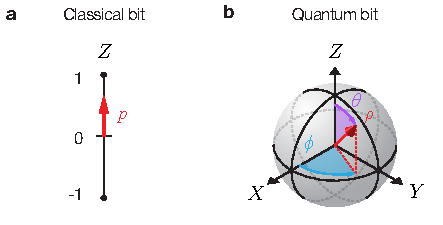
\includegraphics[scale=1.6]{mthry/BlochLineAndSphere}
\par\end{centering}
\caption[Geometric representation of the state of a classical and quantum bit]{\textbf{Geometric representation of the state of a classical and
quantum bit.} \textbf{\label{fig:Geometric-representation-of}a, }State
of a classical bit system represented as the one-dimensional probability
vector $p$ on the line segment Z between $-1$ and $1$ (see Eq.~(\ref{eq:ExpecL1})
for the definition of Z). \textbf{b, }State of quantum bit (qubit)
represented as the three-dimensional Bloch vector.  Unlike the classical
bit, the qubit has three observables (X, Y, and Z), which do not commute.
The quantum state of the qubit, $\rho$, is bounded by the unit sphere.
The surface of the sphere contains all pure states, which can be parametrized
by the angles $\phi$ and $\theta$. }
\end{figure}


\paragraph{\emph{Probabilistic bit system with perfect measurements.}}

For concreteness, consider a coin that is prepared probabilistically,
such as by a coin toss. Following the toss, an observer can perform
a measurement of the coin variable $S$, which yields a measurement
result. Formally, we should distinguish the measurement result obtained
by the observer from the actual value of the system property $S$.
For completeness, let's denote the variable of the \emph{measurement}
\emph{result} of $S$ as $m_{S}$. By analogy with $S$, we could
assign $m_{S}=-1$ and $m_{S}=1$ to results that corresponds to heads
and tails, respectively. The distinction between the measurement result
$m_{S}$ and system variable $S$ is crucial for imperfect and quantum
measurements. However, for simplicity, let us first proceed by assuming
perfect, classical measurements where there is no confusion between
$S$ and $m_{S}$, i.e, $m_{S}=S$. In this case, $m_{S}$ is redundant,
and for the following discussion there is no need to insist on the
distinction.

\emph{State of the system — a probability distribution.} To describe
the expected outcome of a measurement on the system, we introduce
the concept of the system \emph{state}.\footnote{For the following discussion, it suffices to adopt the point of view
that the state of the system represents \emph{subjective }knowledge
of the observer regarding the system. } The state describes the probability of a configuration to be the
system state. In other words, mathematically, the state is a probability
distribution over all possible system configurations, which form a
space known as the\emph{ configuration space}, denoted $\mathbb{S}$;
for the bit, $\mathbb{S}\equiv\left\{ S=1,S=-1\right\} $. The probability
for the coin be in the tails configuration, $S=1$, is then written
as $\Pr{S=1}$. More generally, the probability that the variable
$S$ of the system will have the value $s$ is $\Pr{S=s}$; for a
bit, $s\in\left\{ 1,-1\right\} $.\footnote{In this section, we employ the convention that capital letters denote
variables (typically, random ones) and lower case letters denote values.} This description of the classical system in terms of a probability
distribution, $\Pr{S=s}$, is analogous to the density matrix description
of a quantum system.\footnote{However, note that, as a probability, $\Pr{S=s}$ is a real and positive
number between 0 and 1.} Motivated by the analogy, we express the state of the coin bit as
a vector of probabilities, 
\begin{equation}
\vec{S}\equiv\begin{pmatrix}\Pr{S=1}\\
\Pr{S=-1}
\end{pmatrix}\,.\label{eq:SforBit}
\end{equation}
Keeping in mind the constraint that a measurement always yields a
result, one observes that the sum of the probabilities must be one.
Mathematically, the state vector $L^{1}$ norm is constrained, $\left|\vec{S}\right|_{\mathrm{L1}}=\sum_{s}\Pr{S=s}=1$,
where $\left|\cdot\right|_{\mathrm{L1}}$ denotes the $L^{1}$ norm.
This property is analogous to the unit-trace property of the density
matrix of a quantum state. Using this constrain, the state of the
coin, Eq.~(\ref{eq:SforBit}), can be simplified to a single information
parameter $p$, which denotes the bias of the coin,

\begin{equation}
\vec{S}=\begin{pmatrix}\frac{1+p}{2}\\
\frac{1-p}{2}
\end{pmatrix},\label{eq:BitBloch}
\end{equation}
The bias parameter $p$ is a number between $-1$ and 1,\footnote{Mathematically, $p$ is a number in the convex hull defined by $\mathbb{S}$.}
and, since it specifies the system state, is a quantity of central
importance. It can be viewed as the classical analog of the Bloch
vector of a quantum bit. In a sense, it represents a kind of one-dimensional
probability vector, which constitutes a geometric representation of
the system state; see Fig.~\ref{fig:Geometric-representation-of}a.

\paragraph{Operations on the system. }

An operation on the system results in a change of its configuration.
For the example of a coin, there are only two possible operations:
i) the coin is flipped (the logical negation operation, \emph{not})
or ii) the coin is left as is (the \emph{identity} operation). Working
within the framework of an ensemble of systems, an operation (one
that is applied to all systems in the ensemble) results in a change
of the state of the system that can be described by a linear map.
The state of the system ensemble after the operation, denoted $S'$,
can then be written as $\vec{S}'=U\vec{S}$, where the linear map
is represented by a configuration-transition matrix, denoted $U$.
For the coin, the two possible operations, the \emph{identity} and
\emph{not,} take the following forms
\begin{equation}
I\equiv\begin{pmatrix}1 & 0\\
0 & 1
\end{pmatrix}\text{\ and\ }\sigma_{x}\equiv\begin{pmatrix}0 & 1\\
1 & 0
\end{pmatrix}\,,\label{eq:IandSigmaX}
\end{equation}
respectively. The bit-flip Pauli matrix is denoted $\sigma_{x}$.


\paragraph{Perfect classical measurement of a system ensemble.}

Consider the long-run average value a series of repeated measurements
of the coin variable $S$, for the example of randomly prepared coins.
The expected mean value of $S$ is the weighted average of the results,
defined as
\begin{equation}
\E S\equiv\sum_{s}s\Pr{S=s}\,,\label{eq:EofS}
\end{equation}
where $\E{\cdot}$ represents ``expectation value of'' and the sum
is taken over all possible values $s$ of $S$. In matrix form, recalling
Eq.~(\ref{eq:BitBloch}), Eq.~(\ref{eq:EofS}) simplifies to

\begin{equation}
\E S=\left|\sigma_{Z}\vec{S}\right|_{\mathrm{L1}}=p\,,\label{eq:ExpecL1}
\end{equation}
where $p$ is non-negative and we have introduced the measurement
operator $\sigma_{Z}$, associated with the variable $S$ and given
by the Pauli matrix

\begin{equation}
\sigma_{Z}\equiv\begin{pmatrix}1 & 0\\
0 & -1
\end{pmatrix}\,.\label{eq:SigmaZ-CM}
\end{equation}
The matrix formulation given by Eq.~(\ref{eq:ExpecL1}) for the expectation
value of a classical measurement bears marked resemblance to that
employed with quantum systems. For a measurement on a quantum bit,
the expectation value of the $Z$ component of its spin is given by
$\Tr{\hat{\sigma}_{z}\rho}$, where $\rho$ is the qubit density matrix,
$\hat{\sigma}_{z}$ is the Pauli Z operator, represented by the matrix
given in Eq.~(\ref{eq:SigmaZ-CM}), and $\Tr{\cdot}$ denotes the
trace function. 

\begin{table}
\begin{centering}
\renewcommand*\arraystretch{1.5}
\begin{tabular}{l|c|>{\raggedright}p{0.5\columnwidth}}
\textbf{Concept} & \textbf{Symbols} & \textbf{Definition / Description}\tabularnewline
\hline 
\hline 
\multicolumn{3}{c}{\textbf{\rule{0pt}{5ex}Basic concepts}}\tabularnewline
\hline 
variable & $S$,$E$ & Describes intrinsic property of system, has definite value independent
of measurement apparatus\tabularnewline
\hline 
variable value & $s,e$ & Specific value that a variable can take\tabularnewline
\hline 
probability & $\Pr{S=s}$ & Probability that variable $S$ has value $s$\tabularnewline
\hline 
configuration & $\left\{ S\right\} $,$\left\{ E\right\} $,$\left\{ S,E\right\} $ & Set of all system variables\tabularnewline
\hline 
configuration space & $\mathbb{S}$,$\mathbb{E}$,$\mathbb{J}$ & Set of all possible system configurations\tabularnewline
\hline 
state  & $\vec{S},\vec{E},\vec{J}$ & Probability distribution on the configuration space, represented as
a vector\tabularnewline
\hline 
expectation value & $\E S$ & Expected (mean) value of repeated measurements of $S$, see Eq.~(\ref{eq:EofS})
\tabularnewline
\end{tabular}
\par\end{centering}
\caption[Basic concepts of classical measurement theory]{\textbf{Basic concepts of classical measurement theory.} }
\end{table}


\paragraph{Composite system. }

Extending the coin example, consider a composite system consisting
of two coins. The first coin is described by the variable $S$, or
in the ensemble situation, by the state $\vec{S}$, defined over the
configuration space $\mathbb{S}\equiv\left\{ S=1,S=-1\right\} $.
The second coin is similarly described by a single variable, $E$,
and a state $\vec{E}=\begin{pmatrix}\frac{1+p_{E}}{2}\\
\frac{1-p_{E}}{2}
\end{pmatrix}$, where $p_{E}$ is the coin bias. Its configuration space is $\mathbb{E}\equiv\left\{ E=1,E=-1\right\} $.
The configuration of the composite system consists of the simultaneous
specification of all variables, namely, $S$ and $E$. The set of
all possible configurations of the composite system is
\begin{align}
\mathbb{J} & =\mathbb{S}\otimes\mathbb{E}\label{eq:compsite-sys}\\
 & =\left\{ 1_{S},-1_{S}\right\} \otimes\left\{ 1_{E},-1_{E}\right\} \nonumber \\
 & =\left\{ 1_{S}1_{E},\,1_{S}-1_{E},\,-1_{S}1_{E},\,-1_{S}-1_{E}\right\} \,,\nonumber 
\end{align}
where $\otimes$ denotes the tensor product, and where, momentarily,
we have used the notation where $1_{S}$ stands for $S=1$.\footnote{So that no confusion arises, we note that the dimension of the composite
system space is not the sum but is the product of the subsystem dimensions,
i.e., $\dim\mathbb{J}=\dim\mathbb{S}\times\dim\mathbb{E}$, where
$\dim$ represents ``dimension of.''} The state of the composite system is a probability distribution over
$\mathbb{J}$, which can be represented by a 4-dimensional probability
vector, $\vec{J}$. When the two subsystems are uncorrelated, the
composite state is separable, and can be written as a simple product
of the states of the constituent subsystems, $\vec{J}=\vec{S}\otimes\vec{E}$.
However, when the subsystems are correlated, this is no longer possible.
For concreteness, consider the case where the two coins are prepared
randomly but always the same, the correlated randomness of the two
systems is described by the composite state  $\vec{J}=\left(\frac{1}{2},0,0,\frac{1}{2}\right)^{\intercal}$,
where $^{\intercal}$ denotes the transposition operation. More generally,
an operation that represents an interaction between the two coins
results in statistical correlations between them, and thus renders
the composite state inseparable. These features generally carry over
to the description of composite quantum systems, but standard statistical
correlations are replaced by entanglement. In the following subsection,
Sec.~\ref{subsec:Classical-model-of}, we explore the effect of an
interaction between the two coins.

\subsection{Classical toy model of system-environment interaction\label{subsec:Classical-model-of}}

For a more general discussion of measurements, it is necessary to
consider the interaction of the system with another, which probes
it and is often referred to as the \emph{environment}. In this subsection,
we consider the minimal limit of this model, where both the system
and environment are bits. Further, to introduce only the essentials
for now, we consider only the effect of a single interaction between
the classical system and environment, and discuss the effect of the
interaction on the system transfer of information. In the following
subsection, Sec.~\ref{subsec:Quantum-model-of}, we consider the
analogous quantum case, consisting of the interaction between a system
and environment, each of which is quantum bit. In Sec.~\ref{sec:Introductory-example:-qubit},
we generalize the toy model to the time-continuous homodyne monitoring
of a quantum bit. 

\begin{figure}
\begin{centering}
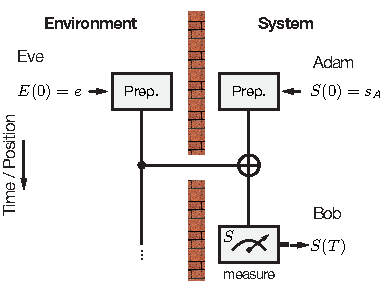
\includegraphics[scale=1.5]{mthry/SamAndEve}
\par\end{centering}
\caption[Classical toy model of the interaction between the system and environment]{\textbf{\label{fig:Reversibility-of-classical}Classical} \textbf{toy
model of the interaction between the system and environment.} Circuit
of the interaction between the system, with agents Adam and Bob, and
the environment, with agent Eve. Vertical lines depict the bits of
the system and environment, initially prepared by Adam and Eve in
the states $S\left(0\right)=s_{A}$ and $E\left(T\right)=e$, respectively.
The two bits interact via a controlled-NOT (cNOT) gate. Bob measures
the system at time $T$, obtaining the value $S\left(T\right)$. Brick
wall depicts the lack of communication between the agents of the system
and environment. }
\end{figure}


\paragraph{Classical toy model. }

Continuing with the example of two coins, we label one as the ``system''
and the other as the ``environment.'' For definitiveness, consider
the case where the system coin belongs to Adam, who aims to employ
it to communicate with Bob. To achieve this, at time $t=0$, Adam
prepares his coin in the configuration $S\left(0\right)=s_{A}$, where
$s_{A}$ is the bit value Adam hopes to communicate. He sends the
coin flying to Bob, who receives it at time $T$, and measures it
to obtain the value of $S\left(T\right)$. If the coin flies undisturbed,
$S\left(T\right)=S\left(0\right)$, and Bob faithfully receives Adam's
bit. 

However, during its flight, the coin unavoidably interacts with a
second flying coin, which belongs to an agent, Eve, who, at time $t=0$,
has prepared her coin in the configuration $E\left(0\right)=e$, where
$E$ is the variable describing her coin, and which is unknown to
Adam and Bob. For concreteness, suppose the interaction between the
two coins is described by the controlled-NOT (cNOT) gate, 
\begin{equation}
\mathrm{cNOT}\equiv I\otimes\begin{pmatrix}1 & 0\\
0 & 0
\end{pmatrix}+\sigma_{x}\otimes\begin{pmatrix}0 & 0\\
0 & 1
\end{pmatrix}=\begin{pmatrix}1 & 0 & 0 & 0\\
0 & 0 & 0 & 1\\
0 & 0 & 1 & 0\\
0 & 1 & 0 & 0
\end{pmatrix}\,,\label{eq:cNOT}
\end{equation}
where I and $\sigma_{x}$ are defined according to Eq.~(\ref{eq:IandSigmaX}).
Matrices associated with operations on the system (resp: environment)
are placed to the left (resp: right) of the tensor product. Given
that Adam and Bob lack knowledge of Eve's bit value, $e$, but are
aware of the interaction, to what degree can they communicate, i.e.,
what is the effect of the interaction on the value, $S\left(T\right)$,
measured by Bob?  More importantly, what action can Bob undertake
to undo the effect of the interaction, so as to obtain Adam's bit,
$S\left(T\right)=S\left(0\right)$? 

\paragraph{Evolution of the state, and Bob's information gain. }

Employing the formalism developed in Section~\ref{subsec:Classical-measurement-theory-basic-concept},
the initial state of the composite system, consisting of the two coins,
is described by the state vector $\vec{J}\left(0\right)=\vec{S}\left(0\right)\otimes\vec{E}\left(0\right),$
where the initial states of the system and environment are $\vec{S}\left(0\right)=\begin{pmatrix}\frac{1+s_{A}}{2}\\
\frac{1-s_{A}}{2}
\end{pmatrix}$ and $\vec{E}\left(0\right)=\begin{pmatrix}\frac{1+p_{E}}{2}\\
\frac{1-p_{E}}{2}
\end{pmatrix},$ respectively. The variable $p_{E}$ denotes the bias of Eve's coin,
see Eq.~(\ref{eq:BitBloch}). Following the interaction, the composite
system state is given by $\vec{J}\left(T\right)=\mathrm{cNOT\,}\vec{J}\left(0\right)$.
The expected mean value of Bob's measurement of $S\left(T\right)$,
represented by the matrix $I\otimes\sigma_{z}$, is given by, recalling
Eq.~(\ref{eq:ExpecL1}),
\begin{equation}
\E{S\left(T\right)}=\left|\left(I\otimes\sigma_{z}\right)\vec{J}\right|_{\mathrm{L1}}=p_{E}s_{A}.\label{eq:EsSamAdam}
\end{equation}
To understand Eq.~(\ref{eq:EsSamAdam}), consider three limiting
cases: i) Eve always prepares her coin facing up, $e=1$, corresponding
to a maximal coin bias, $p_{E}=1$. Since for $e=1$ the interaction
with her coin has no effect on Adam's coin, Bob faithfully receives
Adam's bit every time, $\E{S\left(T\right)}=s_{A}$. ii) Eve always
prepares her coin facing down, $e=-1$. Since her coin bias is now
$p_{E}=-1$, Bob always receives Adam's coin flipped $\E{S\left(T\right)}=-s_{A}$.
While inconvenient for Bob, by flipping each coin he receives (a deterministic
action), he could recover the bit. The effect of Eve's coin is to
change the encoding of the information, but has not resulted in its
loss. iii) Eve prepares her coin completely randomly, $p_{E}=0$.
On average, Bob receives no information from Adam, $\E{S\left(T\right)}=0$!
Eve has  randomly scrambled the encoding of the information for each
of the realizations, which, from Bob's point of view, results in the
complete loss of the initial system information encoded by Adam. More
generally, for an arbitrary coin bias $p_{E}$, the information shared
between Adam and Bob is characterized by the correlation between the
initial and final configurations of the system, which is given by
the bias of Eve's bit, $\E{S\left(T\right)S\left(0\right)}=p_{E}$,
which can be understood as the result of information transfer between
the system and environment, facilitated by the cNOT interaction, however,
where the ``information'' propagating to the system from the environment
is random noise. 

While the transfer of information between Adam and Bob is degraded
by the influence of the interaction with Eve's bit, in principle no
information has been erased, because the cNOT interaction is reversible.
For the case where $p_{E}=0$, Adams bit, $s_{A}$, is not transferred
to Bob at all; rather, it is encoded in the correlation between the
system and environment, $\E{S\left(T\right)E\left(T\right)}=\left|\left(\sigma_{z}\otimes\sigma_{z}\right)\vec{J}\right|_{\mathrm{L1}}=s_{A}$,
which is inaccessible to Adam and Bob, who only have control over
the system coin, and, hence, only access to $S$. To summarize, the
interaction between the system and a randomly prepared random environment
results in loss of information and injection of noise into the system,
as far as the system alone is concerned. Nevertheless, from the vantage
point of the composite system, no information is lost; rather, it
is transferred into correlations between the system and environment. 

\paragraph{Recovering the information.}

To recover Adam's bit, Bob requires access to Eve's physical coin
or knowledge of $e$, the specific value of her coin for \emph{each}
realization. First, consider the latter case, where Bob learns $e$.
Recalling that $\mathrm{cNOT}^{2}=I\otimes I$, before Bob performs
a measurement, he can undo the interaction effect by preparing an
ancillary, third, coin with the value $e$, by employing it to perform
a second cNOT operation on his coin, thus reversing the first. Applied
to each realization, this procedure results in faithful communication,
$\E{S\left(T\right)S\left(0\right)}=1$. Notably, Bob can also reverse
the interaction effect\emph{ after} performing his measurement by
essentially applying the second cNOT operation virtually, i.e., when
$e=1$, $s_{A}=s_{B}$, while otherwise, $s_{A}=-s_{B}$. We remark
that any operations performed by Eve on her coin after the system-environment
interaction have no consequences for Bob. To summarize, the examples
highlights three distinct aspects regarding the recovery of information
in the classical setting:
\begin{enumerate}
\item Eve's physical system was not required, only information about its
initial configuration, $E\left(0\right)=e$.
\item The effect of the interaction can be reversed \emph{before} or \emph{after}
Bob's measurement. 
\item Operations on Eve's coin subsequent to the interaction have no consequences.
\end{enumerate}
All three of these features break down in the quantum setting, as
discussed in the following subsection. 

\subsection{Quantum toy model\label{subsec:Quantum-model-of}}

Rather than communicating with classical bits (coins), consider the
situation where Adam and Bob communicate with quantum bits (qubits),
and Eve too employs a qubit. Before proceeding, we briefly review
the basic qubit concepts.

\paragraph{Quantum bit. }

While the fundamental concept of classical information is the bit,
which represents the minimal classical system, the fundamental concept
of quantum information is the \emph{quantum bit}, or \emph{qubit}
for short, which represents the minimal physical quantum system. A
qubit has two basis states, $\ket{+z}$ and $\ket{-z}$. A pure state
of the qubit  is described by the state $\ket{\psi}=\cos\left(\frac{\theta}{2}\right)\ket{+z}+e^{i\phi}\sin\left(\frac{\theta}{2}\right)\ket{+z}$,
where the angles $\theta$ and $\phi$, which fall in the range $0\leq\theta\leq\pi$
and $0\leq\phi\leq2\pi$, define a point on the unit sphere, known
as the \emph{Bloch sphere}, see Fig.~\ref{fig:Geometric-representation-of}b.
 More generally, a statistical ensemble of pure states, a \emph{mixed}
qubit state is described by the density matrix 
\begin{equation}
\rho=\frac{1}{2}\left(\hat{I}+X\hat{\sigma}_{x}+Y\hat{\sigma}_{y}+Z\hat{\sigma}_{z}\right)\,,
\end{equation}
where $X$, $Y$, $Z$ are real numbers parameterizing the state,
given by the averages of the Pauli operators, $X\equiv\Tr{\hat{\sigma}_{x}\rho}$,
\emph{et cetera}, where $\Tr{\cdot}$ denotes the trace operation.
The matrix representation of the identity, $\hat{I}$, and Pauli $\hat{\sigma}_{x}$
and $\hat{\sigma}_{z}$ operators is given in Eqs.~(\ref{eq:IandSigmaX})
and (\ref{eq:SigmaZ-CM}), while that of Pauli operator Y is $\hat{\sigma}_{y}=\begin{pmatrix}0 & -i\\
i & 0
\end{pmatrix}$, where $i$ is the unit imaginary. The Bloch vector, $\left(X,Y,Z\right)^{\intercal}$,
provides an important geometrical representation of the state of the
qubit, and as discussed in Sec.~\ref{subsec:Classical-measurement-theory-basic-concept}
is the analog of the coin bias $p$. For a pure state, the Bloch vector
extends to the surface of the Bloch sphere, while for mixed states,
it lies in the interior. Notably, it admits the spherical parameterization:
\begin{align}
X & =r\sin\left(\theta\right)\cos\left(\phi\right)\,,\nonumber \\
Y & =r\sin\left(\theta\right)\sin\left(\phi\right)\,,\nonumber \\
Z & =r\cos\left(\theta\right)\,,\label{eq:XYZBLoch}
\end{align}
where the angles $\theta$ and $\phi$ are defined as for pure states
and $r$ is the length of the Bloch vector, a number between 0 and
1. Notably, in the Bloch representation, mutually orthogonal state
vectors are \emph{not} represented by orthogonal Bloch vectors, but
rather, by opposite Bloch vectors, which specify antipodal points
on the sphere. 

\paragraph{Quantum toy model. }

Returning to the toy model example of the interaction between two
systems (recall Fig.~\ref{fig:Reversibility-of-classical}, which
depicts the analogous classical model), we consider the case where
at time $t=0$ Adam prepares his qubit in the pure state $\ket{\psi\left(0\right)}$,
with corresponding Bloch vector components $X\left(0\right)$, $Y\left(0\right)$,
and $Z\left(0\right)$, while Eve prepares her qubit in the pure state
$\ket{+x}$, where $\ket{+x}=\frac{1}{\sqrt{2}}\left(\ket{+z}+\ket{+z}\right)$.
Unlike in the classical toy model, Adam has a choice regarding the
encoding of his information — the orientation of the Bloch vector,
which has no classical analog. Both qubits are sent flying. A controlled-NOT
interaction occurs, described by the operator $\mathrm{cNOT}=\hat{I}\otimes\kb{+z}{+z}+\hat{\sigma}_{x}\otimes\kb{-z}{-z}$,
where operators on the left (resp., right) of the tensor product,
denoted $\otimes$, act on the system (resp., environment). Notably,
the matrix representation of the cNOT operator is the same that of
the classical cNOT gate, given in Eq.~(\ref{eq:cNOT}). After the
interaction Bob receives the system qubit, at time $T$. 

\paragraph{Effect of the interaction before the measurement. }

Before the measurement, the pure state of the composite system, $\ket{\Psi\left(T\right)}=\mathrm{cNOT}\left(\ket{\psi\left(0\right)}\ket{+x}\right)$,
is, in general, inseparable — it cannot be written as a simple product
of states of its component systems. On a mathematical level, this
result is the same as that for the classical model; however, the interpretation
and consequences are markedly distinct. Classically, the inseparability
represented statistical correlations between \emph{definite} configurations
of the system and environment. For the quantum model, the inseparability
represents entanglement between the system and environment — the system
cannot be fully described without considering the environment. Generally,
measurements of the entangled system are correlated with those of
the environment, and the system alone cannot be represented by a pure
state. The consequences of the system-environment entanglement are
at the heart of quantum measurement theory. 

Consider the reduced density matrix of the system qubit, found by
taking the partial trace over the environment, denoted $\mathrm{Tr}_{E}\left[\cdot\right]$,
\begin{equation}
\rho_{S}\left(T\right)=\mathrm{Tr}_{E}\left[\ketbra{\Psi\left(T\right)}{\Psi\left(T\right)}\right]=\frac{1}{2}\begin{pmatrix}1 & X\left(0\right)\\
X\left(0\right) & 1
\end{pmatrix}\,.\label{eq:rho_s-env-q}
\end{equation}
Evidently, entanglement in the composite state, the result of the
interaction between the system and environment results in the loss
of information from the point of view of the system. Specifically,
the $Y$ and $Z$ Bloch components prepared by Adam, $Y\left(0\right)$
and $Z\left(0\right)$, are absent in $\rho_{S}\left(T\right)$, despite
the deterministic preparation of the ancilla in a\emph{ pure} state
$\ket{+x}$. However, if Adam chose to encode his information along
the X component of the Bloch vector, it would propagate to Bob undisturbed
by the interaction with the environment, and Bob could receive it
by measuring $X$. It is the $X$ component that is preserved due
to the choice of the interaction and initial pure state of the environment.
Analogously to the classical case, no information is truly lost, but
rather, when viewed in the broader context of the composite system,
Adam's initial $Y$ and $Z$ qubit components are encoded in the YZ,
$\left\langle YZ\right\rangle \equiv\Tr{\left(\hat{\sigma}_{y}\otimes\hat{\sigma}_{z}\right)\rho}=Y\left(0\right)$,
and ZZ, $\left\langle ZZ\right\rangle \equiv\Tr{\left(\hat{\sigma}_{z}\otimes\hat{\sigma}_{z}\right)\rho}=Z\left(0\right)$,
correlations between the system and environment, respectively.


\paragraph{Recovering information before the measurement. }

In the classical case, by learning the initial configuration of the
environment, $E\left(0\right)=e$, Bob could undo the effect of the
system-environment interaction and could recover the state sent by
Adam before performing the measurement. In the quantum case, this
is not possible. Even though Bob can know the initial state, $\ket{+x}$,
of the environment and can clone it, by preparing a third ancilla
qubit in the state $\ket{+x}$, he cannot use this ancilla to perform
a second cNOT operation on the system so as to reverse (recall that
$\mathrm{cNOT}^{2}=\hat{I}$) the cNOT performed by the environment
qubit. This is a profound consequence of the entanglement between
the system and environment, and has no classical analog. The only
way to reverse the interaction is to use the physical qubit of the
environment to perform the second cNOT operation — \emph{no} clone
will suffice. 

\paragraph{Projective (von Neumann) measurement.\label{par:Projective-(von-Neumann)}}

For a classical system described by a state of maximal knowledge,
the result of any measurement can be determined with certainty. However,
for a quantum system described by a state of maximal knowledge, a
pure state, the result of a measurement is \emph{not}, in general,
determined. For definitiveness, consider the description of a perfect
projective (von Neumann) measurement performed by Bob on the $Z$
component of his qubit spin, with the associated  operator (\emph{observable})
$\hat{\sigma}_{z}$.  The measurement is described by the spectral
decomposition of the observable, $\hat{\sigma}_{z}=\sum_{r}r\hat{\pi}_{r}=\hat{\pi}_{1}-\hat{\pi}_{-1}$,
where $r$ is an eigenvalue, $r=1$ or $r=-1$, to which corresponds
a measurement result, and $\hat{\pi}_{r}$ is the projection operator
onto the eigenstate associated with $r$, $\hat{\pi}_{1}=\kb{+z}{+z}$
and $\hat{\pi}_{-1}=\kb{+z}{+z}$. The probability of obtaining an
outcome corresponding to the eigenvalue $r$ is
\begin{equation}
\wp_{r}=\Tr{\hat{\pi}_{r}\rho}\,.\label{eq:ProbOfprojMsr}
\end{equation}
According to the projection postulate of quantum mechanics,\footnote{Curiously, the modern formulation of the projection postulate is not
precisely that of von Neumann \citep{VonNeumann1932}, but contains
a correction due to Lüders \citep{Luders1951}. } the measurement leads to the projection (or ``collapse'')\footnote{W. Heisenberg introduced the idea of wavefunction collapse in 1927
\citep{Heisenberg1927}.} of the system state into an eigenstate of the measurement operator.
Immediately after the measurement, conditioned on the result $r$,
the state of the system is 
\begin{equation}
\rho_{r}=\frac{\hat{\pi}_{r}\rho\hat{\pi}_{r}}{\wp_{r}}\,.\label{eq:projectionPostulate}
\end{equation}
The evolution due to Eq.~(\ref{eq:projectionPostulate}) is markedly
non-linear in the state density, which appears in the denominator,
and represents a radical departure from the linear evolution encountered
with Schrödinger’s equation. Further, while a perfect measurement
of a classical system does \emph{not} alter its state, a perfect measurement
of a quantum system, in general, \emph{does} alter its state. This
non-linear disturbance has profound consequences.

Suppose, at time $T$, Bob performs a $Z$ measurement of his qubit
and obtains the result $r=1$, with probability, recalling Eqs.~(\ref{eq:rho_s-env-q})
and~(\ref{eq:ProbOfprojMsr}), $\wp_{1}=\Tr{\hat{\pi}_{1}\rho_{S}\left(T\right)}=\frac{1}{2}$.
Note that $\wp_{1}$ is independent of $X\left(0\right)$, $Y\left(0\right)$,
and $Z\left(0\right)$. The system state after the measurement is
$\rho_{1}=\hat{\pi}_{1}\rho_{S}\left(T\right)\hat{\pi}_{1}/\Tr{\rho_{S}\left(T\right)\hat{\pi}_{1}}=\begin{pmatrix}1 & 0\\
0 & 0
\end{pmatrix}$, corresponding to the pure state $\ket{+z}$. Notably, the potentially
recoverable information encoded by Adam, $X(0)$, is irreversibly
lost. From the point of view of the composite system, described by
the state $\ket{\Psi\left(T\right)}$, the measurement has projected
the state onto the measurement basis, according to the effect of the
projector $\hat{\pi}_{1}\otimes\hat{I}$. The state of the composite
system after the measurement, $\ket{+z}\ket{\psi\left(0\right)}$,
is pure and separable, i.e., the measurement has disentangled the
system and environment. In this toy model (and for this particular
measurement outcome), it just so happens that Adam's state is completely
teleported to Eve's qubit, a form of information transfer between
the two systems. To understand the situation a bit better, consider
the alternative, where $r=-1$, with the associated projector $\hat{\pi}_{-1}\otimes\hat{I}$.
The conditional state of the system after the measurement is again
obtained by employing Eq.~(\ref{eq:projectionPostulate}), yielding
$\ket{+z}\ket{\psi'}$ for the composite system, where the state $\ket{\psi'}$
has the same Bloch vector as Adam's initial state $\ket{\psi\left(0\right)}$
but with the $Y$ and $Z$ components flipped. This example illustrates
the more general feature that a measurement on either the system or
environment disentangles the two, resulting in a perfect correlation
between the measurement on one and the state of the other. Further,
it tends to lead to a transfer of information between the two subsystems.
We explore the profound consequences of these features in the following
section.


\section{Continuous Quantum Measurements: Introduction to Quantum Trajectories
and Stochastic Calculus \label{sec:Introductory-example:-qubit} }
\sectionmark{Continuous Quantum Measurements}

In this section, we consider a heuristic microscopic model of continuous
quantum measurements, which, although simple, contains sufficient
generality to introduce the principal ideas. Specifically, we model
the homodyne measurement of a qubit by a sequence of interactions
with a chain of identically prepared ancilla qubits.  A chain of
ancillary systems modeling the environment is known as a von Neumann
chain \citep{VonNeumann1932}. While the evolution due to the interaction
with each ancilla is unitary, ``deterministic,'' the addition of
a projective (von Neumann) measurement of each ancilla subsequent
to its interaction with the system results in the stochastic evolution
of the quantum state of the system — known as a\emph{ quantum trajectory}
\citep{Carmichael1993}. Due to the correlation between the state
of a measured ancilla and the resulting  state of the system, the
measurement results allow faithful tracking of the state trajectory
\citep{belavkin1987non,Carmichael1993,Gardiner1992-original-traj,Dalibard1992-original-traj,Korotkov1999-original-traj}.
After introducing the time-discrete version of the model, we take
its continuum limit, which allows us to introduce the fundamental
concepts of stochastic calculus. Specifically, we focus on introducing
the Wiener noise process and obtaining the stochastic differential
equations (SDEs) that describe the homodyne monitoring of the qubit.
Most of the results derived in this section carry over with little
modification to the following section, Sec.~\ref{sec:Quantum-trajectory-theory},
which establishes the general formulation of quantum measurement theory.
Time-discrete chain models have been discussed in Refs.~\citet{Caves1987-time-discrete,Attal2006,Tilloy2015,Korotkov2016-qm-bayes,Bardet2017}.

 

\subsection{Time-discrete model with flying spins}

\begin{figure}
\begin{centering}
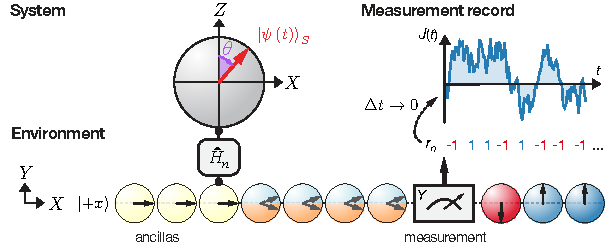
\includegraphics[scale=1.4]{mthry/SpinBathModelFigure}
\par\end{centering}
\caption[Homodyne monitoring of a quantum bit: time-discrete model]{\textbf{\label{fig:Ch2:SpinBathModel1}Homodyne monitoring of a quantum
bit: time-discrete model.} The qubit, whose Bloch vector lies in the
XZ plane, sequentially interacts with a chain of ancilla qubits, which
model the environment. At the beginning of each timestep, at time
$t$, the system is in a pure state, $\ket{\psi\left(t\right)}_{S}$.
During the $n$-th timestep, of length $\Delta t$, the qubit interacts,
subject to the Hamiltonian $\hat{H}_{n}$, with the $n$-th ancilla,
prepared in $\ket{+x}$, whereafter, the Y component of its spin is
projectively measured. The result of the measurement, $r_{n}$, which
is either -1 or 1, is recorded and accumulated; in the continuum limit,
$\Delta t\rightarrow0$, it leads to the homodyne signal $J\left(t\right)$,
a time-continuous stochastic (Weiner) process.}
\end{figure}

Time is discretized in small but finite bins of length $\Delta t$
labeled by the integer $n$, i.e.,~$t=n\Delta t$. During each timestep,
a single spin of the environment, referred to as the \emph{ancilla},
interacts with the system for time $\Delta t$, see Fig.~\ref{fig:Ch2:SpinBathModel1}.
For simplicity, assume each spin is identically prepared in the state
$\ket{+x}$. We employ the convention that the states $\ket{\pm x}$,
$\ket{\pm y}$, and $\ket{\pm z}$ denote eigenstates of the Pauli
X, Y, and Z operators, respectively. The interaction between the $n$-th
ancilla and the system is described by the Hamiltonian 
\begin{equation}
\hat{H}_{n}\equiv-\frac{\hbar\lambda}{2}\hat{\sigma}_{z}^{S}\otimes\hat{\sigma}_{z}^{\left(n\right)}\,,
\end{equation}
where $\lambda$ is the strength of the interaction, $\hbar$ is Plank's
constant, and $\hat{\sigma}_{z}^{S}$ and $\hat{\sigma}_{z}^{\left(n\right)}$
denote the Pauli Z operators of the system and ancilla, respectively.
For the time being, we assume that $\hat{H}_{n}$ is the only generator
of system evolution, and the system Hamiltonian is zero, $\hat{H}_{S}=0$.
Following the interaction, the ancilla is measured by a detector that
performs a projective measurement of the ancilla spin  Y component,
which yields the measurement result $r_{n}=-1$ or $r_{n}=1$. The
observer operating the measurement apparatus keeps track of the sum
total of the measurement results, the measurement signal: $J_{t}\equiv\sqrt{\Delta t}\sum_{n'=0}^{n}r_{n'}$. 

Note two assumptions  regarding the measurement: i) the ancilla qubits
are undisturbed during their flight from the system to the measurement
apparatus, and ii) the measurement apparatus performs a perfect measurement,
and does not add technical noise. These assumptions ensure no information
is lost in the measurement, nor spurious noise is added by it; i.e.,
the observer has perfect access to all information there is to know
in the environment, and is hence referred to as an \emph{omniscient}
\emph{observer}. 

\subparagraph{Evolution of the composite system. }

For simplicity, assume the state of the system at time $t$ is pure
and its Bloch vector lies in the XZ plane; i.e., it is described by
a single angle $\theta\left(t\right)$, 
\begin{align}
\ket{\psi\left(t\right)}_{S} & =\cos\left(\frac{\theta\left(t\right)}{2}\right)\ket{+z}_{S}+\sin\left(\frac{\theta\left(t\right)}{2}\right)\ket{-z}_{S}=\begin{pmatrix}\cos\left(\frac{\theta\left(t\right)}{2}\right)\\
\sin\left(\frac{\theta\left(t\right)}{2}\right)
\end{pmatrix}\,.\label{eq:SpinBath:sysState}
\end{align}
The state of the composite system at time $t$, consisting of the
$n$-th ancilla and the system qubit, is $\ket{\Psi\left(t\right)}=\ket{\psi\left(t\right)}_{S}\otimes\ket{+x}_{n}$,
and for duration $\Delta t$ evolves subject to the Hamiltonian $\hat{H}_{n}$.
The total evolution is given by the propagator $\hat{U}\left(t,t+\Delta t\right)=\exp\left(-i\hat{H}_{n}\Delta t/\hbar\right)$,
and the composite-system state after the interaction is 
\begin{equation}
\ket{\Psi\left(t+\Delta t\right)}=\hat{U}\left(t,t+\Delta t\right)\ket{\Psi\left(t\right)}\,,
\end{equation}
Anticipating the ancilla Y measurement, we express $\ket{\Psi\left(t+\Delta t\right)}$
in terms of the measurement operator eigenstates. The measurement
operator on the ancilla alone is the Pauli Y operator, $\hat{\sigma}_{y}^{\left(n\right)}$,
with eigenstates $\ket{-y}_{n}$ and $\ket{+y}_{n}$, in terms of
which, 
\begin{equation}
\ket{\Psi\left(t+\dt\right)}=\ket{\tilde{\psi}_{-1}\left(t+\Delta t\right)}_{S}\otimes\ket{-y}_{n}+\ket{\tilde{\psi}_{+1}\left(t+\Delta t\right)}_{S}\otimes\ket{+y}_{n}\,,\label{eq:PsiQubitEnvSpin}
\end{equation}
where the parameter $\epsilon\equiv\lambda\Delta t$ characterizes
the measurement strength and the un-normalized\footnote{By convention, a tilde will indicate an unnormalized state, with a
norm less than one.} system states $\ket{\tilde{\psi}_{\pm1}\left(t+\Delta t\right)}_{S}$
are
\begin{equation}
\ket{\tilde{\psi}_{\pm1}\left(t+\Delta t\right)}_{S}\equiv\begin{pmatrix}\cos\left(\frac{\theta\left(t\right)}{2}\right)\cos\left(\frac{\pi/2\pm\epsilon}{2}\right)\\
\sin\left(\frac{\theta\left(t\right)}{2}\right)\sin\left(\frac{\pi/2\pm\epsilon}{2}\right)
\end{pmatrix}_{S}\,.\label{eq:SpinBath:psiTilde}
\end{equation}
The state of the composite system following the interaction, Eq.~(\ref{eq:PsiQubitEnvSpin}),
is not separable. The interaction has entangled the system and environment,
as discussed of Sec.~\ref{subsec:Quantum-model-of}.

\paragraph{Projective (von Neumann) measurement of the ancilla. }

The action of the measurement apparatus on the composite system is
described, recalling the discussion on Pg.~\pageref{par:Projective-(von-Neumann)},
by decomposing the measurement operator $\hat{Y}_{n}=\hat{I}\otimes\hat{\sigma}_{y}$
in terms of its  eigenstate projectors, $\hat{\pi}_{\pm}\equiv\hat{I}_{S}\otimes\left(\kb{\pm y}{\pm y}\right)_{n}$;
note, $\hat{Y}=\hat{\pi}_{+}-\hat{\pi}_{-}$. According to the von~Neumann
postulate, the projectors yield the probability for obtaining the
results $r_{n}=-1$ and $r_{n}=1$ from the measurement, 
\begin{align}
\wp_{r}\left(t\right) & =\bra{\Psi\left(t+\Delta t\right)}\hat{\pi}_{r}\ket{\Psi\left(t+\Delta t\right)}\nonumber \\
 & =\braket{\tilde{\psi}_{r}\left(t+\Delta t\right)}{\tilde{\psi}_{r}\left(t+\Delta t\right)}\nonumber \\
 & =\frac{1}{2}\left(1-r_{n}\sin\left(\epsilon\right)\cos\left(\theta\left(t\right)\right)\right)\,,\label{eq:PflyingSpinPM1}
\end{align}
as well as the state of the composite system immediately after the
measurement, conditioned on the result $r_{n}$, 
\begin{equation}
\ket{\Psi_{r}\left(t+\Delta t\right)}=\ket{\tilde{\psi}_{r}\left(t+\Delta t\right)}_{S}\ket{y:=r}_{n}/\sqrt{\wp_{r}\left(t\right)},\label{eq:Psir_afterMsr}
\end{equation}
where $\ket{y:=r}_{n}$ denotes ancilla state $\ket{+y}_{n}$ (resp.,
$\ket{-y}_{n}$) for $r=1$ (resp., $r=-1$). The measurement has
transformed the entanglement between the system and environment, evident
in the non-separable state $\ket{\Psi\left(t+\Delta t\right)}$, Eq.~(\ref{eq:PsiQubitEnvSpin}),
into a correlation between the pure state of the system and environment
after the measurement, evident in the separable, non-entangled conditional
state $\ket{\Psi_{r}\left(t+\Delta t\right)}$, Eq.~(\ref{eq:Psir_afterMsr}).
Assuming the ancilla never interacts with the system again, it is
unnecessary to retain it in the description of the measurement; removing
it from Eq.~(\ref{eq:Psir_afterMsr}), we obtain the pure state of
the system alone at time $t+\Delta t$:
\begin{align}
\ket{\psi_{r}\left(t+\Delta t\right)}_{S} & =\frac{1}{\sqrt{\wp_{r}\left(t\right)}}\ket{\tilde{\psi}_{r}\left(t+\Delta t\right)}_{S}=\begin{pmatrix}\cos\left(\frac{\theta_{r}\left(t+\dt\right)}{2}\right)\\
\sin\left(\frac{\theta_{r}\left(t+\dt\right)}{2}\right)
\end{pmatrix}\,.\label{eq:SpinModel:postState}
\end{align}
From the point of view of the observer, the entanglement is transformed
by the measurement into a classical correlation between the result
$r_{n}$ and the final conditional state of the system, $\ket{\psi_{r}\left(t+\Delta t\right)}_{S}$.
Figure~\ref{fig:Ch2:SpinBath} summarizes the steps of the model
and the conditional state update.

\begin{figure}
\begin{centering}
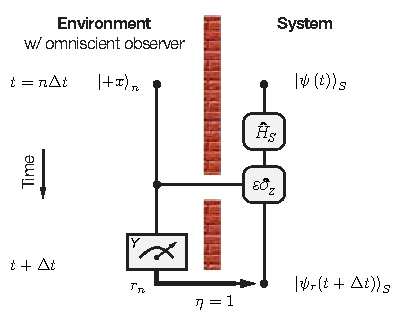
\includegraphics[scale=1.4]{mthry/SpinBathModel}
\par\end{centering}
\caption[Circuit representation of the $n$-th timestep of the quantum trajectory]{\textbf{\label{fig:Ch2:SpinBath}Circuit representation of the $n$-th
timestep of the quantum trajectory. }At time $t=n\Delta t$, the system,
described by the state $\ket{\psi\left(t\right)}_{S}$, is subjected
to the system Hamiltonian $\hat{H}_{S}$ and the interaction with
the $n$-th ancilla, characterized by the parameter $\epsilon$. Every
ancilla is prepared in $\ket{+x}$. Following the interaction, the
detector projectively measures the Y component of the ancilla spin,
yielding the result $r_{n}$, which provides the information necessary
to update the state of the system. In the case of the omniscient observer,
characterized by unit quantum measurement efficiency, $\eta=1$, at
the end of the timestep, immediately after $t+\Delta$, the system
state, $\ket{\psi_{r}\left(t+\Delta t\right)}_{S}$, conditioned on
the measurement result is pure. Contrast with Fig.~\ref{fig:Reversibility-of-classical}. }
\end{figure}


\paragraph{Solution for the conditional state update. }

To explicitly solve Eq.~(\ref{eq:SpinModel:postState}) for the updated
angle of the qubit system conditioned on the measurement result $r_{n}$,
$\theta_{r}\left(t+\Delta t\right)$, one can use Eqs.~(\ref{eq:PflyingSpinPM1})
and~(\ref{eq:SpinBath:psiTilde}), following trigonometric manipulation,
to obtain, without any approximations, an explicit relation (\citeauthor{MHD})
between the Bloch angle at the start and end of the timestep: 
\begin{equation}
\boxed{\tan\left(\frac{\theta_{r}\left(t+\Delta t\right)}{2}\right)=\tan\left(\frac{\theta\left(t\right)}{2}\right)\tan\left(\frac{\pi/2+r_{n}\epsilon}{2}\right)\,.}\label{eq:SpinBath:Ch2:tan}
\end{equation}
In the following section, Sec.~\ref{subsec:Random-walk-on}, this
seemingly non-linear equation is transformed into a linear equation
by a hyperbolic transformation of the circular angle $\theta$, and
is solved exactly. Nonetheless, for the continuum-limit discussion
in Sec.~\ref{subsec:Continuous-limit:-Wiener}, consider the solution
of Eq.~(\ref{eq:SpinBath:Ch2:tan}) in the limit of weak interactions,
$\epsilon\ll1$, to order $\epsilon$: 
\begin{equation}
\mathrm{d}\theta\left(t\right)\equiv\theta\left(t+\Delta t\right)-\theta\left(t\right)\approx\epsilon r_{n}X\left(t\right)\,,\label{eq:SPinBath:ThPM}
\end{equation}
where we have defined the Bloch angle increment, $\mathrm{d}\theta\left(t\right)$,
and $X\left(t\right)$ is the X component of the Bloch vector, $X\left(t\right)=\sin\left(\theta\left(t\right)\right)$. 

\paragraph{Interpretation and remarks. }

The system measurement dynamics are described in entirety by Eqs.~(\ref{eq:PflyingSpinPM1}),~(\ref{eq:SpinModel:postState}),
and~(\ref{eq:SPinBath:ThPM}). To make the discussion more concrete,
consider the particular case where the system and ancilla do not interact,
$\epsilon=0$. The measurement results are completely random, $\wp_{r}=\frac{1}{2}$,
uncorrelated with the system; similarly, the system state is independent
of the measurement results, $r_{n}$; in fact, there is no state evolution,
$\mathrm{d}\theta\left(t\right)=0$. Consider the more interesting
case of weak interactions, $\epsilon\ll1$. Measurement results are
correlated with the Z component of the system Bloch vector, $\wp_{r}=\frac{1}{2}\left(1-\epsilon r_{n}Z\left(t\right)\right)$,
where $Z\left(t\right)=\cos\left(\theta\left(t\right)\right)$. Nonetheless,
 due to $\epsilon\ll1$, the two measurement results still occur with
nearly equal probability, and the record consists of random noise,
but with a slight bias that correlates it with $Z$. Thus, the value
of $Z$ can be obtained from the instantaneous average of the measurement
results, $\E{r_{n}}=-\epsilon Z$. In time, from the point of view
of the observer, a long sequence of measurements gradually results
in the complete measurement of $Z$, obtained from the noisy measurement
record. A peculiar feature of the weak interaction regime, $\epsilon\ll1$,
is that amplitude of the noise is essentially constant for all measurement
strengths, its variance is $\mathrm{Var}\left[r_{n}\right]=1-\left(\epsilon Z\right)^{2}\approx1$.
This origin of the randomness can be interpreted to be quantum in
nature, since the system and environment are in pure states at all
times. Specifically, it is due to the incompatibility (orthogonality)
between the initial state of the ancilla, $\ket{+x}_{n}$, and the
eigenstates, $\ket{\pm y}_{n}$, of the measurement observable. 

The random measurement result, $r_{n}$, is correlated with a small
``kick'' on the state of the system, described by Eq.~(\ref{eq:SPinBath:ThPM}).
Conditioned on the result $r_{n}=1$ (resp., $r_{n}=-1$) the system
experiences a downward (resp., upward) kick corresponding to the circular
increment $\mathrm{d}\theta\left(t\right)=\epsilon r_{n}\mathrm{sgn}\left(X\left(t\right)\right)\sqrt{1-Z\left(t\right)}$,
whose magnitude is largest for $Z=0$, but vanishing in the limit
where $Z$ approaches $\pm1$; the sign function is denoted $\mathrm{sgn}$.
This state-dependent nature of the back-action kicks leads to the
eventual projection of the state onto one of the eigenstate of the
system observable, $\hat{\sigma}_{z}$, as discussed in Sec.~\ref{subsec:Random-walk-on}. 

The form of the backaction depends on the ancilla quantity being measured
by the apparatus; for example, a measurement of a quadrature other
than the ancilla $Y$ quadrature yields a different form of the measurement
backaction. More generally, we emphasize that no matter what ancilla
quantity is measured, so long as the measurement is projective and
complete knowledge about the ancilla is obtained, the ancilla is collapsed
onto a single unique state. From this, it follows that the system
cannot be entangled with the ancilla and for this reason the system
is left in a pure state. 

\paragraph{Generalized measurements. }

By introducing an ancilla that interacts unitarily with the system
and is subsequently measured, we obtained evolution equations for
the pure state of the quantum system conditioned on the measurement
result $r_{n}$, and could otherwise disregard the ancilla in the
measurement description. The ancilla scheme realizes an indirect measurement
of the system, which gradually obtains information about the system
and disturbs it in a manner that is indescribable with the von Neumann
formulation, summarized by Eqs.~(\ref{eq:ProbOfprojMsr}) and (\ref{eq:projectionPostulate}).
The example of this section belongs to a more general class of measurements,
referred to as \emph{generalized measurements}. A powerful theorem
by Neumark, see Sec.~9-6 of Ref.~\citet{PeresBook}, proved that
any generalized measurement can be formulated essentially according
to the scheme presented so far, where an auxiliary quantum system
is introduced, it interacts unitarily with the system, and is subsequently
projectively measured, in the traditional von~Neumann sense. The
effect of the generalized measurement on the system can be completely
described by system operators, denoted $\hat{M}_{r}$, that are not
in general Hermitian. For our example, the \emph{measurement operator,}\footnote{The measurement operator is sometimes referred to as a Kraus operator.}\emph{
$\hat{M}_{r}$,} follows directly from Eq.~(\ref{eq:Psir_afterMsr}),
\begin{equation}
\hat{M}_{r}\left(t\right)=\prescript{}{n}{\braOket{y:=r}{\hat{U}\left(t,t+\Delta t\right)}{+x}_{n}}\label{eq:MrSpinBath}
\end{equation}
Note that $\ket{+x}_{n}$ is the \emph{initial} ancilla state for
the $n$-th timestep, while $\ket{y:=r}_{n}$ is the \emph{final}
ancilla state, follwing the projective measurement, while $\hat{U}$
is the \emph{composite} system propagator. Since $\hat{M}_{r}$ in
Eq.~(\ref{eq:MrSpinBath}) is not\emph{ }Hermitian, it does not belong
to the traditional notion of an 'observable', and the outcomes $r_{n}$
are not the eigenvalues of $\hat{M}_{r}$, but serve merely as labels.
The measurement operators $\hat{M}_{1}$ and $\hat{M}_{-1}$, which
are non-orthogonal ($\hat{M}_{1}\hat{M}_{-1}\neq0$) link the system
state with the set of measurement probabilities $\wp_{r}$, and formally,
their operator set, $\left\{ \hat{M}_{r}^{\dagger}\hat{M}_{r}:r\right\} $,
constitutes a \emph{positive-operator-valued measure} (POVM) on the
space of results, see Sec.~2.2.6 of Ref.~\citet{NielsenChuangBook}.
In general, the measurement operators generalize von Neumann's postulate
in the following way:
\begin{align}
\wp_{r}\left(t\right)= & \Tr{\hat{M}_{r}\rho\hat{M}_{r}^{\dagger}}\,,\label{eq:GenMsrPosProb}\\
\rho_{r}\left(t+\Delta t\right)= & \hat{M}_{r}\rho\left(t\right)\hat{M}_{r}^{\dagger}/\wp_{r}\left(t\right)\,,\label{eq:GenMsrPosProj}
\end{align}
where $\wp_{r}\left(t\right)$ is the probability to obtain the measurement
outcome $r$ and $\rho_{r}\left(t+\Delta t\right)$ is the state
of the system immediately \emph{after} the measurement, conditioned
on the result $r$. Note that technically, the generalized projection
postulate does not introduce anything fundamentally new beyond von~Neumann's
postulate, since it follows from Neumark's theorem that considering
a larger quantum system with\emph{ }projective (von~Neumann) measurements
and unitary operations is completely equivalent.


\subsection{Geometric representation of a continuous measurement: random walk
on a hyperbola\label{subsec:Random-walk-on}}

In this subsection, we present a geometric representation of the measurement
dynamics. Section~\ref{subsec:Quantum-model-of} presented the geometric
representation of the qubit state as a point on the Bloch sphere,
with coordinates $X$, $Y$, and $Z$, or for a pure state, as a point
on the surface of the sphere, parameterized by the angles $\theta$
and $\phi$, Eq.~(\ref{eq:XYZBLoch}). For our qubit example, $Y=0$
by assumption,  hence its pure state, $\ket{\psi}_{S}$, can be represented
on the Bloch \emph{circle}, see Fig.~\ref{fig:Random-walk-on-hyperb}a,
parametrized by a single\footnote{For simplicity, we have assumed that $X>0$, which corresponds to
the angle $\phi=0$. Recall that since $0\leq\theta\leq\pi$, the
left half of the Bloch circle, $X<0$, corresponds to angle $\phi=\pi$.} circular angle $\theta$: $X=\sin\left(\theta\right)$ and $Z=\cos\left(\theta\right)$.
This geometric representation is particularly well suited to describing
unitary operations, which describe rotations in Hilbert space. For
concreteness, consider the state evolution subject to the Rabi Hamiltonian
$\hat{H}_{S}=\frac{1}{2}\hbar\omega\hat{\sigma}_{y}$, where, without
assumptions on the timestep, $\Delta t$, the effect of the propagator
$U\left(t,t+\Delta t\right)=\exp\left(-i\hat{H}_{S}\Delta t/\hbar\right)$
on the state is given by the simple linear equation: 
\begin{equation}
\theta\left(t+\Delta t\right)-\theta\left(t\right)=\omega\Delta t\,.\label{eq:SpinBathHRabi}
\end{equation}
The complexity of Eq.~(\ref{eq:SpinBath:Ch2:tan}) indicates that
the circular representation is \emph{not} well suited to describe
the evolution due to the measurement. Rather, we show that a natural
representation for measurement dynamics is a hyperbolic one. 

\subparagraph{Hyperbolic representation.}

We map the Bloch circle onto the standard hyperbola according to the
equation $Z=\cos\left(\theta\right)=\tanh\zeta$, where $\zeta$ is
the hyperbolic angle, the analogue of the circular angle $\theta$,
see Fig.~\ref{fig:Random-walk-on-hyperb}a. In terms of the hyperbolic
representation, without any approximations, Eq.~(\ref{eq:SpinBath:Ch2:tan})
is transformed into a simple linear equation, analogous to that of
Eq.~(\ref{eq:SpinBathHRabi}), 

\begin{equation}
\zeta_{r}\left(t+\Delta t\right)-\zeta\left(t\right)=-r_{n}\xi\,,\label{eq:HyperbolicRotationMsr}
\end{equation}
where $\zeta_{r}\left(t+\Delta t\right)$ is the hyperbolic angle
of the system after the measurement, conditioned on the result $r_{n}$,
$\zeta\left(t\right)$ is the hyperbolic angle before the interaction
with the ancilla, and $\xi$ is the hyperbolic increment, $\tanh\left(\xi\right)=\sin\left(\epsilon\right)$.
In view of the Eq.~(\ref{eq:HyperbolicRotationMsr}), the measurement
backaction kicks are understood as hyperbolic rotations of a definite
amplitude $\xi$, but random orientation $r_{n}$. By iterating the
calculation of Eq.~(\ref{eq:HyperbolicRotationMsr}) $N$ times,
one can obtain the stochastic path taken by the qubit state, its  quantum
trajectory, which, understood in terms of the stochastic difference
equation $\mathrm{d}\zeta_{r}\left(t\right)\equiv\zeta_{r}\left(t+\Delta t\right)-\zeta\left(t\right)=-r_{n}\xi$,
is a random walk on a hyperbola.

\begin{figure}
\begin{centering}
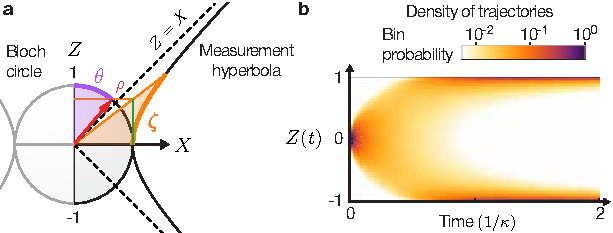
\includegraphics[scale=1.4]{mthry/CircleHyperbola}
\par\end{centering}
\caption[Random walk on the measurement hyperbola.]{\textbf{Random walk on the measurement hyperbola.\label{fig:Random-walk-on-hyperb}
a,} Circular and hyperbolic geometric representations of the pure
qubit state, $\rho$, parametrized by the circular and hyperbolic
angles $\theta$ and $\zeta$, respectively, obeying $\cos\left(\theta\right)=\tanh\zeta$.
The circle depicts a slice though the XZ plane of the Bloch sphere,
which is well-suited to represent unitary dynamics. The random walk
of $\zeta$ due to the measurement takes place on the unit hyperbola,
with asymptotes defined by the lines $Z=\pm X$. \textbf{b,} Histogram
of quantum trajectory densities obtained from simulations of the flying-spin
model. All trajectories (not shown here) begin with the initial state
defined by the Bloch coordinates $X\left(0\right)=1$ and $Z\left(0\right)=0$.
The time axis is scaled in units of the measurement rate, $\kappa$.
}
\end{figure}

The circular and hyperbolic coordinate transformations together with
Eqs.~(\ref{eq:SpinBathHRabi}) and~(\ref{eq:HyperbolicRotationMsr})
can be employed to construct a finite-difference numerical scheme
to calculate the quantum trajectory of the qubit subject to homodyne
monitoring. Notably, since the difference equations were derived \emph{without}
approximations, especially with regard to the size of $\Delta t$,
they guarantee a physical system state for all parameters and at all
time, features which offer some practical advantages for numerical
simulations. In the following subsection, Sec.~\ref{subsec:Continuous-limit:-Wiener},
we construct the continuum limit of the model and formally derive
the differential equations for the quantum trajectory of the qubit.


\subsection{Continuum limit: Wiener noise and stochastic calculus\label{subsec:Continuous-limit:-Wiener}}

In this section, we take the appropriate limit in which the measurement
becomes continuous. In this limit, the interaction time, $\Delta t$,
becomes infinitely small while the measurement strength, $\lambda$,
becomes infinitely large. Since each short sequence of individual
measurements carries an infinitesimal amount of information in this
limit, we coarse-grain the measurement record in the following way.
The evolution up to time $t$ is divided in $m$ intervals of total
duration $\dt$, while each of these intervals is further subdivided
in $l$ yet smaller intervals, each of duration $\Delta t$; i.e.,
$t=n\Delta t=ml\Delta t$ and $\dt=l\Delta t$. The interaction amplitude,
$\lambda$, is chosen to be $\lambda=\sqrt{\kappa/\Delta t}$, where
$\kappa$ denotes the interaction rate. Subject to appropriate scaling,
by a factor $\sqrt{\Delta t}$, the sum of all measurement results
up to time $t$ is the measurement signal $J_{t}=\sqrt{\Delta t}\sum_{m'=0}^{m}\sum_{l'=0}^{l}r_{m'l'}$.
During a time interval $\dt$, beginning at $t=ml\Delta t$ and ending
at $t'=\left(m+1\right)l\Delta t$, the signal changes by 
\begin{equation}
\mathrm{d}J_{t}=J_{\left(m+1\right)l\Delta t}-J_{ml\Delta t}=\sqrt{\Delta t}\sum_{k=ml}^{\left(m+1\right)l}r_{k}\:.\label{eq:dJ-stoch-diff-eq}
\end{equation}
Equation~(\ref{eq:dJ-stoch-diff-eq}) is known as a \emph{stochastic
difference equation, }because the difference increment in the variable
$J_{t}$ is a random variable. Assuming the state of the system does
not appreciably change over the time interval $\dt$, the measurement
results, $r_{k}$, are independent and identically distributed binary
random variables described by the probability function $\wp\left[r_{k}\right]=\frac{1}{2}\left(1-\epsilon r_{k}Z\left(t\right)\right),$
recall Eq.~(\ref{eq:PflyingSpinPM1}), where $\epsilon=\sqrt{\kappa\Delta t}$.
It follows that the mean and variance of the measurement increment
are 
\begin{align}
\E{\mathrm{d}J_{t}} & =l\sqrt{\Delta t}\E{r_{k}}=-\sqrt{\kappa}Z\left(t\right)\dt\,,\label{eq:EdJ-qubithomo}\\
\mathrm{Var}\left[\mathrm{d}J_{t}\right]= & l\Delta t\mathrm{Var}\left[r_{k}\right]\approx\dt\,,\label{eq:Var-dJ-qubithomo}
\end{align}
respectively, while, according to the central limit theorem, all higher-order
cumulants of the probability distribution for $\mathrm{d}J_{t}$ vanish
in the limit of large $l$. Working in this limit, and employing Eqs.~(\ref{eq:EdJ-qubithomo})
and~(\ref{eq:Var-dJ-qubithomo}), the stochastic difference equation,
Eq.~(\ref{eq:dJ-stoch-diff-eq}), can be taken to  the continuum
limit,\footnote{For completeness, we note that Eq.~(\ref{eq:QubitHomo:dJ}) is a
special case of Eq.~(\ref{eq:Jhom}). }

\begin{equation}
\boxed{\mathrm{d}J\left(t\right)=-\sqrt{\kappa}Z\left(t\right)\dt+\dW\left(t\right)\,},\label{eq:QubitHomo:dJ}
\end{equation}
where the infinitesimal term $\dW\left(t\right)$ represents Gaussian
white noise, and is known as the \emph{Wiener increment}. It obeys
the following canonical relations and probability density: 
\begin{align}
\E{\dW\left(t\right)} & =0\,, & \dW\left(t\right)\dt & =0\,,\label{eq:dW-relation-1}\\
\E{\dW\left(t\right)^{2}} & =\dt\,, & \wp\left(\dW\right) & =\frac{\exp\left(-\dW^{2}/(2\dt)\right)}{\sqrt{2\pi\dt}}\,.\label{eq:dW-relation-2}
\end{align}


\paragraph{Stochastic calculus. }

Equation~(\ref{eq:QubitHomo:dJ}) is known as a\emph{ stochastic
differential equation} (SDE) because the infinitesimal differential
is not completely determined, but is a random variable. Notably, in
obtaining this equation, we took the value of the function $Z\left(t\right)$
at the \emph{beginning} of the timestep $\dt$. In general, because
the stochastic noise is not smooth and not differentiable if we had
taken the value of the function at the\emph{ end} of the time-interval
$\dt$ we would have obtained a different form of the SDE. By taking
the value of the function at the beginning of the timestep, the SDE
we obtained is said to be in \emph{Itô form}; otherwise, it would
have been in \emph{Stratonovich form}. The two forms are not equivalent
in a straightforward manner, but for our purposes, it will suffice
to only consider the Itô form; see Chapter~3 of Ref.~\citet{Jacobs2010Book}
for an in-depth discussion. From Eqs.~(\ref{eq:dW-relation-1}) and
(\ref{eq:dW-relation-2}) it follows that the SDE solution only depends
on terms proportional to $\dt,$ $\dW,$ and $\dW^{2},$ while all
other terms of the form $\dt^{p}\dW^{q}$ are vanishing. Importantly,
in an unusual departure from the rules of differential calculus, in
the continuum limit, one can set $\dW^{2}=\dt$, a result known as
\emph{Itô}'s \emph{rule}. We note that $\dW\left(t\right)$ is an
idealized Gaussian noise process in that it has a perfect delta function
correlation in time, which implies its Markovianity, but also that
it has a white noise power spectral density, non-zero for \emph{all}
frequencies.


\paragraph{Itô SDE for the Bloch vector. }

In our example, the Bloch vector of the qubit can be parameterized\footnote{For simplicity, we have assumed $X\left(t\right)>0$ for all $t$.}
by its Z component, $\vec{S}\left(t\right)=\left(\sqrt{1-Z\left(t\right)^{2}},0,Z\left(t\right)\right)^{\intercal}$.
Thus, it suffices to derive an SDE for $Z\left(t\right)$, which is
obtained from the system state, $\ket{\psi_{J}\left(t\right)}$, conditioned
on the measurement signal $J\left(t\right)$ by taking the expectation
value of $\hat{\sigma}_{z}$, $Z\left(t\right)=\braOket{\psi_{J}\left(t\right)}{\hat{\sigma}_{z}}{\psi_{J}\left(t\right)}$.
The SDE is derived by first Taylor expanding $Z\left(t\right)=\cos\left(\theta\left(t\right)\right)$
to first order in $\dt$, $\mathrm{d}Z\left(t\right)\approx-\sqrt{1-Z\left(t\right)^{2}}\mathrm{d}\theta\left(t\right)-\frac{1}{2}Z\left(t\right)\mathrm{d}\theta\left(t\right)^{2}$,
where we have retained terms to second order in $\mathrm{d}\theta\left(t\right)$.
This is necessary because $\mathrm{d}\theta\left(t\right)$, recalling
Eq.~(\ref{eq:SPinBath:ThPM}), is proportional to $\dW$, and $\dW^{2}=\dt$.
By summing $l$ times over the difference equation and performing
the same coarse graining employed to arrive at Eq.~(\ref{eq:QubitHomo:dJ}),
we arrive at the Itô form of the SDE for the Z component of the Bloch
vector of a qubit subject to heterodyne monitoring of $\hat{\sigma}_{z}$,
\begin{equation}
\boxed{\mathrm{d}Z\left(t\right)=-\sqrt{\kappa}\left(1-Z\left(t\right)^{2}\right)\dW\left(t\right)\,.}\label{eq:QubitHomoToyConti}
\end{equation}
Equation~(\ref{eq:QubitHomoToyConti}) is a non-linear diffusion
equation with a state-dependent diffusion coefficient, $D\left(Z\right)=\kappa\left(1-Z^{2}\right)^{2}$,
which is maximized for $Z\left(t\right)=0$, but approaches zero for
$Z=\pm1$. Mathematically, it is for this reason, that in the limit
$t\rightarrow\infty$, the system tends to one of the pointer states
($Z=\pm1$) of the measurement, where diffusion vanishes, and states
cluster. 


\section{Quantum trajectory theory \label{sec:Quantum-trajectory-theory}}

The preceding sections introduced the general background required
to develop quantum trajectory theory. With the aid of specific examples,
important overriding themes were highlighted, which will carry us
forward in this section, and play a key role in understanding photon-counting,
homodyne, and heterodyne measurements. 


\subsection{Photodetection \label{subsec:Photodetection}}

Photodetection is the minimal time-continuous measurement scheme —
at each moment in time, the detector records one of only two possible
results: $r=0$ (``no-click'') or $r=1$ (``click''). As discussed
in Sec.~\ref{sec:Introductory-example:-qubit}, the measurement result
communicates some knowledge about the system state and the unavoidable
disturbance caused to it by the measurement itself.\footnote{From an operational point of view, the state of the system is strictly
speaking only \emph{our} knowledge about the probabilities for outcomes
of \emph{future} measurements of the system.} The information gain as well as the action of the disturbance are
encoded in the measurement operators, $\hat{M}_{r}$, recall Eq.~(\ref{eq:MrSpinBath}).
These operators, also known as Kraus operators, generalize unitary
evolution due to a system Hamiltonian, $\hat{H}$, so as to include
the effect of the measurement process. Microscopically, the measurement
operators, $\hat{M}_{r}$, can be understood to describe the unitary
interaction between the system and another, auxiliary one, which is
subsequently measured by a von Neumann measurement apparatus, see
discussion on Neumark's theorem in Sec.~\ref{sec:Introductory-example:-qubit}.
In this section, we will only concern ourselves with the system evolution
subject to measurement, and will make no further reference to the
auxiliary system, other than to specify the system operator $\hat{c}$
that couples the two. The minimal set of infinitesimal measurement
operators, which corresponding to the no-click ($r=0$) and click
($r=1$) evolution, are
\begin{align}
\hat{M}_{0}\left(\dt\right) & =\hat{1}-\left(\half\hat{c}^{\dagger}\hat{c}+i\hat{H}\right)\dt\,,\label{eq:photonM0}\\
\hat{M}_{1}\left(\dt\right) & =\sqrt{dt}\hat{c}\,,\label{eq:photonM1}
\end{align}
in units where $\hbar=1$. One can verify that $\hat{M}_{0}\left(\dt\right)$
and $\hat{M}_{1}\left(\dt\right)$ form a positive-operator-valued
measure (POVM) on the space of results. Hence, they form a resolution
of the identity, $\hat{M}_{0}^{\dagger}\left(\dt\right)\hat{M}_{0}\left(\dt\right)+\hat{M}_{1}^{\dagger}\left(\dt\right)\hat{M}_{1}\left(\dt\right)=\hat{1}+\mathcal{O}\left(\dt^{2}\right)$,
guaranteeing that the law of total probability is satisfied, i.e.,
a measurement yields an outcome with probability 1. The probability
for a specific outcome, $r=0$ or $r=1$, is is given by the generalized
measurement postulate, Eq.~(\ref{eq:GenMsrPosProb}), $\wp_{r}\left(\dt\right)=\left\langle \hat{M}_{r}^{\dagger}\left(\dt\right)\hat{M}_{r}\left(\dt\right)\right\rangle $,
\begin{align}
\wp_{0}\left(\dt\right) & =1-\dt\left\langle \hat{c}^{\dagger}\hat{c}\right\rangle +\mathcal{O}\left(\dt^{2}\right)\,,\label{eq:PhotonP0}\\
\wp_{1}\left(\dt\right) & =\dt\left\langle \hat{c}^{\dagger}\hat{c}\right\rangle \,.\label{eq:PhotonP1}
\end{align}
We define the time-continuous photodetection measurement record to
be the number of photodetections up to time $t$, denoted $N\left(t\right)$.
It follows that the infinitesimal measurement increment, denoted $\dN\left(t\right)$,
is a \emph{point-process}, also known as the \emph{Poisson process},
defined by 
\begin{align}
\dN\left(t\right)^{2} & =\dN\left(t\right)\,,\label{eq:Photon-dN-2}\\
\E{\dN\left(t\right)} & =\wp_{1}\left(\dt\right)\,,\label{eq:Photon-dN-E}
\end{align}
where $\E{\cdot}$ denotes the expectation value in the classical
sense, see Sec.~\ref{subsec:Classical-measurement-theory-basic-concept}.
In the continuum limit, the detector photocurrent, $I\left(t\right)=\dN\left(t\right)/\dt$,
consists of a series of Dirac $\delta$-functions at the times of
the clicks. 

\paragraph{Stochastic master equation (SME) for ideal photodetection. }

Ideal photodetection is the limit where the photodetector collects
the entirety of the system output field and adds no technical noise,
i.e., the quantum measurement efficiency is one, $\eta=1$. According
to the generalized projection postulate, Eq.~(\ref{eq:GenMsrPosProj}),
the state of the system after a measurement at time $t$ conditioned
on the measurement result $r=0$ or $r=1$ is 
\begin{equation}
\rho_{r}\left(t+\dt\right)=\frac{\hat{M}_{r}\left(\dt\right)\rho\left(t\right)\hat{M}_{r}^{\dagger}\left(\dt\right)}{\wp_{r}\left(\dt\right)}\,.\label{eq:click:rhoPLUS}
\end{equation}
In the continuum limit, where the instantaneous measurement outcome
is the photocurrent $I\left(t\right),$ the two possible states, $\rho_{0}\left(t+\dt\right)$
and $\rho_{1}\left(t+\dt\right)$, can be combined in a single stochastic
differential equation (SDE) for the posterior system state $\rho_{I}\left(t+\dt\right)$
conditioned on $I\left(t\right)$, resulting in the state differential,
in Itô form,
\begin{align}
\mathrm{d}\rho_{I}\left(t\right) & =\rho_{I}\left(t+\dt\right)-\rho_{I}\left(t\right)\\
 & =\dN\left(t\right)\left(\rho_{1}\left(t+\dt\right)-\hat{1}\right)+\left(1-\dN\left(t\right)\right)\left(\rho_{0}\left(t+\dt\right)-\hat{1}\right)\,,\label{eq:SME-prior}
\end{align}
which can be simplified by Taylor expanding the denominator of $\rho_{0}\left(t+\dt\right)$,
retaining terms to order $\dt$, and employing the stochastic calculus
rule\footnote{Technically, $\dN\left(t\right)\dt$ is not strictly zero. However,
because the mean of $\dN$ is infinitesimal, $\dN\left(t\right)$
is negligible when compared with $\dt$, and so are all higher-order
products containing both $\dN$ and $\dt$. }
\begin{equation}
\dN\left(t\right)\dt=0\,
\end{equation}
in order to obtain the \emph{stochastic master equation} (SME) for
photodetection, in the Schrödinger picture and in Itô form,
\begin{equation}
\boxed{\mathrm{d}\rho_{I}\left(t\right)=\left(\dN\left(t\right)\mathcal{G}\left[\hat{c}\right]+\dt\mathcal{H}\left[\hat{H}_{\mathrm{eff}}\right]\right)\rho_{I}\left(t\right)\,,}\label{eq:photon:SME}
\end{equation}
where the superoperators $\mathcal{G}\left[\hat{c}\right]\rho$ and
$\mathcal{H}\left[\hat{c}\right]\rho$ are defined by
\begin{align}
\mathcal{G}\left[\hat{c}\right]\rho\equiv & \frac{\hat{c}^{\dagger}\rho\hat{c}}{\Tr{\hat{c}^{\dagger}\rho\hat{c}}}-\rho\,,\label{eq:PhotoG}\\
\mathcal{H}\left[\hat{c}\right]\rho\equiv & \hat{c}\rho+\rho\hat{c}^{\dagger}-\Tr{\hat{c}\rho+\rho\hat{c}^{\dagger}}\rho\label{eq:PhotoH}\\
= & \left(\hat{c}-\left\langle \hat{c}\right\rangle \right)\rho+\rho\left(\hat{c}^{\dagger}-\left\langle \hat{c}^{\dagger}\right\rangle \right)\,,
\end{align}
The superoperator $\mathcal{G}$ results in point-like discontinuous
state evolution, while $\mathcal{H}$ results in smooth, continuous,
but non-unitary evolution generated by the effective non-Hermitian
Hamiltonian 
\begin{equation}
\hat{H}_{\text{eff}}\equiv\hat{H}-i\frac{1}{2}\hat{c}^{\dagger}\hat{c}\,.\label{eq:H_eff_noclick}
\end{equation}
Notably, the trace terms in Eqs.~(\ref{eq:PhotoG}) and (\ref{eq:PhotoH})
make the photodetection SME, Eq.~(\ref{eq:photon:SME}), \emph{nonlinear}
in the state density, $\rho_{I}$. The origin of the trace term in
$\mathcal{H}$, namely $\Tr{\hat{c}\rho+\rho\hat{c}^{\dagger}}$,
is the Taylor expansion of the denominator of Eq.~(\ref{eq:click:rhoPLUS}),
which gives the no-click probability, $\wp_{0}\left(\dt\right)$.
As discussed in Sec.~\ref{sec:Introductory-example:-qubit}, the
role of this term is to preserve the state density trace for all time,
$\Tr{\rho_{I}\left(t\right)}=1$. The solution of the SME is a stochastic
path taken by the conditional state over time, known as a \emph{quantum
trajectory}, a term\emph{ }coined in Ref.\emph{~\citet{Carmichael1993}. }

\paragraph{Stochastic Schrödinger equation (SSE) for photodetection. }

For a system in a pure state, $\rho_{I}\left(t\right)=\kb{\psi_{I}\left(t\right)}{\psi_{I}\left(t\right)}$,
the SME, Eq.~(\ref{eq:photon:SME}), preserves the purity of the
state for all times. It follows that the state evolution is described
by a type of Schrödinger equation, known as the \emph{stochastic Schrödinger
equation }(SSE), 
\begin{equation}
\boxed{\mathrm{d}\ket{\psi_{I}\left(t\right)}=\left[\dt\left(\frac{\left\langle \hat{c}^{\dagger}\hat{c}\right\rangle \left(t\right)}{2}-\frac{\hat{c}^{\dagger}\hat{c}}{2}-i\hat{H}\right)+\dN\left(t\right)\left(\frac{\hat{c}}{\sqrt{\left\langle \hat{c}^{\dagger}\hat{c}\right\rangle \left(t\right)}}-\hat{1}\right)\right]\ket{\psi_{I}\left(t\right)}\,,}\label{eq:SSE-click}
\end{equation}
which is nonlinear in the state $\ket{\psi_{I}\left(t\right)}$. The
non-linear terms contain the expectation value $\left\langle \hat{c}^{\dagger}\hat{c}\right\rangle \left(t\right)=\frac{1}{2}\braOket{\psi_{I}\left(t\right)}{\hat{c}^{\dagger}\hat{c}}{\psi_{I}\left(t\right)}$,
which gives the click probability $\wp_{1}$, see Eq.~(\ref{eq:PhotonP1}).
Because these non-linear terms render analytic treatment of the equations
particularly difficult in general, a linear description of the state
evolution is desired, and can be accomplished as described next. The
term $\frac{1}{2}\dt\left\langle \hat{c}^{\dagger}\hat{c}\right\rangle \left(t\right)\ket{\psi_{I}\left(t\right)}$,
which updates the observer's state-of-knowledge in a non-linear way,
mathematically, ensures the proper normalization of $\ket{\psi_{I}\left(t\right)}$
for all times; however, normalization need not be enforced for each
infinitesimal timestep $\dt$. Instead, it can ``manually'' be enforced
for the no-click periods, $I\left(t\right)=0$, by first first solving
for the un-normalized system state, denoted with a tilde, $\ket{\tilde{\psi}_{I=0}\left(t\right)}$,
then normalizing it, $\ket{\psi_{I=0}\left(t\right)}=\ket{\tilde{\psi}_{I=0}\left(t\right)}/\braket{\tilde{\psi}_{I=0}\left(t\right)}{\tilde{\psi}_{I=0}\left(t\right)}$,
where the effective Schrödinger equation for $\ket{\tilde{\psi}_{I=0}\left(t\right)}$
is
\begin{equation}
\boxed{i\frac{\mathrm{d}}{\dt}\ket{\tilde{\psi}_{I=0}\left(t\right)}=\hat{H}_{\mathrm{eff}}\ket{\tilde{\psi}_{I=0}\left(t\right)}\,,}\label{eq:SSE-click-1}
\end{equation}
where $\hat{H}_{\mathrm{eff}}$ is the non-Hermitian Hamiltonian,
Eq.~(\ref{eq:H_eff_noclick}). Since Eq.~(\ref{eq:SSE-click-1})
is linear, it is generally easier to solve for the time-dynamics.
Calculation of system averages still requires normalizing $\ket{\tilde{\psi}_{I=0}\left(t\right)}$
by its the state norm, $\braket{\tilde{\psi}_{I}\left(t\right)}{\tilde{\psi}_{I}\left(t\right)}$,
which gives the probability of no-clicks occurring for duration $t$.
We remark that Eq.~(\ref{eq:SSE-click-1}) corresponds to tracking
the sub-ensemble of quantum trajectories that contain no clicks, or
mathematically, to the repetitive application of the measurement operator
$\hat{M}_{0}$; hence, in general, in the limit $t\rightarrow\infty$,
it leads to the decay of the norm to zero. 

\paragraph{Unconditioned evolution: master equation for photodetection. }

By averaging over all possible evolutions due to all measurement outcomes
at each instant, one can obtain the \emph{unconditioned} evolution
of the quantum state, denoted $\rho\left(t+\dt\right)$, from Eq.~(\ref{eq:photon:SME}).
Simplifying the average, $\rho\left(t+\dt\right)=\sum_{r}\wp_{r}\rho_{r}\left(t+\dt\right)$,
\begin{align}
\rho\left(t+\dt\right) & =\hat{M}_{0}\left(\dt\right)\rho\hat{M}_{0}^{\dagger}\left(\dt\right)+\hat{M}_{1}\left(\dt\right)\rho\hat{M}_{1}^{\dagger}\left(\dt\right)\\
 & =\rho\left(t\right)-i\left[\hat{H},\rho\left(t\right)\right]\dt+\mathcal{D}\left[\hat{c}\right]\rho\left(t\right)\dt\,,\label{eq:MEforPhootdetection}
\end{align}
where the superoperator $\mathcal{D}$ is defined to be 
\begin{equation}
\mathcal{D}\left[\hat{c}\right]\rho\equiv\hat{c}\rho\hat{c}^{\dagger}-\frac{1}{2}\left\{ \hat{c},\rho\right\} _{+}\,.\label{eq:LindbladSuperop}
\end{equation}
Eq.~(\ref{eq:MEforPhootdetection}) for the unconditioned state evolution
is known as the \emph{master equation, }in Lindblad\emph{ }form \citep{lindblad1976}.\footnote{For a comprehensive summary of the properties of the master equation
and Lindbladians, see Refs.~\citet{AlbertVV2014-Lindblad,Albert2016-Lindblad}.} Unlike the SME, it is linear in the state density, $\rho$, and yields
deterministic state evolution, since there are no stochastic increments,
$\dN$ or $\dW$. Notably, the master equation is very general and
makes no reference to photodetection, other than specifying the system
operator $\hat{c}$ subject to detection, although it does not specify
how. As will be evident from the following section, the same master
equation is obtained for heterodyne detection of $\hat{c}$, see Sec.~\ref{subsec:Homodyne-and-heterodyne}.
The two SMEs corresponding to the same master equation are known as
\emph{unravellings}\footnote{The\emph{ }term 'unraveling' was coined in Ref. \citet{Carmichael1993}.}\emph{
}of it. We note that the unravellings of the master equation are not
unique.

\subparagraph{Imperfect detection.}

Imperfect conditions limit the observer's access to information regarding
the system and generally result in excess noise. The effect of imperfections
can be modeled by considering an ideal photodetector that is, however,
sensitive to only a fraction $\eta$ of the system output field. This
fraction, known as the \emph{quantum measurement efficiency}, is a
real number between zero and one, $0\leq\eta\leq1$. Because of the
loss of information due to imperfect detection, over time, the system
state will, in general, become mixed, with purity less than one, $0\leq\Tr{\rho^{2}}<1$.
To account for the imperfections, SME, Eq.~(\ref{eq:photon:SME}),
is be modified in the following way, see Sec.~4.8.1 of Ref.~\citet{wiseman2010book}:

\begin{equation}
\boxed{\mathrm{d}\rho_{I}\left(t\right)=\left(\dN\left(t\right)\mathcal{G}\left[\sqrt{\eta}\hat{c}\right]+\dt\mathcal{H}\left[-i\hat{H}-\eta\frac{1}{2}\hat{c}^{\dagger}\hat{c}\right]+\dt\left(1-\eta\right)\mathcal{D}\left[\hat{c}\right]\right)\rho_{I}\left(t\right)\,,}\label{eq:photon:SME-loss}
\end{equation}
where the jump probability for each timestep is obtained by also replacing
$\hat{c}$ with $\sqrt{\eta}\hat{c}$ in Eq.~(\ref{eq:Photon-dN-E}),
$\E{\dN\left(t\right)}=\eta\Tr{\hat{c}^{\dagger}\hat{c}\rho}\dt$.
Considering the two limits $\eta\rightarrow0$ and $\eta\rightarrow1$,
one can associate the Lindblad superoperator $\mathcal{D}$ with information
loss, and $\mathcal{H}$ and $\mathcal{G}$ with information gain
due to the measurement.


\subsection{Homodyne and heterodyne detection\label{subsec:Homodyne-and-heterodyne}}

The measurements described so far are not sensitive to the phase of
the system output field, but only its amplitude. In the following,
we describe \emph{dyne} measurements\emph{, homodyne} or \emph{heterodyne,
}which provide information about the phase and a qualitatively different
(diffusive) trajectory unraveling.

\paragraph{Physical implementation. }

Dyne detection is realized by mixing the system output signal with
a local-oscillator (LO) tone, see Fig.~\ref{fig:Schematic-representation-of}.
For a system carrier frequency, conventionally termed the radio frequency
(RF), $\omega_{\mathrm{RF}}$ and LO frequency $\omega_{\mathrm{LO}}$,
the lower sideband of the mixed-signal is at intermediate frequency
(IF), $\omega_{\mathrm{IF}}=\omega_{\mathrm{LO}}-\omega_{\mathrm{RF}}$.
In homodyne detection, the LO is tuned in resonance with the system
carrier, resulting in a direct-current (DC) IF signal, $\omega_{\mathrm{IF}}=0$,
proportional to a quadrate of the RF signal that depends on the LO
phase. The IF signal is typically sampled and digitally processed.
On the other hand, in heterodyne detection, the LO frequency is significantly
detuned from the RF, $\omega_{\mathrm{IF}}\gg0$, resulting in a an
oscillatory IF signal, which is demodulated to extract the information-bearing
\emph{in-quadrature} (I) and \emph{out-of-quadrature }(Q) components.
Note that the heterodyne measurement record consists of a series of
not one but \emph{ two} values, I and Q. Heterodyne detection is equivalent
to two concurrent homodyne detections with LO phases $90^{\circ}$
apart. 

\begin{figure}
\begin{centering}
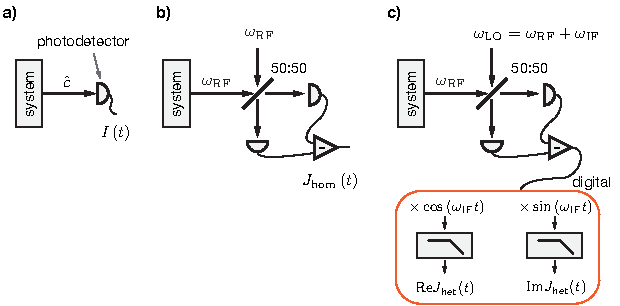
\includegraphics[scale=1.4]{mthry/Heterodyne2}
\par\end{centering}
\caption[Schematic representations of a photo, homodyne, and heterodyne detection
schemes.]{\label{fig:Schematic-representation-of}Schematic representations
of a (a) photo, (b) homodyne, and (c) heterodyne detection schemes.
\textbf{a, }The system output field, proportional to the system coupling
operator $\hat{c}$, is directly monitored with a photodetector, whose
photocurrent $I\left(t\right)$ is the measurement record. \textbf{b,}
Optical balanced homodyne detection: system output field, assumed
with carrier frequency $\omega_{\mathrm{RF}}$, is interfered on a
50:50 beam splitter with a strong local oscillator (LO) tone at the
carrier frequency, $\omega_{\mathrm{LO}}=\omega_{\mathrm{RF}}$. The
measurement record, $J_{\mathrm{hom}}\left(t\right)$, is obtained
from the  difference of the photodetector currents on each output
arm of the beamsplitter. \textbf{c,} Balanced heterodyne detection
scheme (with digital demodulation): LO frequency is detuned by an
intermediate frequency value, $\omega_{\mathrm{IF}},$ where $\omega_{\mathrm{IF}}\ll\omega_{\mathrm{RF}},\omega_{\mathrm{LO}}$.
The difference of the photodetector currents of each arm, which oscillates
at $\omega_{\mathrm{IF}}$, is digitally demodulated to obtain the
in-phase {[}out-of-phase{]} quadrature $\mathrm{Re}J_{\mathrm{het}}\left(t\right)$
{[}$\mathrm{Im}J_{\mathrm{het}}\left(t\right)${]} by digitally mixing
the signal with a reference one, $\cos\left(\omega_{\mathrm{IF}}t\right)$
{[}$\sin\left(\omega_{\mathrm{IF}}t\right)${]}, and low-pass filtering
the output to reject tones above $\omega_{\mathrm{IF}}$. Digital
panel schematic inspired by Ref.~\citep{Campagne2016-Fluorescence}.
}
\end{figure}


\paragraph{Homodyne measurement record. }

The homodyne measurement signal is mathematically described by a function,
$J_{\mathrm{hom}}\left(t\right)$, that is real and continuous everywhere
but differentiable nowhere, see Sec.~\ref{subsec:Continuous-limit:-Wiener}.
The measurement signal gradually reveals information about a system
operator of the form $\hat{c}+\hat{c}^{\dagger}$, where $\hat{c}$
is the operator coupled to the measurement apparatus, which for the
example of Sec.~\ref{subsec:Continuous-limit:-Wiener} is $\hat{c}=-\frac{\sqrt{\kappa}}{2}\hat{\sigma}_{z}$.
In Itô form, the measurement increment is
\begin{equation}
\mathrm{d}J_{\mathrm{hom}}\left(t\right)=\left\langle \hat{c}+\hat{c}^{\dagger}\right\rangle \left(t\right)\dt+\dW\left(t\right)\,,\label{eq:Jhom}
\end{equation}
where $\dW\left(t\right)$ is the stochastic Wiener increment satisfying
the canonical relations given in Eqs.~(\ref{eq:dW-relation-1})
and~(\ref{eq:dW-relation-2}).

\paragraph{Heterodyne measurement record. }

The heterodyne measurement signal consists of two functions: the in-phase,
$J_{I}\left(t\right)$, and out-of-phase, $J_{Q}\left(t\right)$,
quadrature functions, which can be combined in a single complex function,
$J_{\mathrm{het}}\left(t\right)\equiv\frac{1}{2}\left(J_{I}\left(t\right)+iJ_{Q}\left(t\right)\right)$,
continuous everywhere but differentiable nowhere.  In heterodyne
detection, $J_{\mathrm{het}}\left(t\right)$ gradually reveals information
about a system operator $\hat{c}$, which need not be Hermitian but
which can be decomposed into the sum of two Hermitian operators, corresponding
to two observables, know as the quadrature operators, 
\begin{equation}
\hat{I}\equiv\hat{c}+\hat{c}^{\dagger}\ \text{and}\ \hat{Q}\equiv-i\left(\hat{c}-\hat{c}^{\dagger}\right)\,,
\end{equation}
so that $\hat{c}=\frac{1}{2}\left(\hat{I}+i\hat{Q}\right)$. The Itô
form of the measurement increment is 
\begin{equation}
\mathrm{d}J_{\mathrm{het}}\left(t\right)=\left\langle \hat{c}\right\rangle \left(t\right)\dt+\dZ\left(t\right)\,,\label{eq:Jhet-perfect}
\end{equation}
where $\dZ\equiv\frac{1}{\sqrt{2}}\left(\dW_{I}\left(t\right)+i\dW_{Q}\left(t\right)\right)$
is the complex Wiener increment, the sum of two independent Wiener
increments, $\dW_{I}\left(t\right)$ and $\dW_{Q}\left(t\right)$,
that satisfy $\E{\dW_{I}\left(t\right)\dW_{Q}\left(t\right)}=0$,
so that $\dZ\left(t\right)^{*}\dZ\left(t\right)=\dt$ and $\dZ\left(t\right)^{2}=0$.
We note that $\dZ$ is obtained by making the substitution $e^{i\omega_{{\rm RF}}t}\dW\rightarrow\dZ$
in the heterodyne derivation.

For concreteness, consider the example of a qubit coupled to the environment
where an observer performs heterodyne detection of the qubit fluoresce
\citep{Campagne-Ibarcq2014,Campagne2016-Fluorescence,Naghiloo2016}.
The system-environment coupling is given by the non-Hermitian operator
$\hat{c}=\hat{\sigma}_{-}\equiv\kb{+z}{-z}$, which is decomposed
into the two Hermitian quadrature operators $\hat{I}=\hat{\sigma}_{x}$
and $\hat{Q}=-\hat{\sigma}_{y}$. Note the minus sign in $\hat{Q}$.
The heterodyne detection of $\hat{\sigma}_{-}$ can be understood
as a homodyne detection of the observable $\hat{I}$ and a concurrent
homodyne detection of the observable $\hat{Q}$, each with efficiency
$\eta=1/2$, see below. Consider the example where the qubit is replaced
by a cavity, the coupling operator is $\hat{c}=\hat{a}$, where $\hat{a}$
is the annihilation operator, and the whose cavity output field is
subject to heterodyne monitoring, which reveals information about
$\hat{I}=\hat{a}+\hat{a}^{\dagger}$ and $\hat{Q}=-i\left(\hat{a}-\hat{a}^{\dagger}\right)$.
For a coherent state in the cavity, $\ket{\alpha\left(t\right)}$,
the measurement record gradually reveals its complex amplitude, $\E{\mathrm{d}J_{\mathrm{het}}\left(t\right)/\dt}=\braOket{\alpha\left(t\right)}{\frac{1}{2}\left(\hat{I}+\hat{i}\hat{Q}\right)}{\alpha\left(t\right)}=\alpha\left(t\right)$. 

\paragraph{Measurement operators and the SME for perfect dyne detection.}

At an instant in time, the noisy heterodyne record, $J_{\mathrm{het}}\left(t\right)$,
relates the measurement outcome to the quantum trajectory evolution
according to the action of the measurement operator (see discussion
on Pg.~\pageref{eq:MrSpinBath})
\begin{equation}
\hat{M}_{J}=\hat{1}-i\hat{H}\dt-\frac{1}{2}\hat{c}^{\dagger}\hat{c}\dt+J_{\mathrm{het}}^{*}\left(t\right)\hat{c}\dt\,.\label{eq:hetero:msrmap}
\end{equation}
The measurement operator for homodyne detection, also denoted $\hat{M}_{J}$,
is obtained by making the substitution $J_{\mathrm{het}}^{*}\left(t\right)\rightarrow J_{\mathrm{hom}}\left(t\right)$
in Eq.~(\ref{eq:hetero:msrmap}). Notably, the non-orthogonal set
of measurement operators for dyne detection, $\left\{ \hat{M}_{J}:J\right\} $,
is continuous, in contrast with that of photodetection, which consists
of two elements, $\left\{ \hat{M}_{0},\hat{M}_{1}\right\} ,$ since
there are only two possible measurement outcomes, click or no click.
The system state conditioned on the record at time $t$, denoted $\rho_{J}$,
is obtained by employing the generalized measurement postulate, Eq.~(\ref{eq:GenMsrPosProj}),

\begin{equation}
\rho_{J}\left(t+\dt\right)=\frac{\hat{M}_{J}\rho_{J}\left(t\right)\hat{M}_{J}^{\dagger}}{\Tr{\hat{M}_{J}\rho_{J}\left(t\right)\hat{M}_{J}^{\dagger}}}\,.\label{eq:click:rhoPLUS-1}
\end{equation}
Equation~(\ref{eq:click:rhoPLUS-1}) is simplified by Taylor expanding
the denominator to order $\dt$ and writing the infinitesimal state
change, in Itô form, $\mathrm{d}\rho_{J}\left(t\right)=\rho_{J}\left(t+\dt\right)-\rho_{J}\left(t\right)$,
thus obtaining the SME for perfect heterodyne detection, in the Schrödinger
picture,
\begin{equation}
\mathrm{d}\rho_{J}\left(t\right)=\left[-i\dt[\hat{H},\cdot]+\dt\mathcal{D}[\hat{c}]+\dZ^{*}\left(t\right)\mathcal{H}[\hat{c}]\right]\rho_{J}\left(t\right)\,,\label{eq:SME-Heterodyne}
\end{equation}
where the superoperators $\mathcal{D}$ and $\mathcal{H}$ are defined
in Eqs.~(\ref{eq:LindbladSuperop}) and~(\ref{eq:PhotoH}), respectively.
Equation~(\ref{eq:SME-Heterodyne}) has to be solved jointly with
Eq.~(\ref{eq:Jhet-perfect}). The homodyne SME is obtained by making
the substitution $\dZ^{*}\left(t\right)\rightarrow\dW\left(t\right)$
in Eq.~(\ref{eq:SME-Heterodyne}).  

\paragraph{SME for imperfect measurements.}

Measurement imperfections (see discussion on Pg.~\ref{eq:photon:SME-loss})
are primarily due to: i) losses associated with the propagation of
the system output field to the measurement apparatus, characterized
by a quantum efficiency $\eta_{\mathrm{prop}}$, and ii) finite detector
efficiency, $\eta_{\mathrm{det}}$. The measurement chain efficiency
is given by the product of those of it sub-components, $\eta=\eta_{\mathrm{prop}}\eta_{\mathrm{det}}$,
and is used to modify Eq.~(\ref{eq:Jhet-perfect}) to account for
imperfections by making the substitution $\hat{c}\rightarrow\sqrt{\eta}\hat{c}$,
\begin{equation}
\boxed{\mathrm{d}J_{\mathrm{het}}\left(t\right)=\sqrt{\eta}\left\langle \hat{c}\right\rangle \left(t\right)\dt+\dZ\left(t\right)\,.}\label{eq:dJimperf:het}
\end{equation}
Similarly, the homodyne measurement increment is $\mathrm{d}J_{\mathrm{hom}}\left(t\right)=\sqrt{\eta}\left\langle \hat{c}+\hat{c}^{\dagger}\right\rangle \left(t\right)\dt+\dW\left(t\right)$.
In Eq.~(\ref{eq:dJimperf:het}), the effect of an efficiency less
than one, $\eta<1$, is to reduce the measurement signal amplitude,
$\left\langle \hat{c}\right\rangle $, relative to the noise, $\dZ$,
resulting in a degraded signal-to-noise (SNR) ratio. In the extreme
limit $\eta\rightarrow0$, the measurement is entirely noise, and
the SNR is zero. Only in the limit $\eta\rightarrow1$, as discussed
in Sec.~\ref{sec:Introductory-example:-qubit}, can the noise be
interpreted as entirely due to quantum vacuum fluctuations.  The
trajectory evolution associated with the noisy signal, $J_{\mathrm{het}}\left(t\right)$,
is obtained by making the substitution $\hat{c}\rightarrow\sqrt{\eta}\hat{c}$
in the innovator, $\mathcal{H}$, term of the heterodyne SME, Eq.~(\ref{eq:SME-Heterodyne}),
which is responsible for the information gain due to the measurement,
thus obtaining the SME for finite-efficiency heterodyne detection,
\begin{equation}
\boxed{\mathrm{d}\rho_{J}\left(t\right)=\left[-i\dt[\hat{H},\cdot]+\dt\mathcal{D}[\hat{c}]+\dZ^{*}\left(t\right)\mathcal{H}[\sqrt{\eta}\hat{c}]\right]\rho_{J}\left(t\right)\,,}\label{eq:SME-heterodyne-imperfect}
\end{equation}
which upon the the substitution $\dZ^{*}\left(t\right)\rightarrow\dW\left(t\right)$
becomes the SME for finite-efficiency homodyne detection. Equations~(\ref{eq:SME-heterodyne-imperfect})
and~(\ref{eq:dJimperf:het}) have to be solved simultaneously.

\subparagraph{Qualitative comparison of dyne- vs. photo- detection trajectories. }

In Sec.~\ref{subsec:Photodetection}, we considered the stochastic
evolution of the conditional quantum state of a system subject to
photodetection, a measurement scheme that results in one of two possible
outcomes, $r=0$ and $r=1$, at each moment in time. The state evolution
was marked by two qualitatively distinct possibilities: i) smooth,
continuous, deterministic-like evolution due to the non-Hermitian
Hamiltonian $\hat{H}_{\mathrm{eff}}$, associated with $r=0$, or
ii) discontinuous, point-like, jumpy evolution due to the action of
the superoperator term $\mathcal{G}$, associated with the occasional
outcome $r=1$. Both the measurement record and the state evolution
of dyne detection are, in a sense, antithetic to those of dyne detection,
which is characterized by a (Gaussian-distributed) infinite continuum
of possible measurement outcomes and neither smooth nor jumpy state
evolution. Rather, the evolution is \emph{diffusive} \citep{Gisin1992},
a consequence of the Gaussian-distributed measurement outcomes. While
in photodetection, a click could result in a substantial amount of
information about the system being acquired at an instant in time,
such an event is not possible with dyne monitoring, where the noisy
signal, $J\left(t\right)$, only \emph{gradually} reveals information
about the state of the system. It is only in this gradual sense that
dyne measurements collapse the system state to an eigenstate of the
measurement operator, see discussion of Sec.~\ref{subsec:Continuous-limit:-Wiener}. 


\section{Further reading \label{sec:Further-reading-traj-thry}}

For further reading, we suggest the following books, and, where applicable,
note sections closely related to some of the topics discussed in more
depth in this chapter:
\begin{itemize}
\item \citet{Carmichael1993} \& \citet{Carmichael2008-Book2} —  The formulation
of quantum trajectory theory is presented; key terms, such as 'unraveling',
are introduced. Section 17.2 of Ref.~\citet{Carmichael2008-Book2}
treats the example of a quantum bit subject to continuous photodetection,
comparing the state evolution in quantum measurement theory with that
of classical measurement theory. 
\item \citet{Gardiner2004} — Chapter~3 provides a useful derivation of
input-output theory by treating the one-dimensional transmission line.
Focus on the Heisenberg formulation of quantum measurements. 
\item \citet{wiseman2010book} — Classical measurement theory is introduced
in Chapter~2. 
\item \citet{Jacobs2010Book} — Introduction to \emph{classical} stochastic
differential equations (SDE).  
\item \citet{Girvin2014} — Chapter 3 discusses  quantum measurements
in the context of circuit quantum electrodynamics (cQED), which is
introduced in the remainder of the notes.
\item \citet{SteckQuantumNotes} — Lecture notes on quantum trajectories,
SDE numerical methods, and a number of related topics in quantum optics. 
\end{itemize}
We conclude this chapter with an amusing quote by H. Mabuchi:
\begin{center}
``\emph{The quantum measurement problem refers to a set of people}.''\\{[}the
set who have a problem with the theory of quantum measurements{]}
\citep{Fuchs2003-qminfo}.
\par\end{center}



\chapter{Theoretical description of quantum jumps\label{chap:theoretical-description-jumps} }

\addcontentsline{lof}{chapter}{Theoretical description of quantum jumps\lofpost}  
%\addcontentsline{lot}{chapter}{Theoretical description of quantum jumps\lofpost}

\singlespacing 
\setlength{\epigraphwidth}{.6\textwidth}
\epigraph{
Photons, the quanta of light, are countable and discrete, and one assumes they come and go in jumps. Einstein proposed it so --- though only as a pragmatic step  ... Yet the Schrödinger equation is deterministic and nothing within its jurisdiction jumps. What then to make of this unlikely marriage where the continuous is to somehow cavort with the discrete.}
{H.J. Carmichael\\New Zealand Science Review\\ Vol. 72 (2) 2015} 
\setlength{\epigraphwidth}{.4\textwidth} % default
\doublespacing\noindent\lettrine{T}{his} chapter presents the quantum trajectory
description of the Dehmelt electron-shelving scheme and the catch-and-reverse
circuit quantum electrodynamics (cQED) experiment. Section~\ref{sec:Fluorescence-monitored-by}
discusses quantum jumps in the three-level atom subject to fluorescence
photodetection. The minimal idealized model with coherent Rabi drives
is considered in Section \ref{sec:thry:3lvl-atom-simple-log}. To
better conceptualize important aspects of the measurement dynamics,
Sec.~\ref{subsec:Knowledge-driven-force-in} considers the simpler
case of a three-level atom subject only to measurement and no competing
coherent dynamics; i.e., the Dark Rabi drive is zero, $\Odg=0$. The
character of the unavoidable state-disturbance due to the back-action
of the measurement is examined in depth, and the notion of \emph{measurement-backaction
effective force} and its geometrical representation are introduced.
Section~\ref{subsec:Incoherent-Bright-drive} continues the description
of quantum jumps and considers the flight of the jump in the presence
of an incoherent Bright drive and the conditional interruption of
$\Odg$ ($\Delta t_{\mathrm{off}}$). Section~\ref{sec:Heterodyne-monitoring-of}
presents the trajectory description of the cQED experiment including
all known imperfections. Section~\ref{subsec:Simulation-of-linear}
discusses the Monte Carlo simulation of the linear Stochastic Schrödinger
equation (SSE), employed in the comparison between theoretical predictions
and experimental results, see Sec.~\ref{subsec:Comparison-between-theory}. 

\section{Fluorescence monitored by photon counts \label{sec:Fluorescence-monitored-by}}

\subsection{Dehmelt electron-shelving scheme and quantum jumps \label{sec:thry:3lvl-atom-simple-log}}

As discussed in Chapter~\ref{chap:Introduction-and-overview}, \textit{\emph{t}}he
experiments with trapped ions \citep{Nagourney1986,Sauter1986,Bergquist1986}
monitor intermittent fluorescence from the bright state $\B$ to track
jumps between $\G$ and $\D$ \citep{Cook1985}. In the simplest three-level
scheme \citep{Bergquist1986} and using coherent radiation to excite
both the BG and DG transitions, the master equation, Eq.~(\ref{eq:MEforPhootdetection}),
for the reduced density operator $\rho$ of the three-level system,
written in the interaction picture, is
\begin{equation}
\frac{\mathrm{d}\rho}{\dt}\left(t\right)=(i\hbar)^{-1}[\hat{H}_{{\rm drive}},\rho\left(t\right)]+\gamma_{{\rm B}}{\cal D}\left[\kb{\mathrm{G}}{\mathrm{B}}\right]\rho\left(t\right)+\gamma_{{\rm D}}{\cal D}\left[\kb{\mathrm{G}}{\mathrm{G}}\right]\rho\left(t\right),\label{eq:PhotonLindblad}
\end{equation}
where ${\cal D}[\hat{c}]\cdot=\hat{c}\cdot\hat{c}^{\dagger}-\frac{1}{2}\{\hat{c}^{\dagger}\hat{c},\cdot\}$
denotes the Lindblad superoperator, defined in Eq.~(\ref{eq:LindbladSuperop}),
$\gamma_{{\rm B}}$ and $\gamma_{{\rm D}}$ are radiative decay rates
of the B and D level, respectively, and the drive Hamiltonian is
\begin{equation}
\hat{H}_{{\rm drive}}=i\hbar\frac{\Omega_{{\rm BG}}}{2}\big(\kb{\mathrm{B}}{\mathrm{G}}-\kb{\mathrm{G}}{\mathrm{B}}\big)+i\hbar\frac{\Omega_{{\rm DG}}}{2}\big(\kb{\mathrm{D}}{\mathrm{G}}-\kb{\mathrm{G}}{\mathrm{D}}\big),\label{eq:drive_coherent_fluorescence}
\end{equation}
with $\Omega_{{\rm BG}}$ and $\Omega_{{\rm DG}}$ the Rabi drives.

\paragraph{Quantum trajectory description.}

The quantum trajectory description \citep{Carmichael1993,Dalibard1992-original-traj,Dum1992}
unravels $\rho$ into an ensemble of pure states, see Sec.~\ref{subsec:Photodetection},
whose ket vectors evolve along stochastic paths conditioned on the
clicks of \emph{imaginary} photon detectors that monitor fluorescence
from $\B$ and, much less frequently, from $\D$. Working in the limit
of the omniscient observer,  corresponding to unit quantum measurement
efficiency, $\eta=1$, for both the B and D click records, denoted
$\dN_{\mathrm{B}}\left(t\right)$ and $\dN_{\mathrm{D}}\left(t\right)$,
respectively, see Eqs.~(\ref{eq:Photon-dN-2}) and~(\ref{eq:Photon-dN-E}),
and corresponding to the quantum jump operators $\hat{c}_{\mathrm{B}}=\sqrt{\gamma_{{\rm B}}}\kb{\mathrm{G}}{\mathrm{B}}$
and $\hat{c}_{\mathrm{D}}=\sqrt{\gamma_{{\rm D}}}\kb{\mathrm{G}}{\mathrm{D}}$,
respectively, the non-linear stochastic Schrödinger equation (SSE)
in Itô form, Eq.~(\ref{eq:SSE-click}), is
\begin{align}
\mathrm{d}\ket{\psi_{I}\left(t\right)}= & \dt\left(-i\hat{H}+\frac{\gamma_{\mathrm{B}}}{2}\left(\left\langle \kb{\mathrm{B}}{\mathrm{B}}\right\rangle \left(t\right)-\kb{\mathrm{B}}{\mathrm{B}}\right)+\frac{\gamma_{\mathrm{D}}}{2}\left(\left\langle \kb{\mathrm{D}}{\mathrm{D}}\right\rangle \left(t\right)-\kb{\mathrm{D}}{\mathrm{D}}\right)\right)\ket{\psi_{I}\left(t\right)}\nonumber \\
 & +\dN_{\mathrm{B}}\left(t\right)\left(\frac{\kb{\mathrm{G}}{\mathrm{B}}}{\sqrt{\left\langle \kb{\mathrm{B}}{\mathrm{B}}\right\rangle \left(t\right)}}-\hat{1}\right)+\dN_{\mathrm{D}}\left(t\right)\left(\frac{\kb{\mathrm{G}}{\mathrm{D}}}{\sqrt{\left\langle \kb{\mathrm{D}}{\mathrm{D}}\right\rangle \left(t\right)}}-\hat{1}\right)\,.\label{eq:PhotonPsiI}
\end{align}
The terms proportional to $\dN_{\mathrm{B}}\left(t\right)$ and $\dN_{\mathrm{D}}\left(t\right)$
reset the ket vector to $\G$ with instantaneous probability $\gamma_{\mathrm{B}}\left\langle \kb{\mathrm{B}}{\mathrm{B}}\right\rangle \left(t\right)\dt$
and $\gamma_{\mathrm{D}}\left\langle \kb{\mathrm{D}}{\mathrm{D}}\right\rangle \left(t\right)\dt$,
respectively, and correspond to the state-disturbance due to the detection
of a click on the B and D detectors, respectively. Otherwise, when
no click is observed on either detector, the state follows a deterministic
evolution as a coherent superposition, governed by the terms proportional
to $\dt$. 

\paragraph{Linear SSE and no-click evolution. }

To describe the conditional no-click evolution, as discussed on Pg.~\pageref{eq:SSE-click-1},
it is analytically favorable to work with the linear form of the SSE,
obtained by suppressing the expectation value terms in Eq.~(\ref{eq:PhotonPsiI}),
and defining the \emph{un-normalized} quantum state, 
\begin{equation}
\ket{\tilde{\psi}\left(\Delta t_{{\rm catch}}\right)}=\cg\left(\Delta t_{{\rm catch}}\right)\G+\cb\left(\Delta t_{{\rm catch}}\right)\B+\cd\left(\Delta t_{{\rm catch}}\right)\D\,,\label{eq:GBD-ket}
\end{equation}
where $\Delta t_{{\rm catch}}$ denotes the no-click duration. Immediately
after a click, marked by $\deltatcatch=0$, the state $\ket{\tilde{\psi}\left(\Delta t_{{\rm catch}}\right)}$
is reset with the coefficients $\cg\left(\Delta t_{{\rm catch}}\right)=1$
and $\cb\left(\Delta t_{{\rm catch}}\right)=\cd\left(\Delta t_{{\rm catch}}\right)=0.$
Conditioned on no clicks, the evolution of the un-normalized state
is governed by the effective non-Hermitian Hamiltonian, see Eq.~(\ref{eq:H_eff_noclick}),
\begin{equation}
\hat{H}_{\mathrm{eff}}=\hat{H}_{{\rm drive}}-i\hbar\frac{\gamma_{{\rm B}}}{2}\kb{\mathrm{B}}{\mathrm{B}}-i\hbar\frac{\gamma_{{\rm D}}}{2}\kb{\mathrm{D}}{\mathrm{D}}\,,\label{eq:ClickHeff}
\end{equation}
and the Schrödinger-type equation 
\begin{equation}
i\hbar\frac{\mathrm{d}\ket{\tilde{\psi}\left(\Delta t_{{\rm catch}}\right)}}{\mathrm{d}\Delta t_{{\rm catch}}}=\hat{H}_{\mathrm{eff}}\ket{\tilde{\psi}\left(\Delta t_{{\rm catch}}\right)}\,.\label{eq:NonHermitianShcr}
\end{equation}
Due to the purely imaginary-valued terms in $\hat{H}_{\mathrm{eff}}$,
the norm of the state $\ket{\tilde{\psi}\left(\Delta t_{{\rm catch}}\right)}$
decays as a function of $\Delta t_{{\rm catch}}$ and gives the probability
that the no-click evolution has continued without click interruptions
for duration $\Delta t_{{\rm catch}}$. In  the limit $\deltatcatch\rightarrow0$,
the norm of the ket approaches zero. The evolution of the state can
be described by a matrix equation for the state coefficients, using
Eqs.~(\ref{eq:GBD-ket}), (\ref{eq:ClickHeff}), and~(\ref{eq:NonHermitianShcr}),
\begin{equation}
\frac{\mathrm{d}}{\mathrm{d}\Delta t_{{\rm catch}}}\begin{pmatrix}\cg\\
\cb\\
\cd
\end{pmatrix}=\frac{1}{2}\left(\begin{matrix}0 & -\Omega_{{\rm BG}} & -\Omega_{{\rm DG}}\\
\Omega_{{\rm BG}} & -\gamma_{{\rm B}} & 0\\
\Omega_{{\rm DG}} & 0 & -\gamma_{{\rm D}}
\end{matrix}\right)\begin{pmatrix}\cg\\
\cb\\
\cd
\end{pmatrix}.\label{eqn:3x3_system}
\end{equation}
In general this $3\times3$ system does not have a closed solution
in simple form, although there is a particularly simple solution under
conditions that produce intermittent fluorescence, i.e., rare jumps
from $\G$ to $\D$ {[}``shelving'' in the dark state \citep{Nagourney1986}{]}
interspersed as intervals of fluorescence ``off'' in a background
of fluorescence ``on''. The conditions follow naturally if $\D$
is a metastable state \citep{Nagourney1986,Sauter1986,Bergquist1986}
whose lifetime $\gamma_{{\rm D}}^{-1}$ is extremely long on the scale
of the mean time, 
\begin{equation}
\tau_{\mathrm{BG}}=\frac{\Omega_{{\rm BG}}^{2}}{\gamma_{\mathrm{B}}}\,,\label{eq:GammaBG}
\end{equation}
between photon detector clicks for a weak $\Omega_{{\rm BG}}$ Rabi
drive. Subject to $(\Omega_{{\rm DG}},\gamma_{{\rm D}})\ll\Omega_{{\rm BG}}^{2}/\gamma_{{\rm B}}\ll\gamma_{{\rm B}}$,
one way to solve Eq.~(\ref{eqn:3x3_system}) is to first adiabatically
eliminate the fast time dynamics of the B level, by setting the time
derivative of the B coefficient to zero, 
\begin{eqnarray}
\frac{\mathrm{d}\cb}{\mathrm{d}\Delta t_{{\rm catch}}} & = & 0\,,\label{eq:Cbadiabatic}
\end{eqnarray}
Solving Eq.~(\ref{eq:Cbadiabatic}), $\cb=\frac{\Omega_{\mathrm{BG}}}{\gamma_{\mathrm{B}}}\cg$,
allows one to eliminate the B level from the description of the dynamics
and to extract the effective GD dynamics, to obtain the un-normalized
state conditioned on the detection of no clicks,
\begin{align}
\ket{\tilde{\psi}\left(\deltatcatch\right)}= & \exp\left(-\frac{\Omega_{{\rm BG}}^{2}}{2\gamma_{\mathrm{B}}}\deltatcatch\right)\left(\G+\frac{\Omega_{\mathrm{BG}}}{\gamma_{\mathrm{B}}}\B\right)\nonumber \\
 & +\left[\exp\left(-\frac{\gamma_{\mathrm{D}}}{2}\deltatcatch\right)-\exp\left(-\frac{\Omega_{{\rm BG}}^{2}}{2\gamma_{\mathrm{B}}}\deltatcatch\right)\right]\frac{\gamma_{\mathrm{B}}\Omega_{\mathrm{D}}}{\Omega_{{\rm BG}}^{2}}\D\,.\label{eq:psiPhotonNoClick}
\end{align}
Note that $\ket{\tilde{\psi}\left(\deltatcatch\right)}$ has purely
real coefficients, since $\hat{H}_{\mathrm{eff}}$ has purely imaginary
ones. The Bloch vector components of the normalized GD manifold evolution
conditioned on no-clicks are obtained by normalizing the state, Eq.~(\ref{eq:psiPhotonNoClick}),
\begin{eqnarray}
{\rm Z}_{{\rm GD}}(\Delta t_{{\rm catch}}) & = & \frac{W_{{\rm DG}}(\Delta t_{{\rm catch}})-W_{{\rm DG}}^{-1}(\Delta t_{{\rm catch}})}{W_{{\rm DG}}(\Delta t_{{\rm catch}})+W_{{\rm DG}}^{-1}(\Delta t_{{\rm catch}})},\label{eqn:Z}\\
{\rm X}_{{\rm GD}}(\Delta t_{{\rm catch}}) & = & \frac{2}{W_{{\rm DG}}(\Delta t_{{\rm catch}})+W_{{\rm DG}}^{-1}(\Delta t_{{\rm catch}})},\label{eqn:X}\\
{\rm Y}_{{\rm GD}}(\Delta t_{{\rm catch}}) & = & 0,\label{eqn:Y}
\end{eqnarray}
where we have defined the ratio \citep{Porrati1987}
\begin{equation}
W_{{\rm DG}}(\Delta t_{{\rm catch}})\equiv\frac{\cd(\Delta t_{{\rm catch}})}{\cg(\Delta t_{{\rm catch}})}.\label{eqn:W_DG_definition}
\end{equation}
Notably, as an alternative to the adiabatic method employed to solve
Eq.~(\ref{eqn:3x3_system}), one can instead directly write down
the equation of motion for $W_{{\rm DG}}$ within the same approximations,
\begin{equation}
\frac{\mathrm{d}W_{{\rm DG}}}{\mathrm{d}\Delta t_{{\rm catch}}}=\frac{\Omega_{{\rm BG}}^{2}}{2\gamma_{{\rm B}}}W_{{\rm DG}}+\frac{\Omega_{{\rm DG}}}{2},\label{eqn:W_DG_equation_coherent}
\end{equation}
which, with the initial condition $W_{{\rm DG}}(0)=0$, has the solution
\begin{equation}
W_{{\rm DG}}(\Delta t_{{\rm catch}})=\frac{\Omega_{{\rm DG}}}{\Omega_{{\rm BG}}^{2}/\gamma_{{\rm B}}}\left[\exp\left(\frac{\Omega_{{\rm BG}}^{2}}{2\gamma_{{\rm B}}}\Delta t_{{\rm catch}}\right)-1\right],\label{eq:WDG-coh}
\end{equation}
and also yields the Bloch components, Eqs.~(\ref{eqn:Z}), (\ref{eqn:X}),
and~(\ref{eqn:Y}). The timescale of the transition, the mid-flight
time of the quantum jump, $\Delta t_{{\rm mid}}$, is found by setting
the G and D coefficients equal to each other, $\cg\left(\Delta t_{{\rm mid}}\right)=\cd\left(\Delta t_{{\rm mid}}\right),$
\begin{equation}
\boxed{\Delta t_{{\rm mid}}=\left(\frac{\Omega_{{\rm BG}}^{2}}{2\gamma_{{\rm B}}}\right)^{-1}\ln\left(\frac{\Omega_{{\rm BG}}^{2}/\gamma_{{\rm B}}}{\Omega_{{\rm DG}}}+1\right).}\label{eq:t_mid_coherent}
\end{equation}
For strong monitoring, $\Omega_{{\rm BG}}^{2}\gamma_{{\rm B}}^{-1}\gg\Omega_{{\rm DG}}$,
the +1 in Eq.~(\ref{eq:t_mid_coherent}) can be dropped. Working
in this limit, Eqs.~(\ref{eqn:Z})–(\ref{eqn:Y}) provide simple
formulas for the continuous, deterministic, and coherent evolution
of the completed quantum jump:
\begin{eqnarray}
{\rm Z}_{{\rm GD}}(\Delta t_{{\rm catch}}) & = & {\rm tanh}\left[\frac{\Omega_{{\rm BG}}^{2}}{2\gamma_{B}}(\Delta t_{{\rm catch}}-\Delta t_{{\rm mid}})\right],\label{eqn:Z_approx}\\
{\rm X}_{{\rm GD}}(\Delta t_{{\rm catch}}) & = & {\rm sech}\left[\frac{\Omega_{{\rm BG}}^{2}}{2\gamma_{B}}(\Delta t_{{\rm catch}}-\Delta t_{{\rm mid}})\right],\label{eqn:X_approx}\\
{\rm Y}_{{\rm GD}}(\Delta t_{{\rm catch}}) & = & 0.\label{eqn:Y_approx}
\end{eqnarray}
These formulas, derived in the strong-monitoring limit, execute a
perfect jump, ${\rm Z}_{{\rm GD}}(\infty)=1$, ${\rm X}_{{\rm GD}}(\infty)={\rm Y}_{{\rm GD}}(\infty)=0$.
Departures from the ideal limit can be transparently analyzed by adopting
an incoherent Bright drive, see Sec.~\ref{subsec:Incoherent-Bright-drive}.
An elegant analysis of the no-click evolution for arbitrary amplitude
of the Dark Rabi drive can be found in Refs.~\citet{Ruskov2007}
and~\citet{Ruskov2009-unpublished}. For an interesting connection
to of the three-level intermittent dynamics to dynamical phase transitions,
see Refs.~\citet{Lesanovsky2013} and~\citet{Garrahan2018}.
\begin{figure}
\begin{centering}
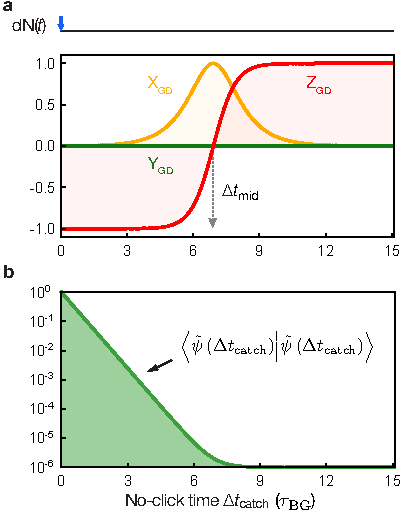
\includegraphics[scale=1.4]{qmjump/ideal_jump}
\par\end{centering}
\caption[Conditional no-click evolution of the jump from $\G$ to $\D$: ideal
photodetection theory.]{\textbf{\label{fig:Conditional-no-click-evolution}Conditional no-click
evolution of the jump from $\G$ to $\D$: ideal photodetection theory.
a, }A typical quantum trajectory for a jump from $\G$ to $\D$ represented
as the GD Bloch vector ($X_{\mathrm{GD}}$, $Y_{\mathrm{GD}}$, $Z_{\mathrm{GD}}$),
conditioned on \emph{no }clicks, $\dN\left(t\right)=0$, for duration
$\deltatcatch$. The Rabi drives are $\Omega_{\mathrm{DG}}=10^{-5}$
and $\Omega_{\mathrm{BG}}=0.1$ in units of the decay rate $\gamma_{\mathrm{B}}$.
Time axis is scaled in units of the mean time between detector clicks,
$\tau_{\mathrm{BG}}=(\Omega_{{\rm BG}}^{2}/\gamma_{\mathrm{B}})^{-1}$.
Time scale of the jump flight is the mid-flight time $\Delta t_{\mathrm{mid}}$,
defined by $Z_{\mathrm{GD}}=0$. \textbf{b,} Log plot of the norm
of the un-normalized no-click state, $\braket{\tilde{\psi}\left(\Delta t_{\mathrm{catch}}\right)}{\tilde{\psi}\left(\Delta t_{\mathrm{catch}}\right)}$,
as a function of $\deltatcatch$, in units of $\tau_{\mathrm{BG}}$.
Parameters of the plot correspond to those of panel a. }
\end{figure}


\paragraph{Remarks on the state evolution. }

The evolution of the GD manifold Bloch vector ($X_{\mathrm{GD}}\left(\deltatcatch\right),$
$Y_{\mathrm{GD}}\left(\deltatcatch\right),$ $Z_{\mathrm{GD}}\left(\deltatcatch\right)$)
conditioned on \emph{no }clicks, $\dN\left(\deltatcatch\right)=0$,
for duration $\deltatcatch$, is plotted in Fig.~\ref{fig:Conditional-no-click-evolution}a.
The partial tomogram visually shows that the predicted evolution of
the quantum jump from $\ket{\mathrm{G}}$ to $\ket{\mathrm{D}}$ is
continuous and coherent, $X_{\mathrm{GD}}^{2}+Y_{\mathrm{GD}}^{2}+Z_{\mathrm{GD}}^{2}=1$
for all no-click times, $\deltatcatch$. The measurement record, $\dN$,
and the predicted trajectory is identical for any two jumps from $\G$
to $\D$. The time axis has been scaled in units of the mean time,
$\tau_{\mathrm{BG}}=(\Omega_{{\rm BG}}^{2}/\gamma_{\mathrm{B}})^{-1}$,
between photon detector clicks. This time can also be understood as
the inverse of the information-gain rate of the measurement about
the G level. To expand on this, for definitiveness, consider the situation
where the atom is initialized in $\G$, but this information is not
shared with the observer operating the photon detector. By measurement,
how long does it take the observer to statistically deduce that the
atom is in $\G$ or not?  The measurement drive $\Omega_{\mathrm{BG}}$
is actuated and the observer  monitors the detector for clicks. If
the atom is in $\G,$ on average, the detector records a click after
time $\tau_{\mathrm{BG}}$, and informs the observer that the atom
is definitively in $\G$. Alternatively, if the atom was initialized
in $\D,$ no clicks would be recorded. As the detector does not record
a click for durations longer than $\tau_{{\rm BG}}$, the observer
becomes increasingly confident that the atom could not be in $\G$
since it becomes exponentially unlikely that a click has not yet been
observed, see Fig.~\ref{fig:Conditional-no-click-evolution}b, and
the alternative conclusion, that the atom is in $\D$, becomes increasingly
likely. Although this information-gain consideration is carried out
from the point of view of the observer, and with classical measurements
would bear no consequence for the objective state of the system, with
quantum measurements the gain of information about the system by virtue
of a measurement is necessarily accompanied by a result-correlated
state-disturbance (back-action). In Hilbert space, the disturbance
can be viewed as a \emph{measurement-backaction effective force},
as discussed in the following subsection, Sec.~\ref{subsec:Knowledge-driven-force-in}.

\paragraph{Probability of no-click record.}

Fig.~\ref{fig:Conditional-no-click-evolution}b shows a plot of the
conditional no-click state norm, $\braket{\psi\left(\deltatcatch\right)}{\psi\left(\deltatcatch\right)}$,
as a function of the no-click duration, $\deltatcatch$. The norm
initially decays exponentially with a time-constant $\tau_{{\rm BG}}$,
during which time, the atom remains essentially in $\G$, as indicated
by the $Z_{{\rm GD}}$ Bloch component in panel a, which is roughly
equal to $-1$. However, as the no-click duration approaches  mid-flight
time of the jump, $\deltatcatch\approx\Delta t_{{\rm mid}}$, the
decay of the norm slows down dramatically, since the atom transitions
from $\G$ to $\D$, in which state one can stop expecting the rapid
occurrence of clicks. The quantum jump from $\G$ to $\D$ can be
observed in the tomogram shown in panel (a). For no-click duration
$\deltatcatch\gg\Delta t_{{\rm mid}}$, the decay of the norm initially
appears flat, however, on longer time-scales (not shown) it is seen
that it also follows an exponential decay law with a much longer time
constant, $\tau_{{\rm DG}}\gg\tau_{{\rm BG}}$, corresponding to the
waiting-time for the jump back down, from $\D$ to $\G$.

\paragraph{\textit{\emph{Application of the photon counting model to the experiment.}}}

The photon-counting theory presented in this section provides the
background to the experiment along with a link to the original ion
experiments. It captures a core set of the ideas, even though the
monitoring of $|{\rm B\rangle}$ implemented in the experiment is
diffusive — the opposite limit of the point-process description presented
here, see Sec.~\ref{sec:Heterodyne-monitoring-of}. Nevertheless,
the photon-counting theory even provides a quantitative first approximation
of the experimental results. For definitiveness, consider the flight
of the quantum jump shown in Fig.~\ref{fig:catch}b. The measured
mid-flight time, $\Delta t_{\mathrm{mid}}=3.95~\mathrm{\mu s}$, is
predicted, in a first approximation, by Eq.~(\ref{eq:t_mid_coherent}).
Using the (independently measured) values of the experimental parameters,
summarized in Table~\ref{tab:system-params} (setting $\Omega_{\mathrm{BG}}$
equal to $\Omega_{\mathrm{B0}}=2\pi\times1.2$~MHz, the BG drive
when the atom is not in $\ket{\rm B}$) and extracting the effective
measurement rate of $|{\rm B\rangle}$, $\gamma_{\mathrm{B}}=2\pi\times9.0$~MHz
(which follows from Eq.~(\ref{eq:GammaBG}) where $\Gamma_{\mathrm{BG}}=2\pi\times1.01$~MHz,
the average click rate on the BG transition), Eq.~(\ref{eq:t_mid_coherent})
predicts $\Delta t_{{\rm mid}}\approx4.3~\mathrm{\mu s}$ — in fair
agreement with the observed value $\Delta t_{{\rm mid}}=3.95~\mathrm{\mu s}$.
The photodetection theory presented in in Sec.~\ref{subsec:Incoherent-Bright-drive}
further improves the agreement. These calculations serve to generally
illustrate the theory and ideas of the experiment; the quantitative
comparison between theory and experiment is only presented in Sec.~\ref{subsec:Comparison-between-theory}.

\subsection{Measurement-backaction effective force in the absence of the Dark
Rabi drive\label{subsec:Knowledge-driven-force-in}}

While in Sec.~\ref{sec:thry:3lvl-atom-simple-log} we considered
the coherent dynamics of the three-level atom in the presence of  both
unitary evolution, due to the Rabi drive $\Odg$, and the competing
non-unitary state collapse, due to the measurement, in this subsection,
we examine the simpler case where only measurement dynamics are at
play, i.e., $\Odg=0$. In this simpler situation, some important features
of the measurement, consisting of the Rabi drive $\Obg$ and the monitoring
of the B level at the rate $\gamma_{{\rm B}}$, are more easily discussed.
In particular, we pay attention to the notion of a\emph{ measurement-backaction
effective force}, the special force that unavoidably disturbs of the
quantum state due to the measurement. 

For definitiveness, consider the situation where  the three-level
atom is prepared in an initial superposition involving the G and D
levels, $\ket{\psi\left(0\right)}=\mathcal{N}\left(\G+\epsilon\D\right)$,
where $\epsilon\ll1$ and $\mathcal{N}$ is the ket normalization
factor; for simplicity, assume $\D$ is completely decoupled form
the environment, $\gamma_{{\rm D}}=0$. To measure the atom, only
the Rabi drive $\Obg$ is turned on. One of two qualitatively distinct
measurement records is observed: either clicks are recorded indefinitely
or no clicks are ever recorded, which can qualitatively be understood
in view of the following considerations. When the BG drive is first
turned on, some of the initial population from the G level is transferred
to the B level due to the steering force of $\Obg$. However, even
as a tiny amount of population is deposited in $\B$, the strong coupling
with the environment and the photodetector dampens the transfer and
quickly yields the detection of a click, with probability $\wp_{1}\left(\dt\right)=\left\langle \hat{c}_{{\rm B}}^{\dagger}\hat{c}_{{\rm B}}\right\rangle \left(t\right)\dt$,
where $\hat{c}_{\mathrm{B}}=\sqrt{\gamma_{{\rm B}}}\kb{\mathrm{G}}{\mathrm{B}}$
is the  jump operator. The click resets the atom to the ground state,
$\G$. Once the atom is completely in $\G$, the amplitude of $\D$
is zero, and since $\Odg=0$, the atom can never transition to $\D$
subsequently. The remainder of the history proceeds as described above,
the atom remains predominantly in $\G$ and continues to fluoresce
though the partial excitation and subsequent relaxation of $\B$,
by means of $\Obg$ and the detection, $\gamma_{{\rm B}}$, respectively.
In this way, the Dehmelt electron scheme implements a measurement
with result $\G$, occurring with an approximate probability $1-\epsilon^{2}$.
The alternative set of trajectories, where no clicks are observed
is quantitatively analyzed in the following, and occur with approximate
probability $\epsilon^{2}$.

\paragraph{No-click trajectory. }

The \emph{normalized} state of the three-level atom conditioned on
no-clicks, \footnote{Notationally, we employ capital letters for the coefficients of the
normalized sate, and lower-case letters for those of the un-normalized
state.} 
\begin{equation}
\ket{\psi_{I=0}\left(t\right)}=\cgn\left(t\right)\G+\cbn\left(t\right)\B+\cdn\left(t\right)\D\,,\label{eq:psiPhotonNL}
\end{equation}
evolves according to the non-linear Schrödinger equation, see Eq.~(\ref{eq:psiPhotonNoClick}),
\begin{equation}
\frac{\mathrm{d}}{\mathrm{d}t}\ket{\psi_{I=0}\left(t\right)}=\left(-i\hat{H}-\half\hat{c}_{{\rm B}}^{\dagger}\hat{c}_{{\rm B}}+\half\left\langle \hat{c}_{{\rm B}}^{\dagger}\hat{c}_{{\rm B}}\right\rangle \left(t\right)\right)\ket{\psi_{I=0}\left(t\right)}\:,\label{eq:NL-SSe-Cond-3}
\end{equation}
which in terms of the normalized state coefficients ($\cgn,\cbn$,
and $\cdn$) yields the set of coupled non-linear equations,
\begin{align}
\ddt\cbn\left(t\right)= & \frac{1}{2}\gamma_{{\rm B}}\cbn\left(t\right)^{3}+\frac{1}{2}\Omega_{{\rm BG}}\cgn\left(t\right)-\half\gamma_{{\rm B}}\cbn\left(t\right),\label{eq:Cbn}\\
\ddt\cgn\left(t\right)= & \frac{1}{2}\gamma_{{\rm B}}\cbn\left(t\right)^{2}\cgn\left(t\right)-\frac{1}{2}\Omega_{{\rm BG}}\cbn\left(t\right),\label{eq:Cgn}\\
\ddt\cdn\left(t\right)= & \frac{1}{2}\gamma_{{\rm B}}\cbn\left(t\right)^{2}\cdn\left(t\right),\label{eq:Cdn}
\end{align}
The measurement terms in Eqs.~(\ref{eq:Cbn})-(\ref{eq:Cdn}) associated
with information gain are the non-linear ones. As discussed in Sec.~\ref{sec:Quantum-trajectory-theory},
they originate from the normalization term in the conditional state
update and give rise to non-unitary state dynamics, resulting in a
drastic departure from the usual Schrödinger equation. To analyze
their effect and gain some physical intuition, we introduce a graphical
representation of the Hilbert space of the three-level atom.

\paragraph{$\mathbb{R}$-qutrit sphere representation. }

It follows from the real coefficients of Eqs.~(\ref{eq:Cbn})-(\ref{eq:Cdn})
and the initial conditions that $\cgn,\cbn,$ and $\cdn$ are constrained
to be real. Hence a pure state of the atom admits a geometrical representation
as a point on the unit sphere defined by the state norm condition
$\cbn^{2}+\cgn^{2}+\cdn^{2}=1$, see Fig.~\ref{fig:R-qutrit-sphere-representation.}.
We nickname this representation the '$\mathbb{R}$-qutrit sphere'.
Unlike the Bloch sphere representation where orthogonal state vectors
are represented by \emph{antiparallel} vectors, in the $\mathbb{R}$-qutrit
sphere representation, orthogonal state vectors are actually represented
by orthogonal vectors, extending from the origin to the surface of
the sphere. Notably, the sphere contains states of the two-level sub-manifolds
that are \emph{not} represented on the Bloch sphere, those with a
``global phase.''\footnote{The special unitary Lie group $SU(2)$ is not isomorphic to the special
orthogonal Lie group $SO(3)$, but is a double cover of it.} The addition of the third level allows, in general, the observation
of the global phase because it can be measured relative to the phase
of the third level. Consequently, a Rabi rotation between two levels
is no longer $2\pi$ periodic but $4\pi$ periodic.  Unitary evolution
is represented by rotations on the sphere; for instance, the evolution
due to the Bright Rabi drive, $\Obg$, is a rotation about the D axis,
and the corresponding infinitesimal-state-change vector field, $\mathrm{d}\ket{\psi}\left(\Obg\right)=\frac{1}{2}\left(\cgn\B-\cbn\G\right)\Obg\dt$,
is plotted on the surface of the sphere in Fig.~\ref{fig:R-qutrit-sphere-representation.}.
Note that the length of the vectors is largest at the GB equator and
approaches zero toward the D poles. The vector field representation
is useful in the analysis of the non-linear measurement-backaction
effective force  due to the renormalization terms and we hope can
provide a more intuitive understanding of the interplay between the
coherent Rabi and the stochastic measurement dynamics.  Before elaborating
on the geometrical representation of the measurement dynamics, it
is useful to first algebraically solve Eqs.~(\ref{eq:Cbn})-(\ref{eq:Cdn}).

\begin{figure}
\begin{centering}
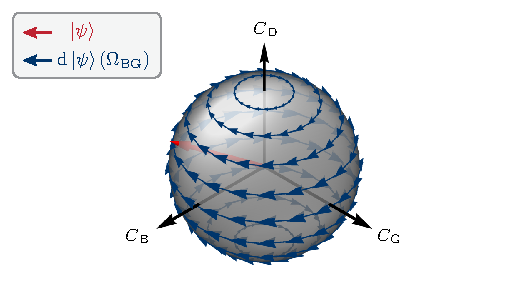
\includegraphics[scale=1.5]{qmjump/knowledge_sphere}
\par\end{centering}
\caption[Geometrical representation of a qutrit state with real coefficients:\textbf{
$\mathbb{\mathbb{R}}$}-qutrit sphere]{\label{fig:R-qutrit-sphere-representation.}\textbf{Geometrical representation
of a qutrit state with real coefficients:} $\mathbb{\mathbb{R}}$\textbf{-qutrit
sphere. }Geometric representation of the Hilbert space of pure states
of a qutrit, $\ket{\psi}=\cbn\B+\cgn\G+\cdn\D$, with real-valued
coefficients, notably isomorphic to the special orthogonal group $SO\left(3\right)$.
Overlaid vector field represents the infinitesimal state change, $\mathrm{d}\ket{\psi}$,
due to the Rabi drive $\Omega_{{\rm BG}}.$}
\end{figure}


\paragraph{Measurement-backaction  force steers atom towards $\D$. }

Although there is no Rabi drive or measurement directly applied to
the Dark level, conditioned on not detecting a click, according to
Eq.~(\ref{eq:Cdn}), a force is nonetheless exerted by the B-level
monitoring that steers the atom toward the Dark level. Specifically,
the rate of change of the D level amplitude, $\ddt\cdn$, is given
by an anti-damping term with a state-dependent rate proportional to
the B level population, $\cbn\left(t\right)^{2}$, and measurement
rate, $\gamma_{{\rm B}}$. Solving Eq.~(\ref{eq:Cdn}), one finds
\begin{equation}
\cdn\left(t\right)=\cdn\left(0\right)\exp\left(\int_{0}^{t}\mathrm{d}t'\frac{1}{2}\gamma_{{\rm B}}\cbn\left(t\right)^{2}\right)\,.\label{eq:Cdsol}
\end{equation}
In this sense, the renormalization of the conditional state amounts
to a (non-unitary) measurement-backaction force on $\D$, which is
linked to the population of $\B.$ To explicitly solve Eq.~(\ref{eq:Cdsol}),
we need to solve the remaining equations, Eqs.~(\ref{eq:Cbn}) and
(\ref{eq:Cgn}). 

\paragraph{Adiabatic elimination of the Bright state dynamics.}

Because Eq.~(\ref{eq:Cbn}) is non-linear, we consider the B level
dynamics and their adiabatic elimination with greater care. Eq.~(\ref{eq:Cbn}),
contains both a damping, $-\half\gamma_{{\rm B}}\cbn$, and an anti-damping,
$\frac{1}{2}\gamma_{{\rm B}}\cbn{}^{3}$, term. These cancel out perfectly
only if the atom is either entirely in $\B$, $\cbn=\pm1$, or not
at all in $\B$, $\cbn=0$; otherwise, $\left|\cbn\right|<1$, the
damping dominates, steering $\cbn$ in the direction of zero. In the
extreme case, where $\Omega_{{\rm BG}}=0$, one can explicitly solve
the B level dynamics, $\cbn\left(t\right)^{2}=\left[1+\left(\cbn\left(0\right)^{-2}-1\right)\exp\left(\gamma_{{\rm B}}t\right)\right]^{-1},$
which for small initial populations, $\cbn\left(0\right)^{2}\ll1$
rapidly decays to a stable zero equilibrium at a rate $\frac{1}{2}\gamma_{{\rm B}}$,
$\cbn\left(t\right)\approx\cbn\left(0\right)\exp\left(-\frac{1}{2}\gamma_{{\rm B}}t\right)$.
Since $\gamma_{{\rm B}}$ is the fastest timescale in the problem
and the B dynamics are convergent, we can adiabatically eliminate
$\cbn$ by setting $\ddt\cbn\left(t\right)=0$; solving the cubic
equation, one finds three solution branches,
\begin{equation}
\cbnb\left(t\right)=\begin{cases}
-1-\frac{\Obg}{2\gamma_{{\rm B}}}\cgn\left(t\right)+\mathcal{O}\left(\left(\Obg/\gamma_{{\rm B}}\right)^{2}\right)\\
1-\frac{\Obg}{2\gamma_{{\rm B}}}\cgn\left(t\right)+\mathcal{O}\left(\left(\Obg/\gamma_{{\rm B}}\right)^{2}\right)\\
\frac{\Obg}{\gamma_{{\rm B}}}\cgn\left(t\right)+\mathcal{O}\left(\left(\Obg/\gamma_{{\rm B}}\right)^{3}\right)\,.
\end{cases}\label{eq:Cb-bar}
\end{equation}
Operating the three-level atom in the limit where the $\B$ level
is never appreciably populated, we employ the third solution branch,
$\cbnb\left(t\right)=\frac{\Obg}{\gamma_{{\rm B}}}\cgn\left(t\right)$,
in Eq.~(\ref{eq:Cgn}) to find the effective equation of motion for
the G level dynamics, 
\begin{equation}
\ddt\cgn\left(t\right)=-\tau_{\mathrm{BG}}^{-1}\left[1-\cgn\left(t\right)^{2}\right]\cgn\left(t\right),\label{eq:ddtCGn}
\end{equation}
which are now completely decoupled from the other levels. In Eq.~(\ref{eq:ddtCGn}),
we identify a damping and an anti-damping term with a constant and
G-population dependent, $\cgn^{2}$, rate, respectively. The scale
of both terms is given by the parameter $\tau_{\mathrm{BG}}^{-1}=\Omega_{{\rm BG}}^{2}/2\gamma_{\mathrm{B}}$,
which is the expected rate of clicks when the atom is in $\G$. By
eliminating the B level, we have obtained an explicit relation for
the effective monitoring of the G level, which occurs at a rate $\tau_{{\rm BG}}^{-1}$,
which can also be interpreted as the quantum Zeno rate \citep{Misra1977,Gambetta2008-qm-traj,Matsuzaki2010,Vijay2011,Slichter2016-T1vsNbar,Harrington2017,Hacohen-Gourgy2018}.
The numerator $\Obg^{2}$ is proportional to the population transfer
rate from $\G$ to $\B$ while the denominator $\gamma_{{\rm B}}$
gives the rate of projection from $\B$ to $\G$. Solving Eq.~(\ref{eq:ddtCGn})
and substituting its solution in Eq.~(\ref{eq:Cdsol}), one finds
\begin{figure}
\begin{centering}
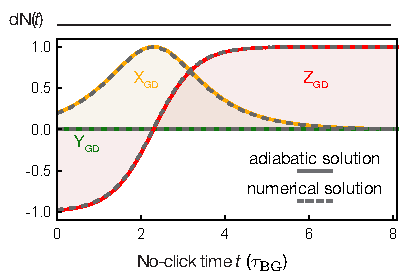
\includegraphics[scale=1.5]{qmjump/knowledge_img1}
\par\end{centering}
\caption[Adiabatic solution for the no-click GD manifold trajectory of a superposition
state measured with $\Odg=0$]{\textbf{\label{fig:3:adiabatic-sol}Adiabatic solution for the no-click
GD manifold trajectory of a superposition state measured with }$\Odg=0$\textbf{.
}Adiabatic-approximation (solid lines) and numerical (dashed lines)
solution for the partial tomogram of the GD manifold of the no-click
quantum trajectory of an initial superposition state $\ket{\psi\left(0\right)}=\mathcal{N}\left(\G+\epsilon\D\right)$,
where $\epsilon=0.1$ and $\mathcal{N}=\left(1+\epsilon^{2}\right)^{-1/2}$.
The Bright Rabi drive is $\Obg=0.1$, in units of the decay rate $\gamma_{{\rm B}}$.
Time axis scaled in units of $\tau_{\mathrm{BG}}=\left(\Obg^{2}/\gamma_{{\rm BG}}\right)^{-1}.$}
\end{figure}
\begin{align}
\cgn\left(t\right)^{2}= & \frac{p_{{\rm G}}}{p_{{\rm G}}+\left(1-p_{{\rm G}}\right)e^{2t/\tau_{{\rm BG}}}}\,,\label{eq:Cgnoclicksol}\\
\cdn\left(t\right)^{2}= & \frac{p_{{\rm D}}e^{t/\tau_{{\rm BG}}}}{p_{{\rm D}}+\left(1-p_{{\rm D}}\right)e^{2t/\tau_{{\rm BG}}}}\,,\label{eq:CdNoClickSol}
\end{align}
where $p_{{\rm G}}\equiv\cgn\left(0\right)^{2}$ and $p_{{\rm D}}\equiv\cdn\left(0\right)^{2}$
are the initial conditions. Note, for $p_{{\rm D}}=0$, the above
solution for $\cdn$ is always zero. The evolution of the GD Bloch
vector conditioned on no clicks for the initial state $\ket{\psi\left(0\right)}=\mathcal{N}\left(\G+\epsilon\D\right)$
is obtained by substituting Eq.~(\ref{eq:Cgnoclicksol}) and (\ref{eq:CdNoClickSol})
in Eqs.~(\ref{eqn:Z})-(\ref{eqn:Y}), 
\begin{align}
{\rm Z}_{{\rm GD}}(t) & ={\rm tanh}\left[t/\tau_{{\rm BG}}+\mathrm{arctanh}\left[{\rm Z}_{{\rm GD}}(0)\right]\right],\label{eq:Zgd-Adi}\\
{\rm X}_{{\rm GD}}(t) & ={\rm sech}\left[t/\tau_{{\rm BG}}+\mathrm{arctanh}\left[{\rm Z}_{{\rm GD}}(0)\right]\right],\\
{\rm Y}_{{\rm GD}}(t) & =0.\label{eq:Ygd-Adi}
\end{align}
We note that a few results of this subsection, especially Eqs.~(\ref{eq:Zgd-Adi})-(\ref{eq:Ygd-Adi}),
bear resemblance to results from Sec.~\ref{sec:thry:3lvl-atom-simple-log},
yet we stress that  the two situations are fundamentally distinct,
and the resemblance must be considered with care. For instance, we
note that the mid-flight time $\Delta t_{\mathrm{mid}}$ cannot be
recovered from the simpler situation considered here, where no quantum
jumps occur and there is no competition between unitary dynamics due
to $\Omega_{{\rm DG}}$ and the measurement. 

In Fig.~\ref{fig:3:adiabatic-sol}a, we plot the adiabatic-approximation
solution to the non-linear Schrödinger evolution, Eq.~(\ref{eq:NL-SSe-Cond-3}),
for the GD manifold Bloch vector conditioned on no clicks, Eqs.~(\ref{eq:Zgd-Adi})-(\ref{eq:Ygd-Adi}),
obtained in the limit $\Obg\ll\gamma_{B}$. Overlaid (dashed lines)
is the corresponding numerically calculated solution to Eq.~(\ref{eq:NL-SSe-Cond-3}).
Even for modest separation of timescales, $\Obg/\gamma_{{\rm B}}=0.1$
in the plot, the two solutions appear nearly indistinguishable. The
initial atom state, $\epsilon=0.1$, is gradually projected to $\D$
on a timescale given by $\tau_{{\rm BG}}$ and evolves in a characteristically
non-unitary manner. Notably, the state remains pure at all times,
and in the limit $t\gg\tau_{{\rm BG}}$ remains essentially in $\D$,
indefinitely. Importantly, for times $t$ on the other of $\tau_{{\rm BG}}$,
the projection can (but need not) be interrupted by the detection
of a click, which would project the state to $\G$, and occurs with
total probability $\approx1-\epsilon^{2}$. 
\begin{figure}
\begin{centering}
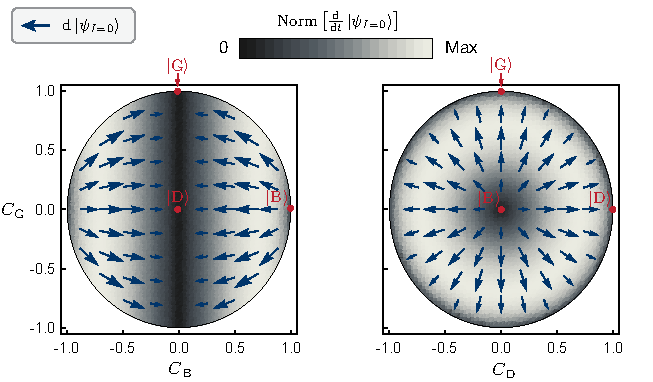
\includegraphics[scale=1.4]{qmjump/knowledge_img2}
\par\end{centering}
\caption[Geometrical representation of the no-click measurement-backaction
force for $\Obg=0$]{\textbf{\label{fig:Knowledge-driven-force-in-1}Geometrical representation
of the no-click measurement-backaction  force for $\Obg=0$.} Shown
are two projections of $\mathbb{\mathbb{\mathbb{R}}}$-qutrit sphere
overlaid with the measurement-force vector field, $\frac{\mathrm{d}}{\mathrm{d}t}\ket{\psi_{I=0}}$,
due to the monitoring of the B level with $\Obg=0$. Color of density
plot indicates the relative magnitude of the change, $\mathrm{Norm}\left[\frac{\mathrm{d}}{\mathrm{d}t}\ket{\psi_{I=0}}\right]$.}
\end{figure}


\paragraph{Hilbert space representation of the measurement dynamics.}

It is useful to consider a geometric representation of the measurement
dynamics and in particular of the non-linear measurement-backaction
force. For simplicity, first consider the measurement force due only
to the monitoring of the B level, in the absence of the Bright Rabi
drive, $\Obg=0$. This  force can be represented as a vector field
on the surface of the $\mathbb{R}$-qutrit sphere, see Fig.~\ref{fig:Knowledge-driven-force-in-1}.
The vector field is calculated from Eqs.~(\ref{eq:Zgd-Adi})-(\ref{eq:Ygd-Adi})
for the change in the state conditioned on detecting no clicks, 
\begin{equation}
\frac{\mathrm{d}}{\mathrm{d}t}\ket{\psi_{I=0}}=\frac{1}{2}\gamma_{{\rm B}}\cbn{}^{2}\begin{pmatrix}\cbn-1\\
\cgn\\
\cdn
\end{pmatrix}\,.\label{eq:ddtPsiI-vec}
\end{equation}
The colormap in Fig.~\ref{fig:Knowledge-driven-force-in-1} depicts
the relative magnitude of the change, $\mathrm{Norm}\left[\frac{\mathrm{d}}{\mathrm{d}t}\ket{\psi_{I=0}}\right],$
which we note is only zero in two special cases: i) when the atom
is $\pm\B$, corresponding to the points $\left(\pm1,0,0\right),$
and ii) when the atom is in a\emph{ }state involving exclusively $\G$
and $\D$ but not $\B$. The latter is special in that it corresponds
to an entire manifold of states, the GD equatorial circle, which can
be visually recognized in Fig.~\ref{fig:Knowledge-driven-force-in-1}
as the dark vertical stripe at the center of the left panel and the
dark circular perimeter of the disk in the right panel. All other
states, not covered under the latter two cases, are superpositions
involving $\B$. From the vector field plot, it is evident that these
states are guided by the force away from the $\B$ poles and toward
the GD equator. It is precisely this feature of the measurement force
that results in the gradual projection of the state conditioned on
no clicks — it is the unavoidable disturbance of the atom due to the
information-gain of the no-click measurement outcomes, which lead
the observer to gradually learn that the atom is not in $\D$, thus
resulting in the increased likelihood that it is in $\G$ or $\D$.
This dynamics embody the message of the Chapter~\ref{chap:Quantum-Trajectory-Theory}
epigraph, ``In quantum physics you don't see what you get, you get
what you see.''

\begin{figure}
\begin{centering}
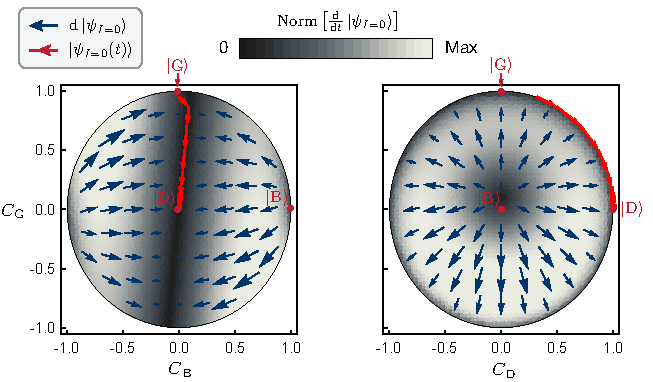
\includegraphics[scale=1.4]{qmjump/knowledge_img3}
\par\end{centering}
\caption[Geometrical representation of the measurement-backaction force and
a no-click trajectory with $\Obg=0.1\gamma_{{\rm B}}$]{\textbf{\label{fig:Knowledge-driven-force-in-2}Geometrical representation
of the measurement-backaction force and a no-click trajectory with
$\Obg=0.1\gamma_{{\rm B}}$.}  Two projections of the $\mathbb{\mathbb{\mathbb{R}}}$-qutrit
sphere overlaid with the measurement-force vector field $\frac{\mathrm{d}}{\mathrm{d}t}\ket{\psi_{I=0}}$
(blue arrows) and the path of the quantum trajectory from Fig.~(\ref{fig:3:adiabatic-sol})
(red arrows), depicting the gradual projection of a superposition
state to $\D$ conditioned on no clicks. Density plot indicates relative
field magnitude, $\mathrm{Norm}\left[\frac{\mathrm{d}}{\mathrm{d}t}\ket{\psi_{I=0}}\right]$.}
\end{figure}

In Fig.~\ref{fig:Knowledge-driven-force-in-2}, we plot the measurement
vector field in the presence of the Bright Rabi drive $\Omega_{\mathrm{BG}}$,
\begin{equation}
\frac{\mathrm{d}}{\mathrm{d}t}\ket{\psi_{I=0}}=\frac{1}{2}\gamma_{{\rm B}}\cbn{}^{2}\begin{pmatrix}\cbn-1\\
\cgn\\
\cdn
\end{pmatrix}+\frac{1}{2}\Obg\begin{pmatrix}\cgn\\
-\cbn\\
0
\end{pmatrix}\,,\label{eq:ddtPsiI-vec-1}
\end{equation}
with $\Obg=0.1\gamma_{{\rm B}}$. The Bright Rabi drive, visually
represented on the $\mathbb{R}$-qutrit sphere in Fig.~\ref{fig:R-qutrit-sphere-representation.},
perturbs the measurement field, shown in Fig.~\ref{fig:Knowledge-driven-force-in-1},
by linking the B and G levels and lifting the degeneracy of the measurement,
represented in GD equator. Visually, this is evident in the tilt of
the vertical dark stripe in the center of the left-panel colormap.
In the right panel, it is also evident that $\B$ is no longer an
equilibrium point; the equilibrium has been shifted in the direction
of $\G$ by an amount proportional $\Obg/\gamma_{{\rm B}},$ see Eq.~(\ref{eq:Cb-bar}),
and made metastable. The red arrows depict the path of the quantum
trajectory in Hilbert of the gradual projection of an initial superposition
state of $\G$ and $\D$, for the same parameters as employed in Fig.~(\ref{fig:3:adiabatic-sol}),
where $\epsilon=0.1$. Initially, the state is quickly steered in
the direction of $\B$ by the force of $\Obg$. However, as the state
moves in the direction of $\B$, the motion is quickly opposed by
the no-click measurement-backaction force, which grows larger in amplitude
in this direction. The two forces do not precisely cancel each other
out, because of the slight mismatch in angles. The net force, albeit
small, steers the atom towards the GD equator and with a slight tilt
toward $\D$. The opposition of the $\Obg$ drive and the measurement
back-action ``trap'' the state in the ridge where the two forces
nearly cancel each other out, the nearly vertical dark stripe in the
left panel, and the small angular mismatch slowly carries the state
in the direction of $\D$, an equilibirum point, where all forces
are zero.


\subsection{Incoherent Bright drive and Dark drive off\label{subsec:Incoherent-Bright-drive}}

In this section, we consider the case of quantum jumps in the three-level
atom subject to photodetection and an incoherent Bright drive, rather
than a Rabi one, see Sec.~\ref{sec:thry:3lvl-atom-simple-log}. The
situation analyzed in this section is somewhat more analogous to the
cQED experiment where the Bright Rabi drive consists of a bi-chromatic
tone that unconditionally addresses the BG transition, independent
of the population of the readout cavity, necessitated by the  dispersive
pull of the readout cavity on the BG frequency. The bi-chromatic drive
effectively acts as an incoherent drive. The incoherent Bright drive
photodetection theory presented here sheds some further light on the
dynamics of the quantum jump from $\G$ to $\D$. Features such as
the non-zero coherence, $X_{{\rm GD}}$, and in the limit $\deltatcatch\gg\Delta t_{{\rm mid}}$
are discussed.\footnote{The following derivation is due to H.J. Carmichael and R. Gutierrez-Jauregui.}

Replacing the coherent Rabi drive $\Omega_{{\rm BG}}$ by an incoherent
drive $\Gamma_{{\rm BG}}$ in  the master equation of the three-level
atom in the interaction picture, Eq.~(\ref{eq:PhotonLindblad}) becomes
\begin{equation}
\frac{\mathrm{d}\rho}{\mathrm{d}t}=(i\hbar)^{-1}[\hat{H}_{{\rm drive}},\rho]+\Gamma_{{\rm BG}}{\cal D}\left[\kb{\rm B}{\rm G}\right]\rho+(\gamma_{{\rm B}}+\Gamma_{{\rm BG}}){\cal D}\left[\kb{\rm G}{\rm B}\right]\rho+\gamma_{{\rm D}}{\cal D}\left[\kb{\rm G}{\rm D}\right]\rho,
\end{equation}
and Eq.~(\ref{eq:ClickHeff}) becomes
\begin{equation}
\hat{H}_{{\rm drive}}=i\hbar\frac{\Omega_{{\rm DG}}}{2}\big(\kb{\rm D}{\rm G}-\kb{\rm G}{\rm D}\big).
\end{equation}
The strong-monitoring assumption, $\tau_{{\rm BG}}^{-1}\ll\gamma_{{\rm B}}$,
is also carried over from Sec.~\ref{sec:thry:3lvl-atom-simple-log}
by assuming $\Gamma_{{\rm BG}}\ll\gamma_{{\rm B}}$, i.e., the time
between clicks in fluorescence is essentially the same as the time
separating photon absorptions from the incoherent drive, as absorption
is rapidly followed by fluorescence ($\gamma_{{\rm B}}+\Gamma_{{\rm BG}}\gg\Gamma_{{\rm BG}}$).
This brings a useful simplification, since, following each reset to
$\G$, the unnormalized state evolves in the GD-subspace, 
\begin{equation}
i\hbar\frac{\mathrm{d}\ket{\tilde{\psi}}}{\mathrm{d}\Delta t_{{\rm catch}}}=\left(\hat{H}_{{\rm drive}}-i\hbar\frac{\Gamma_{{\rm BG}}}{2}\kb{\rm G}{\rm G}-i\hbar\frac{\gamma_{{\rm D}}}{2}\kb{\rm D}{\rm D}\right)\ket{\tilde{\psi}},
\end{equation}
thus replacing Eqs.~(\ref{eqn:3x3_system}) and (\ref{eqn:W_DG_equation_coherent})
by the simpler $2\times2$ system 
\begin{equation}
\frac{\mathrm{d}}{\mathrm{d}\Delta t_{{\rm catch}}}\begin{pmatrix}\cg\\
\cd
\end{pmatrix}=\frac{1}{2}\left(\begin{matrix}-\Gamma_{{\rm BG}} & -\Omega_{{\rm DG}}\\
\Omega_{{\rm DG}} & -\gamma_{{\rm D}}
\end{matrix}\right)\begin{pmatrix}\cg\\
\cd
\end{pmatrix},
\end{equation}
and, in the limit $\gamma_{{\rm D}}\ll\Gamma_{{\rm BG}}$, the equation
of motion for $W_{{\rm DG}}$, defined in Eq.~(\ref{eqn:W_DG_definition}),
is
\begin{equation}
\frac{\mathrm{d}W_{{\rm DG}}}{\mathrm{d}\Delta t_{{\rm catch}}}=\frac{\Gamma_{{\rm BG}}}{2}W_{{\rm DG}}+\frac{\Omega_{{\rm DG}}}{2}(1+W_{{\rm DG}}^{2}),\label{eqn:W_DG_equation_incoherent}
\end{equation}
with solution, for $W_{{\rm DG}}(0)=0$, 
\begin{equation}
W_{{\rm DG}}(\Delta t_{{\rm catch}})=\frac{\exp\left[(V-V^{-1})\Omega_{{\rm DG}}\Delta t_{{\rm catch}}/2\right]-1}{V-V^{-1}\exp\left[(V-V^{-1})\Omega_{{\rm DG}}\Delta t_{{\rm catch}}/2\right]},\label{eqn:W_DG_incoherent}
\end{equation}
where 
\begin{equation}
V=\frac{1}{2}\frac{\Gamma_{{\rm BG}}}{\Omega_{{\rm DG}}}+\sqrt{\frac{1}{4}\left(\frac{\Gamma_{{\rm BG}}}{\Omega_{{\rm DG}}}\right)^{2}-1}.
\end{equation}
In Ref.~\citet{Ruskov2007}, a general form of the Bloch vector equations
for arbitrary amplitude of the Rabi drive was found. Inversion of
the condition $W_{{\rm DG}}(\Delta t_{{\rm mid}})=1$ gives the characteristic
time scale 
\begin{equation}
\Delta t_{{\rm mid}}=2\left[(V-V^{-1})\Omega_{{\rm DG}}\right]^{-1}\ln\left(\frac{V+1}{V^{-1}+1}\right).\label{eqn:t_mid_incoherent}
\end{equation}
Although Eqs.~(\ref{eqn:W_DG_incoherent}) and (\ref{eqn:t_mid_incoherent})
replace Eqs.~(\ref{eq:WDG-coh}) and (\ref{eq:t_mid_coherent}),
under strong monitoring, $\Gamma_{{\rm BG}}\gg\Omega_{{\rm DG}}$,
they revert to the latter with the substitution $\Omega_{{\rm BG}}^{2}/2\gamma_{{\rm B}}\to\Gamma_{{\rm BG}}/2$,;
in this way, Eqs.~(\ref{eqn:Z})–(\ref{eqn:Y}) are recovered with
the same substitution. More generally, $W_{{\rm DG}}(\Delta t_{{\rm catch}})$
goes to infinity at finite $\Delta t_{{\rm catch}}$, changes sign,
and returns from infinity to settle on the steady value $W_{{\rm DG}}(\infty)=-V$.
The singular behavior marks a trajectory passing through the north
pole of Bloch sphere. It yields the long-time solution 
\begin{equation}
{\rm Z}_{{\rm GD}}(\infty)=\sqrt{1-4\left(\frac{\Omega_{{\rm DG}}}{\Gamma_{{\rm BG}}}\right)^{2}},\qquad{\rm X}_{{\rm GD}}(\infty)=-2\frac{\Omega_{{\rm DG}}}{\Gamma_{{\rm BG}}},\qquad{\rm Y}_{{\rm GD}}(\infty)=0,\label{eq:ZGDXGD-long-term}
\end{equation}
in contrast to the perfect jump of Eqs.~(\ref{eqn:Z_approx})–(\ref{eqn:Y_approx}).
The long-term coherence and lower-than-one value of Z were observed
in the experiments, see Fig.~\ref{fig:catch}b. They can be understood
as the equilibrium point of the coherent Rabi drive $\Omega_{{\rm DG}}$
attempting to rotate the state from $\D$ back to $\G$ perfectly
balanced against the measurement-backaction force of the no-click
measurement steering the atom toward $\D$, recall discussion of the
measurement vector field, see Figs.~\ref{fig:Knowledge-driven-force-in-1}
and~\ref{fig:Knowledge-driven-force-in-2}. 

\paragraph{\textit{\emph{Dark drive off.}}}

Turing the Dark drive off shortly after a click demonstrates the connection
between the flight of a quantum jump and a projective measurement.
From the point of view of the trajectory equations, the only change
is the setting of $\Omega_{{\rm DG}}$ to zero at time $\Delta t_{{\rm on}}$
on the right-hand side of Eqs.~(\ref{eqn:W_DG_equation_coherent})
and (\ref{eqn:W_DG_equation_incoherent}). Subsequently, $W_{{\rm DG}}(\Delta t_{{\rm catch}})$
continues its exponential growth at rate $\Omega_{{\rm BG}}^{2}/2\gamma_{B}$
{[}Eq.~(\ref{eqn:W_DG_equation_coherent}){]} or $\Gamma_{{\rm BG}}/2$
{[}Eq.~(\ref{eqn:W_DG_equation_incoherent}){]}. Equations (\ref{eqn:Z})–(\ref{eqn:Y})
for the GD Bloch components still hold, but now with 
\begin{equation}
\Delta t_{{\rm mid}}=\left(\frac{\Omega_{{\rm BG}}^{2}}{2\gamma_{B}},\frac{\Gamma_{{\rm BG}}}{2}\right)^{-1}\ln\big[W_{{\rm DG}}^{-2}(\Delta t_{{\rm on}})\big].
\end{equation}
which can provide an estimate of $\Delta t'_{\mathrm{mid}}$, specifying
the time at which $Z_{\mathrm{GD}}=0$.

The evolution during $\Delta t_{\mathrm{off}}$, in the absence of
$\Omega_{\mathrm{DG}}$, in effect realizes a projective measurement
of whether the state of the atom is $\G$ or $|{\rm D}\rangle$, similar
to the one analyzed in Sec.~\ref{subsec:Knowledge-driven-force-in},
where the normalized state at $\Delta t_{{\rm on}}$ is 
\begin{equation}
\frac{|\psi(\Delta t_{{\rm on}})\rangle}{\sqrt{\mathcal{N}(\Delta t_{{\rm on}})}}=\frac{\cg(\Delta t_{{\rm on}})\G+\cd(\Delta t_{{\rm on}})\D}{\sqrt{\mathcal{N}(\Delta t_{{\rm on}})}},\label{eqn:initial_state}
\end{equation}
with $\mathcal{N}(\Delta t_{{\rm on}})=\cg^{2}(\Delta t_{{\rm on}})+\cd^{2}(\Delta t_{{\rm on}})$
the probability for the jump to reach $\Delta t_{{\rm catch}}=\Delta t_{{\rm on}}$
after a click reset to $\G$ at $\Delta t_{{\rm catch}}=0$. The probability
for the jump to continue to $\Delta t_{{\rm catch}}>\Delta t_{{\rm on}}$
(given $\Delta t_{{\rm on}}$ is reached) is then 
\begin{equation}
\frac{\mathcal{N}(\Delta t_{{\rm catch}})}{\mathcal{N}(\Delta t_{{\rm on}})}=\frac{C_{{\rm D}}^{2}(\Delta t_{{\rm on}})}{\mathcal{N}(\Delta t_{{\rm on}})}+\frac{C_{{\rm G}}^{2}(\Delta t_{{\rm on}})}{\mathcal{N}(\Delta t_{{\rm on}})}\exp\left[-\left(\frac{\Omega_{{\rm BG}}^{2}}{\gamma_{{\rm B}}},\Gamma_{{\rm BG}}\right)\Delta t_{{\rm catch}}\right].\label{eq:completion-prob}
\end{equation}


\paragraph{Completed and aborted evolutions of the jump transition.}

In this simple model, the probability for the trajectory to complete
— for the measurement to yield the result $|{\rm D}\rangle$ — is
obtained in the limit $\Delta t_{\mathrm{catch}}\rightarrow\infty$,
and, as expected, is equal to the probability to occupy the state
$|{\rm D}\rangle$ at time $\Delta t_{{\rm on}}$; i.e., the completion
probability is $P_{\mathrm{D}}(\Delta t_{{\rm on}})=C_{{\rm D}}^{2}(\Delta t_{{\rm on}})/{{\rm Norm}(\Delta t_{{\rm on}})}$.
It is helpful to illustrate this idea with an example. Consider the
catch experiment of Fig.~\ref{fig:catch}b in the absence of the
Dark Rabi drive, $\Omega_{\mathrm{DG}}$. From $Z_{\mathrm{GD}}$,
we can estimate that out of all the trajectories that pass though
the $\Delta t_{{\rm on}}$ mark approximately $P_{\mathrm{D}}(\Delta t_{{\rm on}})=(1+Z_{\mathrm{GD}}(\Delta t_{{\rm on}}))/2\approx8\%$
fully complete without an interruption. On the other hand, for those
that pass the $\Delta t'_{\mathrm{mid}}$ mark, approximately 50\%
complete. It follows from Eq.~(\ref{eq:completion-prob}), that the
probability of the evolution to complete increases the further along
the trajectory is. Although some of the jump evolutions abort at random,
importantly, every single jump evolution that completes, and is thus
recorded as a jump, follows \textit{not} a random but an identical
path in Hilbert space, i.e., a deterministic one. This path (of \textit{any}
jump) is determined by Eq.~(\ref{eqn:W_DG_incoherent}), or, in the
simpler model, by the Eqs.~(\ref{eqn:Z_approx})-(\ref{eqn:Y_approx})
for the components of the GD Bloch vector.

\section{Heterodyne monitoring of readout cavity coupled to three-level atom\label{sec:Heterodyne-monitoring-of}}

\subsection{Description of cQED experiment \label{subsec:Description-of-cQED}}

In Chapter 1, we described the cQED experiment  involving a superconducting
atom with the necessary V-shape level structure (see Fig.~\ref{fig:setup}a
or Sec.~\ref{sec:circuit-design}) subject to heterodyne monitoring
of $\B$ by means a dispersively coupled readout cavity. The three-level
atom is formed form two heavily hybridized transmon modes, which are
coupled by means of a cross-Kerr interaction to the readout cavity
in an asymmetric way, $\chi_{\mathrm{BC}}\gg\chi_{\mathrm{DC}}$.
In the following, we present the quantum trajectory description of
the heterodyne monitoring, including imperfections.

\paragraph{System Hamiltonian. }

In the lab frame, the Hamiltonian of the system is, see also Sec.~\ref{sec:circuit-design},
\begin{equation}
\hat{H}_{{\rm lab}}=\hat{H}_{0}+\hat{H}_{I}+\hat{H}_{d}\left(t\right)\,,
\end{equation}
where the Hamiltonian of the uncoupled three-level atom and cavity,
is 
\begin{equation}
\hat{H}_{0}=\hbar\omega_{{\rm DG}}\kb{\rm D}{\rm D}+\hbar\omega_{{\rm BG}}\kb{\rm B}{\rm B}+\hbar\omega_{C}\hat{c}^{\dagger}\hat{c}\,,
\end{equation}
where $\omega_{{\rm DG}}$, $\omega_{{\rm BG}}$, $\omega_{{\rm C}}$
are the Dark, Bright, and cavity mode frequency, respectively, $\hat{c}$
is the cavity amplitude operator, the atom-cavity interaction Hamiltonian
is 
\begin{equation}
\hat{H}_{I}=\hat{c}^{\dagger}\hat{c}\left[\hbar\chi_{{\rm B}}\kb{\rm B}{\rm B}+\hbar\chi_{{\rm D}}\kb{\rm D}{\rm D}\right]\:,
\end{equation}
where the shift of the cavity frequency conditioned on $\B$ ($\D$)
is $\chi_{{\rm B}}$ ($\chi_{{\rm D}}$), and the Hamiltonian of the
atom Rabi drives and readout probe tone is
\begin{align}
\hat{H}_{d}\left(t\right)= & -\frac{i\hbar}{2}\left[\kappa\sqrt{\bar{n}}\hat{c}e^{i\left(\omega_{{\rm C}}+\Delta_{{\rm R}}\right)t}+\Omega_{{\rm DG}}^{*}e^{i\left(\omega_{{\rm DG}}+\Delta_{{\rm DG}}\right)t}\kb{\rm G}{\rm D}\right.\nonumber \\
 & \left.+\Omega_{{\rm B0}}^{*}e^{i\omega_{{\rm BG}}t}\kb{\rm G}{\rm B}+\Omega_{{\rm B1}}^{*}e^{i\left(\omega_{{\rm BG}}+\Delta_{{\rm B1}}\right)t}\kb{\rm G}{\rm B}+\mathrm{H.c.}\right]\,,
\end{align}
where $\bar{n}$ is the steady state number of photons in the cavity
when driven resonantly, $\Delta_{{\rm R}}$, $\Delta_{{\rm DG}},$
and $\Delta_{{\rm B1}}$ are the drive detunings from the bare mode
frequencies. The first Bright Rabi tone, $\Omega_{{\rm B0}}$, addresses
the Bright transition when the cavity is unpopulated, while the second
tone, $\Omega_{{\rm B0}}$, addresses the BG transition  when the
cavity is populated, see frequency spectrum in Fig.~\ref{fig:setup}c.
Moving to the rotating frame at the drive frequencies, defined by
the ket transformation $\ket{\psi(t)}=U(t)\ket{\psi_{\mathrm{lab}}(t)}$,
where $U(t)=\exp\left(u\left(t\right)/i\hbar\right)$ and $u(t)=\hbar t\left[\left(\omega_{{\rm C}}+\Delta_{{\rm R}}\right)a^{\dagger}a+\omega_{{\rm BG}}\ket{\rm B}\bra{\rm B}+\left(\omega_{{\rm DG}}+\Delta_{{\rm DG}}\right)\ket{\rm D}\bra{\rm D}\right]$,
the Hamiltonian in the rotating frame is
\begin{equation}
\hat{H}\left(t\right)=\hat{H}_{{\rm R}}+\hat{H}_{{\rm drive}}\left(t\right)\,,
\end{equation}
where $\hat{H}_{\mathrm{R}}$ is a time-independent Hamiltonian,
\begin{equation}
\hat{H}_{{\rm R}}=-\hbar\Delta_{{\rm R}}\hat{c}^{\dagger}\hat{c}+i\hbar\frac{\kappa}{2}\sqrt{\bar{n}}(\hat{c}^{\dagger}-\hat{c})+\hbar\big(\chi_{{\rm B}}\kb{\rm B}{\rm B}+\chi_{{\rm D}}\kb{\rm D}{\rm D}\big)\hat{c}^{\dagger}\hat{c},
\end{equation}
and $\hat{H}_{{\rm drive}}$ is the time-dependent Hamiltonian of
the atom Rabi drives, 
\begin{equation}
\hat{H}_{{\rm drive}}\left(t\right)=i\hbar\left[\frac{\Omega_{{\rm BG}}(t)}{2}\kb{\rm B}{\rm G}-\frac{\Omega_{{\rm BG}}^{*}(t)}{2}\kb{\rm G}{\rm B}\right]+i\hbar\frac{\Omega_{{\rm DG}}}{2}\left(\kb{\rm D}{\rm G}-\kb{\rm G}{\rm D}\right).
\end{equation}
The bi-chromatic drive, which unselectively addresses the BG transition,
$\Omega_{{\rm BG}}(t)=\Omega_{{\rm B}0}+\Omega_{{\rm B}1}\exp(-i\Delta_{{\rm B}1}t)$
replaces the Rabi drive $\Omega_{{\rm BG}}$ of Eq.~(\ref{eq:drive_coherent_fluorescence}).

\paragraph{Measurement record.}

The readout cavity input-output coupling is given by the jump operator
$\sqrt{\kappa}\hat{c}$. It follows from Eq.~(\ref{eq:dJimperf:het})
that the heterodyne measurement-record increment is
\begin{equation}
\mathrm{d}J_{\mathrm{het}}\left(t\right)=\sqrt{\eta\kappa}\left\langle \hat{c}\right\rangle \left(t\right)\dt+\dZ\left(t\right)\,,\label{eq:Record}
\end{equation}
where $\dZ$ is a complex Wiener increment, see discussion below Eq.~(\ref{eq:Jhet-perfect}),
and $\eta$ is the quantum efficiency of the readout and amplification
chain. The record, $\mathrm{d}J_{\mathrm{het}}\left(t\right)$, is
scaled — to units of (readout cavity photon number)$^{1/2}$ — and
filtered to generate the simulated quadratures $I_{{\rm rec}}$ and
$Q_{{\rm rec}}$ of the measurement record: 
\begin{eqnarray}
dI_{{\rm rec}} & = & -\frac{\kappa_{{\rm filter}}}{2}\left[I_{{\rm rec}}dt-\left(\eta\frac{\kappa}{2}\right)^{-1/2}{\rm Re}(\mathrm{d}J_{\mathrm{het}})\right],\label{eqn:simulated_I_int}\\
dQ_{{\rm rec}} & = & -\frac{\kappa_{{\rm filter}}}{2}\left[Q_{{\rm rec}}dt-\left(\eta\frac{\kappa}{2}\right)^{-1/2}{\rm Im}(\mathrm{d}J_{\mathrm{het}})\right],\label{eqn:simulated_Q_int}
\end{eqnarray}
where $\kappa_{{\rm filter}}$ is the bandwidth of the amplifier chain.
In practice, it is assured that $\kappa_{{\rm filter}}$ is the fastest
rate in the problem, $\kappa_{{\rm filter}}\gg\kappa$, so that its
effect is largely negligible.  

\subsection{Simulation of Stochastic Schrödinger equation (SSE) \label{subsec:Simulation-of-linear}}

The quantum trajectory unraveling monitors the reflected probe with
efficiency $\eta$ and accounts for residual photon loss through random
jumps. It follows that the linear stochastic Schrödinger equation
combines a continuous evolution (heterodyne readout channel), 
\begin{equation}
{\rm d}\ket{\psi\left(t\right)}=\left[\frac{1}{i\hbar}\left(\hat{H}_{{\rm drive}}+\hat{H}_{{\rm R}}-i\hbar\frac{\kappa}{2}\hat{c}^{\dagger}\hat{c}\right)\dt+\sqrt{\eta\kappa}\mathrm{d}J_{\mathrm{het}}^{*}\left(t\right)\hat{c}\right]\ket{\psi\left(t\right)},\label{eqn:SSE_continuous}
\end{equation}
with the point-like process (photon loss), 
\begin{equation}
\ket{\psi}\to\hat{c}\ket{\psi}\qquad\text{at rate}\qquad(1-\eta)\kappa\frac{\braOket{\psi}{\hat{c}^{\dagger}\hat{c}}{\psi}}{\braket{\psi}{\psi}}.
\end{equation}
Note that for perfect quantum efficiency, $\eta=1$, the rate of the
photon loss channel goes to zero. We emphasize that expectation values
are performed over the normalized state; importantly, when calculating
the measurement record increment $\mathrm{d}J_{\mathrm{het}}^{*}\left(t\right)$,
see Eq.~(\ref{eq:Record}), $\left\langle \hat{c}\right\rangle \left(t\right)=\braOket{\psi\left(t\right)}{\hat{c}}{\psi\left(t\right)}/\braket{\psi\left(t\right)}{\psi\left(t\right)}.$

\paragraph{\textit{\emph{Independently measured imperfections.}}\emph{ }}

To more realistically model the cQED experiment, we need to account
for the small experimental non-idealities associated with the device
performance; namely, the finite energy relaxation lifetime of the
levels ($T_{1}$), the finite dephasing time of the levels ($T_{2}^{*}$),
which is generally smaller than the bound imposed by the lifetime,
$T_{2}^{*}<T_{1}$, and the finite temperature of the device ($n_{{\rm th}}$).
Specifically, we supplement the stochastic Schrödinger equation by
spontaneous and thermal jumps on both the $\G$ to $\B$ and $\G$
to $\D$ transitions ($n_{{\rm th}}^{{\rm B}}$ and $n_{{\rm th}}^{{\rm D}}$)
and by pure dephasing of the ${\rm GB}$ and ${\rm GD}$ coherences
($\gamma_{{\rm B}}^{\phi}$ and $\gamma_{{\rm D}}^{\phi}$). With
these processes included, the term 
\[
-i\hbar\left\{ \left[\frac{\gamma_{{\rm B}}}{2}(n_{{\rm th}}^{{\rm B}}+1)+\gamma_{{\rm B}}^{\phi}\right]\kb{\rm B}{\rm B}+\left[\frac{\gamma_{{\rm D}}}{2}(n_{{\rm th}}^{{\rm D}}+1)+\gamma_{{\rm D}}^{\phi}\right]\kb{\rm D}{\rm D}+\frac{\gamma_{{\rm B}}n_{{\rm th}}^{{\rm B}}+\gamma_{{\rm D}}n_{{\rm th}}^{{\rm D}}}{2}|\kb{\rm G}{\rm G}\right\} 
\]
is added to the non-Hermitian Hamiltonian, $\hat{H}_{{\rm drive}}+\hat{H}_{{\rm R}}-i\hbar\frac{\kappa}{2}\hat{c}^{\dagger}\hat{c}$,
on the right-hand side of Eq.~(\ref{eqn:SSE_continuous}), with the
additional three point-processes: 
\begin{align}
|\psi\rangle\to|{\rm G}\rangle & \quad\text{at rate}\quad\gamma_{{\rm B}}(n_{{\rm th}}^{{\rm B}}+1)\frac{\langle\psi|{\rm B}\rangle\langle{\rm B}|\psi\rangle}{\langle\psi|\psi\rangle}+\gamma_{{\rm D}}(n_{{\rm th}}^{{\rm D}}+1)\frac{\langle\psi|{\rm D}\rangle\langle{\rm D}|\psi\rangle}{\langle\psi|\psi\rangle},\\
\noalign{\vskip4pt}|\psi\rangle\to|{\rm B}\rangle & \quad\text{at rate}\quad\gamma_{{\rm B}}n_{{\rm th}}^{{\rm B}}\frac{\langle\psi|{\rm G}\rangle\langle{\rm G}|\psi\rangle}{\langle\psi|\psi\rangle}+2\gamma_{{\rm B}}^{\phi}\frac{\langle\psi|{\rm B}\rangle\langle{\rm B}|\psi\rangle}{\langle\psi|\psi\rangle},\\
\noalign{\vskip4pt}|\psi\rangle\to|{\rm D}\rangle & \quad\text{at rate}\quad\gamma_{{\rm D}}n_{{\rm th}}^{{\rm D}}\frac{\langle\psi|{\rm G}\rangle\langle{\rm G}|\psi\rangle}{\langle\psi|\psi\rangle}+2\gamma_{{\rm D}}^{\phi}\frac{\langle\psi|{\rm D}\rangle\langle{\rm D}|\psi\rangle}{\langle\psi|\psi\rangle}.
\end{align}
In the simulation, the parameters $\gamma_{{\rm B,D}}$, $n_{{\rm th}}^{{\rm B,D}}$,
and $\gamma_{{\rm B,D}}^{\phi}$ are mapped to the independently measured
parameters $T_{{\rm B,D}}^{1}$, $n_{{\rm th}}^{{\rm G,D}}$, and
$T_{2{\rm R}}^{{\rm B,D}}$ listed in Table \ref{fig:T1-vs-nbar}.

\paragraph{\textit{\emph{Leakage from the }}\emph{GBD}\textit{\emph{-manifold.}}\emph{ }}

Because the three-level atom is realized from two transmon qubits,
the three-state manifold, $\left\{ \G,\B,\D\right\} $, is not strictly
closed, and transitions to higher excited states are sometimes observed.
This imperfection is modeled in the SSE simulation with the addition
of the further term 
\[
-i\hbar\left\{ \frac{\gamma_{{\rm FG}}}{2}|{\rm G}\rangle\langle{\rm G}|+\frac{\gamma_{{\rm FD}}}{2}|{\rm D}\rangle\langle{\rm D}|+\frac{\gamma_{{\rm GF}}+\gamma_{{\rm DF}}}{2}|{\rm F}\rangle\langle{\rm F}|\right\} 
\]
to the non-Hermitian Hamiltonian, and the associated additional random
jumps, 
\begin{eqnarray}
|\psi\rangle\to|{\rm F}\rangle &  & \qquad\hbox{at\ rate}\qquad\gamma_{{\rm FG}}\frac{\langle\psi|{\rm G}\rangle\langle{\rm G}|\psi\rangle}{\langle\psi|\psi\rangle}+\gamma_{{\rm FD}}\frac{\langle\psi|{\rm D}\rangle\langle{\rm D}|\psi\rangle}{\langle\psi|\psi\rangle},\\
\noalign{\vskip4pt}|\psi\rangle\to|{\rm G}\rangle &  & \qquad\hbox{at\ rate}\qquad\gamma_{{\rm GF}}\frac{\langle\psi|{\rm F}\rangle\langle{\rm F}|\psi\rangle}{\langle\psi|\psi\rangle},\\
\noalign{\vskip4pt}|\psi\rangle\to|{\rm D}\rangle &  & \qquad\hbox{at\ rate}\qquad\gamma_{{\rm DF}}\frac{\langle\psi|{\rm F}\rangle\langle{\rm F}|\psi\rangle}{\langle\psi|\psi\rangle},\label{eqn:jumps_to_F}
\end{eqnarray}
where $|{\rm F}\rangle$ models the all higher level by a single catch-all
higher excited state. The results of the simulation are presented
in Sec.~\ref{subsec:Comparison-between-theory}.


\newpage
\section*{Methods}
\subsection*{Experimental setup}

The Large Hadron Collider (LHC) is the world’s highest-energy particle accelerator and is situated approximately 100\,m underground, close to Geneva, Switzerland. The collider accelerates two counter-rotating beams of protons, guided by superconducting magnets located around a 27\,km circular tunnel, and brings them into collision at four interaction points that house large detectors. The LHCb experiment~\cite{Alves:2008zz,LHCb-DP-2014-002} is instrumented in the region covering the polar angles between 10 and 250\,mrad around the proton beam axis, in which the products from $B$-hadron decays can be efficiently captured and identified. The detector includes a high-precision tracking system with a dipole magnet, providing measurements of momentum and impact parameter (IP), defined for charged particles as the minimum distance of a track to a primary proton-proton interaction vertex (PV). Different types of charged particles are distinguished using information from two ring-imaging Cherenkov (RICH) detectors, a calorimeter and a muon system~\cite{LHCb-DP-2014-002, LHCb-DP-2014-001, LHCb-DP-2013-003,LHCb-DP-2013-001,LHCb-DP-2012-003,LHCb-DP-2012-002}. 

Since the associated data storage and analysis costs would be prohibitive, the experiment does not record all collisions. 
Only potentially interesting events, selected using real-time event filters referred to as triggers, are recorded.
% Instead, a subset of interesting events are isolated for further study using real-time event filters known as triggers. 
The LHCb trigger system has a hardware stage, based on information from the calorimeter and muon systems; followed by a software stage that uses all the information from the detector, including the tracking, to make the final selection of events to be recorded for subsequent analysis. The trigger selection algorithms are based on identifying key characteristics of $B$ hadrons and their decay products, such as high \pt final state particles, and a decay vertex that is significantly displaced from any of the PVs in the event.

For the \RK measurement, candidate events are  required to have passed a hardware trigger algorithm that selects either a high \pt muon; or an electron, hadron or photon with high transverse energy deposited in the calorimeters. The \BuKmm and \BuJpsiKmm candidates must be triggered by one of the muons, whereas \BuKee and \BuJpsiKee candidates must be triggered in one of three ways: by either one of the electrons; by the kaon from the \Bp decay; or by particles in the event that are not decay products of the \Bp candidate. In the software trigger, the tracks of the final-state particles are required to form a displaced vertex with good fit quality. A multivariate algorithm is used for the identification of displaced vertices consistent with the decay of a $B$ hadron~\cite{BBDT, LHCb-PROC-2015-018}.

\subsection*{Analysis description}

The analysis technique used to obtain the results presented in this article is essentially identical to that used to obtain the previous LHCb \RK measurement, described in Ref.~\cite{LHCb-PAPER-2019-009} and only the main analysis steps are reviewed here. 

\subsubsection*{Event selection} 

Kaon and muon candidates are identified using the output of multivariate classifiers that exploit information from the tracking system, the RICH detectors, the calorimeters and the muon chambers.
Electrons are identified by matching tracks to  particle showers in the electromagnetic calorimeter~(ECAL) and using the ratio of the energy detected in the ECAL to the momentum measured by the tracking system. 
An electron that emits a bremsstrahlung photon due to interactions with the material of the detector downstream of the dipole magnet results in the photon and electron depositing their energy in the same ECAL cells, and therefore in a correct measurement of the original energy of the electron in the ECAL. However, a bremsstrahlung photon emitted upstream of the magnet  will deposit energy in a different part of the ECAL than the electron, which is deflected in the magnetic field. For each electron track, a search is therefore made in the ECAL for energy deposits around the extrapolated track direction before the magnet that are not associated with any other charged tracks. The energy of any such deposit is added to the electron energy that is derived from the measurements made in the tracker. Bremsstrahlung photons can be added to none, either, or both of the final-state \ep and \en candidates. 

In order to suppress background, each final-state particle is required to have sizeable \pt and to be inconsistent with coming from a PV. The particles are required to originate from a common vertex, with good vertex-fit quality, that is displaced significantly from all of the PVs in the event. The PVs are reconstructed by searching for space points where an accumulation of track trajectories is observed. A weighted least-squares method is then employed to find the precise vertex position. The \Bp momentum vector is required to be aligned with the vector connecting one of the PVs in the event (below referred to as the associated PV) and the \Bp decay vertex. The value of \qsq is calculated using only the lepton momenta, without imposing any constraint on the \mKll mass. 

The \mKll mass ranges and the \qsq regions used to select the different decay modes are shown in Table~\ref{tab:q2ranges}. The selection requirements applied to the nonresonant and resonant decays are otherwise identical. For the muon modes, the superior mass resolution allows a fit in a reduced \mKll mass range compared to the electron modes. For the electron modes, a wider mass region is needed to perform an accurate fit, but the range chosen suppresses any significant contribution from $B\to\Kp\pi\pi\epem$ decays. The residual contribution from such decays is considered as a source of systematic uncertainty. Resolution effects similarly motivate the choice of nonresonant \qsq regions, with a lower limit that excludes contributions from $\phi$-meson decays and an upper limit that reduces the tail from \BuJpsiKee decays.

\begin{table}[t]
\centering
\caption{Nonresonant and resonant mode $\qsq$ and \mKll ranges. The variables \mKll and \mKllconst are used for nonresonant and resonant decays, respectively.}\label{tab:q2ranges}
\begin{tabular}{ccc}
\toprule
Decay mode & \qsq & \mKllgeneric \\
           & $[\gevgevcccc]$ & $[\gevcc]$ \\
\midrule
{\begin{tabular}{r@{\;}l}nonresonant&$e^+e^-$\\resonant&$e^+e^-$\\nonresonant&$\mu^+\mu^-$\\resonant&$\mu^+\mu^-$\end{tabular}}     & {\begin{tabular}{r@{.}l@{\;--\;}r@{.}l}1&1 & 6&0\\6&00 & 12&96\\1&1 & 6&0\\8&68&10&09\end{tabular}}    & {\begin{tabular}{r@{\;--\;}l}4.88&6.20\\5.08&5.70\\5.18&5.60\\5.18&5.60\end{tabular}}\\
\bottomrule
\end{tabular}
\end{table}

Cascade background of the form \HbtoHc, where 
% \Hb is a hadron containing a \bquark quark (\Bu, \Bz, \Bs or \Lb), 
\Hc is a hadron containing a \cquark quark (\Dz, \Dp, \Ds, \Lc), and $X$, $Y$ are particles that are not included in the \Bu candidate, are suppressed by requiring that the kaon-lepton invariant mass is in the region \mbox{$m(\Kp\ellm)>m_{\Dz}$}, where $m_{\Dz}$ is the known $\Dz$ mass~\cite{PDG2020}. Analogous background sources with a misidentified particle are reduced by applying a similar veto, but with the lepton-mass hypothesis changed to that of a pion (denoted $\ell_{[\to\pi]}$). In the muon case, $K\mu_{[\to \pi]}$ combinations with a mass smaller than $m_{\Dz}$ are rejected. In the electron case, a $\pm40\mevcc$ window around the \Dz mass is used to reject candidates where the veto is applied without the bremsstrahlung recovery, \ie  based on only the measured track momenta. The mass distributions are shown in Fig.~\ref{fig:cascadeVeto}.  The veto requirements retain 97\% of \BuKmm and 95\% of \BuKee decays passing all other selection requirements. 

\begin{figure}[!tb]
   \begin{center}
      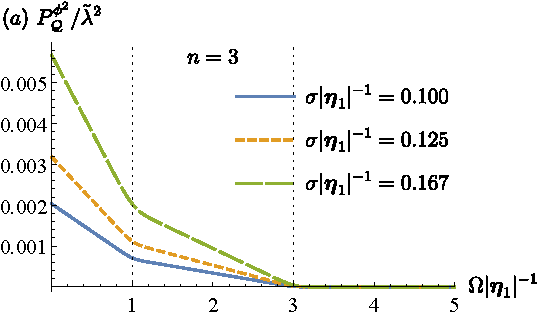
\includegraphics[width=0.48\linewidth]{figures/Fig5a.pdf}
      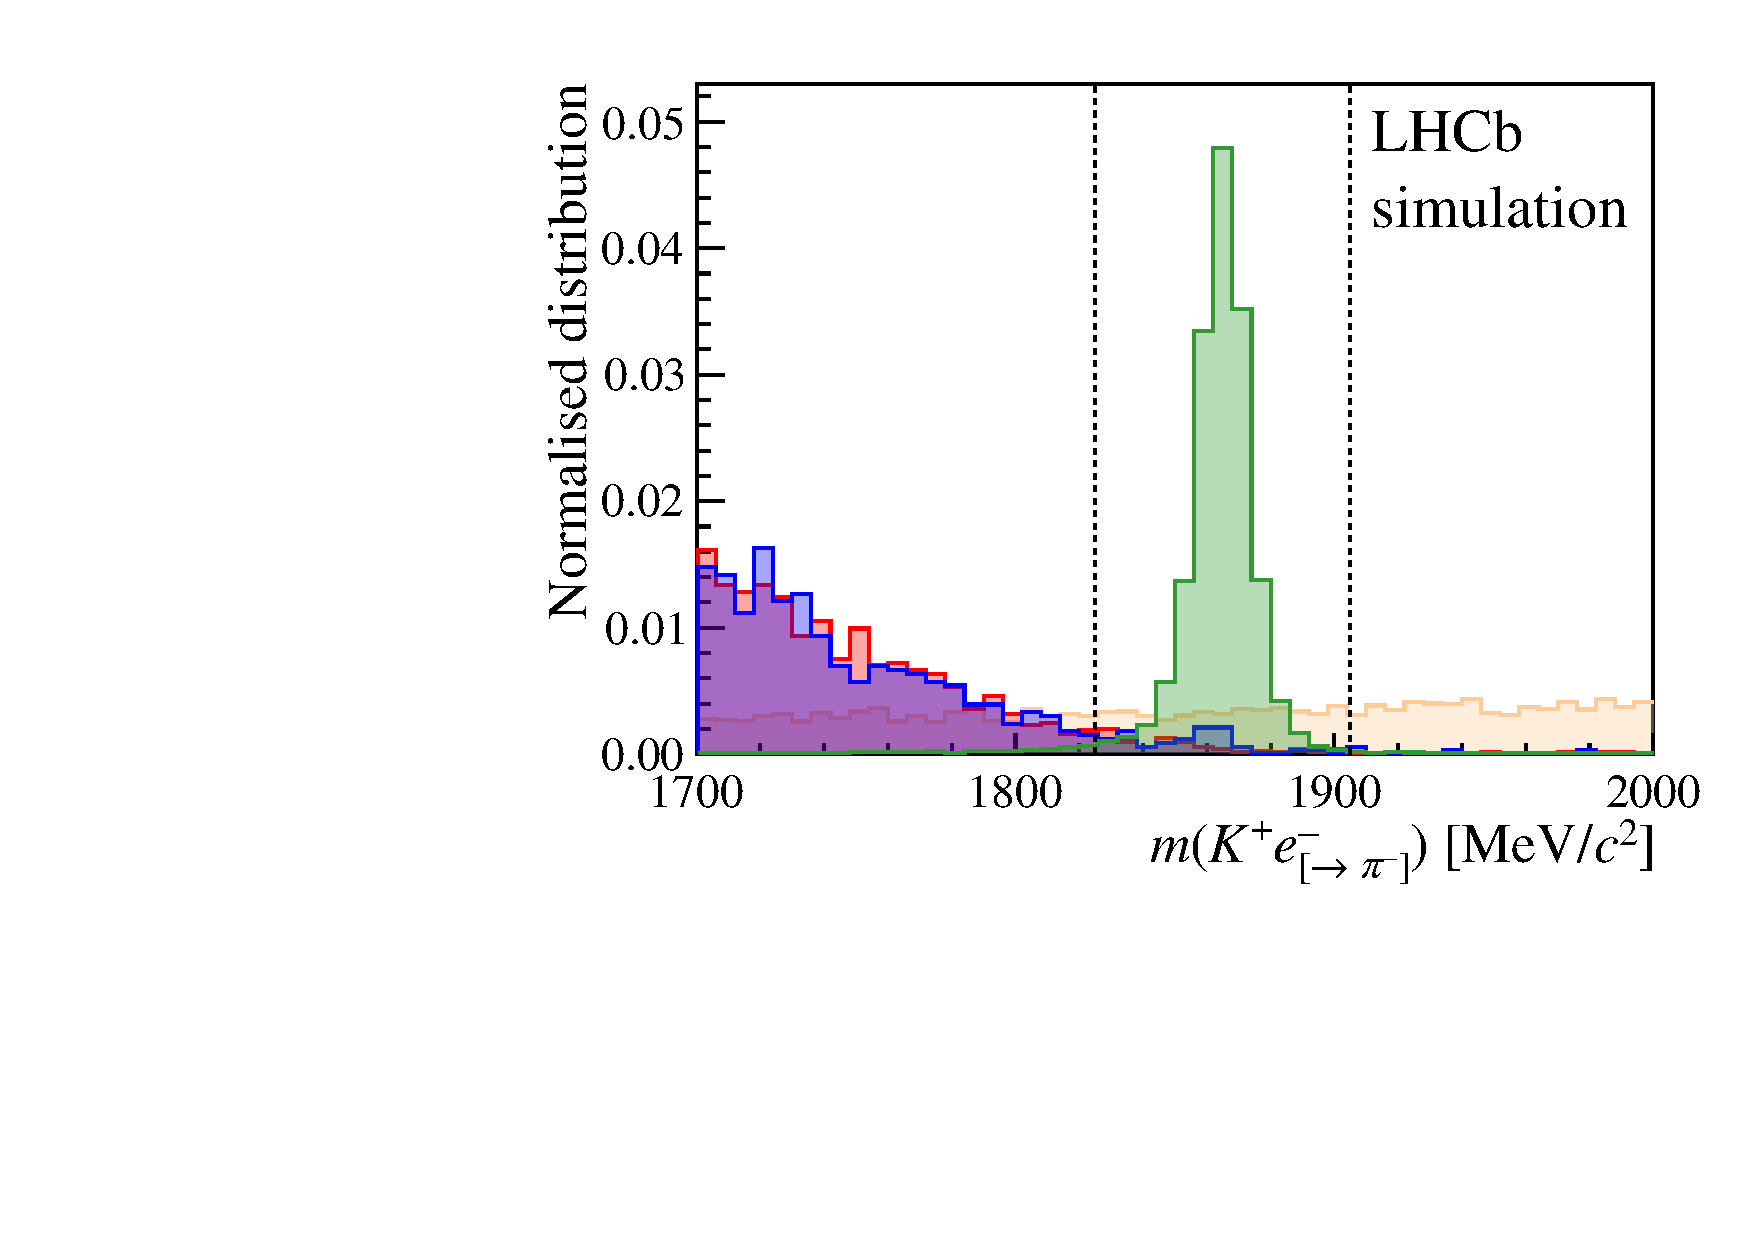
\includegraphics[width=0.48\linewidth]{figures/Fig5b.pdf}
   \end{center}
    \vspace*{-0.5cm}
   \caption{Simulated $K^+e^-$ mass distributions for  signal and various cascade background samples. The distributions are all normalised to unity.  (Left, with log $y$-scale)
   the bremsstrahlung correction to the momentum of the electron is applied, resulting in a tail to the right. The region to the left of the vertical dashed line is rejected. (Right, with linear $y$-scale) the mass is computed only from the track information. The notation $\pi^-_{[\rightarrow e^-]}$ ($e^-_{[\rightarrow \pi^-]}$) is used to denote an electron (pion) that is misidentified as a pion (electron). The region between the dashed vertical lines is rejected. }\label{fig:cascadeVeto}
\end{figure}

Background from other exclusive $B$-hadron decays requires at least two particles to be misidentified. These include the decays \BuKpipi, and misreconstructed \BuJpsiKll and \BuPsiKll decays. In the latter two decays the kaon is misidentified as a lepton and the lepton (of the same electric charge) as a kaon. Such background is reduced to a negligible level by particle-identification criteria. Background from decays with a photon converted into an \epem pair are also negligible due to the \qsq selection.


\subsubsection*{Multivariate selection}

A Boosted Decision Tree (BDT)  algorithm~\cite{Breiman} with gradient boosting~\cite{GradBoost} is used to reduce combinatorial background. For the nonresonant muon mode and for each of the three different trigger categories of the 
nonresonant electron mode, a single BDT classifier is trained for the 7 and $8\tev$ data, and an additional classifier is trained for the $13\tev$ data. The BDT output is not strongly correlated with \qsq and the same classifiers are used to select the respective resonant decays. 
In order to train the classifier, simulated nonresonant \BuKll decays are used as a proxy for the signal and nonresonant \Kll candidates selected from the data with $\mKll > 5.4\gevcc$ are used as a background sample. The $k$-folding technique is used in the training and testing~\cite{Blum:1999:BHB:307400.307439}. 
The classifier includes the following variables:  the  \pt of the \Bp, \Kp and dilepton candidates, and the minimum and maximum \pt of the leptons;  the \Bp, dilepton and \Kp \chisqip with respect to the associated PV, where \chisqip is defined as the difference in the vertex-fit \chisq of the PV reconstructed with and without the considered particle; the minimum and maximum \chisqip of the leptons; the \Bp vertex-fit quality; the statistical significance of the \Bp flight distance; and the angle between the \Bp candidate momentum vector and the direction between the associated PV and the \Bp decay vertex. 
For each of the classifiers, a requirement is placed on the output variable in order to maximise the predicted significance of the nonresonant signal yield. For the electron modes that dictate the \RK precision, this requirement reduces the combinatorial background by approximately $99\%$, while retaining $85\%$ of the signal mode. The muon BDT classifier has similar performance. In both cases the efficiency of the BDT selection has negligible dependence on \mKll in the regions used to determine the event yields. 

\subsubsection*{Calibration of simulation} 

The simulated data used in this analysis are produced using the software described in Refs.~\cite{Sjostrand:2006za,*Sjostrand:2007gs,LHCb-PROC-2010-056,Lange:2001uf,Allison:2006ve, *Agostinelli:2002hh,LHCb-PROC-2011-006}. Bremsstrahlung emission in the decay of particles is simulated using the \photosplusplus software in the default configuration~\cite{ Davidson:2010ew}, which is observed to agree with a full quantum electrodynamics calculation at the level of $1\%$~\cite{Bordone:2016gaq}.

Simulated events are weighted to correct for the imperfect modelling using control channels. The \Bu production kinematics are corrected using \BuJpsiKll events. The particle-identification performance is calibrated using data, where the species of particles in the final state can be unambiguously determined purely on the basis of the kinematics. 
The calibration samples consist of $\decay{\Dstarp}{\Dz(\to\Km\pip)\pip}$, $\decay{\jpsi}{\mumu}$, and \BuJpsiKee decays, from which kaons, muons, and electrons, respectively, can be selected without applying particle-identification requirements. The performance of the particle-identification requirements is then evaluated from the proportion of events in these samples which fulfil the particle-identification selection criteria. The trigger response is corrected using weights applied to simulation as a function of variables relevant to the trigger algorithms. The weights are calculated by requiring that simulated \BuJpsiKll events  exhibit the same trigger performance as the control data. The \BuJpsiKll events selected from the data have also been used to demonstrate control of the electron track-reconstruction efficiency at the percent level~\cite{Aaij:2019vvl}.
Whenever \BuJpsiKll events are used to correct the simulation, the correlations between calibration and measurement samples are taken into account in the results and cross-checks presented in the article. 

\subsubsection*{Likelihood fit} 

An unbinned extended maximum-likelihood fit is made to the \mKee and \mKmm distributions of nonresonant candidates. The value of \RK is a fit parameter, which is related to the signal yields and efficiencies according to,  
\begin{eqnarray}
    \label{eq:RKdetail}
       \RK &=&\frac{N(\BuKmm)}{\varepsilon(\BuKmm)}\cdot\frac{\varepsilon(\BuKee)}{N(\BuKee)} \times \nonumber\\
 & & \frac{\varepsilon(\BuJpsiKmm)}{N(\BuJpsiKmm)}\cdot\frac{N(\BuJpsiKee)}{\varepsilon(\BuJpsiKee)} \,, 
\end{eqnarray}
\noindent where $N(X)$  indicates the  yield  of  decay  mode $X$,  which  is  obtained from a fit to the invariant mass \mKll (or \mKllconst) with a suitable requirement on \qsq, and $\varepsilon(X)$ is the efficiency for selecting decay mode $X$. In order to take into account the correlation between the selection efficiencies, the \mKee and \mKmm distributions of nonresonant candidates in each of the different trigger categories and data-taking periods are fitted simultaneously. 

The mass-shape parameters are derived from the calibrated simulation. The four signal modes are modelled by multiple Gaussian functions with  power-law tails on both sides of the peak~\cite{Skwarnicki:1986xj,Santos:2013gra} although the differing detector response gives different shapes for the electron and muon modes. The signal mass shapes of the electron modes are described with the sum of three distributions, which model whether the ECAL energy deposit from a bremsstrahlung photon was added to both, either, or neither of the \epm candidates. The expected values from simulated events are used to constrain the fraction of signal decays in each of these categories.

Data are used to correct the simulated $K\pi$ mass spectrum for \BuBdKpiplusee and \BuBdKpijpsi decays~\cite{LHCb-PAPER-2016-025}. The calibrated simulation is used subsequently to obtain the \mKll mass shape and relative fractions of these background components. In order to accommodate possible lepton-universality violation in these partially reconstructed processes, which are underpinned by the same $\bquarkbar\to\squarkbar$ quark-level transitions as those of interest, the overall yield of such decays is left to vary freely in the fit. The shape of the \BuJpsipi background contribution is taken from simulation but the size with respect to the \BuJpsiK mode is constrained using the known ratio of the relevant branching fractions~\cite{LHCb-PAPER-2016-051, PDG2020} and efficiencies.

In the fits to nonresonant \BuKee candidates, the mass shape of the background from \BuJpsiKee decays with an emitted photon that is not reconstructed is also taken from simulation and, adjusting for the relevant selection efficiency, its yield is constrained to the value from the fit to the resonant mode within its uncertainty.   
In all fits, the combinatorial background is modelled with an exponential function with a freely varying yield and shape.

The fits to the nonresonant (resonant) decay modes in different data-taking periods and trigger categories are shown in Fig.~\ref{fig:nonresfits_categories}  (Fig.~\ref{fig:resfits_categories}).
For the resonant modes the results from independent fits to each period/category are shown. Conversely, the nonresonant distributions show the projections from the simultaneous fit across data taking periods and trigger categories that is used to obtain \RK. The fitted yields for the resonant and nonresonant decays are given in Table~\ref{tab:yields}. 

\begin{table}[b]
\centering
\caption{Yields of the  nonresonant and resonant decay modes obtained from the fits to the data.} \label{tab:yields}
\begin{tabular}{lc}
\toprule
Decay mode  &   Yield             \\
\midrule
\BuKee      &   $\phantom{0\,00}1\,640 \pm \phantom{0\,0}70$ \\
\BuKmm      &   $\phantom{0\,00}3\,850 \pm \phantom{0\,0}70$ \\
\BuJpsiKee  &   $\phantom{0\,}743\,300 \pm \phantom{0\,}900$ \\
\BuJpsiKmm  &   $2\,288\,500 \pm 1\,500$      \\
\bottomrule
\end{tabular}
\end{table}


\begin{figure}
    \centering
    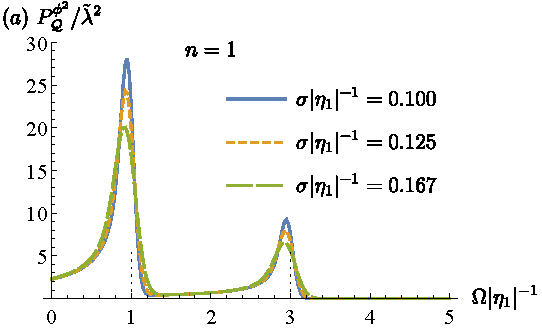
\includegraphics[width=0.45\textwidth]{figures/Fig6a.pdf}
    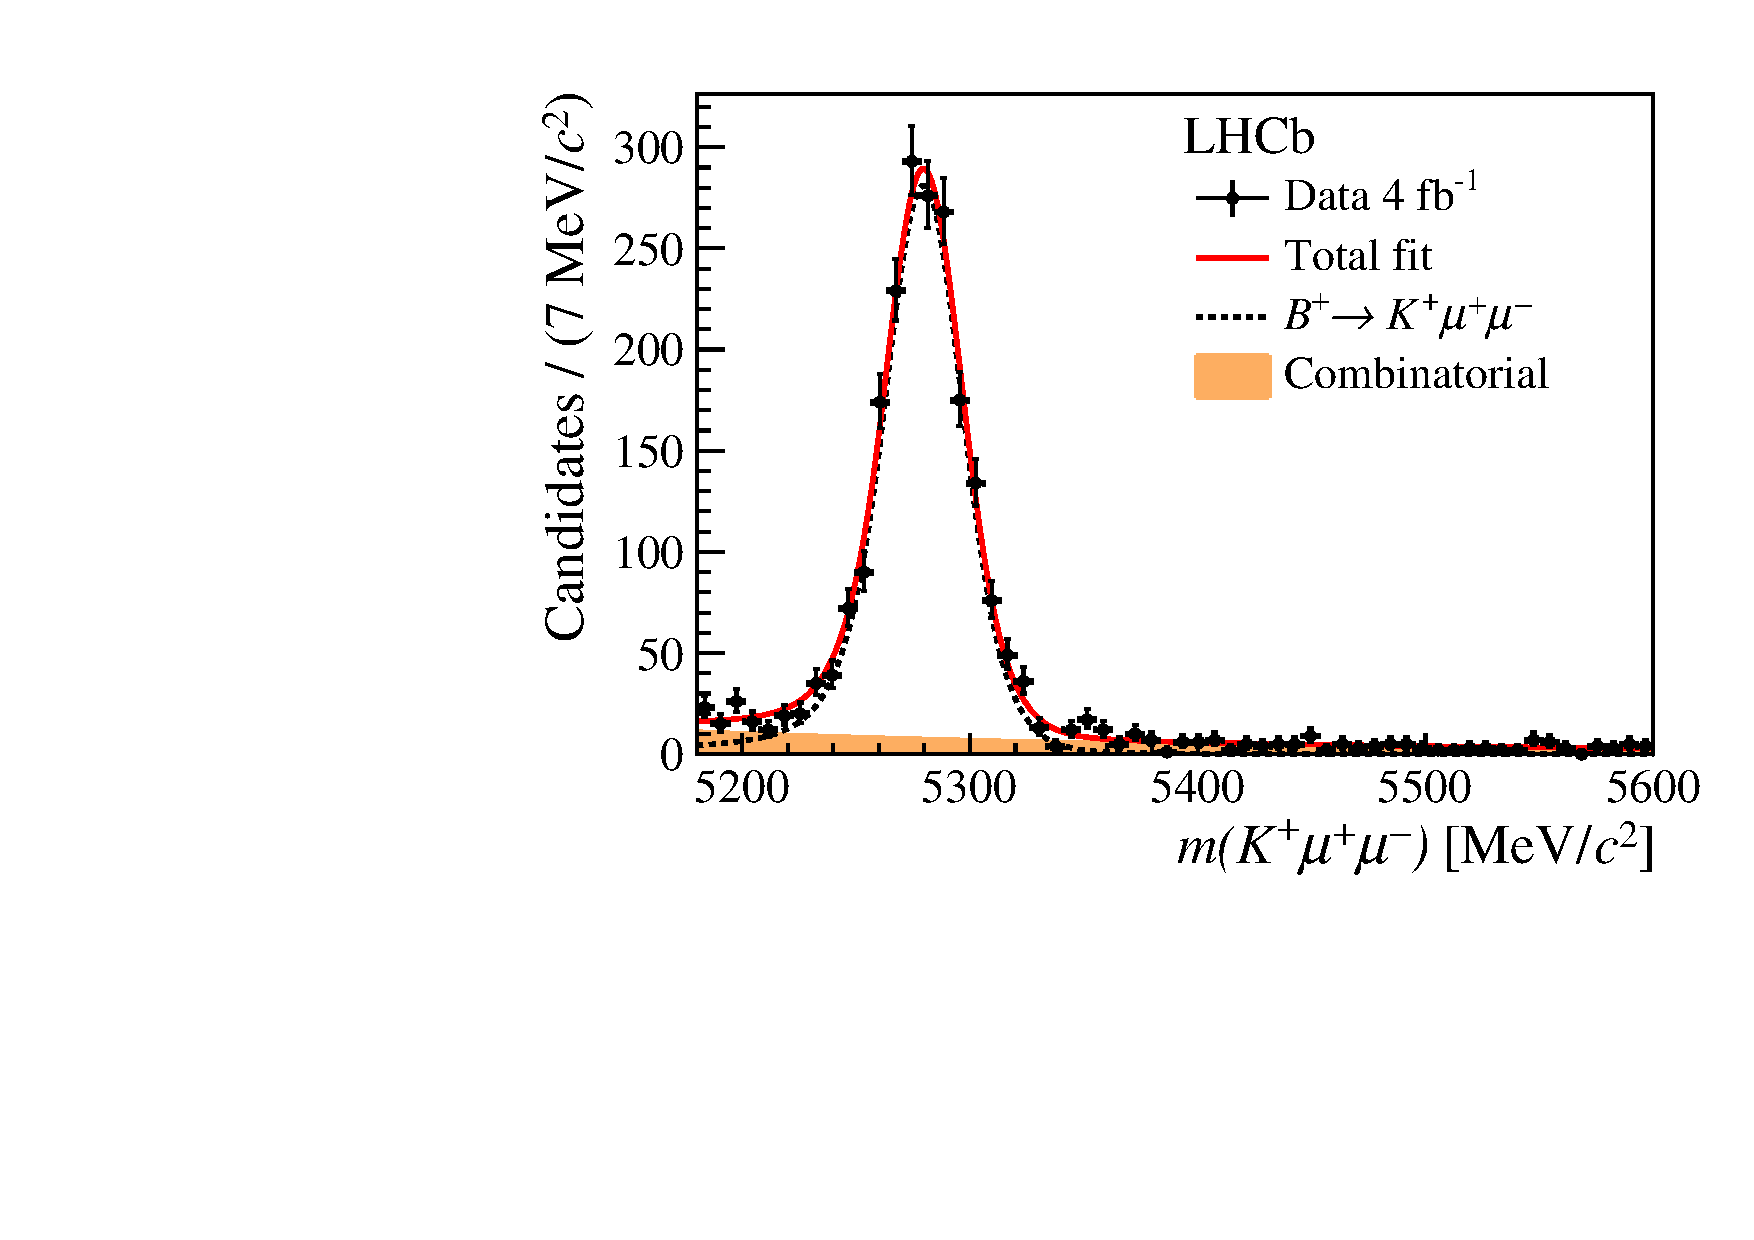
\includegraphics[width=0.45\textwidth]{figures/Fig6b.pdf}

    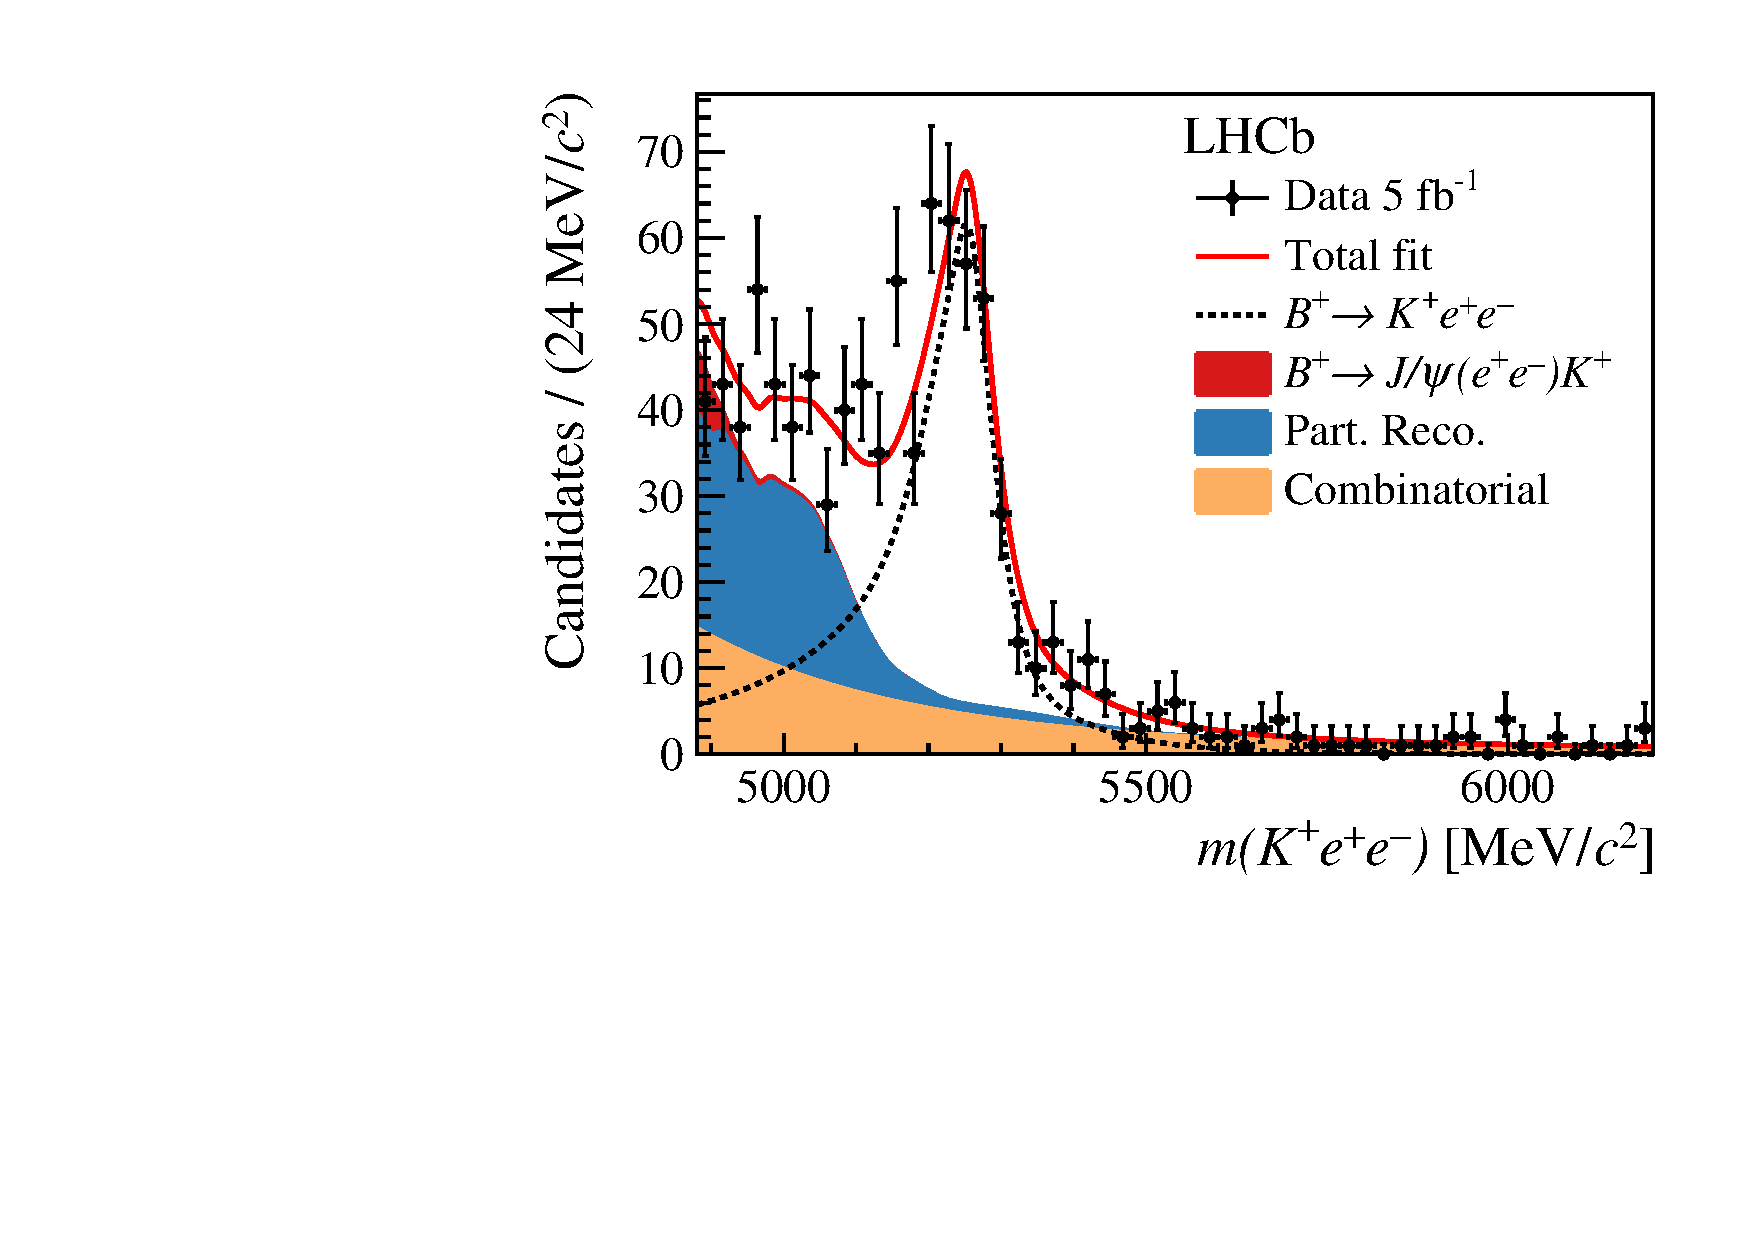
\includegraphics[width=0.45\textwidth]{figures/Fig6c.pdf}
    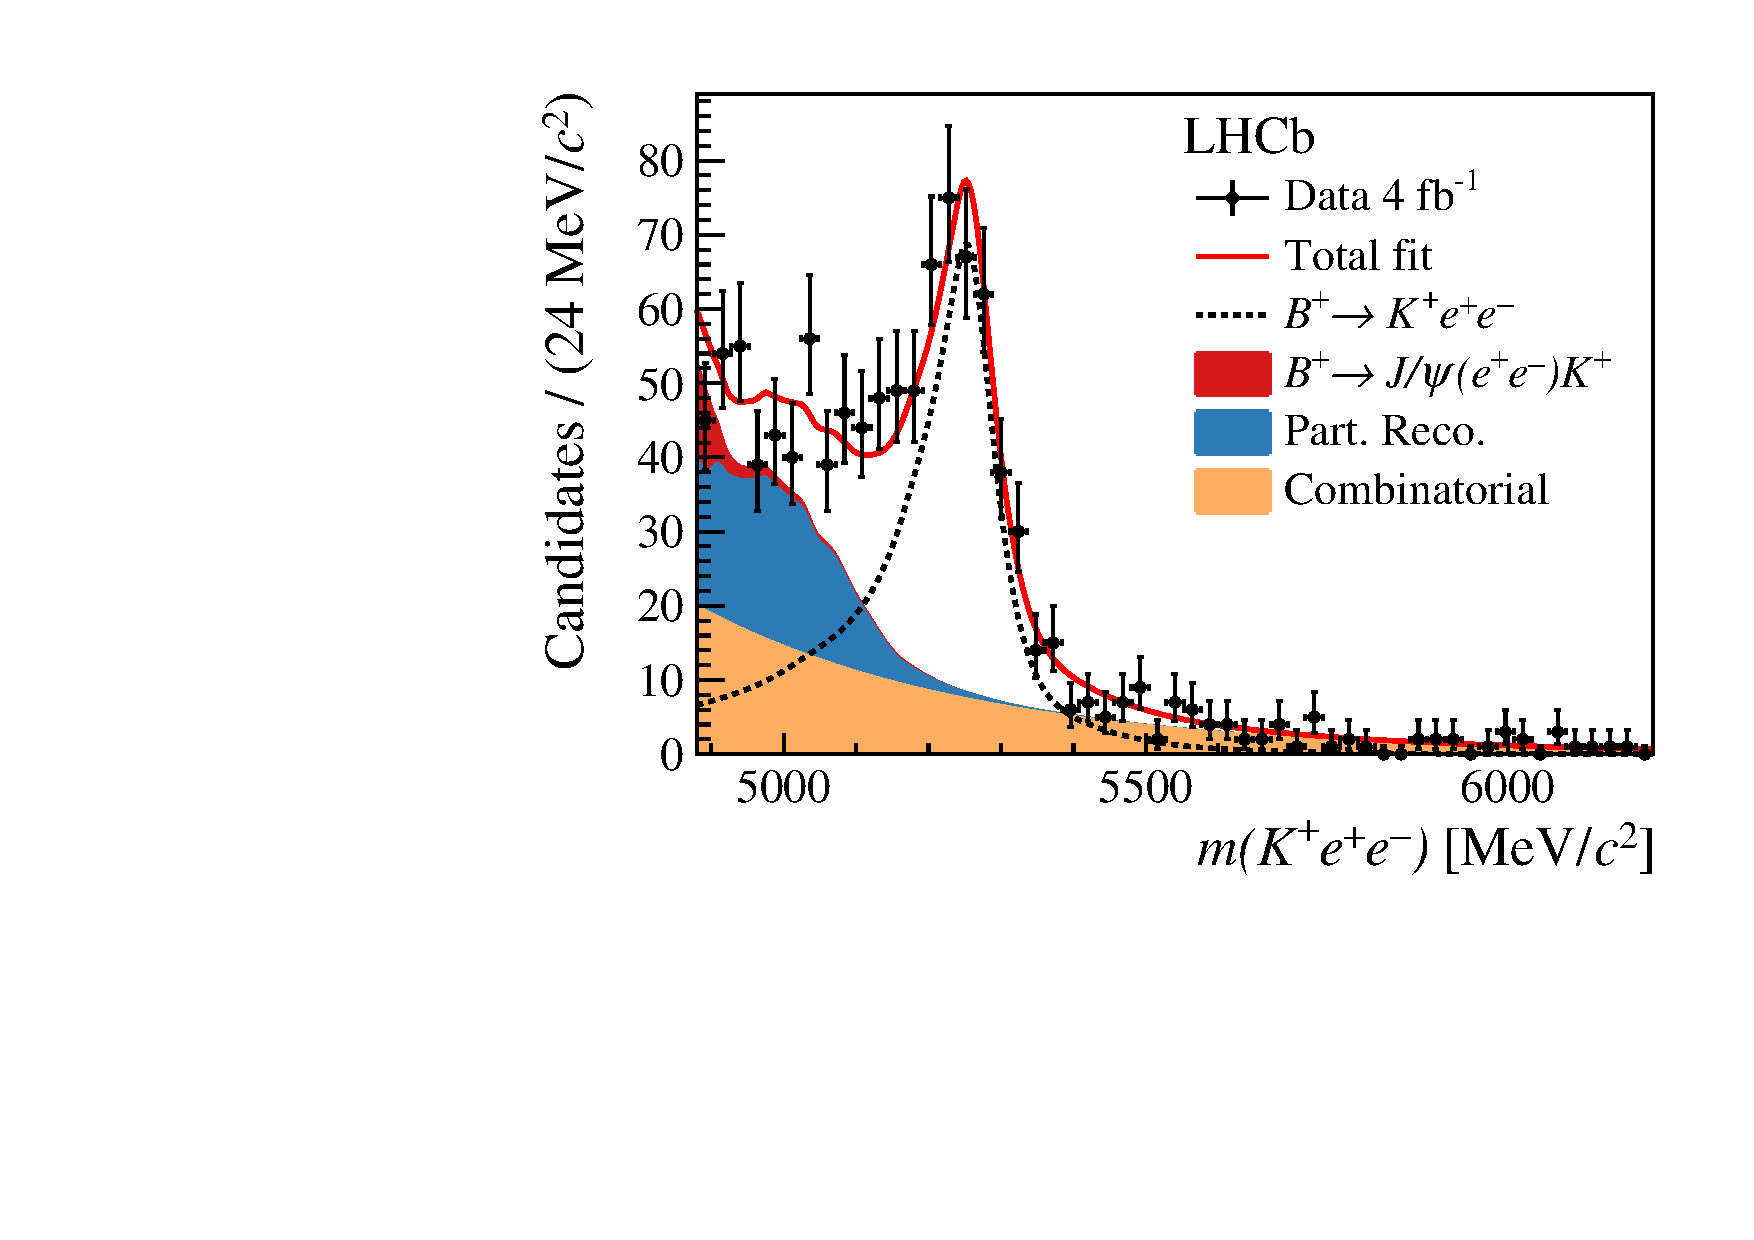
\includegraphics[width=0.45\textwidth]{figures/Fig6d.pdf}
    
    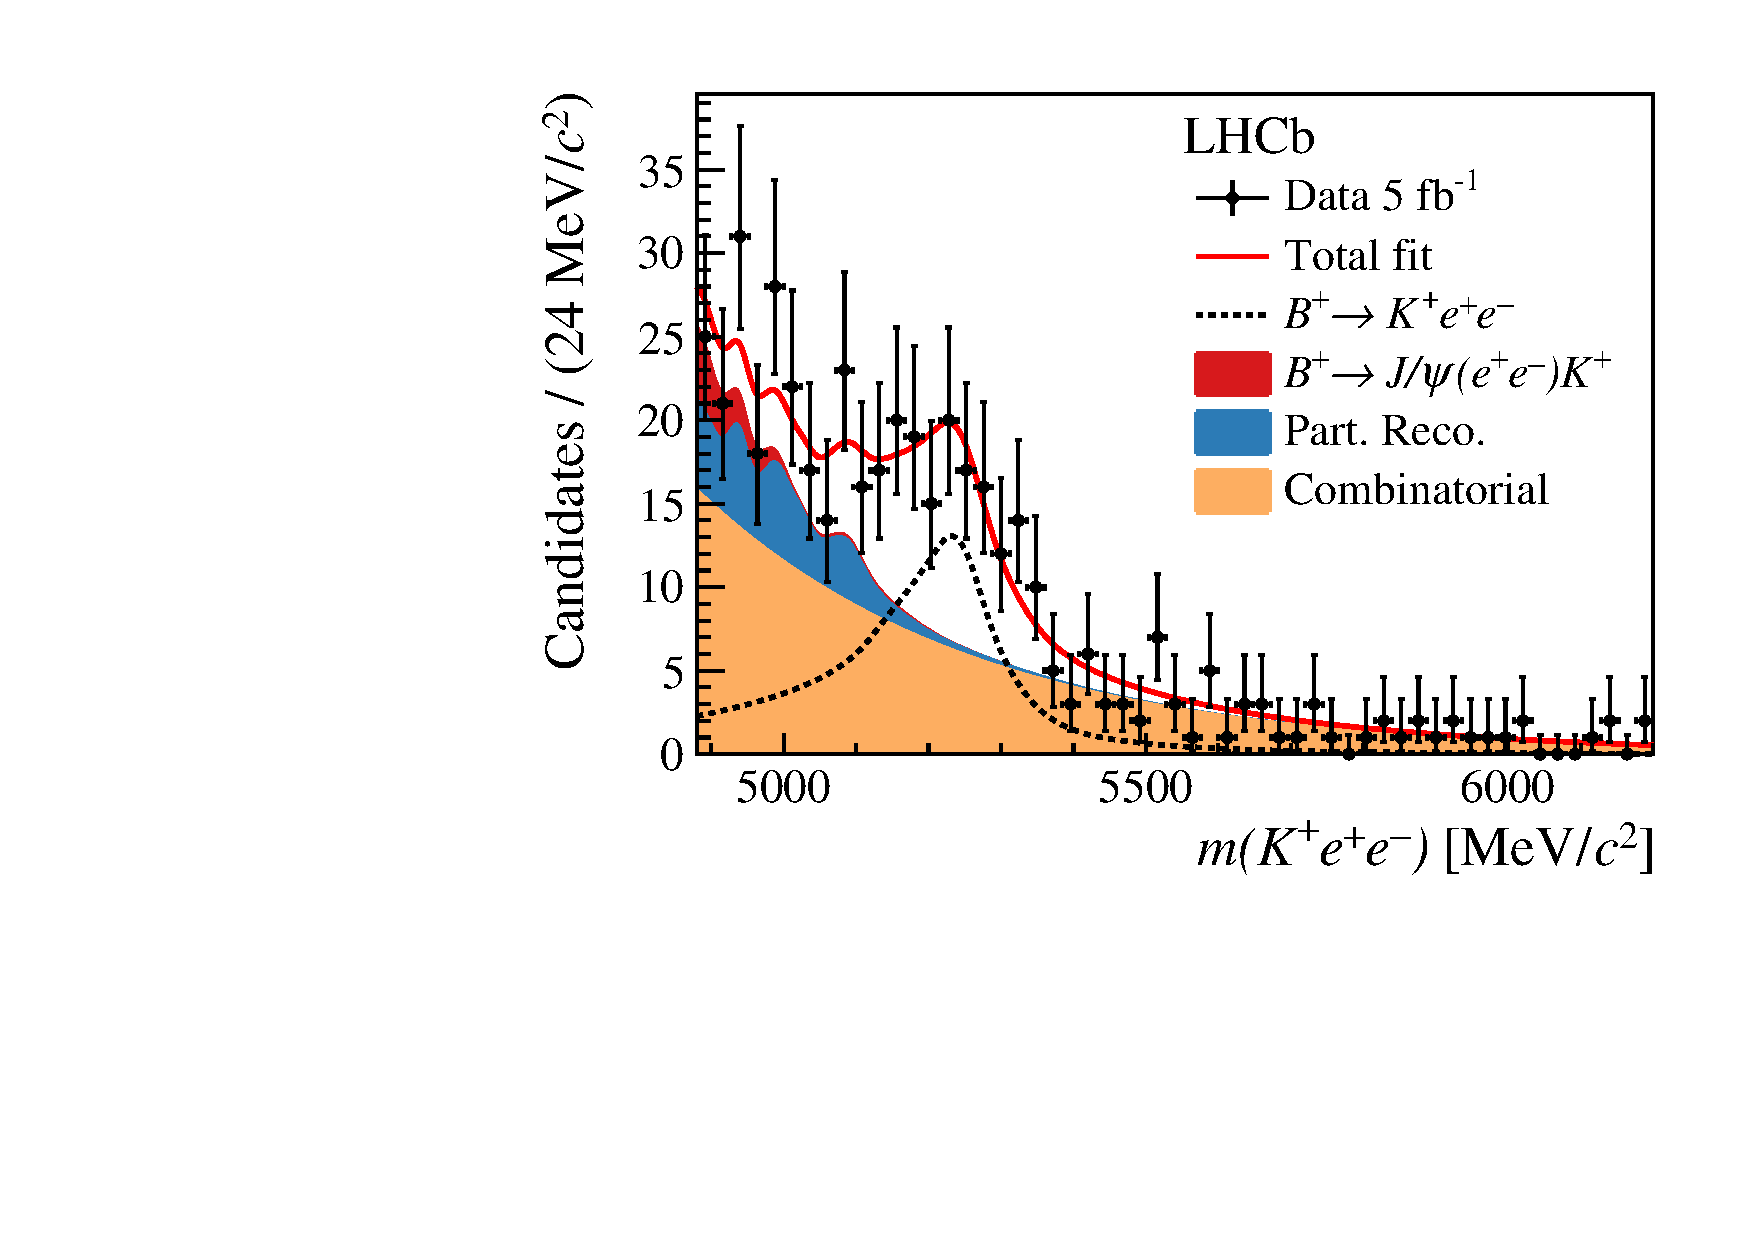
\includegraphics[width=0.45\textwidth]{figures/Fig6e.pdf}
    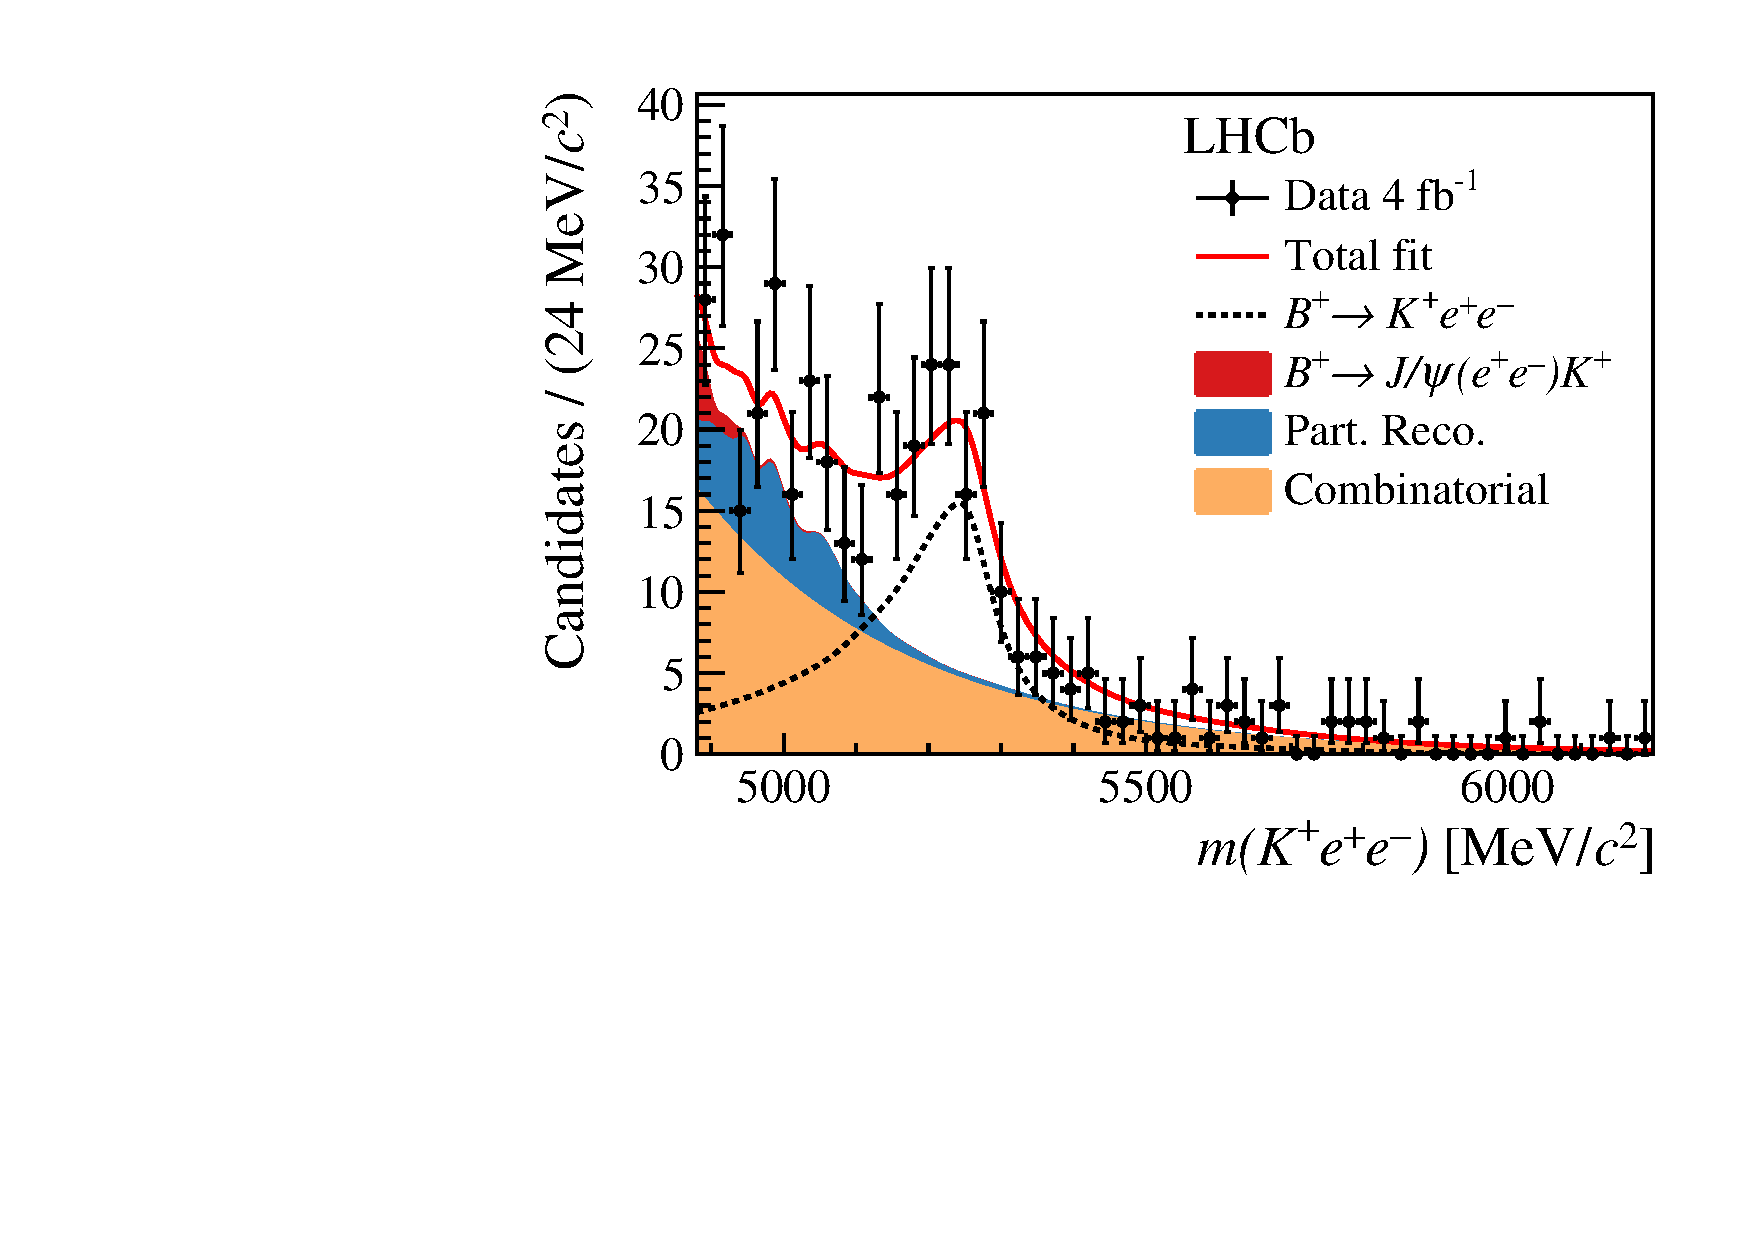
\includegraphics[width=0.45\textwidth]{figures/Fig6f.pdf}
    
    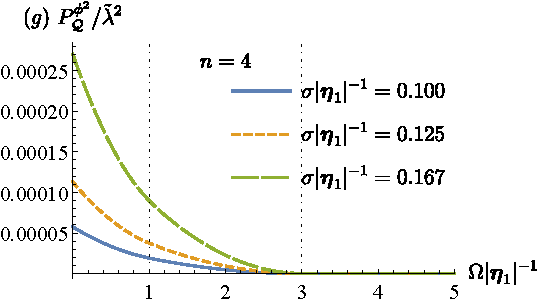
\includegraphics[width=0.45\textwidth]{figures/Fig6g.pdf}
    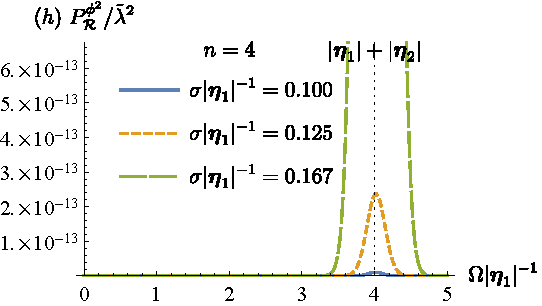
\includegraphics[width=0.45\textwidth]{figures/Fig6h.pdf}
    \caption{Candidate invariant mass distributions. Distribution of the invariant mass \mKll for nonresonant candidates in the (left) sample previously analysed~\cite{LHCb-PAPER-2019-009} and (right) the new data sample. The top row shows the fit to the muon modes and the subsequent rows the fits to the electron modes triggered by (second row) one of the electrons, (third row) the kaon and (last row) by other particles in the event. The fit projections are superimposed.
    }
    \label{fig:nonresfits_categories}
\end{figure}


\begin{figure}
    \centering
    % \includegraphics[width=0.45\textwidth]{figures/FigS5a.pdf}
    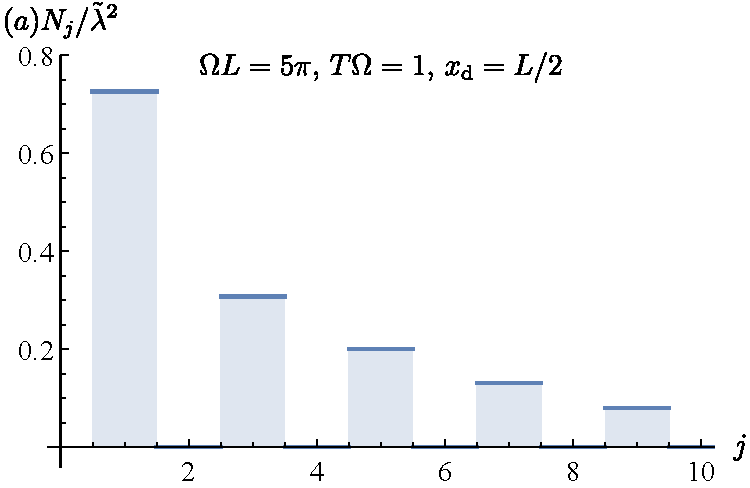
\includegraphics[width=0.45\textwidth]{figures/Fig7a.pdf}
    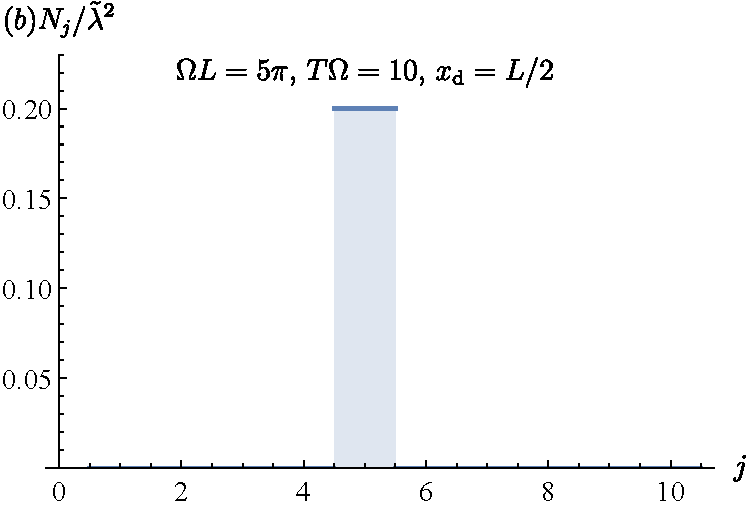
\includegraphics[width=0.45\textwidth]{figures/Fig7b.pdf}
    
    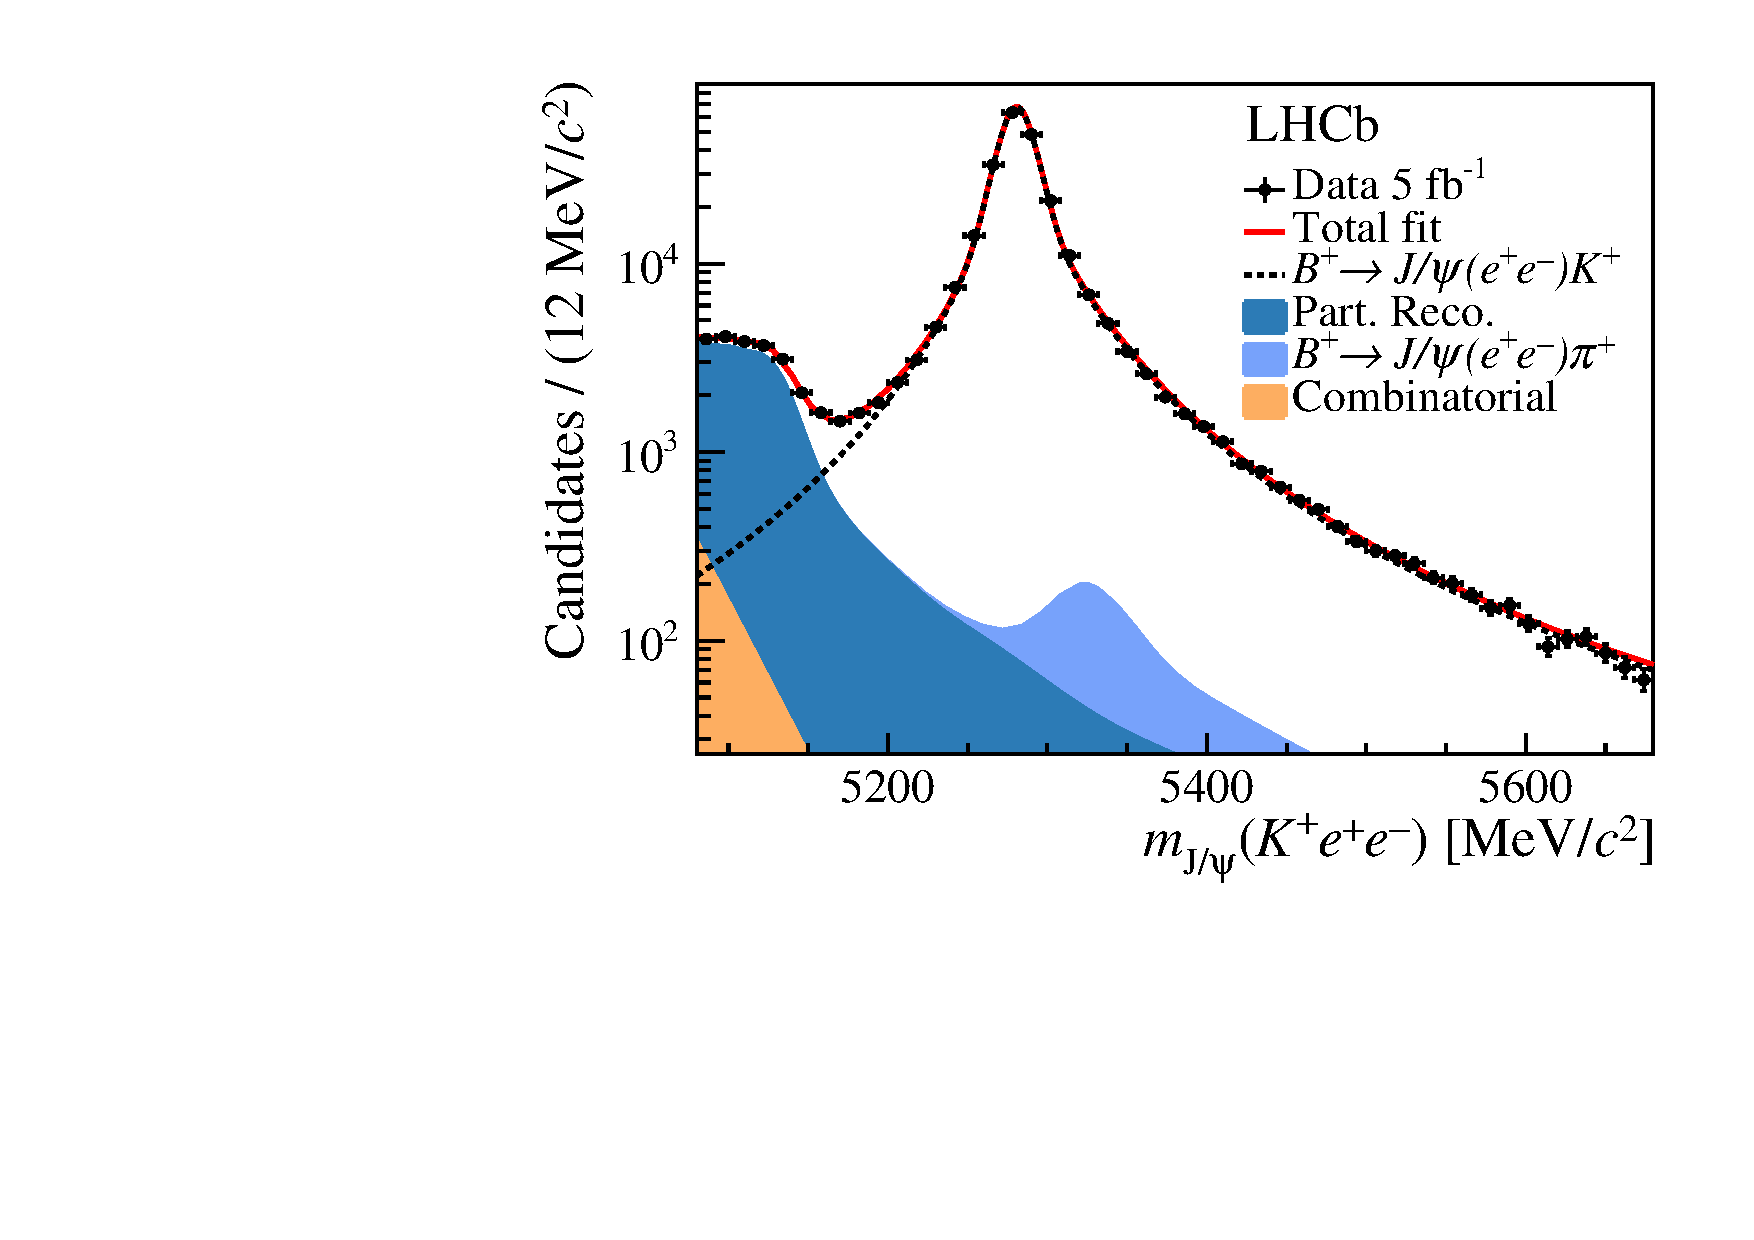
\includegraphics[width=0.45\textwidth]{figures/Fig7c.pdf}
    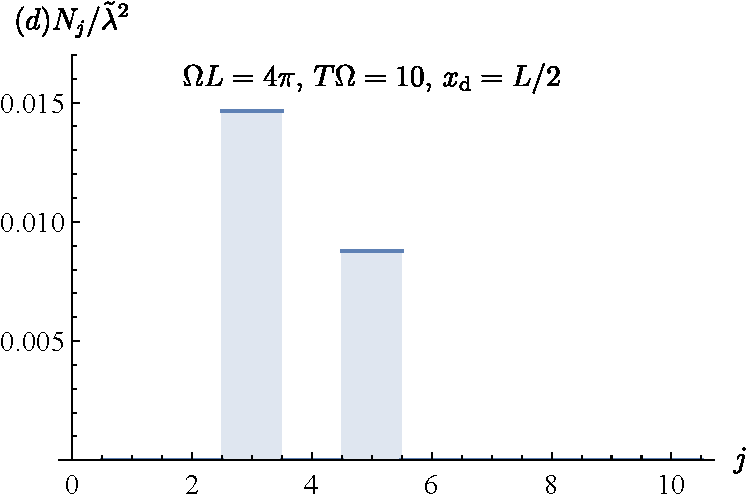
\includegraphics[width=0.45\textwidth]{figures/Fig7d.pdf}
    
    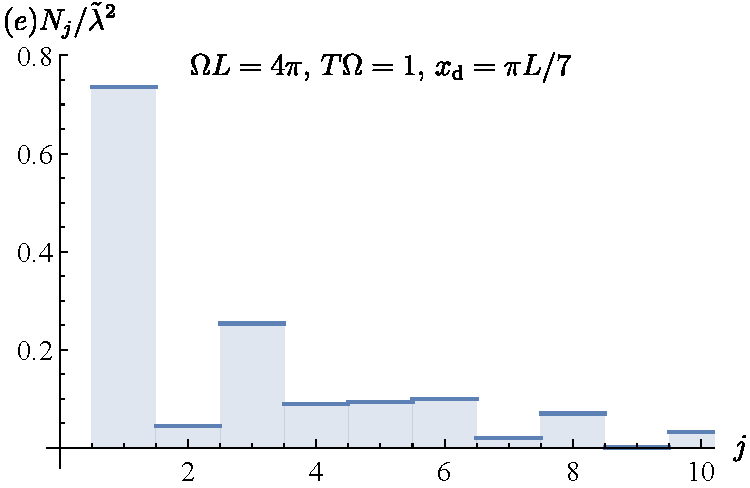
\includegraphics[width=0.45\textwidth]{figures/Fig7e.pdf}
    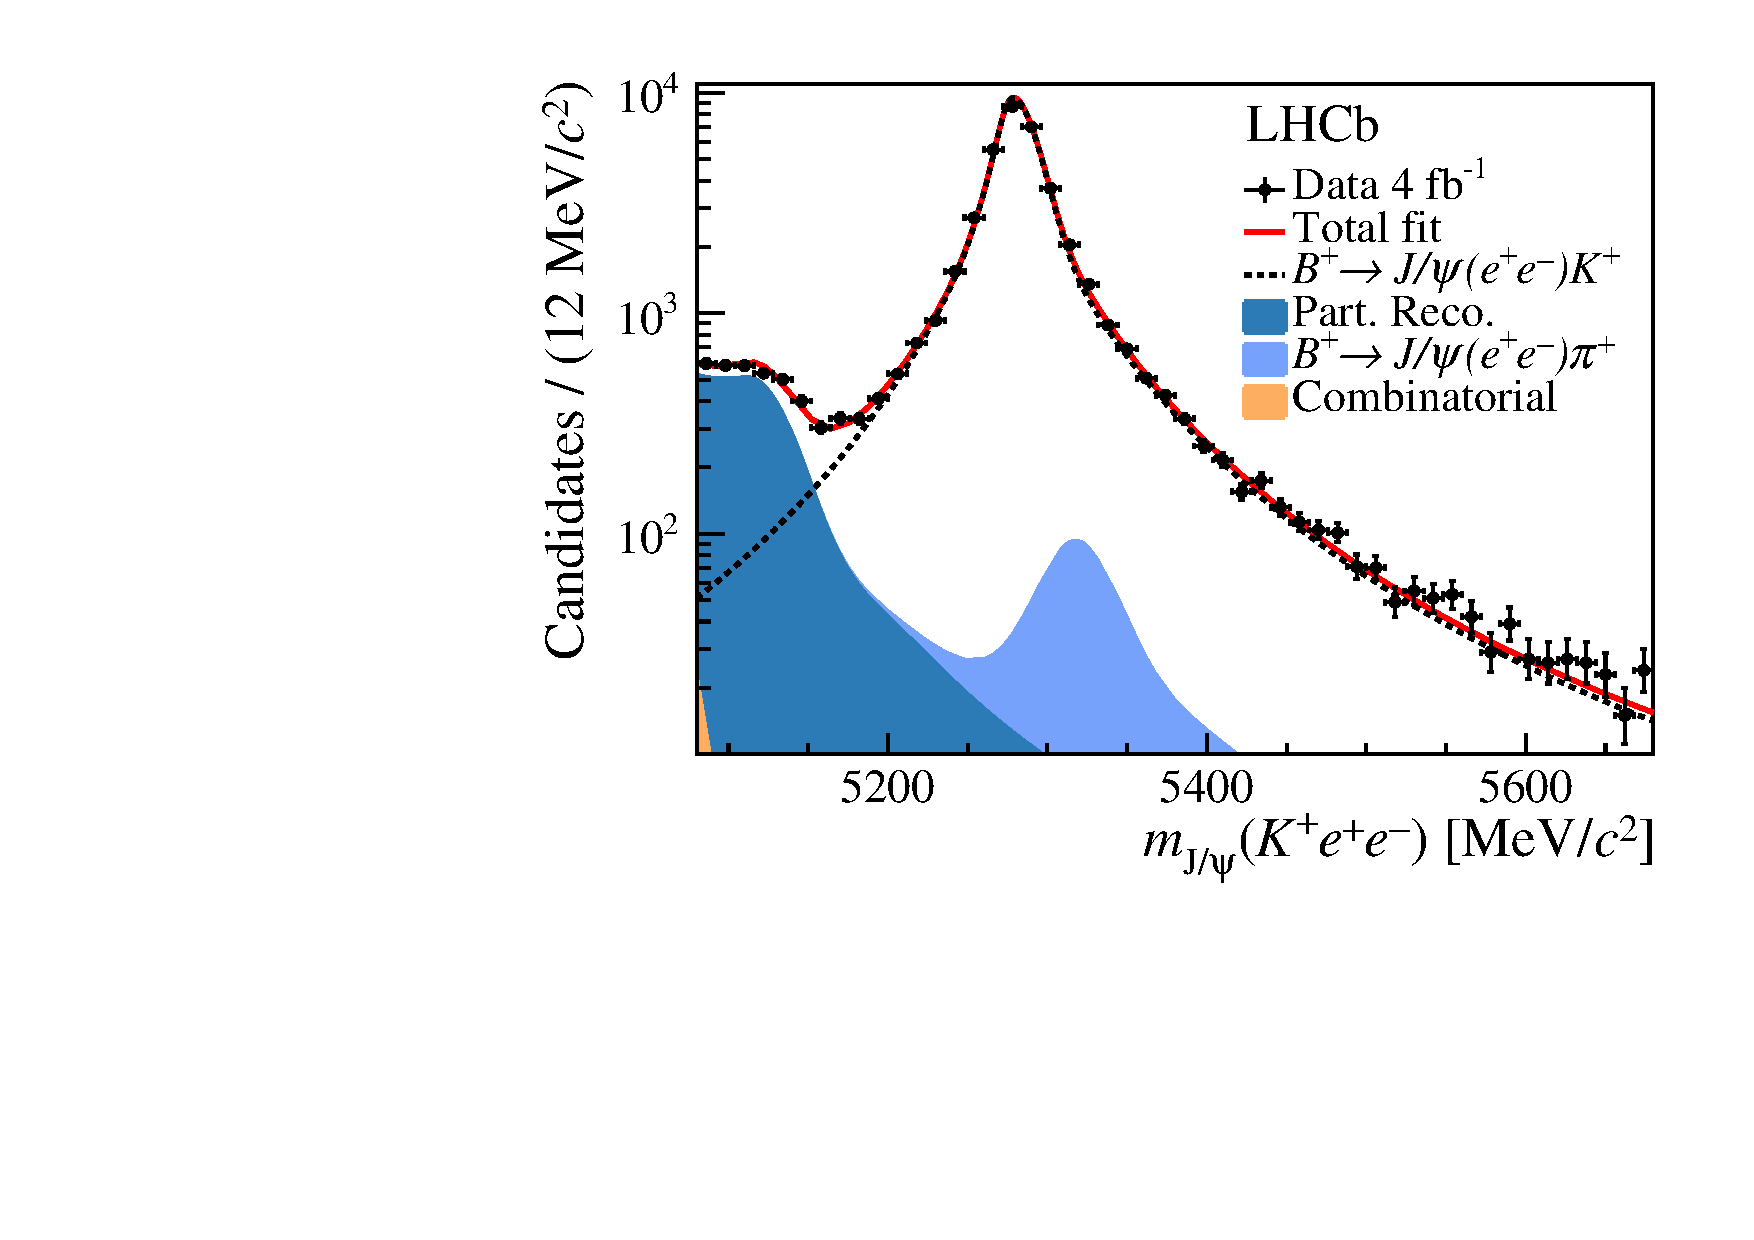
\includegraphics[width=0.45\textwidth]{figures/Fig7f.pdf}
    
    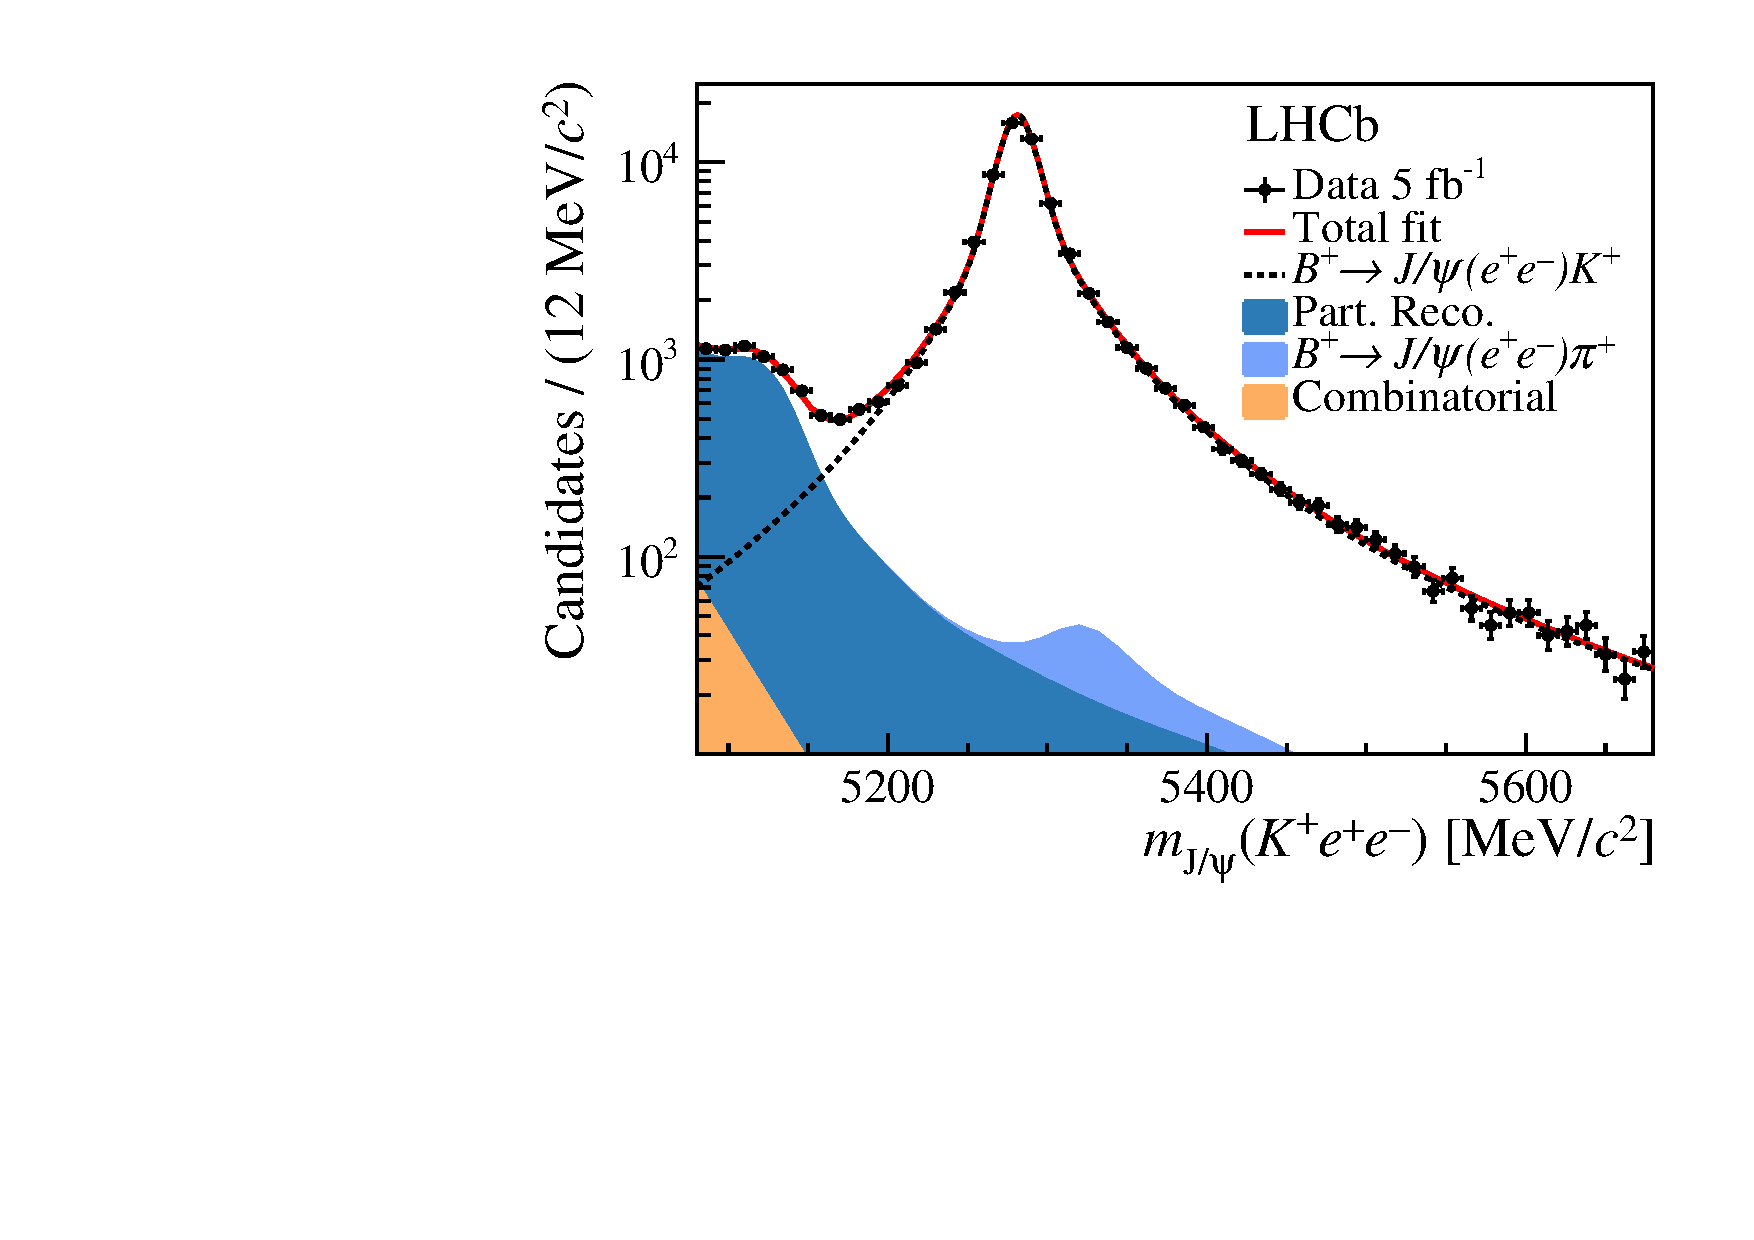
\includegraphics[width=0.45\textwidth]{figures/Fig7g.pdf}
    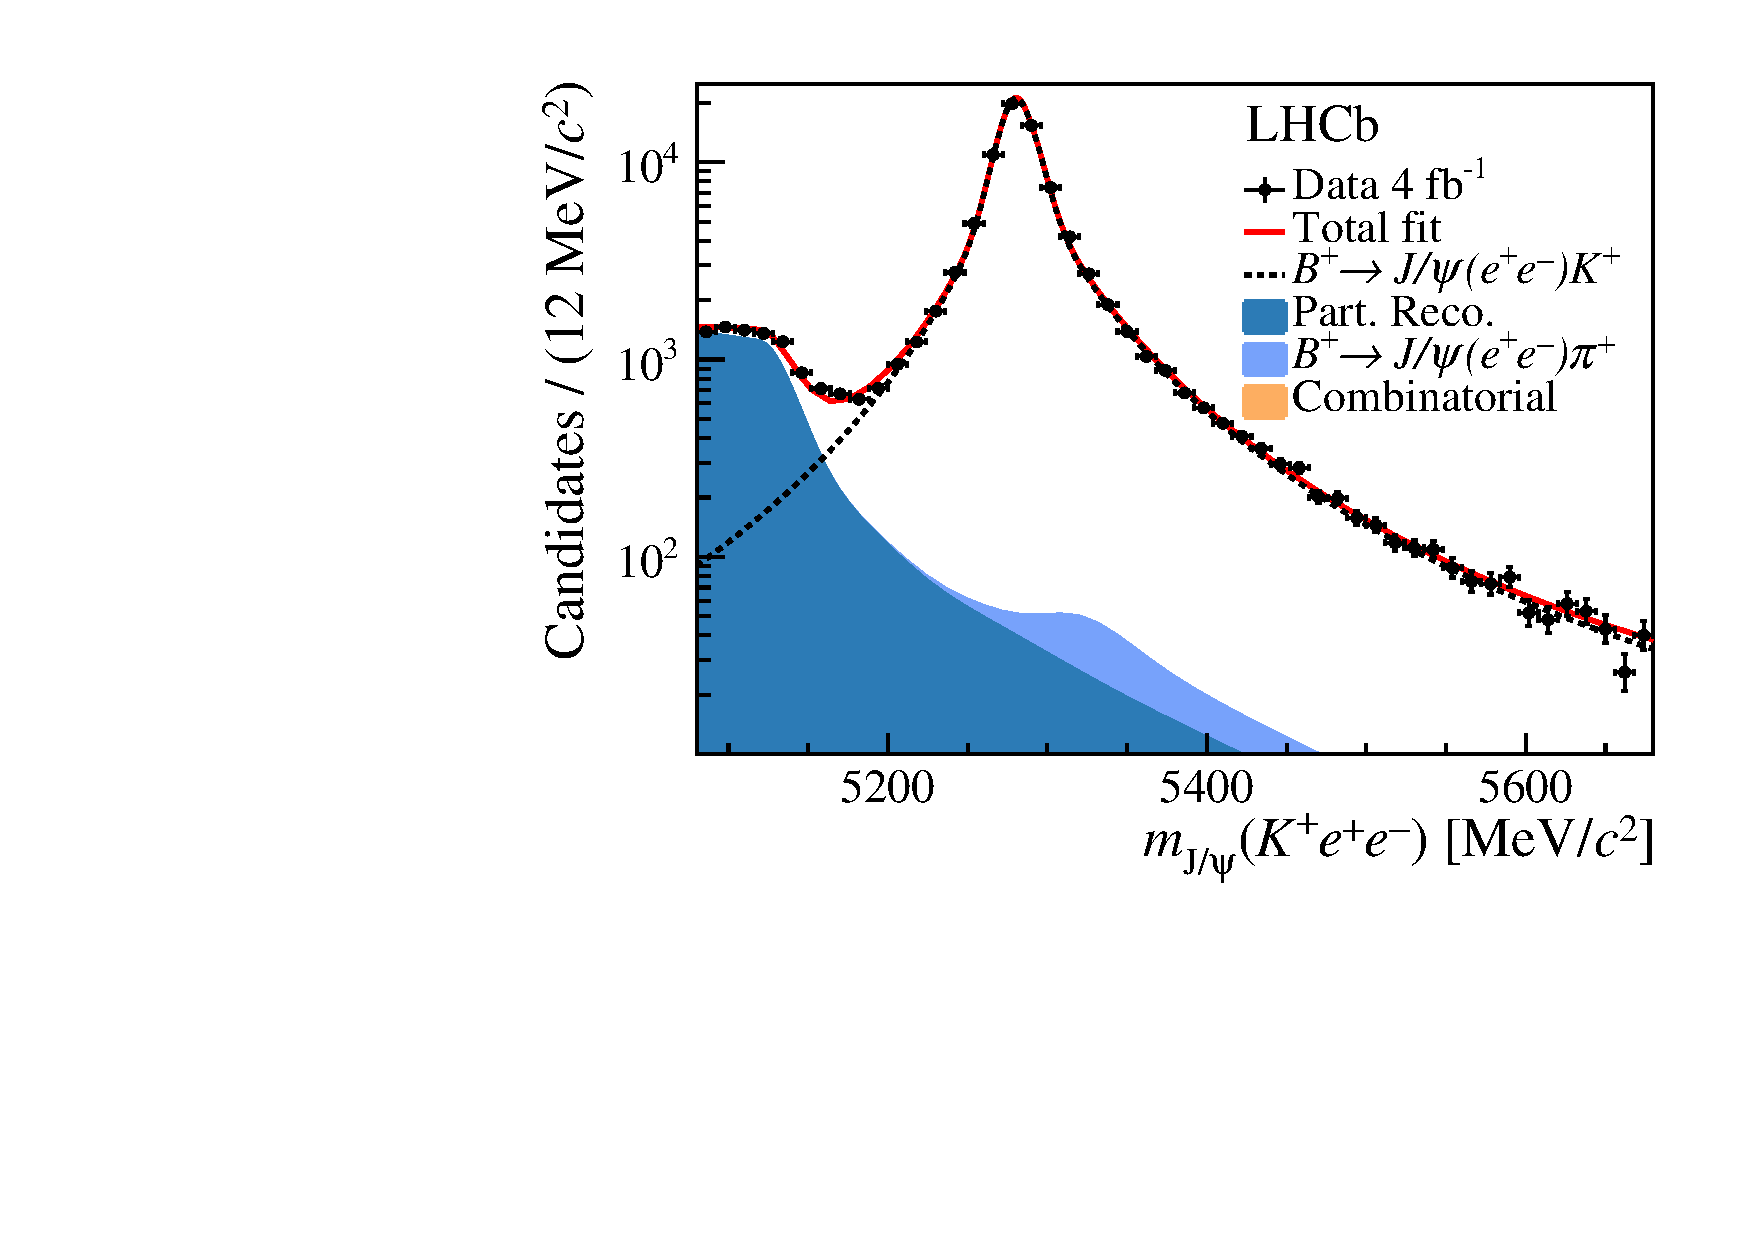
\includegraphics[width=0.45\textwidth]{figures/Fig7h.pdf}
    
    \caption{Candidate invariant mass distributions. Distribution of the invariant mass \mKllconst for resonant candidates in the (left) sample previously analysed~\cite{LHCb-PAPER-2019-009} and (right) the new data sample. The top row shows the fit to the muon modes and the subsequent rows the fits to the electron modes triggered by (second row) one of the electrons, (third row) the kaon and (last row) by other particles in the event. The fit projections are superimposed.
}
    \label{fig:resfits_categories}
\end{figure}


The profile likelihood for the fit to the nonresonant decays is shown in Fig.~\ref{fig:profile_likelihood}. The likelihood is non-Gaussian in the region $\RK>0.95$ due to the comparatively low yield of \BuKee events. 
Following the procedure described in Refs.~\cite{LHCb-PAPER-2019-009, LHCb-PAPER-2017-013}, the p-value is computed by integrating the posterior probability density function for \RK, having folded in the theory uncertainty on the SM prediction, for \RK values larger than the SM  expectation. The corresponding significance in terms of standard deviations is computed using the inverse Gaussian cumulative distribution function for a one-sided conversion.

A test statistic is constructed that is based on the likelihood ratio between two hypotheses with common (null) or different (test) \RK values for the part of the sample analysed previously (7, 8 and part of the 13\tev data) and for the new portion of the 13\tev data. Using pseudoexperiments based on the null hypothesis, the data suggest that the \RK value from the new portion of the data is compatible with that from the previous sample with a p-value of 95\%. Further tests give good compatibility for subsamples of the data corresponding to different trigger categories and magnet polarities.

The departure of the profile likelihood shown in Fig.~\ref{fig:profile_likelihood} from a normal distribution stems from the  definition of \RK. In particular,
in the \RK ratio the denominator is affected by larger statistical uncertainties than the numerator, owing to the larger number of nonresonant muonic signal candidates. However, the intervals of the likelihood distribution are found to be the same when estimated with $1/\RK$ as the fit parameter.


\begin{figure}[!t]
   \begin{center}
      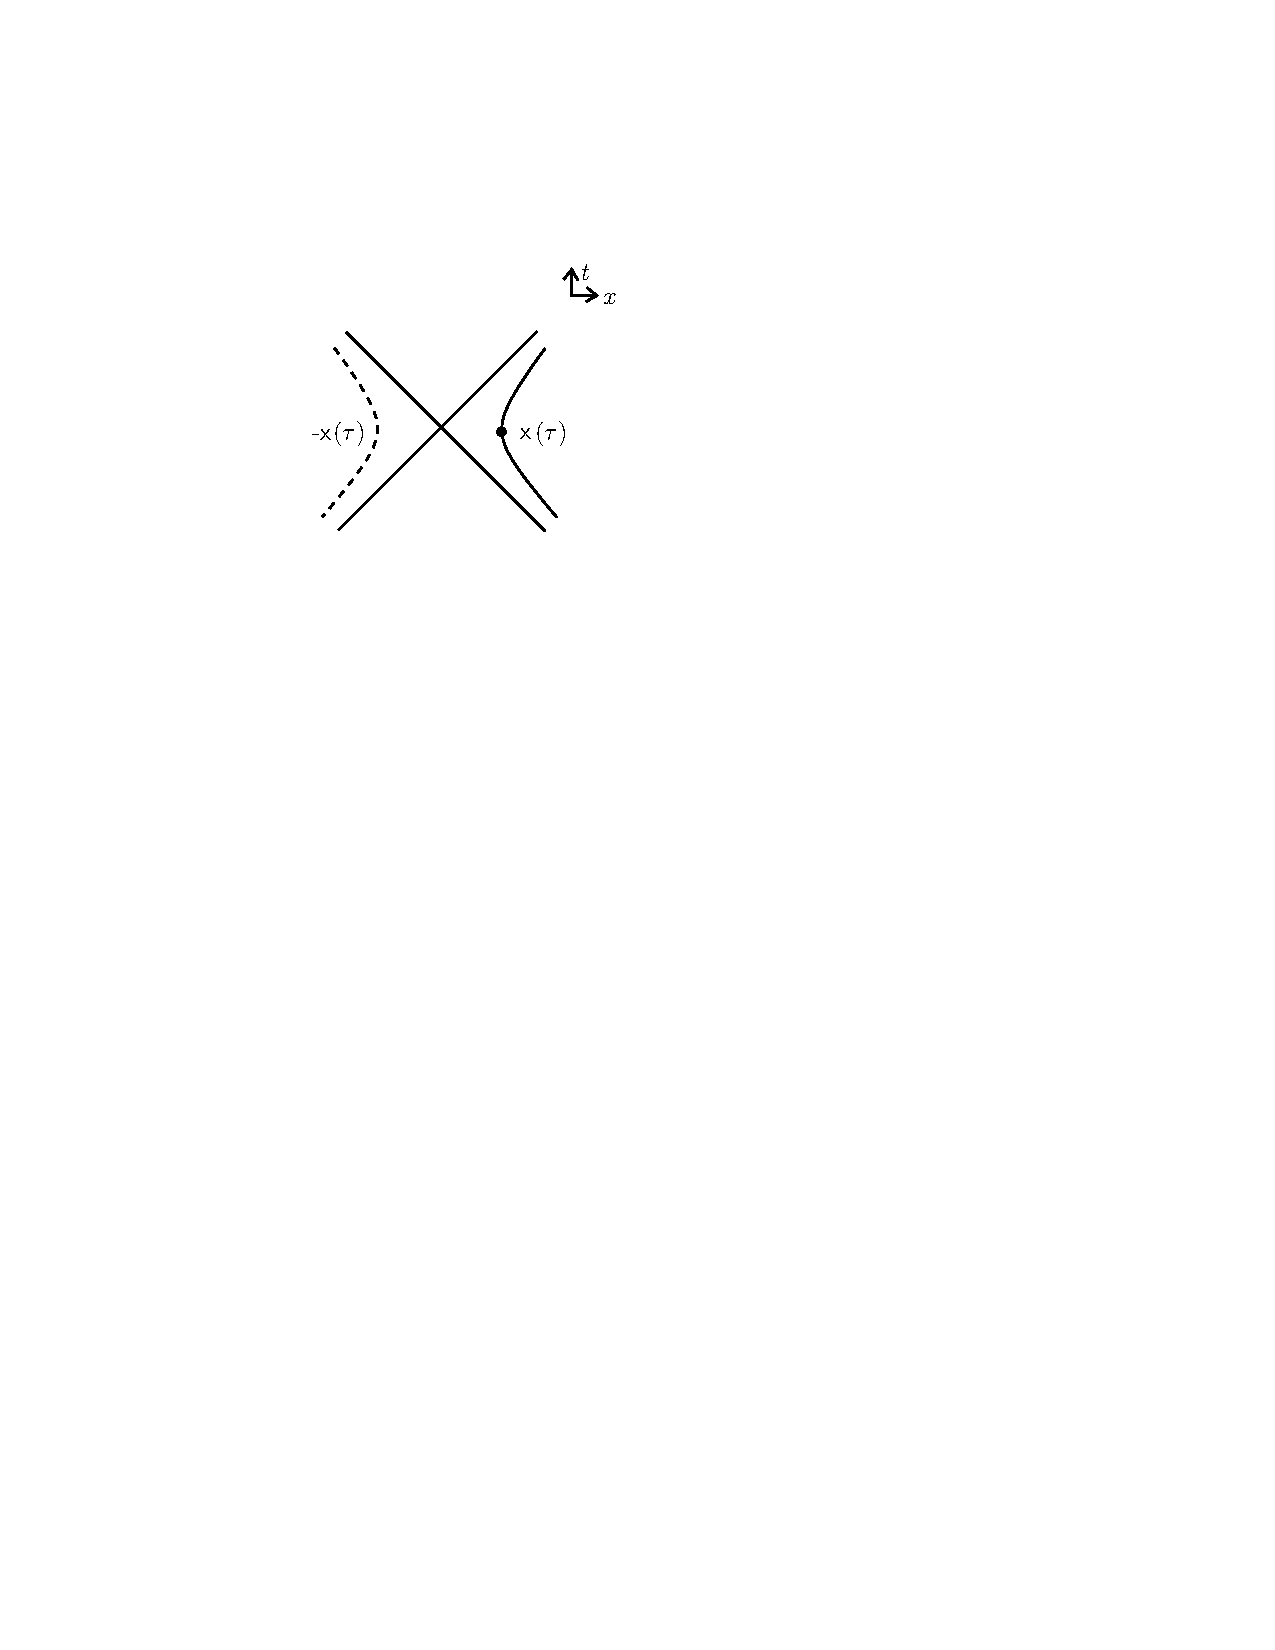
\includegraphics[height=0.25\textheight]{figures/Fig8.pdf}
  \end{center}
     \caption{Likelihood function from the fit to the nonresonant \BuKll candidates profiled as a function of \RK. The extent of the  dark, medium and light blue  regions shows the values allowed for \RK at $1\sigma$, $3\sigma$ and $5\sigma$ levels. The red line indicates the prediction from the SM. }
    \label{fig:profile_likelihood}
\end{figure}



\subsubsection*{Additional cross-checks} 

The \rjpsi single ratio is used to perform a number of additional cross-checks. The distribution of this ratio as a function of the angle between the leptons and the minimum \pt of the leptons is shown in Fig.~\ref{fig:rjpsi_differential1}, together with the spectra expected for the resonant and nonresonant decays.
No significant trend is observed in either \rjpsi distribution. Assuming the deviations observed are genuine mismodelling of the efficiencies, rather than statistical fluctuations, a total shift of \RK at a level less than $0.001$ would be expected due to these effects. This estimate takes into account the spectrum of the relevant variables in the nonresonant decay modes of interest and is compatible with the estimated systematic uncertainties on \RK. Similarly, the variations seen in \rjpsi as a function of all other reconstructed quantities examined are compatible with the systematic uncertainties assigned. In addition, \rjpsi is computed in two-dimensional intervals of reconstructed quantities, as shown in Fig.~\ref{fig:rjpsi_bin}. Again, no significant trend is seen.
 
\begin{figure}[!t]
   \begin{center}
   \begin{overpic}[width=0.45\linewidth,trim={0 0 0 0.5cm}, clip]{figures/Fig9a.pdf}
   \put(50,26){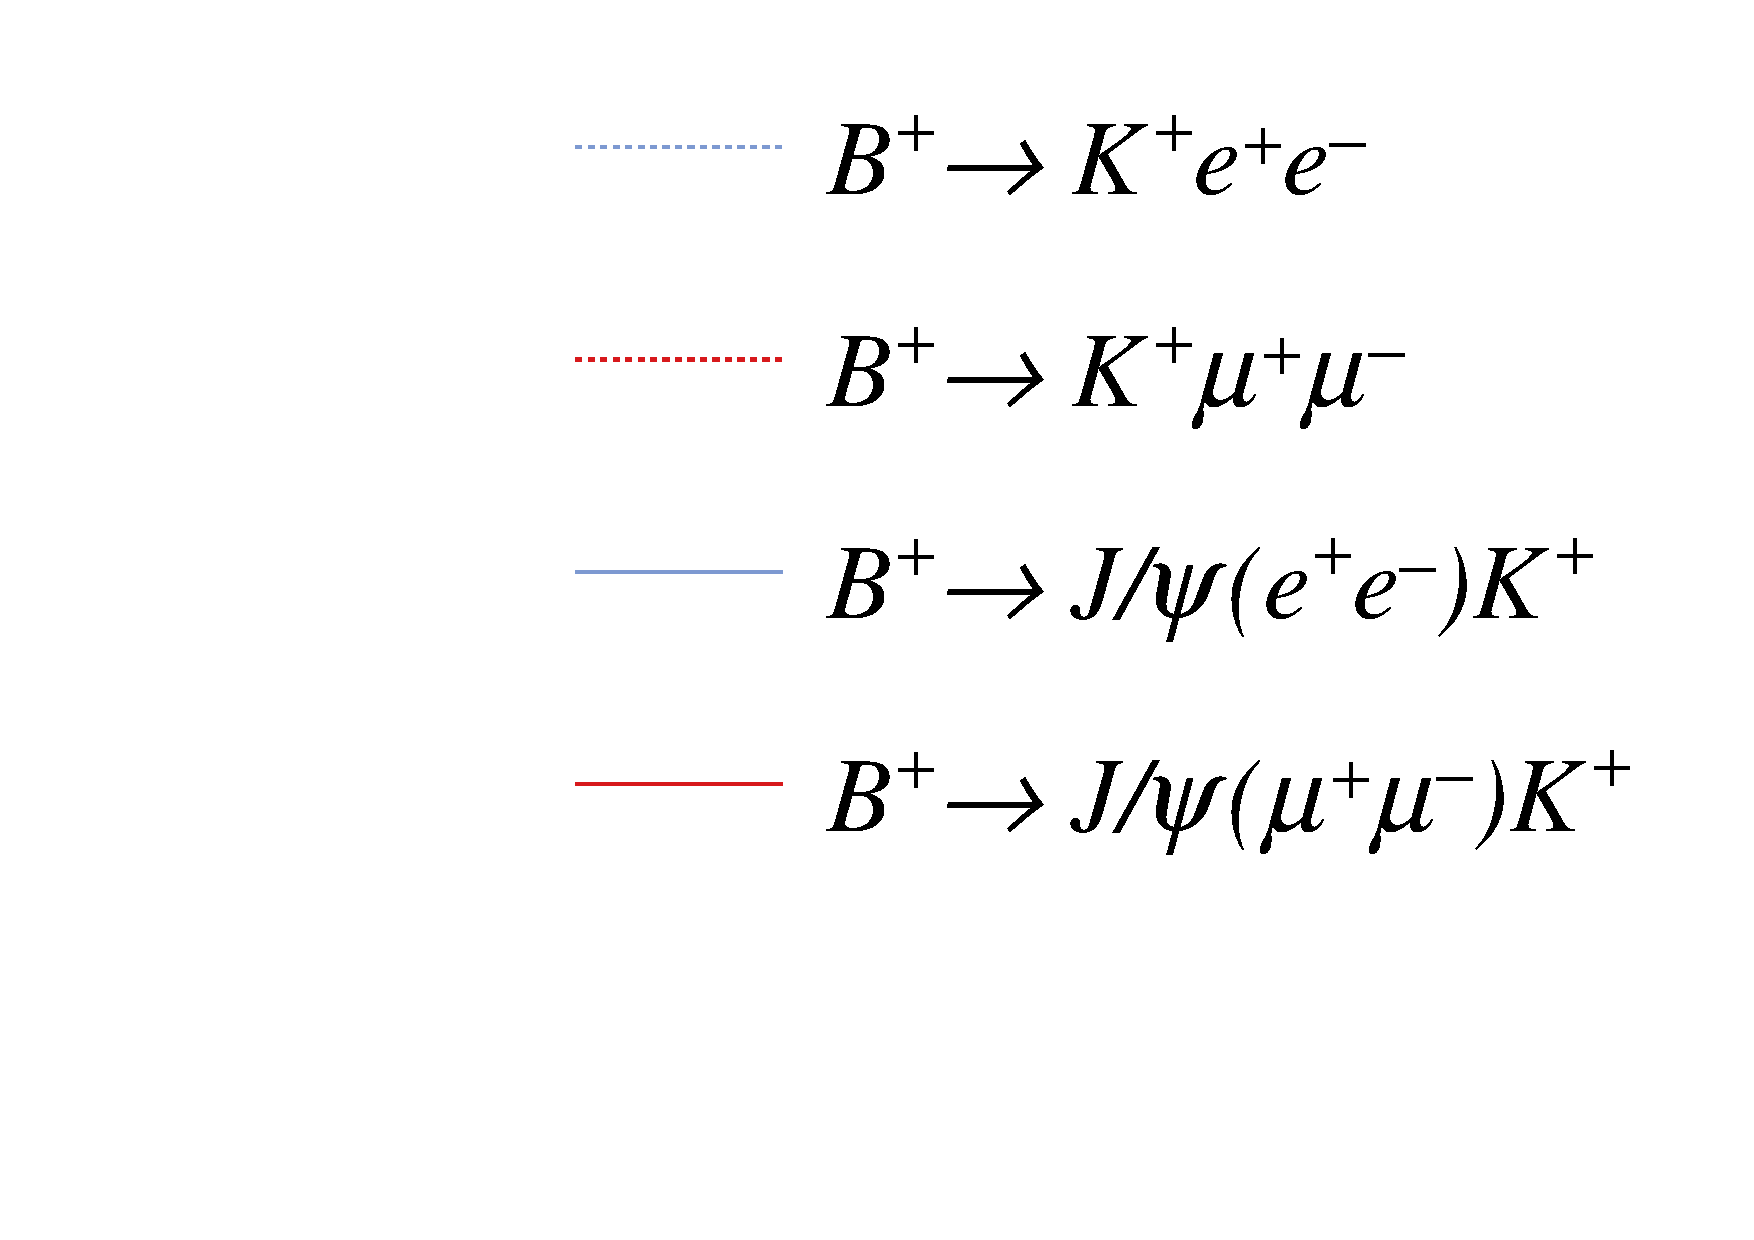
\includegraphics[width=0.2\linewidth]{figures/Fig9e.pdf}}
   \end{overpic}
   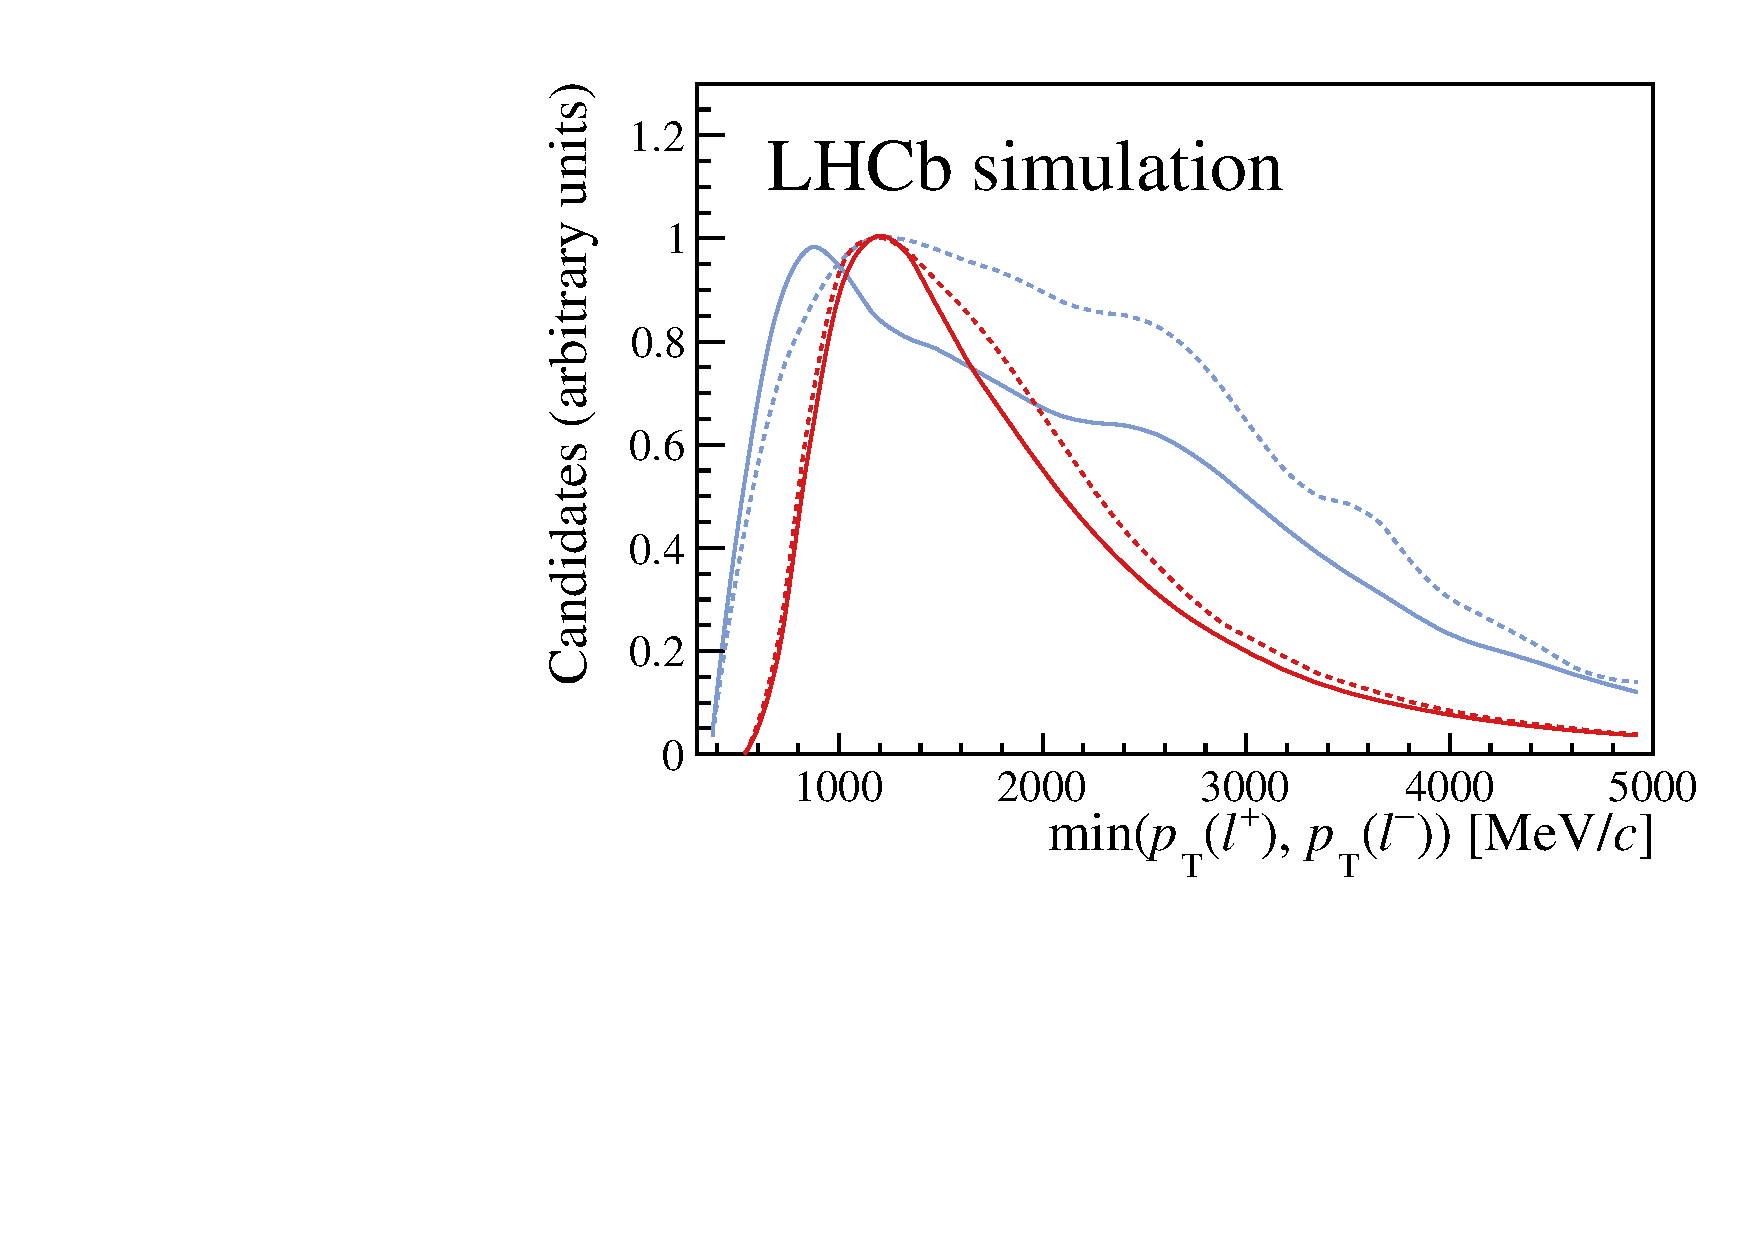
\includegraphics[width=0.45\linewidth,trim={0 0.15cm 0 0}, clip]{figures/Fig9b.pdf}
   
  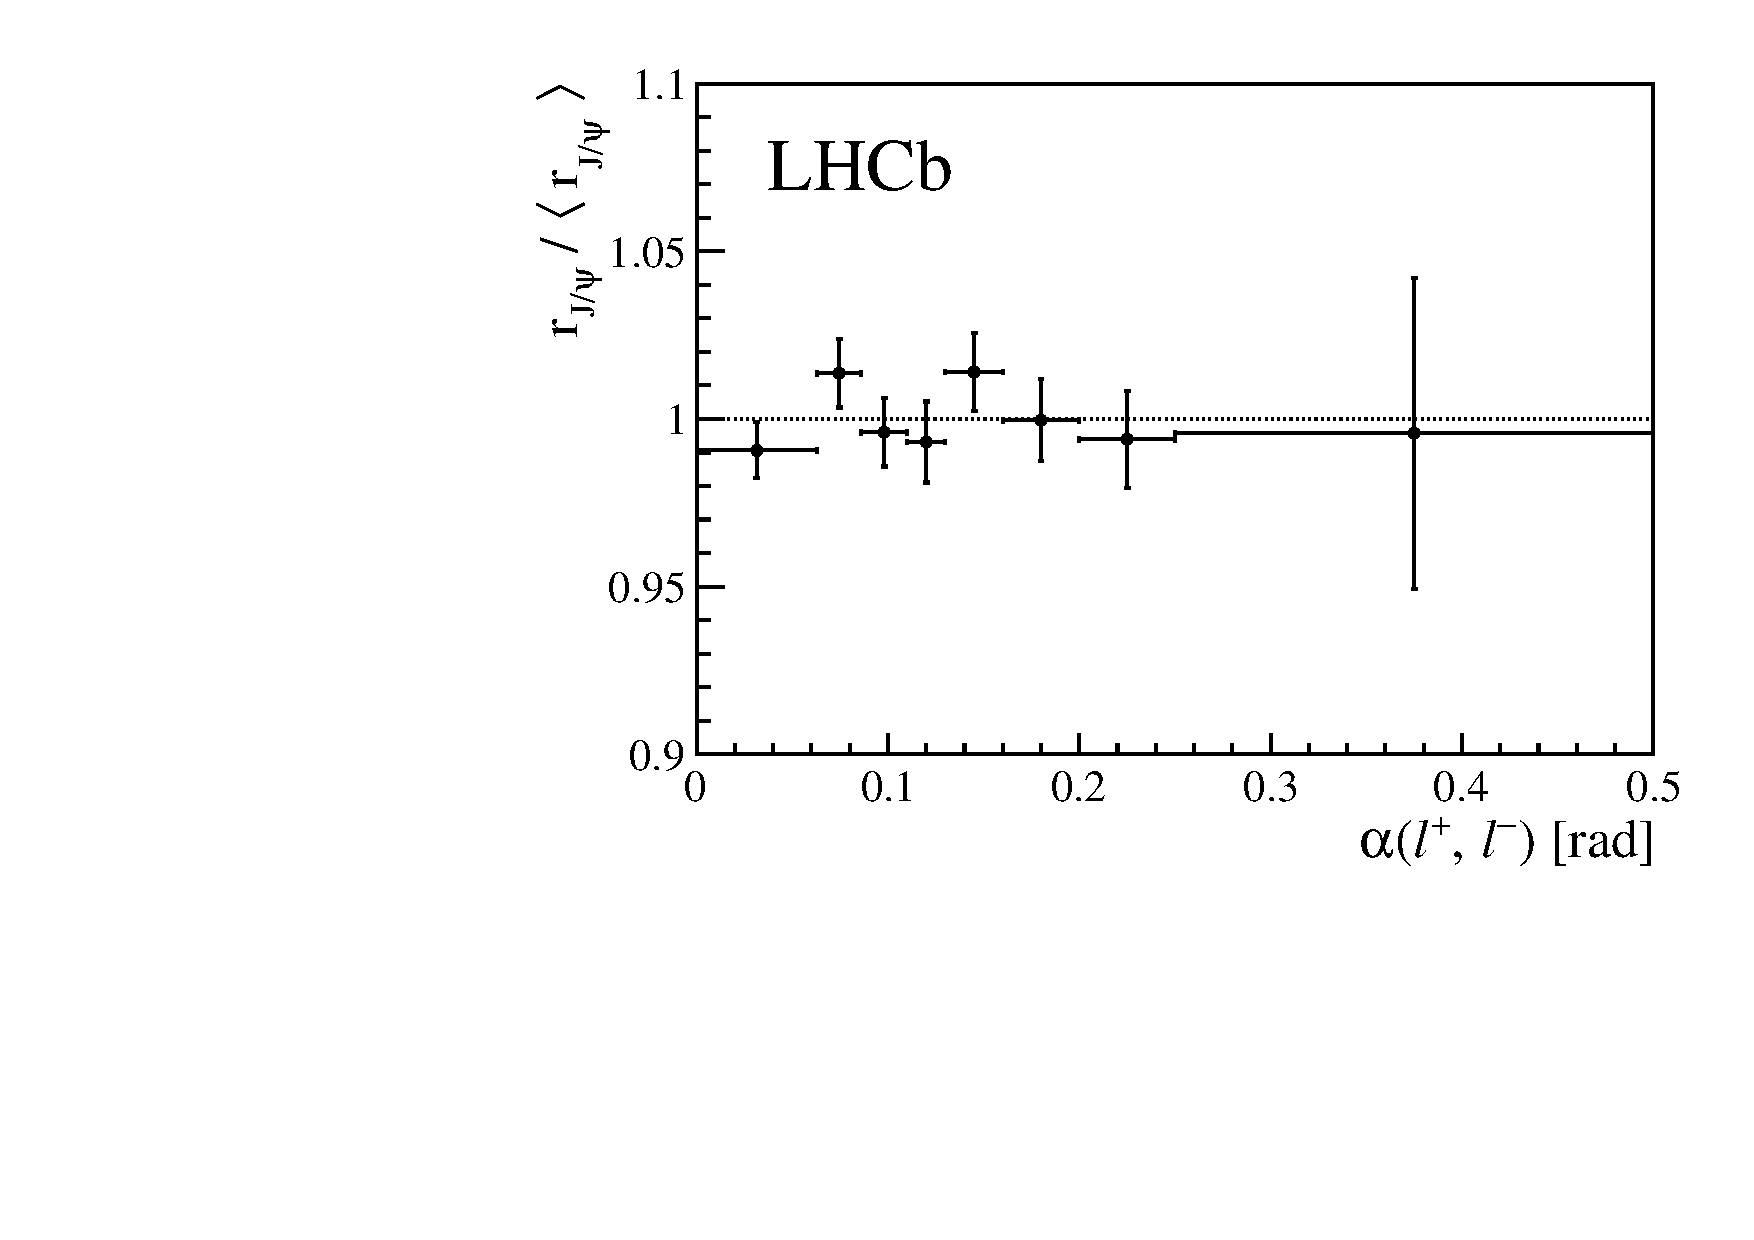
\includegraphics[width=0.45\linewidth,trim={0 0 0 0.5cm}, clip]{figures/Fig9c.pdf}
   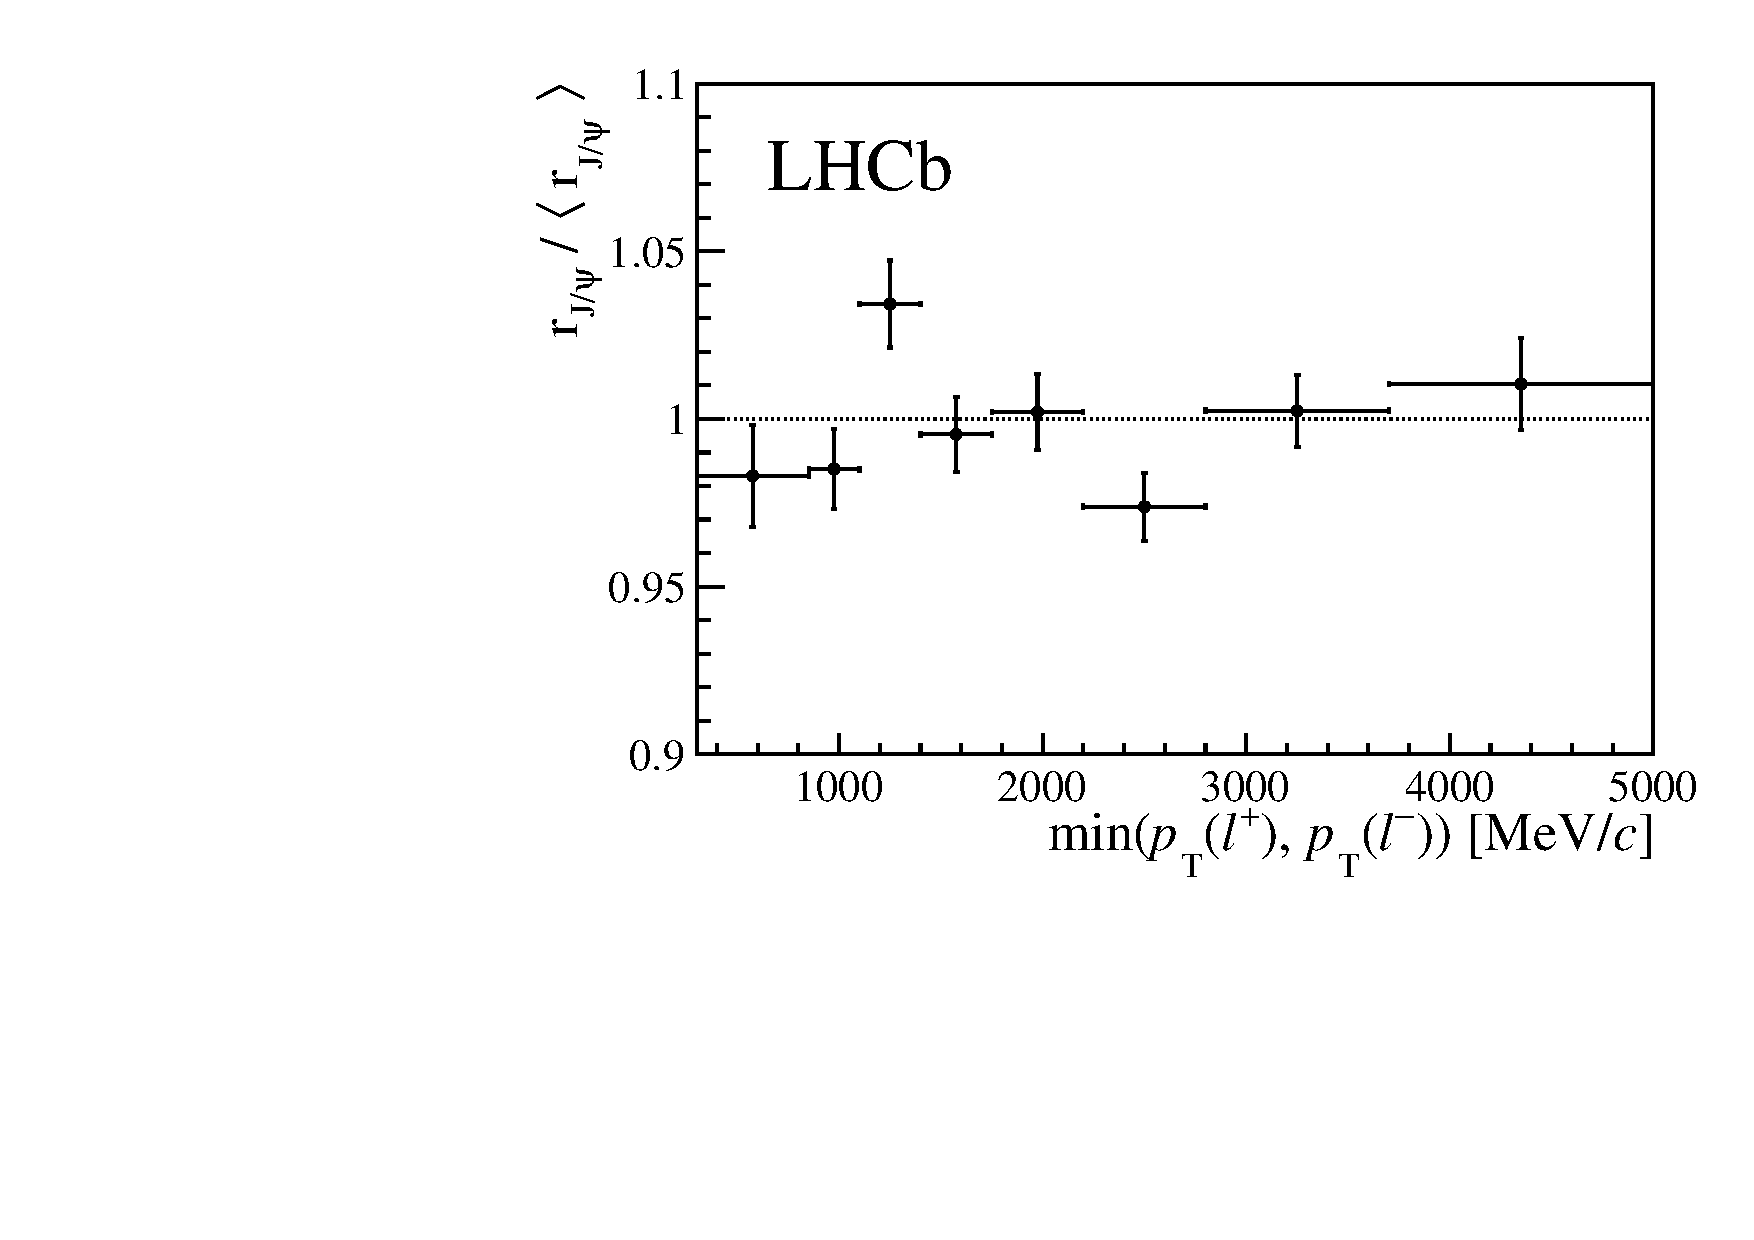
\includegraphics[width=0.45\linewidth,trim={0 0 0 0.5cm}, clip]{figures/Fig9d.pdf}
      \end{center}
     \caption{Differential \rjpsi measurement. (Top) distributions of the reconstructed spectra of (left) the angle between the leptons, and (right) the minimum \pt of the leptons. (Bottom) the single ratio \rjpsi relative to its average value $\left< \rjpsi \right>$ as a function of these variables. In the electron minimum \pt spectra, the structure at 2800\mevc is related to the trigger threshold.}
    \label{fig:rjpsi_differential1}
\end{figure}


\begin{figure}[!htbp]
   \begin{center}
   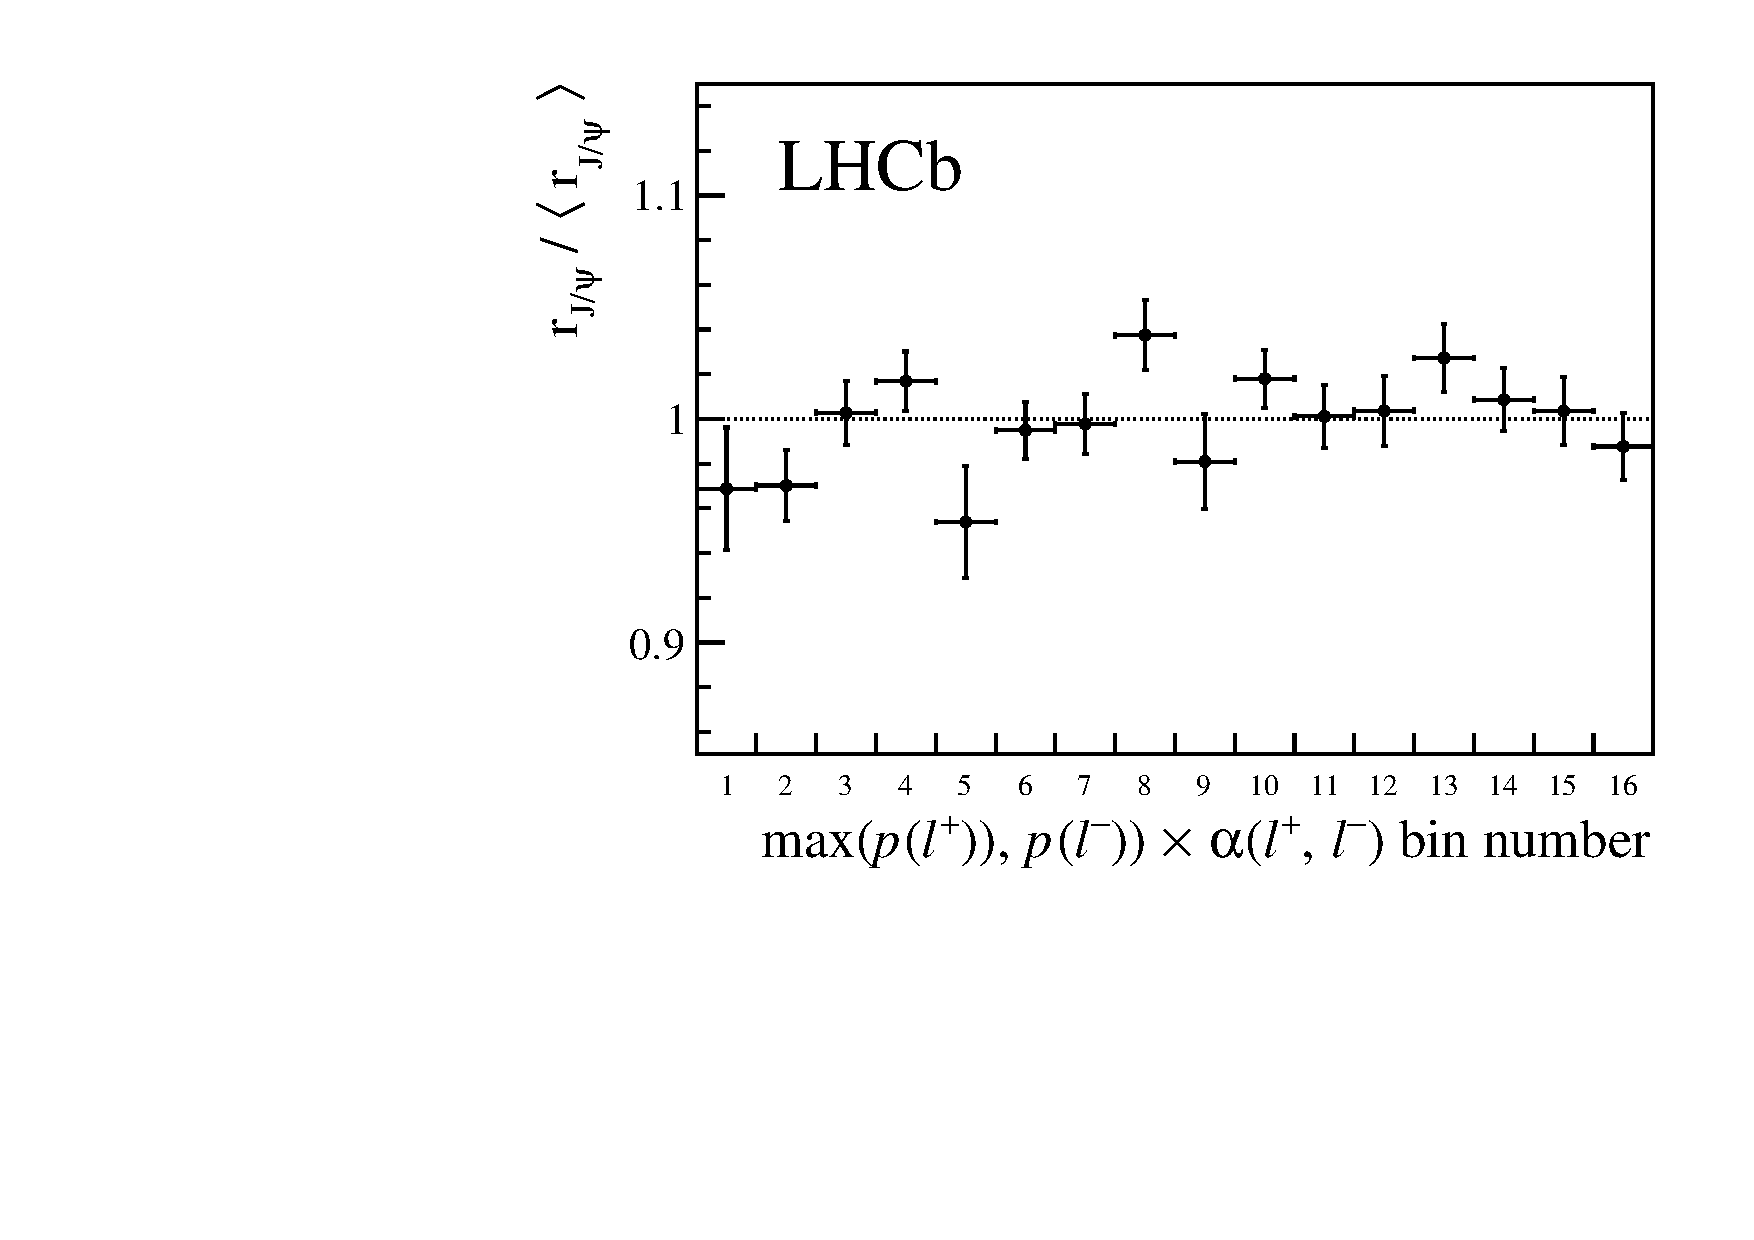
\includegraphics[width=0.45\linewidth]{figures/Fig10a.pdf}
    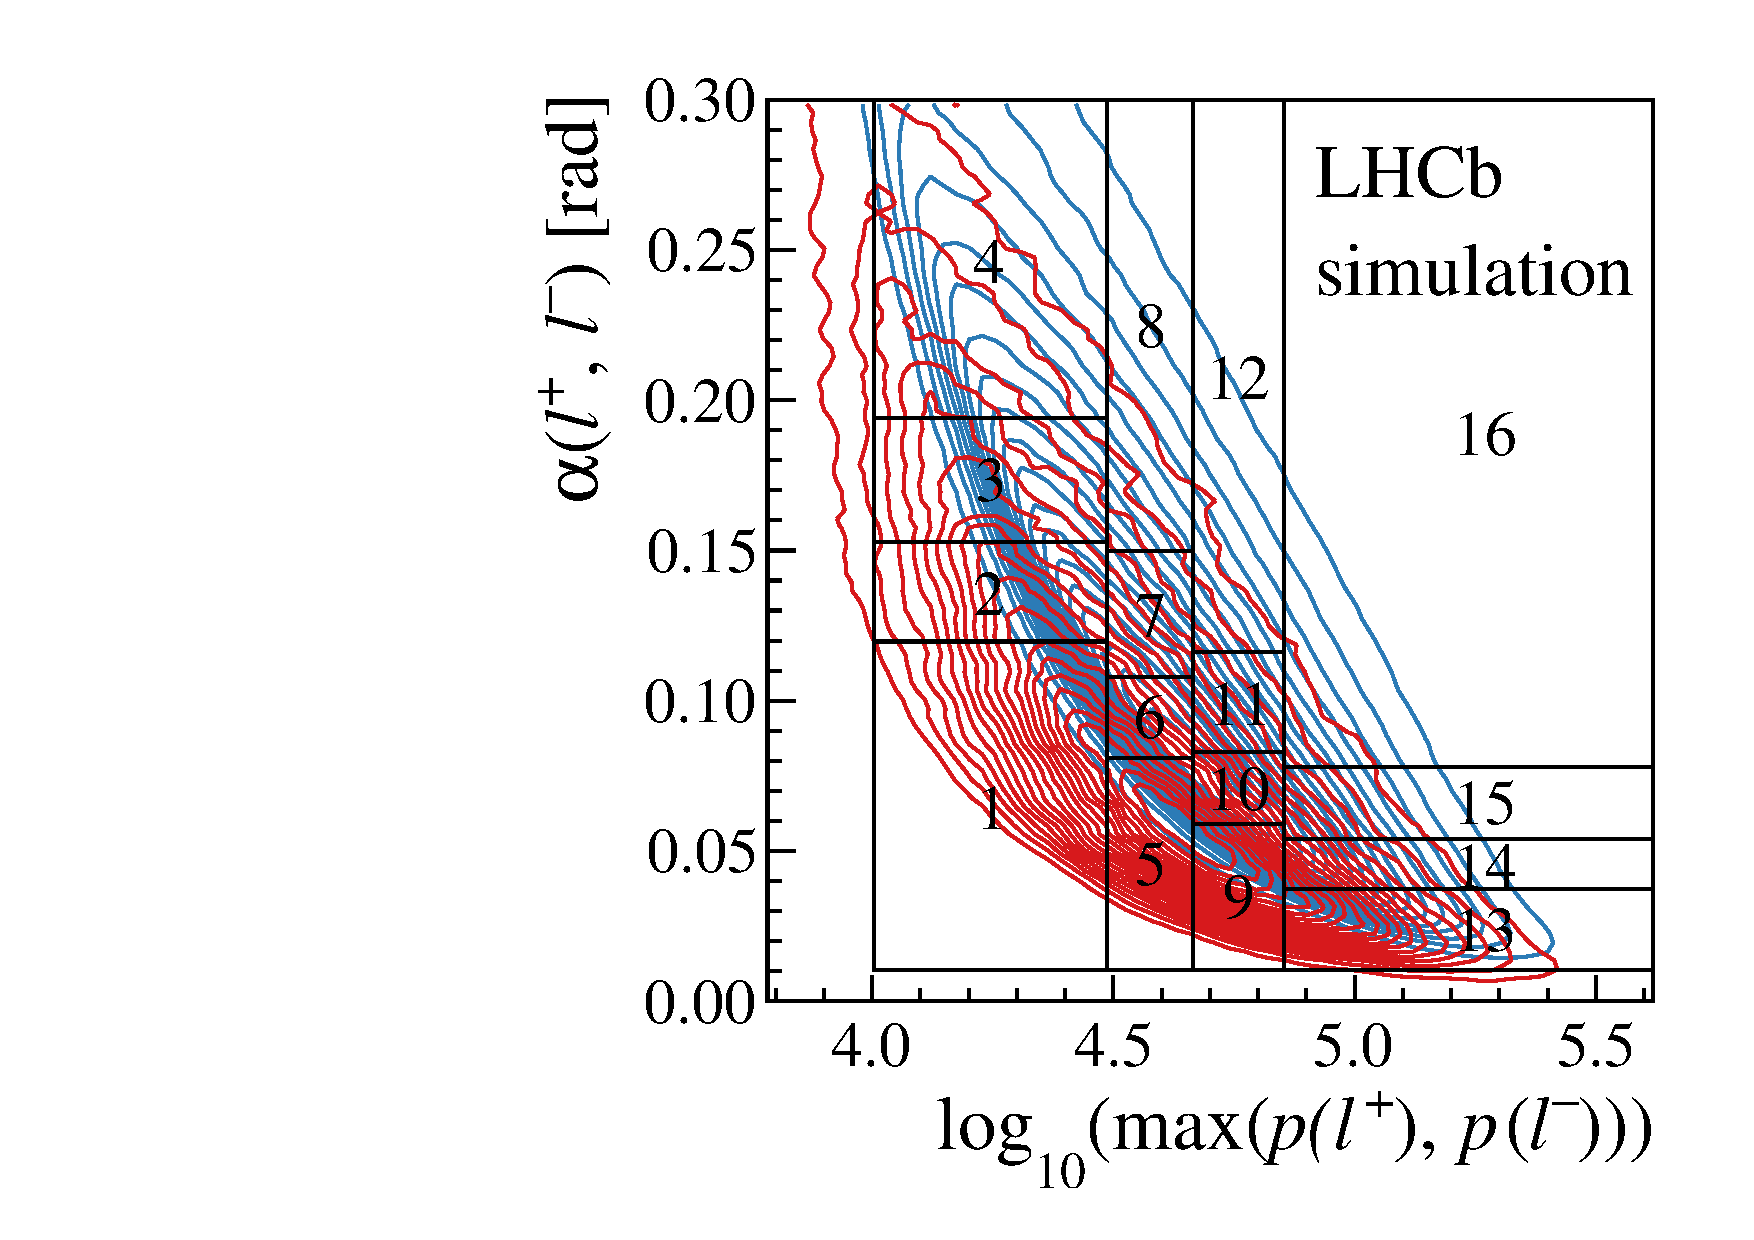
\includegraphics[height=0.32\linewidth]{figures/Fig10b.pdf}
   \end{center}
     \caption{Double differential \rjpsi measurement. (Left) the value of \rjpsi, relative to the average value of \rjpsi, measured in two-dimensional bins of the maximum lepton momentum, $p(l)$, and the opening angle between the two leptons, $\alpha(l^+,l^-)$. (Right) the bin definition in this two-dimensional space together with the
     distribution for \BuKee (\BuJpsiKee) decays depicted as red (blue) contours.}
    \label{fig:rjpsi_bin}
\end{figure}




\subsubsection*{Systematic uncertainties}

The majority of the sources of systematic uncertainty affect the relative efficiencies between nonresonant and resonant decays. These are included in the fit to \RK by allowing the relative efficiency to vary within Gaussian constraints. The width of the constraint is determined by adding the contributions from the different sources in quadrature. Correlations in the systematic uncertainties between different trigger categories and run periods are taken into account. Systematic uncertainties affecting the determination of the signal yield are assessed using pseudoexperiments generated with variations of the fit model. Pseudoexperiments are also used to assess the degree of bias originating from the fitting procedure. The bias is found to be 1\% of the statistical precision, \ie negligible with respect to other sources of systematic uncertainty.

For the nonresonant \BuKee decays, the systematic uncertainties are dominated by the modelling of the signal and background components used in the fit. The effect is at the 1\% level. A significant proportion (0.7\%) of this  uncertainty comes from the limited knowledge of the $K\pi$ spectrum in \BuBdKpiplusee decays. In addition, a 0.2\% systematic uncertainty is assigned for the potential contribution from \BuBdKpipiplusee events. 
A comparable uncertainty to that from the modelling of the signal and background components is induced by the limited sizes of calibration samples. Other sources of systematic uncertainty, such as the calibration of \Bu production kinematics, the trigger calibration and the determination of the particle identification efficiencies, contribute at the few-permille or permille level, depending strongly on the data-taking period and the trigger category. 


% The effect on \RK is at the $\pm0.008$ level. A  comparable uncertainty arises from the limited size of the calibration samples, with negligible contributions from the calibration of \Bu production kinematics and modelling of the selection and particle identification efficiencies. 

The uncertainties on parameters used in the simulation model of the signal decays affect the \qsq distribution and hence the selection efficiency. These uncertainties are propagated to an uncertainty on \RK using predictions from the {\sc{flavio}} software package~\cite{Straub:2018kue} but give rise to a negligible effect. Similarly, the differing \qsq resolution between data and simulation, which alters estimates of the \qsq migration, has negligible impact on the result.


\chapter{Additional experimental results\label{chap:Experimental-results} }

\addcontentsline{lof}{chapter}{Experimental results\lofpost}  
\addcontentsline{lot}{chapter}{Experimental results\lofpost}

\singlespacing 
\epigraph{
A strong claim of violation [of Bell's inequality] should be supported by at least a 5 sigma deviation.}
{Alain Aspect\\Rosenthal Lecture, 2018} 
\doublespacing\noindent \noindent\lettrine{T}{his} chapter presents experimental results
and control experiments that support the main experimental results
and conclusions presented in Chapter~\ref{chap:Introduction-and-overview}.
The characterization of the Hamiltonian parameters, coherence properties,
and other non-idealities of the two-transmon, one-readout-cavity device
employed in the experiment is discussed in Sec.~\ref{sec:Characterization-of-the}.
The calibration  of the tomography and control pulses and relevant
control experiments are discussed in Sec.~\ref{sec:Control-of-the}.
A summary of the  drive amplitudes and frequencies can be found in
Sec.~\ref{subsec:Atom-and-cavity}. Details of the experimental flow
of the catch and reverse protocol with regard to the FPGA controller
are discussed in Sec.~\ref{sec:Catching-and-reversing}. A comparison
between the predictions of the quantum trajectory description of the
experiment developed in Chapter~\ref{chap:theoretical-description-jumps}
and the main experimental results is presented in Sec.~\ref{subsec:Comparison-between-theory}.

\section{Characterization of the system\label{sec:Characterization-of-the}}

In this section, we describe the characterization of the Hamiltonian
and coherence parameters of the two-transmon, one-readout-cavity device
employed in the experiment. In reference to the protected Dark level,
which is engineered to be decoupled from the environment and readout
cavity, we  nickname the device ``Darkmon.''  The low-excitation
manifold of the Darkmon device is well described by the approximate
dispersive Hamiltonian, see Sec.~\ref{sec:circuit-design}, 
\begin{align}
\hat{H}/\hbar= & \omega_{\mathrm{B}}\hat{b}^{\dagger}\hat{b}-\frac{1}{2}\alpha_{\mathrm{B}}\hat{b}^{\dagger2}\hat{b}^{2}+\omega_{\mathrm{D}}\hat{d}^{\dagger}\hat{d}-\frac{1}{2}\alpha_{\mathrm{D}}\hat{d}^{\dagger2}\hat{d}^{2}-\chi_{\mathrm{DB}}\hat{b}^{\dagger}\hat{b}\hat{d}^{\dagger}\hat{d}\label{eq:Hamiltonian-of-sys}\\
 & \left(\omega_{\mathrm{C}}+\chi_{\mathrm{B}}\hat{b}^{\dagger}\hat{b}+\chi_{\mathrm{D}}\hat{d}^{\dagger}\hat{d}\right)\hat{c}^{\dagger}\hat{c}\,,\nonumber 
\end{align}
where $\omega_{\mathrm{D,B,C}}$ are the Dark, Bright, and cavity
mode frequencies, $\hat{d}$, $\hat{b},$ $\hat{c}$ are the respective
mode amplitude (annihilation) operators, $\alpha_{{\rm D}}$ ($\alpha_{{\rm B}}$)
is the Dark (Bright) transmon anharmonicity, $\chi_{\mathrm{D}}$
($\chi_{\mathrm{B}}$) is the dispersive shift between the Dark (Bright)
transmon and the readout cavity, and $\chi_{\mathrm{DB}}$ is the
dispersive shift between the two qubits. The Dark, $\ket{\mathrm{D}}$,
and Bright, $\B,$ states correspond to a single excitation in the
Dark and Bright transmon modes, $\hat{d}^{\dagger}\ket0$ and $\hat{b}^{\dagger}\ket0$,
respectively; see Fig.~\ref{fig:Darkmon-energy-level-diagram} for
a level diagram of the low-energy manifold. 

The readout cavity frequency was spectroscopically measured in reflection
\citep{Geerlings2013}, $\omega_{\mathrm{C}}/2\pi=8979.640\text{\,MHz}$,
and the extracted cavity linewidth agreed well with an independent
measurement of the energy-relaxation rate of the cavity extracted
from a time-domain ring-down measurement, $\kappa/2\pi=3.62\pm0.05\,\mathrm{MHz}.$
The cavity was observed to be well over-coupled; i.e., the coupling
quality factor, $Q_{c}$, dominated the internal quality factor, $Q_{i}$;
making it difficult to precisely extract $Q_{i}.$ The frequency and
anharmonicity of the B transmon were $\omega_{\mathrm{B}}/2\pi=5570.349\,\mathrm{MHz}$
and $\alpha_{\mathrm{B}}/2\pi=195\,\mathrm{MHz}$, respectively, measured
with two-tone pulsed spectroscopy \citep{Geerlings2013,Reagor2016}.
The frequency and anharmonicity of the D transmon, $\omega_{\mathrm{D}}/2\pi=4845.255\,\mathrm{MHz}$
and $\alpha_{\mathrm{D}}/2\pi=152\,\mathrm{MHz}$, respectively, were
measured in a modified two-tone spectroscopy sequence, where the $\G$
level was mapped to the $\B$ level at the end of the spectroscopy
sequence, before the readout, with $\pi$-pulse on the BG transition.
In a similar two-tone spectroscopy experiment, which included a pre-rotation
on either the BG or DG transition, and a measurement rotation after
the probe tone is turned off but before the readout tone is actuated,
the cross-Kerr coupling between the two qubits was measured to be
$\chi_{\mathrm{DB}}/2\pi=61\pm2\,\mathrm{MHz}$. In a standard energy-relaxation
experiment \citep{Geerlings2013}, the $\ket{\mathrm{B}}$ lifetime
was measured to be $T_{\mathrm{1}}^{\mathrm{B}}=28\pm2\,\mathrm{\mu s}$,
which we believe is limited by the Purcell effect with the readout
cavity mode, based on a finite-element calculation, see Sec.~\ref{subsec:Calculation-of-EPR}.
The Ramsey coherence time of $\B$ was $T_{\mathrm{2}}^{\mathrm{R,B}}=18\pm1\,\mathrm{\mu s}$,
possibly limited by photon shot noise \citep{Gambetta2006-dephasing,Rigetti2012}.
The measured Hamiltonian and coherence parameters of the device are
summarized in Table~\ref{tab:system-params}, where the drive parameters
employed in the experiment can also be found. 

\begin{table}
\begin{centering}
\renewcommand*\arraystretch{1.5}
\hspace*{-1.2cm} % manually align to center of page 
\begin{tabular}{rl|rl|rl}
\multicolumn{2}{c|}{\textbf{Readout cavity}} & \multicolumn{2}{c|}{\textbf{BG transition}} & \multicolumn{2}{c}{\textbf{DG transition}}\tabularnewline
\hline 
\hline 
\multicolumn{6}{c}{\textbf{\rule{0pt}{5ex}Mode frequencies and non-linear parameters}}\tabularnewline
\hline 
\textbf{\rule{0pt}{4ex}}$\omega_{\mathrm{C}}/2\pi=$ & $8979.640\text{\,MHz}$ & ~$\omega_{\mathrm{BG}}/2\pi=$ & $5570.349\text{\,MHz}$ & ~$\omega_{\mathrm{DG}}/2\pi=$ & $4845.255\text{\,MHz}$\tabularnewline
 &  & $\chi_{\mathrm{B}}/2\pi=$ & $-5.08\pm0.2\,\mathrm{MHz}$~ & $\chi_{\mathrm{D}}/2\pi=$ & $-0.33\pm0.08\,\mathrm{MHz}$\tabularnewline
 &  & $\alpha_{\mathrm{B}}/2\pi=$ & $195\pm2\,\mathrm{MHz}$ & $\alpha_{\mathrm{D}}/2\pi=$ & $152\pm2\,\mathrm{MHz}$\tabularnewline
 &  & \multicolumn{4}{c}{$\chi_{\mathrm{DB}}/2\pi=61\pm2\,\mathrm{MHz}$}\tabularnewline
\multicolumn{6}{c}{\textbf{\rule{0pt}{5ex}Coherence related parameters}}\tabularnewline
\hline 
\textbf{\rule{0pt}{5ex}}$\kappa/2\pi$= & $3.62\pm0.05\,\mathrm{MHz}$ & $T_{\mathrm{1}}^{\mathrm{B}}=$ & $28\pm2\,\mathrm{\mu s}$ & $T_{\mathrm{1}}^{\mathrm{D}}=$ & $116\pm5\,\mathrm{\mu s}$\tabularnewline
$\eta=$ & $0.33\pm0.03$ & $T_{\mathrm{2\mathrm{R}}}^{\mathrm{B}}=$ & $18\pm1\,\mathrm{\mu s}$ & $T_{\mathrm{2\mathrm{R}}}^{\mathrm{D}}=$ & $120\pm5\,\mathrm{\mu s}$\tabularnewline
$T_{\mathrm{int}}=$ & $260.0\,\mathrm{ns}$ & $T_{\mathrm{2\mathrm{E}}}^{\mathrm{B}}=$ & $25\pm2\,\mathrm{\mu s}$ & $T_{\mathrm{2\mathrm{E}}}^{\mathrm{D}}=$ & $162\pm6\,\mathrm{\mu s}$\tabularnewline
$n_{\mathrm{th}}^{\mathrm{C}}\le$ & $0.0017\pm0.0002$ & $n_{\mathrm{th}}^{\mathrm{B}}\le$ & $0.01\pm0.005$ & $n_{\mathrm{th}}^{\mathrm{D}}\leq$ & $0.05\pm0.01$\tabularnewline
\multicolumn{6}{c}{\textbf{\rule{0pt}{5ex}Drive amplitude and detuning parameters}}\tabularnewline
\hline 
\textbf{\rule{0pt}{5ex}}$\bar{n}=$ & $5.0\pm0.2$ & ~$\Omega_{\mathrm{B}0}/2\pi=$ & $1.20\pm0.01\,\mathrm{MHz}$ & ~$\Omega_{\mathrm{DG}}/2\pi=$ & $20\pm2\,\mathrm{kHz}$\tabularnewline
 &  & ~$\Omega_{\mathrm{B}1}/2\pi=$ & $0.60\pm0.01\,\mathrm{MHz}$ &  & \tabularnewline
$\Delta_{\mathrm{R}}=$ & $\chi_{\mathrm{B}}$ & ~$\Delta_{\mathrm{B}1}/2\pi=$ & $-30.0\,\text{MHz}$ & ~$\Delta_{\mathrm{DG}}/2\pi=$ & $-275.0\,\text{kHz}$\tabularnewline
\end{tabular}
\par\end{centering}
\caption[Compilation of experimental parameters]{\textbf{\label{tab:system-params}Compilation of  experimental parameters.}}
\end{table}


\subsection{Measurement-induced relaxation\textit{ $T_{1}(\bar{n})$\label{subsec:Measurement-induced-relaxation}}}

It has been established in the superconducting qubit community \citep{Boissonneault2009-Photon-induced-relax,Slichter2012,Sank2016-T1vsNbar,Slichter2016-T1vsNbar}
that as a function of the number of photons circulating in the readout
cavity, $\bar{n},$ the energy-relaxation time, $T_{1}$, of a dispersively
coupled qubit is degraded. In Fig.~\ref{fig:T1-vs-nbar}, we show
a measurement of the $T_{1}$ lifetime of the $\B$ and $\D$ states
as a function of the readout drive strength, in units of the number
of circulating photons, $\bar{n}$, when the drive is resonant; the
measurement protocol is explained in the figure caption. As typically
observed in cQED experiments, the Bright level, which is directly
coupled to the readout cavity, exhibits a large parasitic measurement-induced
energy relaxation, $T_{1}^{\mathrm{B}}\left(\bar{n}\right)$ -- its
lifetime suffers more than an order of magnitude degradation. On the
other hand, perhaps surprisingly, the lifetime, $T_{1}^{\mathrm{D}},$
of the Dark state, $\ket{\mathrm{D}}$, remains essentially unaffected,
even at very large drive strengths, $\bar{n}\approx50$. In this sense,
the Dark level is protected from the $T_{1}\left(\bar{n}\right)$
parasitic effect.

\begin{figure}
\begin{centering}
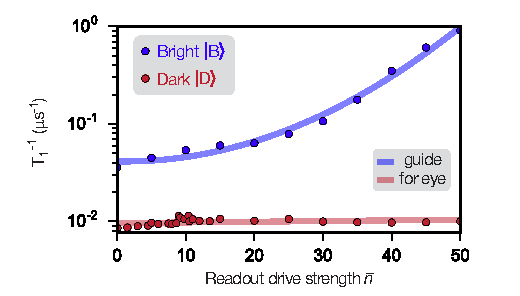
\includegraphics[scale=1.5]{results/T1-vs-nbar}
\par\end{centering}
\caption[Measurement-induced energy relaxation $T_{1}(\bar{n})$]{\label{fig:T1-vs-nbar}\textbf{Measurement-induced energy relaxation
$T_{1}(\bar{n})$.} Energy relaxation rate ($T_{1}^{-1}$) of $\ket{\mathrm{B}}$
(blue dots) and $\ket{\mathrm{D}}$ (red dots) as a function of $\bar{n}$,
measured with the following protocol: after the atom is prepared in
either $\ket{\mathrm{B}}$ or $\ket{\mathrm{D}}$, the readout tone
($\mathrm{R}$) is turned on for duration $t_{\mathrm{read}}$ with
amplitude $\bar{n}$ (corresponding to the number of steady-state
photons in the readout cavity when excited on resonance), whereafter,
the population of the initial state is measured. As in all other experiments,
the readout drive is applied at the $\ket{\mathrm{B}}$ cavity frequency
($\omega_{\mathrm{C}}-\chi_{\mathrm{B}}$). The relaxation rates are
extracted from exponential fits of the population decay as a function
of $t_{\mathrm{read}}$, from $1.3\times10^{7}$ experimental realizations.
The solids lines are guides to the eye: blue line indicates the rapid
degradation of $T_{1}^{\mathrm{B}}$ as a function of the readout
strength, while the red line indicates the nearly constants $T_{1}^{\mathrm{D}}$
of the protected dark level.}
\end{figure}


\section{Control of the three-level atom\label{sec:Control-of-the}}

\subsection{Qubit pulses\label{subsec:Qubit-pulses-calib}}

The implementation of precise and coherent manipulation of the three-level
atom is important for the tomographic reconstruction of the flight
of the quantum jump as well the ability to faithfully reverse it.
One of the main sources of pulse infidelity is typically decoherence,
but the rather long coherence time of the Darkmon device relative
to the duration of the pulses employed in the experiment make it largely
unimportant, and instead, place emphasis on the technical details
of pulse generation and Hamiltonian non-idealities, such as leakage
to higher excited states. 

Mitigation of main technical non-idealities. The effect of the zero-order
hold of the FPGA digital-to-analog converter (DAC) was mitigated by
installing a 270~MHz low pass filter (\textit{Mini-Circuits BLP-300+})
on each of the analog output channels, see Sec.~\ref{sec:Microwave-setup}.
All microwave tones were generated with single-sideband IQ-controlled
modulation at a base intermediate frequency (IF) of 50~MHz, and the
lower radio-frequency (RF) sideband was used for the control tones
(detuned 50~MHz below the local oscillator (LO) frequency). The IQ
mixers were calibrated with a four stage iterative routine to minimize
carrier leakage, by tuning the DC offsets of the I and Q channels,
and to suppress the RF image, by minimizing the quadrature skew and
IQ gain imbalance. The LO leakage could typically be suppressed to
$\approx-70$~dB relative to the RF tone. Spurious intermodulation
tones generated by higher-order non-linear terms present in the mixers
{[}i.e., third-order intercept-point (IP3) products{]} were generally
negligible as the mixers were not typically driven near saturation,
but bandpass filters were installed on the RF outputs of all mixers
to nonetheless suppress any spurious tones. Excess noise from the
following RF amplifier (\textit{MiniCircuits ZVA-183-S+}) was suppressed
by 80\,dB when the control drives were turned off by use of a high-isolation
SPST switch (\textit{Analog Device HMC-C019}).

The pulses applied to the Dark and Bright transition were calibrated
with a combination of Rabi, derivative removal via adiabatic gate
(DRAG) \citep{JChow2010-DRAG}, \emph{All-XY} \citep{Reed2013}, and
amplitude pulse train sequences \citep{Bylander2011}. Pulse timings
and delays, especially between the analog channels and the SPST switch
digital markers, were calibrated with a wide-bandwidth oscilloscope
with ultra-low jitter (\emph{Keysight 86100D Infiniium DCA-X}). The
alignment was verified by performing a Gaussian qubit $\pi$ pulse
on the GB transition and varying the delay between the rise of the
SPST digital marker and the signal on the analog IQ pair playing the
pulse. 


\subsection{Tomography of the three-level atom\label{subsec:Tomography-of-three-level}}

At the end of each experimental realization, we performed one of 15
rotation sequences on the atom that transferred information about
one component of the density matrix, $\hat{\rho}_{a}$, to the population
of $\ket{\mathrm{B}}$, which was measured with a 600~ns square pulse
on the readout cavity. Pulses were calibrated as discussed in Sec.~\ref{subsec:Qubit-pulses-calib}.
The readout signal was demodulated with the appropriate digital filter
function required to realize temporal mode matching \citep{Eichler2012-itinerant-entanglement}.
To remove the effect of potential systematic offset errors in the
readout signal, we subtracted the measurement results of operator
components of $\hat{\rho}_{a}$ and their opposites. From the measurement
results of this protocol, we reconstructed the density matrix $\hat{\rho}_{a}$,
and subsequently parametrized it the useful form 
\begin{equation}
\hat{\rho}_{a}=\begin{pmatrix}\frac{N}{2}\left(1-Z_{\mathrm{GD}}\right) & \frac{N}{2}\left(X_{\mathrm{GD}}+iY_{\mathrm{GD}}\right) & R_{\mathrm{BG}}+iI_{\mathrm{BG}}\\
\frac{N}{2}\left(X_{\mathrm{GD}}-iY_{\mathrm{GD}}\right) & \frac{N}{2}\left(1+Z_{\mathrm{GD}}\right) & R_{\mathrm{BD}}+iI_{\mathrm{BD}}\\
R_{\mathrm{BG}}-iI_{\mathrm{BG}} & R_{\mathrm{BD}}-iI_{\mathrm{BD}} & 1-N
\end{pmatrix},\label{eq:rhoa}
\end{equation}
where $X_{\mathrm{GD}},Y_{\mathrm{GD}},$ and $Z_{\mathrm{GD}}$ are
the Bloch vector components of the GD manifold, $N$ is the total
population of the $\ket{\mathrm{G}}$ and $\ket{\mathrm{D}}$ states,
while $R_{\mathrm{BG}},R_{\mathrm{BD}},I_{\mathrm{BG}}$ and $I_{\mathrm{BD}}$
are the coherences associated with $\ket{\mathrm{B}}$, relative to
the GD manifold. The measured population in $\ket{\mathrm{B}}$, $1-N$,
remains below 0.03 during the quantum jump, see Fig.~\ref{fig:tomo_tmid}.
Tomographic reconstruction was calibrated and verified by preparing
Clifford states, accounting for the readout fidelity of 97\%.

\paragraph{Control experiment.}

In Fig.~\ref{fig:time-resolved-tomo-D}, we show the results of a
control experiment where we verified the Ramsey coherence ($T_{\mathrm{2R}}^{\mathrm{D}}$)
and energy relaxation ($T_{\mathrm{1}}^{\mathrm{D}}$) times of the
DG transition with our tomography method. Solid lines are fitted theoretical
curves for the free evolution of the prepared initial state $\frac{1}{\sqrt{2}}\left(\D-\G\right)$.
The $T_{\mathrm{2R}}^{\mathrm{D}}=119.2\,\mathrm{\mu s}$ value gained
from the simultaneous fit of $X_{\mathrm{DG}}(t)$ and $Y_{\mathrm{DG}}(t)$
matches the lifetime independently obtained from a standard $T_{\mathrm{2R}}$
measurement. Similarly, the value of $T_{\mathrm{1}}^{\mathrm{D}}=115.4\,\mathrm{\mu s}$
extracted from an exponential fit of $Z_{\mathrm{DG}}(t)$ matches
the value obtained from a standard $T_{\mathrm{1}}$ measurement.
We note that our tomography procedure is well calibrated and skew-free,
as evident in the zero steady-state values of $X_{\mathrm{DG}}$ and
$Y_{\mathrm{DG}}$. The steady state $Z_{\mathrm{DG}}$ corresponds
to the thermal population of the dark state $n_{\mathrm{th}}^{\mathrm{D}}$.
It has recently been shown that residual thermal populations in cQED
systems can be significantly reduced by properly thermalizing the
input-output lines \citep{Yeh2017Atten,Wang2019-cav-atten}.

\begin{figure}
\begin{centering}
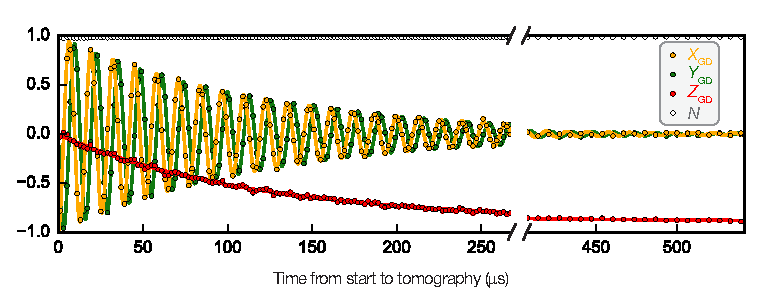
\includegraphics[scale=1.2]{results/time-resolved-tomo-D}
\par\end{centering}
\caption[Control experiment: time-resolved tomogram of the free evolution of
a DG superposition]{\label{fig:time-resolved-tomo-D}\textbf{Control experiment: time-resolved
tomogram of the free evolution of a DG superposition. }The atom is
prepared in $\frac{1}{\sqrt{2}}\left(\D-\G\right)$ and tomography
is performed after a varied delay. Dots: reconstructed conditional
GD tomogram ($X_{\mathrm{DG}},Y_{\mathrm{DG}}$, and $Z_{\mathrm{DG}}$)
and population in DG manifold, $N$, see Eq.~(\ref{eq:rhoa}). Solid
lines: theoretical fits. }
\end{figure}


\paragraph{Mid-flight tomogram.}

In the presence of the coherent Rabi drive $\Odg$ (corresponding
to catch parameter $\Delta t_{\mathrm{off}}=0$), the complete tomogram
of the three-level atom was reconstructed, and a slice at the mid-flight
time, $\Delta t_{\mathrm{mid}}$, is shown in Fig.~\ref{fig:tomo_tmid}.
All imaginary components of the reconstructed conditional density
matrix, $\rho_{\mathrm{c}}$, are negligibly small, less than 0.007,
as expected, see Sec.~\ref{subsec:Comparison-between-theory}, for
well-calibrated tomographic phase control. The population of the $\B$
state, 0.023, is nearly negligible as well, as it is conditioned away
by the IQ filter, see Sec.~\ref{subsec:IQ-filter}.
\begin{figure}
\centering{}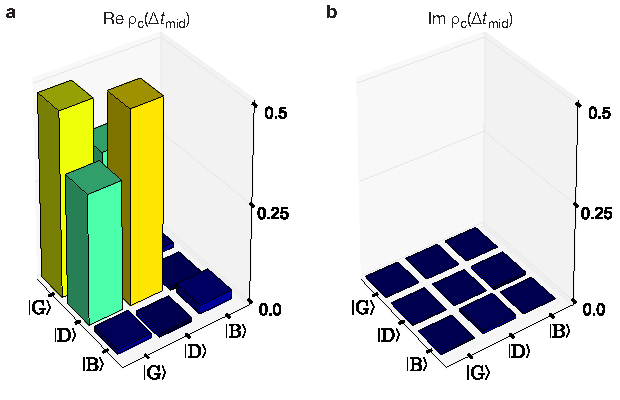
\includegraphics[width=120mm]{results/tomogram_tmid}
\caption[Mid-flight tomogram]{\label{fig:tomo_tmid}\textbf{Mid-flight tomogram. }The plots show
the real (a) and imaginary (b) parts of the conditional density matrix,
$\rho_{\mathrm{c}}$, at the mid flight of the quantum jump ($\Delta t_{\mathrm{catch}}=\Delta t_{\mathrm{mid}}$),
in the presence of the Rabi drive from $\ket{\mathrm{G}}$ to $\ket{\mathrm{D}}$
($\Delta t_{\mathrm{off}}=0$). The population of the $\ket{\mathrm{B}}$
state is 0.023, and the magnitude of all imaginary components is less
than 0.007. }
\end{figure}


\subsection{Atom and cavity drives \label{subsec:Atom-and-cavity}}

In all experiments, unless noted otherwise, the following drive parameters
were used: The DG Rabi drive, $\Omega_{\mathrm{DG}}$, was applied
275~kHz below $\omega_{\mathrm{D}}$ to account for the Stark shift
of the cavity. The BG drive, $\Omega_{\mathrm{BG}}$, was realized
as a bi-chromatic tone in order to unselectively address the BG transition,
which was broadened and Stark shifted due to the coupling between
$\ket{\mathrm{B}}$ and the readout cavity. Specifically, we addressed
transitions from $\ket{\mathrm{G}}$ to $\ket{\mathrm{B}}$ with a
Rabi drive $\Omega_{\mathrm{B0}}/2\pi=1.20\pm0.01\,$~MHz at frequency
$\omega_{\mathrm{BG}}$, whereas transitions from $\ket{\mathrm{B}}$
to $\ket{\mathrm{G}}$ were addressed with a Rabi drive $\Omega_{\mathrm{B1}}/2\pi=0.60\pm0.01\,$~MHz
tuned 30~MHz below $\omega_{\mathrm{BG}}$. This bi-chromatic scheme
provided the ability to tune the up-click and down-click rates independently,
but otherwise essentially functioned as an incoherent broad-band source.
In Table~\ref{tab:Summary-of-timescales.}, we summarize the hierarchy
of timescales established by the drive amplitudes and frequencies
as well as the relevant decoherence properties of the atom.

\begin{table}[!ht]
\begin{centering}
\addtolength{\tabcolsep}{2pt} 
\renewcommand*{\arraystretch}{1.5}
 %
\begin{tabular}{cc>{\raggedright}p{0.65\columnwidth}}
\hline 
\textbf{Symbol}  & \textbf{Value}  & \textbf{Description}\tabularnewline
\hline 
$\Gamma^{-1}$  & $\approx8.8$\,ns  & Effective measurement time of $\ket{\mathrm{B}}$, approximately given
by $1/\kappa\bar{n}$, where $\bar{n}=5\pm0.2$ in the main experiment\tabularnewline
$\kappa^{-1}$  & $44.0\pm0.06$\,ns  & Readout cavity lifetime\tabularnewline
$T_{\mathrm{int}}$  & 260.0\,ns  & Integration time of the measurement record, set in the controller
at the beginning of the experiment \tabularnewline
$\Gamma_{\mathrm{BG}}^{-1}$  & $0.99\pm0.06\,\mathrm{\mu s}$  & Average time the atom rests in $\ket{\mathrm{G}}$ before an excitation
to $\ket{\mathrm{B}}$, see Fig.~\ref{fig:jumps}b\tabularnewline
$\Delta t_{\mathrm{mid}}$  & $3.95\,\mathrm{\mu s}$  & No-click duration for reaching $Z_{\mathrm{GD}}=0$ in the flight
of the quantum jump from $\ket{\mathrm{G}}$ to $\ket{\mathrm{D}}$,
in the full presence of $\Omega_{\mathrm{DG}}$, see Fig.~\ref{fig:catch}b\tabularnewline
$\Gamma_{\mathrm{GD}}^{-1}$  & $30.8\pm0.4\,\mathrm{\mu s}$  & Average time the atom stays in $\ket{\mathrm{D}}$ before returning
to $\ket{\mathrm{G}}$ and being detected, see Fig.~\ref{fig:jumps}b\tabularnewline
$T_{1}^{\mathrm{D}}$  & $116\pm5\,\mathrm{\mu s}$  & Energy relaxation time of $\ket{\mathrm{D}}$\tabularnewline
$T_{2\mathrm{R}}^{\mathrm{D}}$  & $120\pm5\,\mathrm{\mu s}$  & Ramsey coherence time of $\ket{\mathrm{D}}$\tabularnewline
$T_{2\mathrm{E}}^{\mathrm{D}}$  & $162\pm6\,\mathrm{\mu s}$  & Echo coherence time of $\ket{\mathrm{D}}$\tabularnewline
$\Gamma_{\mathrm{DG}}^{-1}$  & $220\pm5\,\mathrm{\mu s}$  & Average time between two consecutive $\ket{\mathrm{G}}$ to $\ket{\mathrm{D}}$
jumps\tabularnewline
\end{tabular}
\par\end{centering}
\caption[Summary of timescales]{\textbf{Summary of timescales. }List of the characteristic timescales
involved in the catch and reverse experiment. The Hamiltonian parameters
of the system are summarized in Sec.~\ref{sec:Characterization-of-the}.
\textbf{\label{tab:Summary-of-timescales.}}}
\end{table}


\section{Monitoring quantum jumps in real time }

\subsection{IQ filter \label{subsec:IQ-filter}}

To mitigate the effects of imperfections in the atom readout scheme
in extracting a $\ket{\mathrm{B}}$/not-$\ket{\mathrm{B}}$ result,
we applied a two-point, hysteretic IQ filter, implemented on the FPGA
controller in real time. The filter is realized by comparing the present
quadrature record values $\left\{ I_{\mathrm{rec}},Q_{\mathrm{rec}}\right\} $,
with three thresholds ($I_{\mathrm{B}},I_{\bar{\mathrm{B}}},$ and
$Q_{\mathrm{B}}$) in the following way: 
\begin{center}
\begin{tabular}{>{\raggedleft}m{20mm}|>{\centering}p{30mm}|>{\centering}p{30mm}|>{\centering}p{30mm}}
\textbf{Input: } & $Q_{\mathrm{rec}}\geq Q_{\mathrm{B}}$ or

$I_{\mathrm{rec}}>I_{\mathrm{B}}$  & $Q_{\mathrm{rec}}<Q_{\mathrm{B}}$ and

$I_{\mathrm{rec}}<I_{\bar{\mathrm{B}}}$  & $Q_{\mathrm{rec}}<Q_{\mathrm{B}}$ and

$I_{\bar{\mathrm{B}}}\leq I_{\mathrm{rec}}\leq I_{\mathrm{B}}$\tabularnewline
\hline 
\textbf{Output: } & $\ket{\mathrm{B}}$  & not-$\ket{\mathrm{B}}$  & previous\tabularnewline
\end{tabular}
\par\end{center}

\noindent The filter and thresholds were selected to provide a best
estimate of the time of a click, operationally understood as a change
in the filter output from $\ket{\mathrm{B}}$ to not-$\ket{\mathrm{B}}$.
The $I_{{\mathrm{B}}}$ and $I_{\bar{\mathrm{B}}}$ thresholds were
chosen 1.5 standard deviations away from the I-quadrature mean of
the $\ket{\mathrm{B}}$ and not-$\ket{\mathrm{B}}$ distributions,
respectively. The $Q_{{\mathrm{B}}}$ threshold was chosen 3 standard
deviations away from the Q-quadrature mean. Higher excited states
of the atom were selected out by $Q_{\mathrm{rec}}$ values exceeding
the $Q_{\mathrm{B}}$ threshold. 

\subsection{Unconditioned monitoring}

In Sec.~\ref{sec:Unconditioned-monitoring-of}, we described a protocol
for the unconditioned monitoring of the quantum jumps where the atom
is subject to the continuous Rabi drives $\Omega_{\mathrm{BG}}$ and
$\Omega_{\mathrm{DG}}$, as depicted in Fig.~\ref{fig:setup}. From
the continuous tracking of the quantum jumps, over 3.2~s. of data,
we histogrammed the times, $\tau_{\operatorname{not-B}}$, spent in
not-$\ket{\mathrm{B}}$, Fig.~\ref{fig:jumps}b. In Fig.~\ref{fig:B-wait-time},
we show the complimentary histogram for the times, $\tau_{{\rm B}},$
spent in $\B$, which is unlike the latter, in that it follows a single
exponential decay law. This single Poisson process character follows
from the fact that the $\B$ measurement result collapses the atom
to a single state, $\B$, unlike the not-$\B$ result. The average
time spent in $\B$, extracted from the fit, is $\bar{\tau}_{{\rm B}}=4.2\pm0.03\,\mathrm{\mu s}$.
\begin{figure}
\centering{}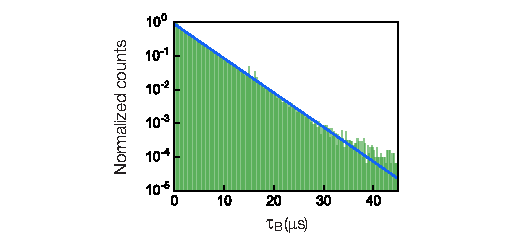
\includegraphics[width=145mm]{results/B_waiting_time}
\caption[Waiting time to switch from a $\B$ to not-$\B$ state assignment
result]{\label{fig:B-wait-time}\textbf{Waiting time to switch from a $\B$
to not-$\B$ state assignment result.} Semi-log plot of the histogram
(shaded green) of the duration of times corresponding to $\B$-measurement
results, $\tau_{\operatorname{B}}$, for 3.2~s of continuous data
of the type shown in Fig.~\ref{fig:jumps}a. Solid line is an exponential
fit, which yields a $4.2\pm0.03\,\mathrm{\mu s}$ time constant. }
\end{figure}

\pagebreak{}

\section{Catching and reversing the jump \label{sec:Catching-and-reversing}}

\subsection{Experiment flow}

\begin{figure}
\begin{centering}
%\hspace*{-1cm} % manually align to center of page 
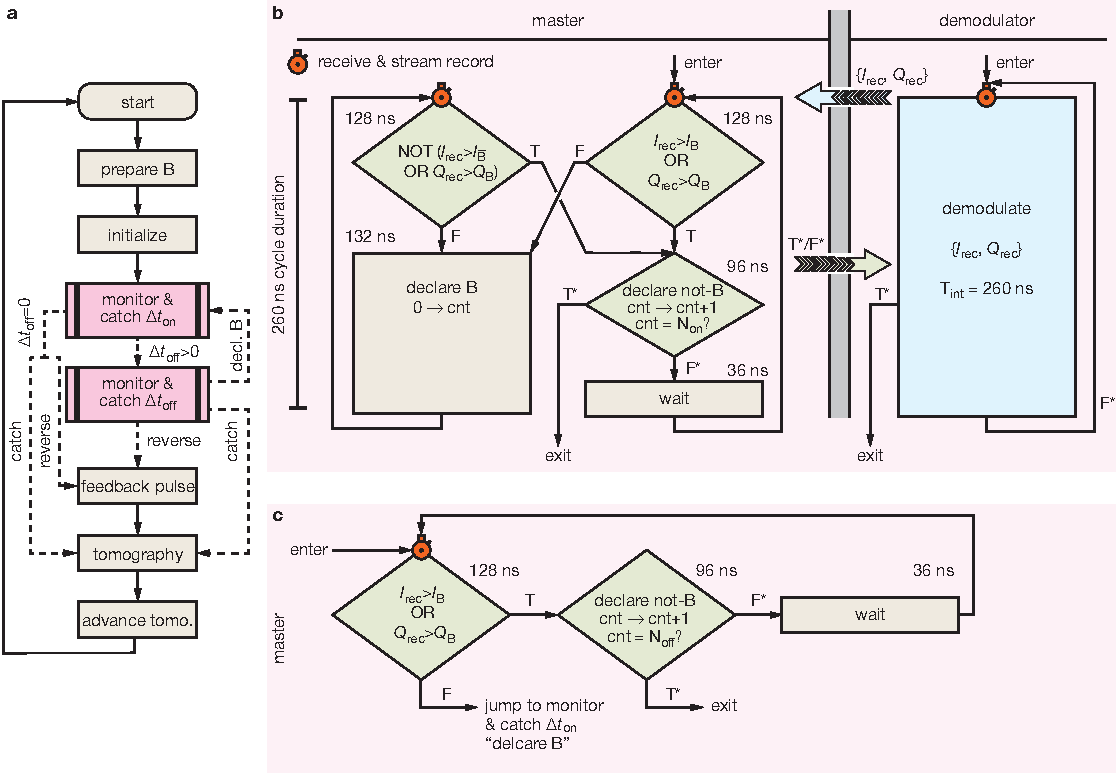
\includegraphics[angle=-90,scale=1.1]{results/experiment_flow}
\par\end{centering}
\caption[Experiment flow]{\label{fig:experiment-flow}\textbf{Experiment flow. }See text for
detailed description.}
\end{figure}
Figure \ref{fig:experiment-flow}a shows a flowchart representation
of steps involved in the catch and reverse protocol. In the following,
we describe each block in the diagram in the order in which it would
be executed.

\paragraph{Start:}

internal memory registers are set to zero \citep{Ofek2016,Liu2016Thesis},
including the no-click counter ``cnt,'' defined below. 

\paragraph{Prepare B:}

controller deterministically prepares the atom in $\ket{\mathrm{B}}$,
a maximally conservative initial state, with measurement-based feedback
\citep{Riste2012-qubit-measure-reset}. 

\paragraph{Initialize:}

controller turns on the atom ($\Omega_{\mathrm{BG}}$ and $\Omega_{\mathrm{DG}}$)
and cavity drives ($\mathrm{R}$) and begins demodulation. 

\paragraph{Monitor and catch $\Delta t_{\mathrm{on}}$: }

with all drives on ($\Omega_{\mathrm{BG}},\Omega_{\mathrm{DG}}$,
and $\mathrm{R}$), the controller actively monitors the cavity output
signal until it detects no-clicks for duration $\Delta t_{\mathrm{on}}$,
as described in panel (b), whereafter, the controller proceeds to
``monitor and catch $\Delta t_{\mathrm{off}}$'' in the case that
$\Delta t_{\mathrm{off}}>0$; otherwise, for $\Delta t_{\mathrm{off}}=0$,
the controller proceeds to ``tomography'' (``feedback pulse'')
for the catch (reverse) protocol.

\paragraph{Monitor and catch $\Delta t_{\mathrm{off}}$: }

with the Rabi drive $\Omega_{\mathrm{DG}}$ off, while keeping the
drives $\Omega_{\mathrm{BG}}$ and R on, the controller continues
to monitor the output signal. The controller exits the routine only
if it detects a click, proceeding to the ``declare B'' step of the
``monitor and catch $\Delta t_{\mathrm{on}}$'' routine, or if no
further clicks are detected for the pre-defined duration $\Delta t_{\mathrm{off}}$,
proceeding to ``tomography'' (``feedback pulse'') for the catch
(reverse) protocol.

\paragraph{Feedback pulse: }

with all the continuous drives turned off, the controller performs
a pulse on the DG transition of the atom, defined by the two angles
$\left\{ \theta_{I}\left(\Delta t_{\mathrm{catch}}\right),\varphi_{I}\left(\Delta t_{\mathrm{catch}}\right)\right\} $.

\paragraph{Tomography: }

controller performs next-in-order tomography sequence (see Sec.~\ref{subsec:Tomography-of-three-level})
while the demodulator finishes processing the final data in its pipeline.

\paragraph{Advance tomo.: }

tomography sequence counter is incremented, and after a $50~\mathrm{\mu s}$
delay, the next realization of the experiment is started.

\subsubsection{Logic and timing of catch subroutines}

\paragraph{Monitor and catch $\Delta t_{\mathrm{on}}$.}

Figure \ref{fig:experiment-flow}b shows a concurrent-programming
flowchart representation of the ``monitor and catch $\Delta t_{\mathrm{on}}$''
routine. Displayed are the master and demodulator modules of the controller.
The demodulator outputs a pair of 16 bit signed integers, $\left\{ I_{\mathrm{rec}},Q_{\mathrm{rec}}\right\} $,
every $T_{\mathrm{int}}=260$~ns, which is routed to the master module,
as depicted by the large left-pointing arrow. The master module implements
the IQ filter (see Sec.~\ref{subsec:IQ-filter}) and tracks the number
of consecutive not-$\ket{\mathrm{B}}$ measurement results with the
counter cnt. The counter thus keeps track of the no-click time elapsed
since the last click, which is understood as a change in the measurement
result from $\ket{\mathrm{B}}$ to not-$\ket{\mathrm{B}}$. When the
counter reaches the critical value $N_{\mathrm{on}}$, corresponding
to $\Delta t_{\mathrm{on}}$, the master and demodulator modules synchronously
exit the current routine, see the T{*} branch of the ``declare not-B''
decision block. Until this condition is fulfilled (F{*}), the two
modules proceed within the current routine as depicted by the black
flowlines. 

To minimize latency and maximize computation throughput, the master
and demodulator were designed to be independent sequential processes
running concurrently on the FPGA controller, communicating strictly
through synchronous message passing, which imposed stringent synchronization
and execution time constraints. All master inter-module logic was
constrained to run at a 260~ns cycle, the start of which necessarily
was imposed to coincide with a ``receive \& stream record'' operation,
here, denoted by the stopwatch. In other words, this imposed the algorithmic
constraint that all flowchart paths staring at a stopwatch and ending
in a stopwatch, itself or other, were constrained to a 260\,ns execution
timing. A second key timing constraint was imposed by the time required
to propagate signals between the different FPGA cards, which corresponded
to a minimum branching-instruction duration of 76~ns.

\paragraph{Monitor and catch $\Delta t_{\mathrm{off}}$.}

Figure \ref{fig:experiment-flow}c shows a concurrent-programming
flowchart representation of the master module of the ``monitor and
catch $\Delta t_{\mathrm{off}}$'' routine. The corresponding demodulation-module
flowchart is identical to that shown of panel (b); hence, it is not
shown. This routine functions in following manner: If a $\ket{\mathrm{B}}$
outcome is detected, the controller jumps to the ``declare B'' block
of the monitor \& catch $\Delta t_{\mathrm{on}}$ routine; otherwise,
when only not-$\ket{\mathrm{B}}$ outcomes are observed, and the counter
reaches the critical value $N_{\mathrm{off}}$, corresponding to $\Delta t_{\mathrm{catch}}=\Delta t_{\mathrm{on}}+\Delta t_{\mathrm{off}}$,
the controller exits the routine.

\section{Comparison between theory and experiment \label{subsec:Comparison-between-theory}\label{subsec:Error-analysis}}

In this section, we present the comparison between the results of
the quantum jumps experiment and the predictions of the quantum trajectory
theory of the experiment developed in Chapter~\ref{chap:theoretical-description-jumps}.
The results agree with the theoretical predictions, accounting for
known imperfections, essentially without adjustable parameters. Simulation
plots courtesy of H.J. Carmichael. 

\subsection{Simulated data sets}

\paragraph{\textit{\emph{Independently measured parameters.}}}

The parameters used in the Monte Carlo simulation described in Sec.~\ref{subsec:Simulation-of-linear}
are listed in Table~\ref{table:table2}. Nearly all are set to the
value at the center of the range quoted in Table~\ref{tab:system-params},
with three exceptions: i) $T_{1}^{{\rm B}}$ and $T_{1}^{{\rm D}}$
are set to lower values in response to the photon number dependence
of the readout displayed in Fig.~\ref{fig:T1-vs-nbar}, ii) $\Omega_{{\rm DG}}/2\pi$
is set higher, but still falls inside the experimental error bars,
and iii) $n_{{\rm th}}^{{\rm C}}=0$. Notably, of the three exceptions,
only $\Omega_{{\rm DG}}/2\pi$ has a noticeable effect on the comparison
between simulated and experimental data sets.

\paragraph{\textit{\emph{Leakage from the }}\emph{GBD}\textit{\emph{-manifold.}}\emph{ }}

As discussed in Sec.~\ref{sec:circuit-design}, see Fig.~\ref{fig:Darkmon-energy-level-diagram},
the Darkmon system has higher excited states, which are generally
unimportant, but do contribute a small imperfection that needs to
be considered to qualitatively account for the results. As discussed
in Sec.~\ref{subsec:Simulation-of-linear}, we model the effect of
leakage from the GBD manifold by adding a single additional higher-excited
state level, denoted $\ket{\mathrm{F}}.$ The additional random jumps
to state $|{\rm F}\rangle$ are governed by four parameters that are
not independently measured; they serve as fitting parameters, required
to bring the simulation into agreement with the asymptotic behavior
of ${\rm Z}(\Delta t_{{\rm catch}})$, which, without leakage to $|{\rm F}\rangle$,
settles to a value higher than is measured in the experiment. The
evolution of the ${\rm X}(\Delta t_{{\rm catch}})$ is largely unaffected
by the assignment of these parameters, where any change that does
occur can be offset by adjusting $\Omega_{{\rm DG}}/2\pi$ while staying
within the experimental error bars.

\paragraph{\textit{\emph{Ensemble average.}}\emph{ }}

Simulated data sets are computed as an ensemble average by sampling
an ongoing Monte Carlo simulation, numerically implementing the model
outlined in Eqs.~(\ref{eqn:SSE_continuous})--(\ref{eqn:jumps_to_F}).
Quadratures $I_{{\rm rec}}$ and $Q_{{\rm rec}}$ are computed from
Eqs.~(\ref{eqn:simulated_I_int}) and (\ref{eqn:simulated_Q_int}),
digitized with integration time $T_{{\rm int}}=260\mkern2mu {\rm ns}$,
and then, as in the experiment, a hysteric filter is used to locate
``click'' events ($\Delta t_{{\rm catch}}=0$) corresponding to
an inferred change of state from $|{\rm B}\rangle$ to not-$|{\rm B}\rangle$.
During the subsequent sampling interval ($\Delta t_{{\rm catch}}\geq0$),
the four quantities 
\begin{equation}
\big({\rm Z}_{{\rm GD}}^{j},{\rm X}_{{\rm GD}}^{j},{\rm Y}_{{\rm GD}}^{j},{\rm P}_{{\rm BB}}^{j}\big)(\Delta t_{{\rm catch}})=\big({\rm Z}_{{\rm GD}}^{{\rm rec}},{\rm X}_{{\rm GD}}^{{\rm rec}},{\rm Y}_{{\rm GD}}^{{\rm rec}},{\rm P}_{{\rm BB}}^{{\rm rec}}\big)(t_{j}+\Delta t_{{\rm catch}}),
\end{equation}
with $t_{j}$ is the click time and 
\begin{eqnarray}
{\rm Z}_{{\rm GD}}^{{\rm rec}}(t) & = & \frac{\langle{\rm D}|\psi(t)\rangle\langle\psi(t)|{\rm D}\rangle-\langle{\rm G}|\psi(t)\rangle\langle\psi(t)|{\rm G}\rangle}{\langle\psi(t)|\psi(t)\rangle},\label{eqn:correlated_Z_GD}\\
\noalign{\vskip4pt}{\rm X}_{{\rm GD}}^{{\rm rec}}(t)+i{\rm Y}_{{\rm GD}}^{{\rm rec}}(t) & = & 2\frac{\langle{\rm D}|\psi(t)\rangle\langle\psi(t)|{\rm G}\rangle}{\langle\psi(t)|\psi(t)\rangle},\label{eqn:correlated_X_GD=000026Y_GD}\\
\noalign{\vskip4pt}{\rm P}_{{\rm BB}}^{{\rm rec}}(t) & = & \frac{\langle{\rm B}|\psi(t)\rangle\langle\psi(t)|{\rm B}\rangle}{\langle\psi(t)|\psi(t)\rangle},
\end{eqnarray}
are computed, and running sums of each are updated. The sample terminates
when the measurement record indicates a change of state from not-$|{\rm B}\rangle$
back to $|{\rm B}\rangle$. Finally, for comparison with the experiment,
Bloch vector components are recovered from the average over sample
intervals via the formula 
\begin{equation}
\big({\rm Z}_{{\rm GD}},{\rm X}_{{\rm GD}},{\rm Y}_{{\rm GD}}\big)(\Delta t_{{\rm catch}})=\frac{\sum_{j}^{N(\Delta t_{{\rm catch}})}\big({\rm Z}_{{\rm GD}}^{j},{\rm X}_{{\rm GD}}^{j},{\rm Y}_{{\rm GD}}^{j}\big)(\Delta t_{{\rm catch}})}{N(\Delta t_{{\rm catch}})-\sum_{j}^{N(\Delta t_{{\rm catch}})}P_{{\rm BB}}^{j}(\Delta t_{{\rm catch}})},\label{eqn:ensemble_average}
\end{equation}
where $N(\Delta t_{{\rm catch}})$ is the number of sample intervals
that extend up to, or beyond, the time $\Delta t_{{\rm catch}}$.
The simulation and sampling procedure is illustrated in Fig.~\ref{fig:monte-carlo},
and a comparison between the experiment and the simulation is provided
in Fig.~\ref{fig:simulation_vs_experiment}.

The simulated and measured Bloch vector components are fit with expressions
motivated by Eqs.~(\ref{eqn:Z_approx})-(\ref{eqn:Y_approx}) and~(\ref{eq:ZGDXGD-long-term}),
modified to account for the effect of non-idealities in the experiment,
\begin{align}
\mathrm{Z}_{\text{GD}}(\Delta t_{\operatorname{catch}}) & =\ensuremath{a+b\tanh(\Delta t_{\operatorname{catch}}/\tau+c)},\\
\ensuremath{\mathrm{X}_{\text{GD}}(\Delta t_{\operatorname{catch}})} & =a'+b'\operatorname{sech}(\Delta t_{\operatorname{catch}}/\tau'+c')\,,\\
\mathrm{Y}_{\text{GD}}(\Delta t_{\operatorname{catch}}) & =0\,.
\end{align}
The fit parameters ($a,a',b,b',c,c',\tau,\tau'$) for the simulated
and experimental data shown in Fig.~\ref{fig:simulation_vs_experiment}
are compared in Table~\ref{tab:Comparison-of-parameters}. As imposed
by Eq.~(\ref{eq:ZGDXGD-long-term}), in the absence of $\Omega_{{\rm DG}}$
(turned off at time $\Delta t_{{\rm on}}=2\mkern2mu \mu{\rm s}$)
$a'$, the offset of $\mathrm{X}_{\text{GD}}$, is strictly enforced
to be zero. The extracted simulation and experiment parameters are
found to agree at the percent level.

\begin{table}[t]
\begin{centering}
\renewcommand*\arraystretch{1.5}
%\hspace*{-1.2cm} % manually align to center of page 
\begin{tabular}{rl|rl|rl}
\multicolumn{2}{c|}{\textbf{Readout cavity}} & \multicolumn{2}{c|}{\textbf{BG transition}} & \multicolumn{2}{c}{\textbf{DG transition}}\tabularnewline
\hline 
\hline 
\multicolumn{6}{c}{\textbf{\rule{0pt}{5ex}Non-linear parameters}}\tabularnewline
\hline 
 &  & $\chi_{\mathrm{B}}/2\pi=$ & $-5.08\,\mathrm{MHz}$~ & $\chi_{\mathrm{D}}/2\pi=$ & $-0.33\,\mathrm{MHz}$\tabularnewline
\multicolumn{6}{c}{\textbf{\rule{0pt}{5ex}Coherence related parameters}}\tabularnewline
\hline 
\textbf{\rule{0pt}{5ex}}$\kappa/2\pi$= & $3.62\mathrm{MHz}$ & $T_{\mathrm{1}}^{\mathrm{B}}=$ & $15\,\mathrm{\mu s}$ & $T_{\mathrm{1}}^{\mathrm{D}}=$ & $105\,\mathrm{\mu s}$\tabularnewline
$\eta=$ & $0.33$ & $T_{\mathrm{2\mathrm{R}}}^{\mathrm{B}}=$ & $18\,\mathrm{\mu s}$ & $T_{\mathrm{2\mathrm{R}}}^{\mathrm{D}}=$ & $120\,\mathrm{\mu s}$\tabularnewline
$T_{\mathrm{int}}=$ & $260.0\,\mathrm{ns}$ &  &  &  & \tabularnewline
$n_{\mathrm{th}}^{\mathrm{C}}=$ & $0$ & $n_{\mathrm{th}}^{\mathrm{B}}=$ & $0.01$ & $n_{\mathrm{th}}^{\mathrm{D}}=$ & $0.05$\tabularnewline
\multicolumn{6}{c}{\textbf{\rule{0pt}{5ex}Drive amplitude and detuning parameters}}\tabularnewline
\hline 
\textbf{\rule{0pt}{5ex}}$\bar{n}=$ & $5.0$ & ~$\Omega_{\mathrm{B}0}/2\pi=$ & $1.20\,\mathrm{MHz}$ & ~$\Omega_{\mathrm{DG}}/2\pi=$ & $21.6\,\mathrm{kHz}$\tabularnewline
 &  & ~$\Omega_{\mathrm{B}1}/2\pi=$ & $0.60\,\mathrm{MHz}$ &  & \tabularnewline
$\Delta_{\mathrm{R}}=$ & $\chi_{\mathrm{B}}$ & ~$\Delta_{\mathrm{B}1}/2\pi=$ & $-30.0\,\text{MHz}$ & ~$\Delta_{\mathrm{DG}}/2\pi=$ & $-274.5\,\text{kHz}$\tabularnewline
\end{tabular}
\par\end{centering}
\caption[Compilation of the simulation parameters]{\textbf{Compilation of the simulation parameters.}}
\label{table:table2} 
\end{table}

\begin{figure}[t]
\centering{}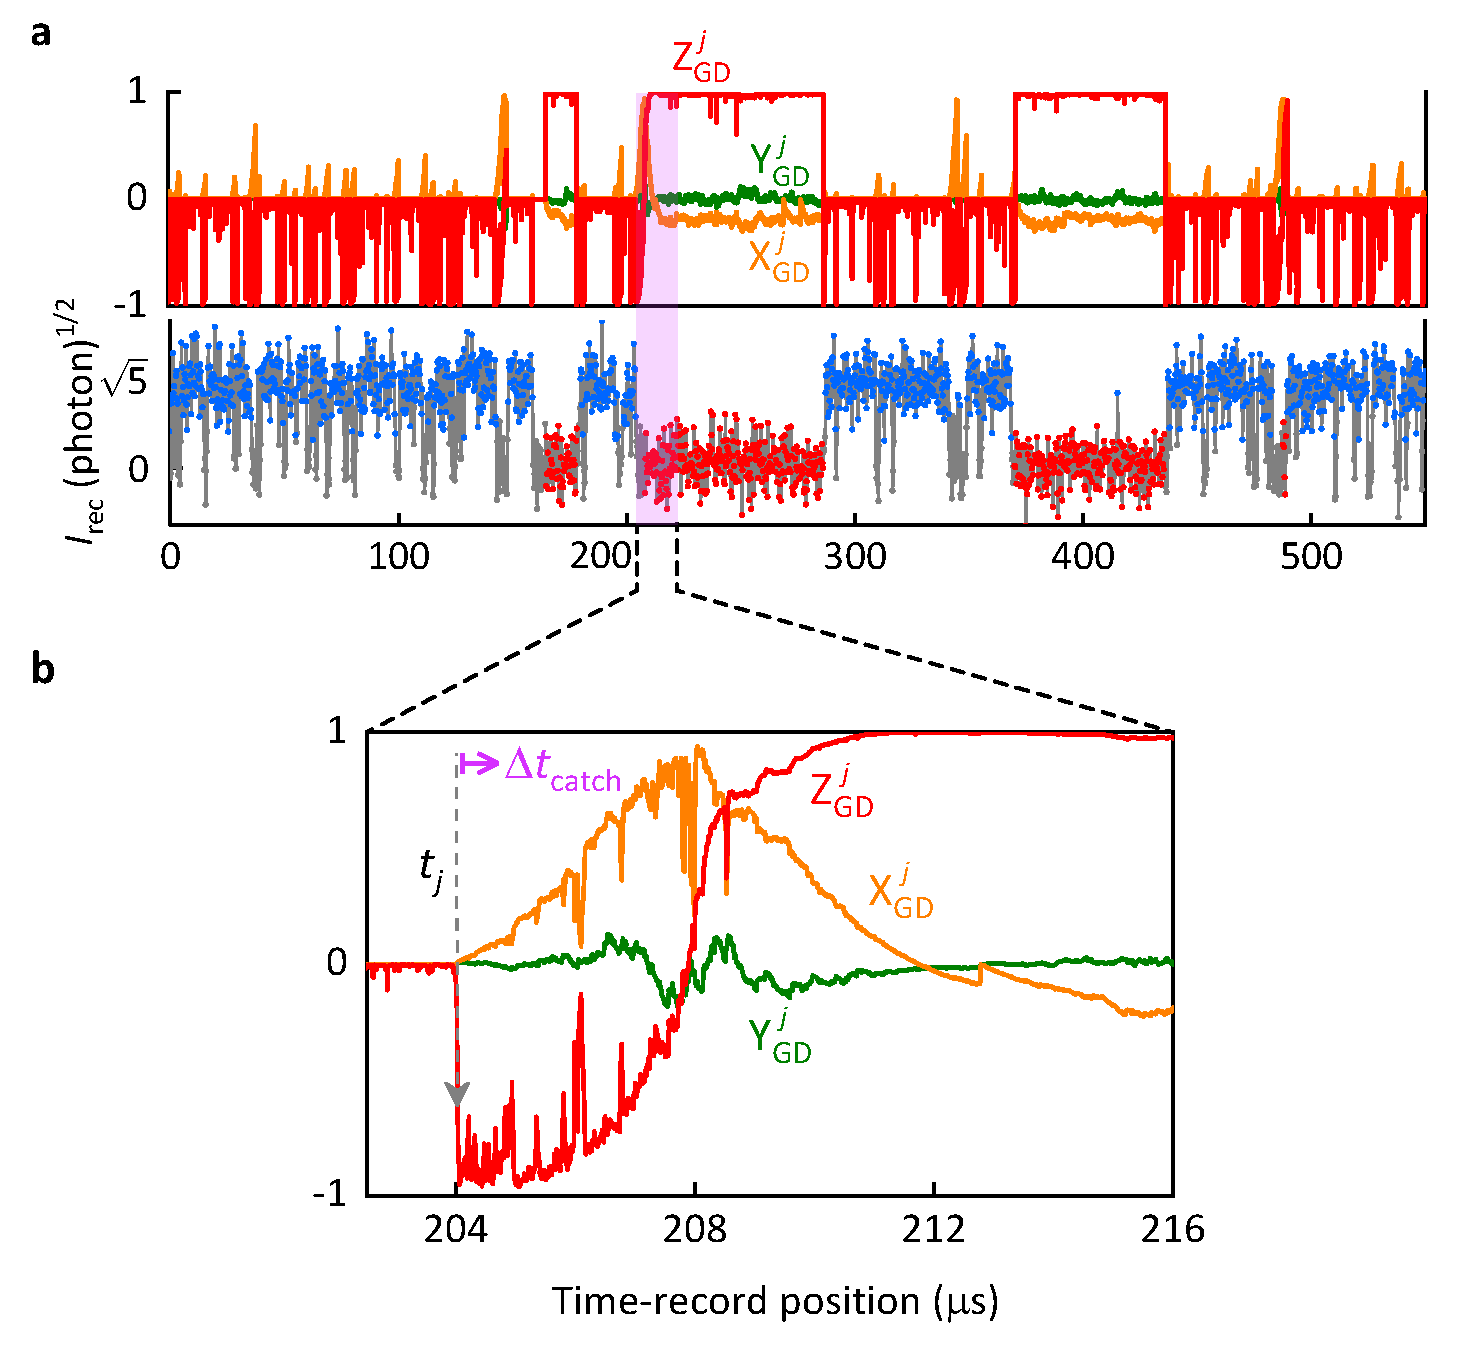
\includegraphics[width=145mm]{results/SamplingMC}\caption[Sampling of the Monte-Carlo simulation (courtesy of H.J. Carmichael)]{\label{fig:monte-carlo} \textbf{Sampling of the Monte-Carlo simulation.}
\textbf{a,} Simulated measurement quadrature $I_{{\rm rec}}$ and
correlated trajectory computed from Eqs.~(\ref{eqn:correlated_Z_GD})
and (\ref{eqn:correlated_X_GD=000026Y_GD}). Three sample intervals
are shown. The earliest corresponds to leakage from the GBD-manifold,
where a jump from $|{\rm G}\rangle$ to $|{\rm F}\rangle$ is followed
by a jump from $|{\rm F}\rangle$ to $|{\rm D}\rangle$. The second
and third sample intervals correspond to direct transitions from $|{\rm G}\rangle$
to $|{\rm D}\rangle$, which are continuously monitored and the object
of the experiment. \textbf{b,} Expanded view of the shaded region
of the second sample interval in panel (a). The evolution is continuous
but not smooth, due to backaction noise from the continuously monitored
readout. This feature is in sharp contrast to the perfect ``no-click''
readout upon which the simple theory of Sec.~\ref{sec:Fluorescence-monitored-by}
is based. Figure courtesy of H.J. Carmichael.}
\end{figure}

\begin{figure}
\centering{}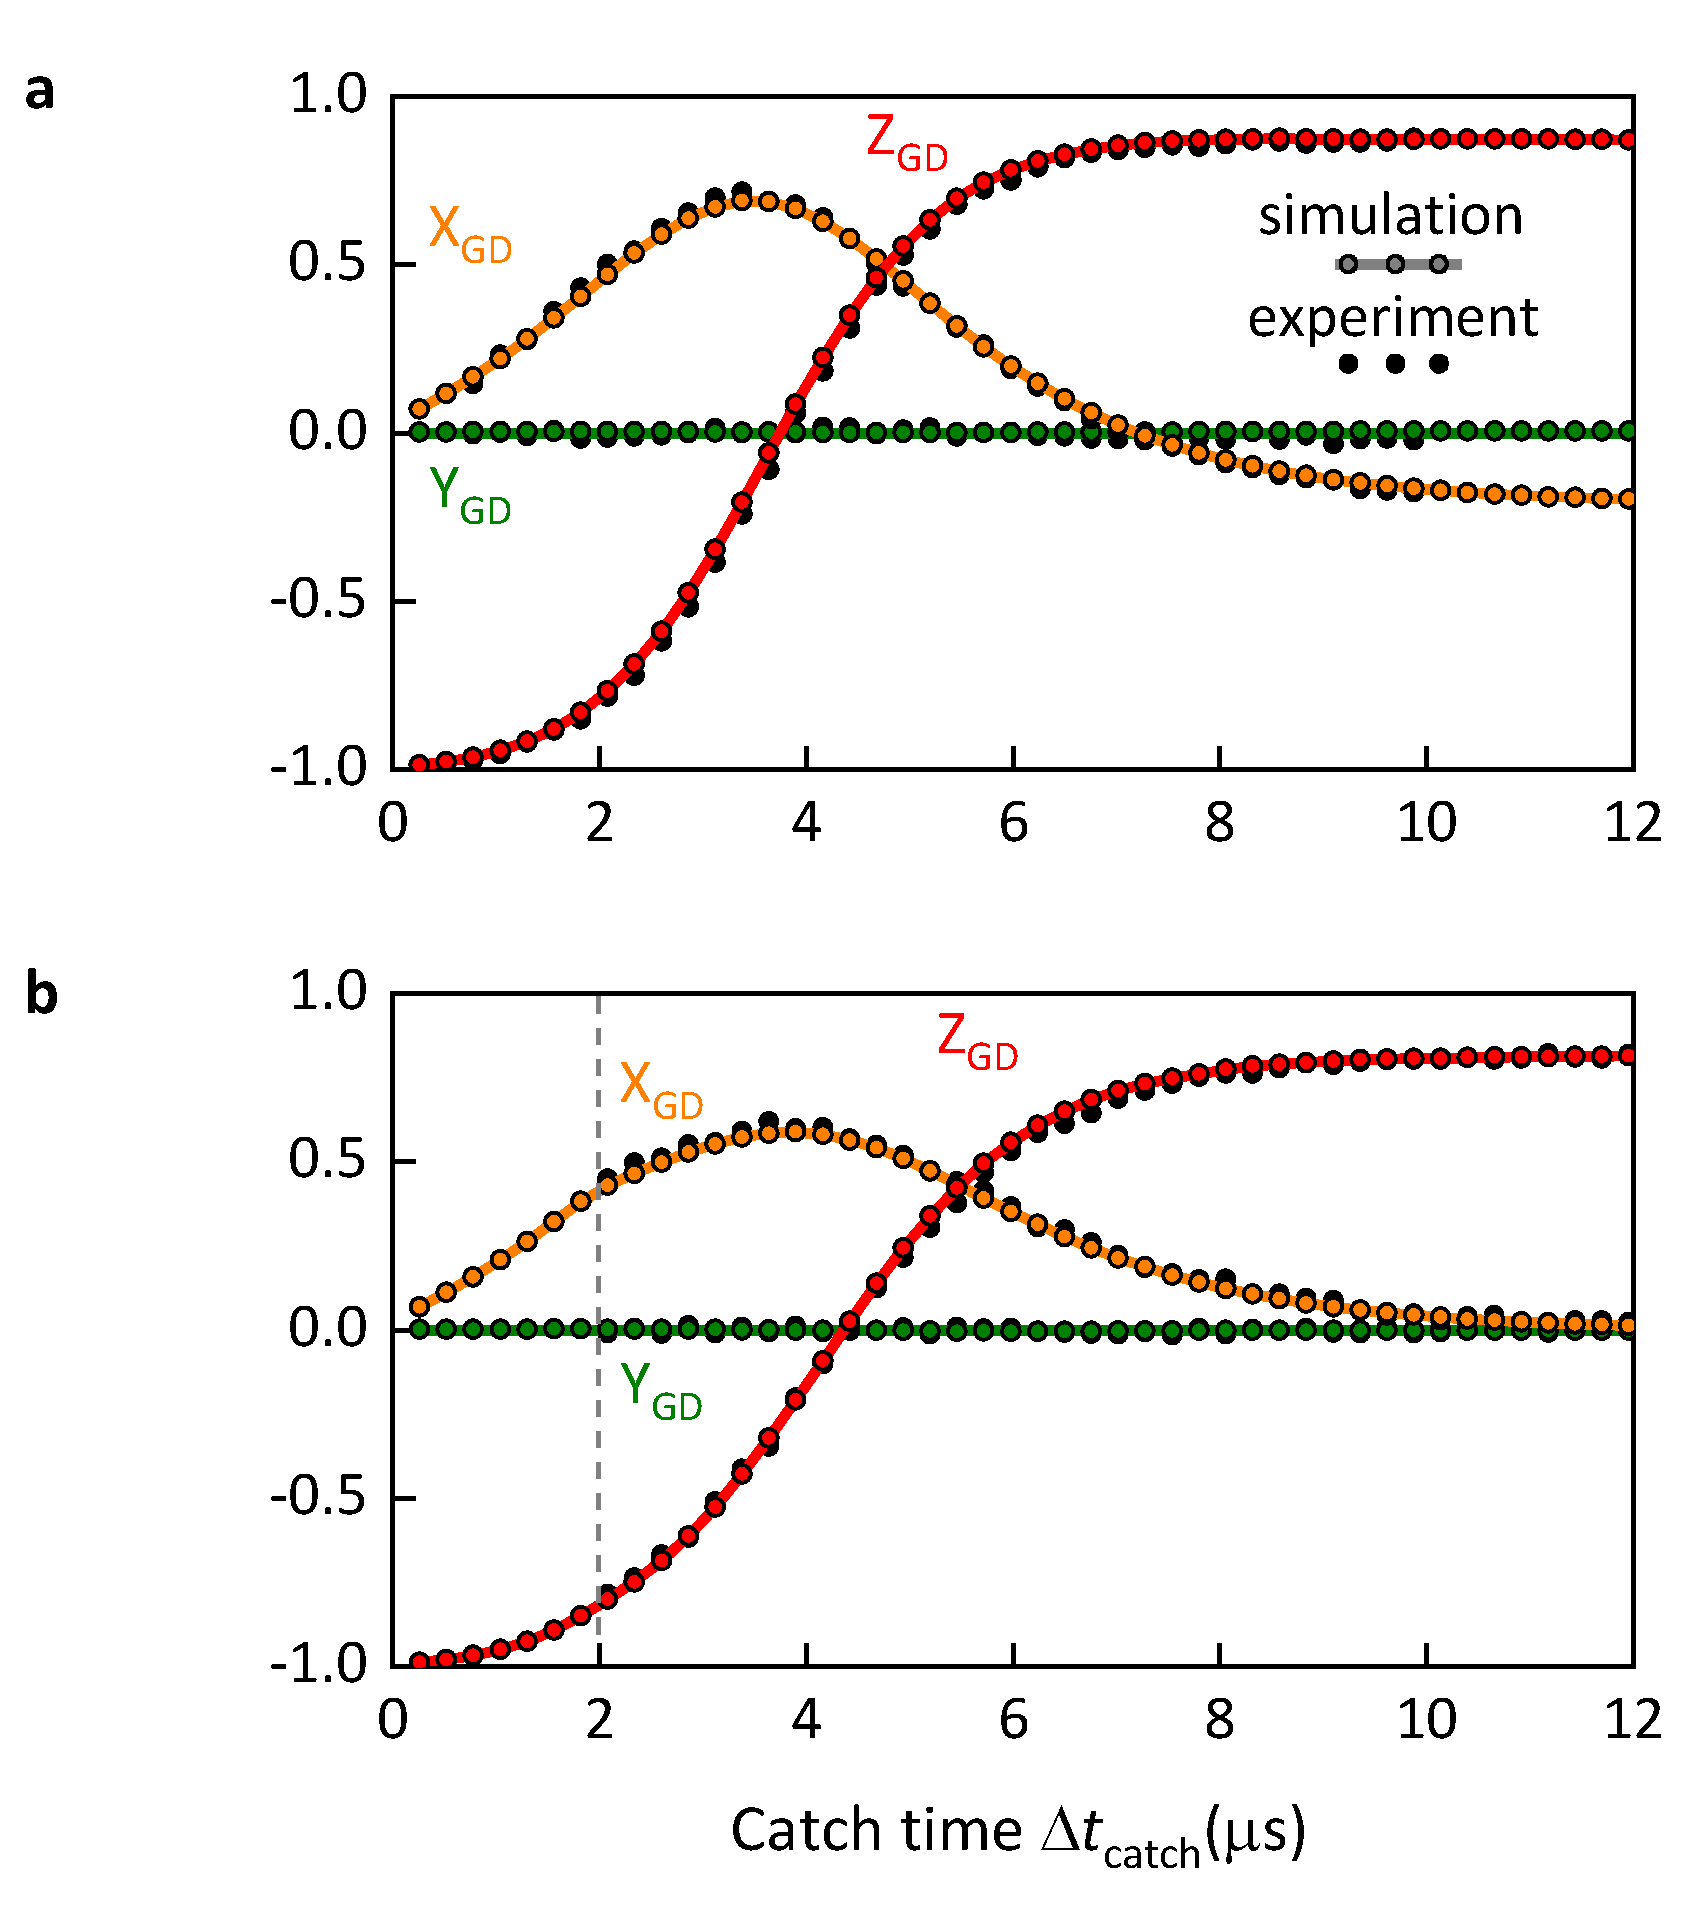
\includegraphics[width=120mm]{results/tomoCompar}\caption[Comparison between simulation and experiment (courtesy of H.J. Carmichael)]{\label{fig:simulation_vs_experiment} \textbf{Comparison between
simulation and experiment.} \textbf{a,} Simulated data set obtained
with Rabi drive $\Omega_{{\rm DG}}$ turned on for the entire $\Delta t_{{\rm catch}}$;
parameters taken from Table \ref{table:table2} and leakage from the
GBD-manifold included with $(\gamma_{{\rm FG}},\gamma_{{\rm FD}})/2\pi=0.38\mkern2mu {\rm kHz}$
and $(\gamma_{{\rm GF}},\gamma_{{\rm DF}})/2\pi=11.24\mkern2mu {\rm kHz}$.
\textbf{b,} Simulated data set obtained with Rabi drive $\Omega_{{\rm DG}}$
turned off at time $\Delta t_{{\rm on}}=2\mkern2mu \mu{\rm s}$; parameters
taken from Table \ref{table:table2} and leakage from the GBD-manifold
included with $\gamma_{{\rm FG}}/2\pi=0.217\mkern2mu {\rm kHz}$,
$\gamma_{{\rm FD}}/2\pi=4.34\mkern2mu {\rm kHz}$, $\gamma_{{\rm GF}}/2\pi=11.08\mkern2mu {\rm kHz}$,
and $\gamma_{{\rm DF}}/2\pi=15.88\mkern2mu {\rm kHz}$. When leakage
from the GBD-manifold is omitted, the ${\rm Z}_{{\rm GD}}$ curve
rises more sharply and settles to a value that is 10\% (20\%) higher
in panel (a) (panel (b)). Figure courtesy of H.J. Carmichael.}
\end{figure}

\clearpage{}

\begin{table}
\begin{centering}
\begin{tabular}{c}
\textbf{(a)} In presence of $\Omega_{\mathrm{DG}}$\tabularnewline
\tabularnewline
\centering{}\renewcommand*{\arraystretch}{1.2} %
\begin{tabular}{cc|crcllrrlcr}
Parameter  & \multicolumn{1}{c|}{} &  & \multicolumn{3}{c}{Experiment} &  & \multicolumn{3}{c}{Simulation} &  & Error\tabularnewline
\hline 
\rule{0pt}{3ex} $a$  &  &  & -0.07  & $\pm$  & 0.005  &  & -0.07  & $\pm$  & 0.005  &  & 0.5\%\tabularnewline
$a'$  &  &  & -0.21  & $\pm$  & 0.005  &  & -0.22  & $\pm$  & 0.005  &  & 2\%\tabularnewline
$b$  &  &  & 0.94  & $\pm$  & 0.005  &  & 0.95  & $\pm$  & 0.005  &  & 1\%\tabularnewline
$b'$  &  &  & 0.93  & $\pm$  & 0.005  &  & 0.91  & $\pm$  & 0.005  &  & 2\%\tabularnewline
$c$  &  &  & -2.32  & $\pm$  & 0.03  &  & -2.27  & $\pm$  & 0.03  &  & 2\%\tabularnewline
$c'$  &  &  & -2.04  & $\pm$  & 0.03  &  & -2.05  & $\pm$  & 0.03  &  & 0.5\%\tabularnewline
$\tau$  &  &  & 1.64  & $\pm$  & 0.01  &  & 1.65  & $\pm$  & 0.01  &  & 0.5\%\tabularnewline
$\tau'$  &  &  & 1.74  & $\pm$  & 0.01  &  & 1.76  & $\pm$  & 0.01  &  & 1\%\tabularnewline
\end{tabular}\tabularnewline
\tabularnewline
\textbf{(b)} In absence of $\Omega_{\mathrm{DG}}$\tabularnewline
\tabularnewline
\centering{}\renewcommand*{\arraystretch}{1.2} %
\begin{tabular}{cc|crcllrrlcr}
Parameter & \multicolumn{1}{c|}{} &  & \multicolumn{3}{c}{Experiment} &  & \multicolumn{3}{c}{Simulation} &  & Error\tabularnewline
\hline 
\rule{0pt}{3ex} $a$ &  &  & -0.11 & $\pm$ & 0.005 &  & -0.10 & $\pm$ & 0.005 &  & 8\%\tabularnewline
$a'$ &  &  & 0 & $\pm$ & 0 &  & 0 & $\pm$ & 0 &  & 0\%\tabularnewline
$b$ &  &  & 0.92 & $\pm$ & 0.008 &  & 0.91 & $\pm$ & 0.008 &  & 1\%\tabularnewline
$b'$ &  &  & 0.61 & $\pm$ & 0.005 &  & 0.60 & $\pm$ & 0.005 &  & 2\%\tabularnewline
$c$ &  &  & -1.96 & $\pm$ & 0.05 &  & -2.10 & $\pm$ & 0.05 &  & 7\%\tabularnewline
$c'$ &  &  & -1.97 & $\pm$ & 0.05 &  & -2.05 & $\pm$ & 0.05 &  & 4\%\tabularnewline
$\tau$ &  &  & 2.17 & $\pm$ & 0.05 &  & 2.03 & $\pm$ & 0.05 &  & 6\%\tabularnewline
$\tau'$ &  &  & 1.98 & $\pm$ & 0.05 &  & 1.92 & $\pm$ & 0.05 &  & 3\%\tabularnewline
\end{tabular}\tabularnewline
\tabularnewline
\end{tabular}
\par\end{centering}
\caption[Comparison between parameters extracted from the simulation and those
from the experiment. ]{\label{tab:Comparison-of-parameters} \textbf{Comparison between
parameters extracted from the simulation and those from the experiment}.
\textbf{a,} Parameters obtained from fits of the simulated and measured
data for the catch protocol in the presence of the Rabi drive $\Omega_{{\rm DG}}$
throughout the entire duration of the quantum jump, data shown in
Fig.~\ref{fig:simulation_vs_experiment}a. \textbf{b,} Parameters
obtained from fits of the simulated and measured data for the catch
protocol in the absence of the $\Omega_{{\rm DG}}$ during the flight
of the quantum jump for $\Delta t_{\mathrm{on}}=2\mathrm{\ \mu s}$,
data shown in Fig.~\ref{fig:simulation_vs_experiment}b. }
\end{table}

\clearpage{}

\subsection{Error budget\label{sec:Budget-coherence}}

In this section, we examine the effect of the various imperfections
and dissipation channels on the fidelity of the catch protocol. 

\paragraph{\textit{\emph{Imperfections.}}}

The various imperfections are expected to reduce the maximum coherence
recovered in the measurement of ${\rm X}_{{\rm GD}}(\Delta t_{{\rm catch}})$.
They include: 
\begin{enumerate}
\item Readout errors when inferring $|{\rm B}\rangle$ to not-$|{\rm B}\rangle$
transitions and the reverse. Such errors affect the assignment of
$\Delta t_{{\rm catch}}$, which can be either too short or too long
to correlate correctly with the true state of the system. 
\item Leaks from the GBD-manifold to higher excited states. Importantly,
these errors mimic a $|{\rm B}\rangle$ to not-$|{\rm B}\rangle$
transition, as in the first sample interval of Fig.~\ref{fig:monte-carlo},
but the anticipated coherent evolution within the GBD-manifold does
not occur. In this manner, the excitations to higher states lead to
false detections.
\item Thermal jumps from $|{\rm G}\rangle$ to $|{\rm D}\rangle$. Such
incoherent transitions contribute in a similar way to ${\rm Z}_{{\rm GD}}(\Delta t_{{\rm catch}})$,
while making no contribution to the measured coherence. 
\item Direct dephasing of the DG-coherence, $T_{\mathrm{2R}}^{\mathrm{D}}$. 
\item Partial distinguishability of $|{\rm G}\rangle$ and $|{\rm D}\rangle$.
The readout cavity is not entirely empty of photons when the state
is not-$|{\rm B}\rangle$, in which case the cross-Kerr interaction
$\chi_{{\rm D}}|{\rm D}\rangle\langle{\rm D}|\hat{c}^{\dagger}\hat{c}$
shifts the $\Omega_{{\rm DG}}$ Rabi drive from resonance; hence,
backaction noise is transferred from the photon number to ${\rm X_{{\rm GD}}}(\Delta t_{{\rm catch}})$. 
\end{enumerate}

\paragraph{\textit{\emph{Budget for lost coherence.}}\emph{ }}

The maximum coherence reported in the experiment is $0.71\pm0.005$.
In the simulation it is a little lower at 0.69. By removing the imperfections
from the simulation, one by one, we can assign a fraction of the total
coherence loss to each. Readout errors are eliminated by identifying
transitions between $|{\rm B}\rangle$ and not-$|{\rm B}\rangle$
in the ket $|\psi\rangle$ rather than from the simulated measurement
record; all other imperfections are turned off by setting some parameter
to zero. The largest coherence loss comes from readout errors, whose
elimination raises the ${\rm X}_{{\rm GD}}(\Delta t_{{\rm catch}})$
maximum by 0.09. The next largest comes from leakage to higher excited
states, which raises the maximum by a further 0.06. Setting $\chi_{{\rm D}}$
to zero adds a further 0.04, and thermal transitions and pure dephasing
together add 0.02. Figure~\ref{fig:coherence_loss} illustrates the
change in the distribution of ${\rm X}_{{\rm GD}}^{j}(\Delta t_{{\rm catch}})$
samples underlying the recovery of coherence. The removal of the finger
pointing to the left in panel (a) is mainly brought about by the elimination
of readout errors, while the reduced line of zero coherence marks
the elimination of leakage to higher excited states. Aside from these
two largest changes, there is also a sharpening of the distribution,
at a given $\Delta t_{{\rm catch}}$, when moving from panel (a) to
panel (b). Having addressed the five listed imperfections, a further
10\% loss remains unaccounted for, i.e., the distribution of panel
(b) is not a line passing through ${\rm X}_{{\rm GD}}^{j}(\Delta t_{{\rm mid}})=1$.
The final 10\% is explained by the heterodyne detection backaction
noise, a function of the drive and measurement parameters, displayed
in panel (b) of Fig.~\ref{fig:monte-carlo}. 
\begin{figure}[h]
\begin{centering}
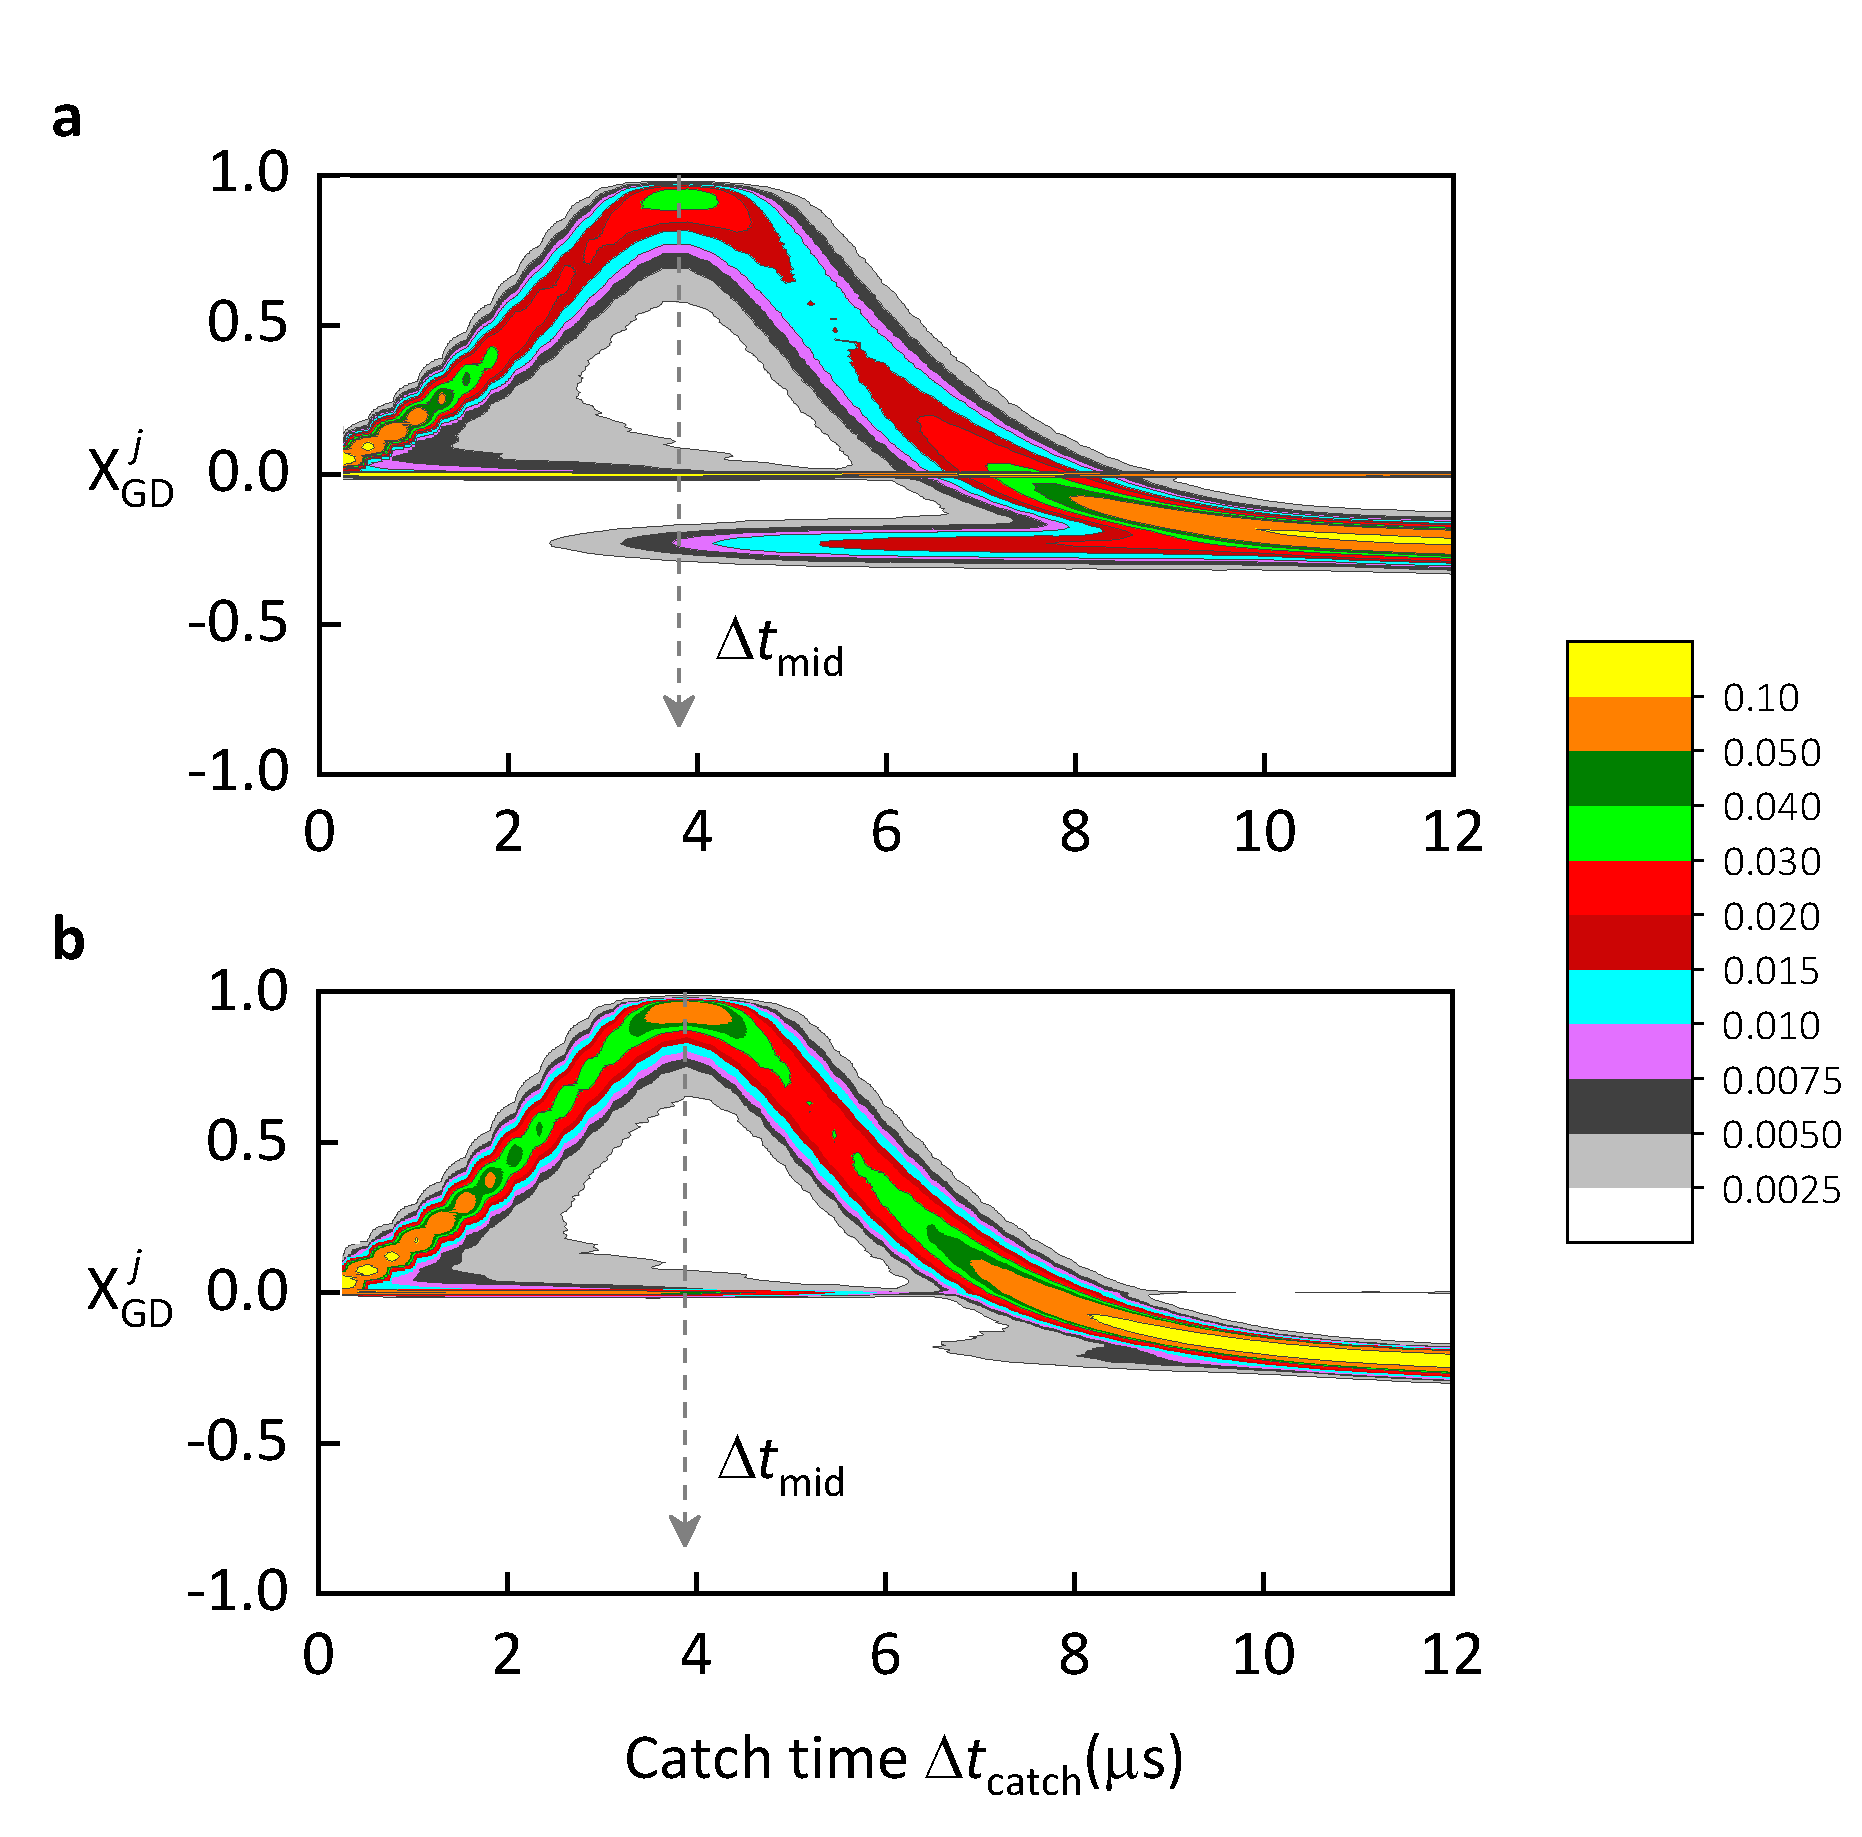
\includegraphics[width=130mm]{results/traj_hist}
\par\end{centering}
\centering{}\caption[Coherence loss through sample to sample fluctuations (courtesy of
H.J. Carmichael)]{\label{fig:coherence_loss}\textbf{Coherence loss through sample
to sample fluctuations.} \textbf{a,} Contour plot of the distribution
of ${\rm X}_{{\rm GD}}^{j}(\Delta t_{{\rm catch}})$ samples corresponding
to the simulated data set displayed in panel (a) of Fig.~\ref{fig:simulation_vs_experiment}.
\textbf{b,} Same as panel (a) but with transitions between $|{\rm B}\rangle$
and not-$|{\rm B}\rangle$ identified in the ket $|\psi\rangle$ rather
than from the simulated measurement record, and with changed parameters:
$(\gamma_{{\rm FG}},\gamma_{{\rm FD}},\gamma_{{\rm GF}},\gamma_{{\rm DF}})/2\pi=0$,
$n_{{\rm th}}^{{\rm B}}=n_{{\rm th}}^{{\rm D}}=0$, $T_{2}^{{\rm D}}=2T_{1}^{{\rm D}}$,
and $\chi_{{\rm D}}/2\pi=0$. Figure courtesy of H.J. Carmichael.}
\end{figure}


\section{Signal-to-noise ratio (SNR) and de-excitation measurement efficiency\label{subsec:Signal-to-noise-ratio-(SNR)}}

The catch protocol hinges on the efficient detection of de-excitations
from $|{\rm B}\rangle$ to $|{\rm G}\rangle$, as discussed in more
detail in Chapter~\ref{chap:theoretical-description-jumps}. In atomic
physics, de-excitations are typically monitored by a \emph{direct}
detection method, employing a photodetector. Alternatively, de-excitations
can be monitored by an\emph{ indirect} method, as done in our experiment.
In this section, we discuss the efficiency of both methods. For the
indirect method, using simple analytics, we estimate the \emph{total}
efficiency of time-continuous, uninterrupted monitoring of de-excitations
from $|{\rm B}\rangle$ to $|{\rm G}\rangle$ to be $\eta_{\mathrm{eff,clk}}=0.90\pm0.01$
for the parameters of our experiment, with integration time $T_{\mathrm{int}}=0.26\,\mathrm{\mu s}$.
The simple analysis of this section complements the numerical one
of the previous section, Sec.~\ref{sec:Budget-coherence}.

\emph{Direct monitoring method in atomic physics.} The direct method
monitors for a $|{\rm B}\rangle$ de-excitation by collecting and
absorbing the photon radiated in the de-excitation. The \emph{total}
measurement efficiency of this method is limited by i) collection
efficiency --- the fraction of emitted photons collected by the detector
in its own input spatial modes (for instance, as determined by the
solid angle) --- typically falls in the range 0.1 - 50\%, \citep{Volz2011}
ii) the efficiency of detecting the absorption of a single photon,
which falls in the range 1 - 90\%, \citep{Eisaman2011} and iii) non-idealities
of the photodetector apparatus, including its dead time, dark counts,
jitter, etc. \citep{Eisaman2011} The combination of these inefficiencies
presents an almost insurmountable challenge in experimental atomic
physics for realizing continuous, time-resolved detection of nearly
every single photon emitted by the three-level atom, required to faithfully
catch the jump. 

\emph{Direct monitoring method with superconducting circuits.} While
technologically very different, the direct monitoring method with
superconducting circuits is conceptually similar to atomic method
but can readily achieve high collection efficiencies \citep{Katz2008,Vijay2011,Riste2012-qubit-measure-reset,Vijay2012,Hatridge2013,Murch2013a,deLange2014,Roch2014,Weber2014,Campagne-Ibarcq2014,Macklin2015,Campagne2016-Fluorescence,Campagne-Ibarcq2016,Hacohen-Gourgy2016-non-comm,Naghiloo2016,White2016,Ficheux2017,Naghiloo2017-thermo,Tan2017,Hacohen-Gourgy2018,Heinsoo2018,Bultink2018}.
 However, the energy of the emitted microwave photon is exceedingly
small --- $23\text{ }\mathrm{\mu eV}$, about a part per 100,000
of the energy of a single optical photon --- which essentially forbids
the direct detection of the photon with near-unit efficiency. This
is because the propagating photon is unavoidably subjected to significant
loss, added spurious noise, amplifier non-idealities, etc. In our
experiment, these imperfections reduce the full measurement/amplification
chain efficiency from its ideal value \citep{Hatridge2013,Macklin2015,Bultink2018}
of 1 to a modest $\eta=0.33\pm0.03$, corresponding to the direct
detection of approximately only one out of every three single photons
--- insufficient for the catch protocol.

\subsubsection{Indirect monitoring method with superconducting circuits}

Alternatively, the indirect monitoring method couples the atom to
an ancillary degree of freedom, which is itself monitored in place
of the atom. In our experiment, the atom is strongly, dispersively
coupled to the ancillary readout cavity. The cavity scatters a probe
tone, whose phase shift constitutes the readout signal, as discussed
in Chapter~\ref{chap:theoretical-description-jumps}. Since the probe
tone can carry itself many photons, this scheme increases the signal-to-noise
ratio ($\mathrm{SNR}$) and, hence, the total efficiency ($\eta_{\mathrm{eff,clk}}$)
of detecting a $|{\rm B}\rangle$ de-excitation. Note that the efficiency
$\eta_{\mathrm{eff,clk}}$ should not be confused with the efficiency
of a photodetector or the efficiency $\eta$ of the measurement/amplification
chain, since $\eta_{\mathrm{eff,clk}}$ includes the effect of all
readout imperfections and non-idealities, state discrimination and
assignment errors, etc. see below. In the remainder of this section,
we estimate the SNR and efficiency $\eta_{\mathrm{eff,clk}}$ of the
experiment.

\emph{SNR of the indirect (dispersive) method.}  The output of the
measurement and amplification chain monitoring the readout cavity
is proportional to the complex heterodyne measurement record $\zeta\left(t\right)$,
which obeys the It\^{o} stochastic differential equation, see Eq.~(\ref{eq:Record}),\footnote{Since the bandwidth of the measurement chain, $\kappa_{\mathrm{filter}}$,
is significantly larger than that, $\kappa$, of the readout cavity,
$\kappa_{\mathrm{filter}}\gg\kappa$, we can neglect the effect of
$\kappa_{\mathrm{filter}}$ for simplicity of discussion, see Eqs.~(\ref{eqn:simulated_I_int})
and~(\ref{eqn:simulated_Q_int}).} 
\begin{equation}
\mathrm{d}\zeta\left(t\right)=\sqrt{\eta\kappa}\frac{\langle\psi\left(t\right)|\hat{a}|\psi\left(t\right)\rangle}{\langle\psi\left(t\right)|\psi\left(t\right)\rangle}\mathrm{d}t+\mathrm{d}Z\left(t\right),\label{eq:heterodyne-current2}
\end{equation}
where $\hat{a}$ is the cavity amplitude operator in the Schr\"{o}dinger
picture, $\eta$ is the total measurement efficiency of the amplification
chain --- again, not to be confused with the de-excitation measurement
efficiency, $\eta_{\mathrm{eff,clk}}$ --- and $\mathrm{d}Z$ is
the complex Wiener process increment, defined below Eq.~(\ref{eq:heterodyne-current2}).
A somewhat counterintuitive property of Eq.~(\ref{eq:heterodyne-current2})
is that  the heterodyne record increment $\mathrm{d}\zeta\left(t\right)$
is stochastic and noisy even when $\eta=1$, the case of ideal measurement
in which no signal is lost --- the stochastic term, $\mathrm{d}Z$,
represents pure quantum vacuum fluctuations, which are inherent in
the case of heterodyne detection \citep{Carmichael1993,Plenio1998,wiseman2010book}.
Due to the unavoidable presence of these fluctuations, only an infinitesimal
amount of information about the system can be extracted from $\mathrm{d}\zeta$
at an instant of time. Finite amount of information is extracted by
integrating $\mathrm{d}\zeta$ for a finite duration $T_{\mathrm{int}}$,
\begin{equation}
s\equiv I_{\mathrm{rec}}+iQ_{\mathrm{rec}}\equiv\int_{0}^{T_{\mathrm{int}}}\mathrm{d}\zeta\left(t\right)\,,\label{eq:s=00003D}
\end{equation}
where $I_{\mathrm{rec}}$ and $Q_{\mathrm{rec}}$ are the in- and
out-of-phase quadrature components of one segment of the record. What
does $s$ correspond to? Its value depends on $\mathrm{d}\zeta$,
which depends on the state of the cavity, $|\psi\rangle$, which itself
depends on the occupation of $\ket{\mathrm{B}}$ --- and therefore
$s$ contains the occupation of $\ket{\mathrm{B}}$. A de-excitation
of $\ket{\mathrm{B}}$ to $\ket{\mathrm{G}}$ can thus be detected
by monitoring $s$, whose value is different for the two states, since
the cavity is generally in the coherent state $\ket{\alpha_{\mathrm{B}}}$
or $\ket{\alpha_{\mathrm{G}}}$ when the atom is in $\ket{\mathrm{B}}$
or $\ket{\mathrm{G}}$, respectively. For the moment, assuming the
atom and cavity do not change states during the course of the measurement
duration $T_{\mathrm{int}}$, the stochastic integral in Eq.~(\ref{eq:s=00003D})
explicitly evaluates to 
\begin{equation}
s_{\mathrm{B,G}}=\left\{ \sqrt{\eta\kappa}\mathrm{Re}\left[\alpha_{\mathrm{B,G}}\right]T_{\mathrm{int}}+\frac{1}{\sqrt{2}}W_{I}\left(T_{\mathrm{int}}\right)\right\} +i\left\{ -\sqrt{\eta\kappa}\mathrm{Im}\left[\alpha_{\mathrm{B,G}}\right]T_{\mathrm{int}}+\frac{1}{\sqrt{2}}W_{Q}\left(T_{\mathrm{int}}\right)\right\} \,,\label{eq:s=00003DExplicit}
\end{equation}
where $W_{I,Q}$ denote independent Wiener processes, obeying the
conventional rules, $\mathrm{E}\left[W\left(t\right)\right]=0$ and
$\mathrm{Var}\left[W\left(t\right)\right]=t^{2}$. Equation~(\ref{eq:s=00003DExplicit})
shows that the distribution of the stochastic variable $s$ is a Gaussian
blob in the IQ plane centered at $\bar{s}_{\mathrm{B,G}}\equiv\operatorname{E}\left[s_{\mathrm{B,G}}\right]=\sqrt{\eta\gamma}T_{\mathrm{int}}\alpha_{\mathrm{B,G}}$
with width determined by the variance $\sigma_{\mathrm{B,G}}^{2}\equiv\operatorname{Var}\left[s_{\mathrm{B,G}}\right]=\frac{1}{2}T_{\mathrm{int}}$.
We can thus define the SNR of the experiment by comparing the distance
between the two pointer distributions to their width, 
\begin{equation}
\mathrm{SNR}\equiv\left|\frac{\bar{s}_{\mathrm{B}}-\bar{s}_{\mathrm{G}}}{\sigma_{\mathrm{B}}+\sigma_{\mathrm{G}}}\right|^{2}\,,\label{eq:SNR-defn}
\end{equation}
where the B (resp., G) subscript denotes signals conditioned on the
atom being in $\ket{\mathrm{B}}$ (resp., $\ket{\mathrm{G}}$). In
terms of $\ket{\alpha_{\mathrm{B}}}$ and $\ket{\alpha_{\mathrm{G}}}$,
\begin{equation}
\mathrm{SNR}=\frac{1}{2}\eta\kappa T_{\mathrm{int}}\left|\alpha_{\mathrm{B}}-\alpha_{\mathrm{G}}\right|^{2}\,,
\end{equation}
which can be expressed in terms of the parameters of the experiment,
summarized in Table~\ref{tab:system-params},
\begin{equation}
\mathrm{SNR}=\frac{1}{2}\eta\kappa T_{\mathrm{int}}\left[\cos\left(\arctan\left(\frac{\kappa}{2\chi_{\mathrm{BG}}}\right)\right)\right]^{2}\bar{n}\,,\label{eq:SNR-expression}
\end{equation}
Holding other parameters fixed, according to Eq.~(\ref{eq:SNR-expression}),
the SNR can be increased arbitrarily by increasing $\bar{n}$, which
can be readily done by increasing the amplitude of the cavity probe
tone. A higher SNR for $s$ corresponds to a higher SNR for measuring
an atom de-excitation, since $s$ is a proxy of the $\ket{\mathrm{B}}$
population. Thus, the indirect cavity monitoring can overcome the
typical degradation in SNR imposed by the inefficiencies and non-idealities
of the measurement chain, $\eta$. In practice, the SNR increase
with $\bar{n}$ is bounded from above, since with sufficiently high
$\bar{n}$ spurious non-linear effects become significant \citep{Boissonneault2008,Boissonneault2009-Photon-induced-relax,Minev2013,Sank2016-T1vsNbar,Khezri2016,Bultink2016,Khezri2017,Walter2017,Lescanne2018,Verney2018,Serniak2018}.
The cavity and non-linear coupling to the atom serve in effect as
a rudimentary embedded pre-amplifier at the site of the atom, which
transduces with amplification the de-excitation signal before its
SNR is degraded during propagation and further processing.

\emph{Discrimination efficiency of the indirect method.} While the
SNR provides a basic characterization of the measurement, it is useful
to convert it to a number between 0 and 1, which is called the discrimination
efficiency, $\eta_{\mathrm{disc}}$. It quantifies the degree to which
the two Gaussian distributions of $s$ are distinguishable \citep{Gambetta2007-ProtocolsMsr},
\begin{equation}
\eta_{\mathrm{disc}}=\frac{1}{2}\operatorname{erfc}\left[-\sqrt{\frac{\mathrm{SNR}}{2}}\right]\,,\label{eq:eta-msr}
\end{equation}
where $\operatorname{erfc}$ denotes the complementary error function.
Equation~(\ref{eq:eta-msr}) shows that increasing the SNR by separating
the $s_{\mathrm{B}}$ and $s_{\mathrm{G}}$ distributions far beyond
their spread, $\sigma_{\mathrm{B/G}}$, provides only marginal gain
as $\eta_{\mathrm{disc}}$ saturates to 1. Next, we calculate the
SNR and $\eta_{\mathrm{disc}}$ for the parameters of the experiment
and discuss corrections due to readout non-idealities. 

\emph{A first comparison to the experiment. }A first estimate of the
SNR and $\eta_{\mathrm{disc}}$ of the experiment are provided by
Eqs.~(\ref{eq:SNR-expression}) and~(\ref{eq:eta-msr}). Using the
parameters of the experiment, summarized in Table~\ref{tab:system-params},
from these two equations, we find $\mathrm{SNR}=4.3\pm0.6$ and $\eta_{\mathrm{disc}}=0.98\pm0.007$.
Using data from the experiment, in particular, a second long IQ record
trace, represented by a short segment in Fig.~2a, we find the SNR
of the jumps experiment, by fitting the histogram of the trace with
a bi-Gaussian distribution, to be $\mathrm{SNR}=3.8\pm0.4$, corresponding
to $\eta_{\mathrm{\mathrm{disc}}}=0.96\pm0.01$. The measured values
are slightly lower than the analytics predict due to readout imperfections
not included in the calculation so far, such as state transitions
during $T_{\mathrm{int}}$, cavity transient dynamics, additional
pointer-state distributions, etc.

\emph{Effective click detection efficiency. }The dominant next-order
error is due to atom state transitions during the measurement window,
$T_{\mathrm{int}}$, which contributes an assignment error of approximately
$1-\eta_{\mathrm{asg}}=1-\exp\left(T_{\mathrm{int}}/\tau_{\mathrm{B}}\right)=0.06\pm0.001$
to the detection of a $|\mathrm{B}\rangle$ de-excitation. Combining
$\eta_{\mathrm{disc}}$ with $\eta_{\mathrm{asg}}$, we obtain the
total efficiency for detecting $\ket{\mathrm{B}}$ de-excitations
$\eta_{\mathrm{eff,clk}}=\eta_{\mathrm{disc}}\eta_{\mathrm{asg}}=0.90\pm0.01$,
consistent with the total readout efficiency of $0.91$ that is independently
estimated using the trajectory numerics, see Sec.~\ref{sec:Budget-coherence}.


\section{Directions and Conclusions}
\label{sec:conclusions}

We have presented our initial exploration of \DV\ across a wide range of tasks and domains, providing supporting evidence to the claim that \DV's abilities are comparable to human-level for many of them. This conclusion is consistent with the findings by OpenAI presented in \cite{gpt4}. A primary goal of our experiments is to give a preliminary assessment of \DV's {\em intelligence}, which is an arduous task given the lack of formal definition for this concept, especially for artificial systems. We hope that our exploration provides a useful and necessary first step to appreciate the remarkable capabilities and challenges of {\DV}, and that it opens up new opportunities for developing more formal and comprehensive methods for testing and analyzing future AI systems with such broad intelligence. The capabilities of the model, which have been demonstrated above, both in terms of depth and generality, suggest that the machine learning community needs to move beyond classical benchmarking via structured datasets and tasks, and that the evaluation of the capabilities and cognitive abilities of those new models have become much closer in essence to the task of evaluating those of a human rather than those of a narrow AI model. We hope our investigation stimulates further research on {\DV} and similar systems, both in terms of exploring new applications and domains, and in terms of understanding the mechanisms and principles that underlie their intelligence.
\newline

The central claim of our work is that \DV\ attains a form of \emph{general} intelligence, indeed showing {\em sparks of artificial general intelligence}. This is demonstrated by its core mental capabilities (such as reasoning, creativity, and deduction), its range of topics on which it has gained expertise (such as literature, medicine, and coding), and the variety of tasks it is able to perform (e.g., playing games, using tools, explaining itself, ...). A lot remains to be done to create a system that could qualify as a complete AGI. We conclude this paper by discussing several immediate next steps, regarding defining AGI itself, building some of missing components in LLMs for AGI, as well as gaining better understanding into the origin of the intelligence displayed by the recent LLMs.

\subsection{Definitions of intelligence, AI, and AGI} \label{sec:otherdefinitions}
In this paper, we have used the 1994 definition of intelligence by a group of psychologists \cite{gottfredson1997mainstream} as a guiding framework to explore \DV's artificial intelligence. This definition captures some important aspects of intelligence, such as reasoning, problem-solving, and abstraction, but it is also vague and incomplete. It does not specify how to measure or compare these abilities. Moreover, it may not reflect the specific challenges and opportunities of artificial systems, which may have different goals and constraints than natural ones. Therefore, we acknowledge that this definition is not the final word on intelligence, but rather a useful starting point for our investigation. There is a rich and ongoing literature that attempts to propose more formal and comprehensive definitions of intelligence, artificial intelligence, and artificial general intelligence \cite{goertzel2014artificial, chollet2019measure}, but none of them is without problems or controversies.
For instance, Legg and Hutter \cite{legg2008machine} propose a goal-oriented definition of artificial general intelligence: Intelligence measures an agent’s ability to achieve goals in a wide range of environments. However, this definition does not necessarily capture the full spectrum of intelligence, as it excludes passive or reactive systems that can perform complex tasks or answer questions without any intrinsic motivation or goal. One could imagine as an artificial general intelligence, a brilliant oracle, for example, that has no agency or preferences, but can provide accurate and useful information on any topic or domain. Moreover, the definition around achieving goals in a wide range of environments also implies a certain degree of universality or optimality, which may not be realistic (certainly human intelligence is in no way universal or optimal). The need to recognize the importance of priors (as opposed to {\em universality}) was emphasized in the definition put forward by Chollet in \cite{chollet2019measure} which centers intelligence around skill-acquisition efficiency, or in other words puts the emphasis on a single component of the 1994 definition: learning from experience (which also happens to be one of the key weaknesses of LLMs). Another candidate definition of artificial general intelligence from Legg and Hutter \cite{legg2007universal} is: a system that can do anything a human can do. However, this definition is also problematic, as it assumes that there is a single standard or measure of human intelligence or ability, which is clearly not the case. Humans have different skills, talents, preferences, and limitations, and there is no human that can do everything that any other human can do. Furthermore, this definition also implies a certain anthropocentric bias, which may not be appropriate or relevant for artificial systems. While we do not adopt any of those definitions in the paper, we recognize that they provide important angles on intelligence. For example, whether intelligence can be achieved without any agency or intrinsic motivation is an important philosophical question. Equipping LLMs with agency and intrinsic motivation is a fascinating and important direction for future work. With this direction of work, great care would have to be taken on alignment and safety per a system's abilities to take autonomous actions in the world and to perform autonomous self-improvement via cycles of learning. We discuss a few other crucial missing components of LLMs next.

\subsection{On the path to more general artificial intelligence}
%We have provided evidence supporting that claim that {\DV} performance on a wide range of tasks is comparable to human-level abilities. We have argued that the model attains a form of \emph{general} intelligence in terms of core mental capabilities (such as reasoning, creativity, and deduction), in terms of the range of topics on which is has gained expertise (such as literature, medicine, and coding), and in terms of the variety of tasks it is able to perform (e.g., playing games, using tools, explaining itself, ...). We have also shown that {\DV} can generate and understand content that combines different topics, skills, and modalities, demonstrating its flexibility and creativity and that, despite being trained purely on text, it demonstrates remarkable capabilities in a variety of modalities such as vision. We have compared {\DV}'s performance to those of previous large language models (LLMs), most notably ChatGPT \cite{gpt3}, and we have found that {\DV} is far superior in terms of generality, creativity, and closeness to human-level intelligence. 

%As we allude to in the title of the paper, this work explores a ``first contact" with {\DV} and its potential descendants, rather than a comprehensive evaluation of the model's intelligence. We hope that our exploration provides a useful and necessary first step to appreciate the remarkable capabilities and challenges of {\DV}, and that it opens up new opportunities for developing more formal and comprehensive methods for testing and analyzing future AGI systems. The capabilities of the model, which have been demonstrated above, both in terms of depth and generality, suggest that the machine learning community needs to move beyond classical benchmarking via structured datasets and tasks, and that the evaluation of the capabilities and cognitive abilities of those new models have become much closer in essence to the task of evaluating those of a human rather than those of a narrow AI model. We hope our investigation stimulates further research on {\DV} and similar systems, both in terms of exploring new applications and domains, and in terms of understanding the mechanisms and principles that underlie their intelligence.

%We have also identified some of the main drawbacks of \DV, and we have discussed how they might be addressed in future work. These drawbacks include:
Some of the areas where \DV\ (and LLMs more generally) should be improved to achieve more general intelligence include (note that many of them are interconnected):
\begin{itemize}
    \item \textbf{Confidence calibration:} The model has trouble knowing when it should be confident and when it is just guessing. It both makes up facts that have not appeared in its training data, and also exhibits inconsistencies between the generated content and the prompt, which we referred to as {\em open-domain} and {\em closed-domain} hallucination in Figure \ref{fig:hallucination}. These hallucinations can be stated in a confident and persuasive manner that can be difficult to detect. Thus, such generations can lead to errors, and also to confusion and mistrust. While hallucination is a good thing when generating creative content, reliance on factual claims made by a model with hallucinations can be costly, especially for uses in high-stakes domains such as healthcare. There are several complementary ways to attempt to address hallucinations. One way is to improve the calibration of the model (either via prompting or fine-tuning) so that it either abstains from answering when it is unlikely to be correct or provides some other indicator of confidence that can be used downstream. Another approach, that is suitable for mitigating open-domain hallucination, is to insert information that the model lacks into the prompt, for example by allowing the model to make calls to external sources of information, such as a search engine as in Section \ref{sec:affordances}. For closed-domain hallucination the use of additional model computation through post-hoc checks is also promising, see Figure \ref{fig:hallucination} for an example. Finally, building the user experience of an application with the possibility of hallucinations in mind can also be part of an effective mitigation strategy. %Other directions include developing and refining mechanisms that endow systems with well-calibrated likelihoods that its generations are grounded, or, more directly, the likelihood that it is hallucinating versus relying upon and communicating content that it has learned from its training data. 
    \item \textbf{Long-term memory:} The model's context is very limited (currently 8000 tokens, but not scalable in terms of computation), it operates in a ``stateless" fashion and there is no obvious way to teach the model new facts. In fact, it is not even clear whether the model is able to perform tasks which require an evolving memory and context, such as reading a book, with the task of following the plot and understanding references to prior chapters over the course of reading.
    \item \textbf{Continual learning:} The model lacks the ability to update itself or adapt to a changing environment. The model is fixed once it is trained, and there is no mechanism for incorporating new information or feedback from the user or the world. One can fine-tune the model on new data, but this can cause degradation of performance or overfitting. Given the potential lag between cycles of training, the system will often be out of date when it comes to events, information, and knowledge that came into being after the latest cycle of training.
    \item \textbf{Personalization:} Some of the applications require the model to be tailored to a specific organization or end user. The system may need to acquire knowledge about the workings of an organization or the preferences of an individual. And in many cases, the system would need to adapt in a personalized manner over periods of time with specific changes linked to the dynamics of people and organizations. For example, in an educational setting, there would be an expectation of the need for the system to understand particular learning styles as well as to adapt over time to a student's progress with comprehension and prowess. The model does not have any way to incorporate such personalized information into its responses, except by using meta-prompts, which are both limited and inefficient. 
    \item \textbf{Planning and conceptual leaps:} As suggested by the examples in Section \ref{sec:limitations}, the model exhibits difficulties in performing tasks that require planning ahead or that require a ``Eureka idea" constituting a discontinuous conceptual leap in the progress towards completing a task. In other words, the model does not perform well on tasks that require the sort of conceptual leaps of the form that often typifies human genius.  
    \item \textbf{Transparency, interpretability and consistency:} Not only does the model hallucinate, make up facts and produce inconsistent content, but it seems that the model has no way of verifying whether or not the content that it produces is consistent with the training data, or whether it's self-consistent. While the model is often able to provide high-quality post-hoc explanations for its decisions (as demonstrated in Section \ref{sec:explainability}), using explanations to verify the process that led to a certain decision or conclusion only works when that process is accurately modeled and a sufficiently powerful explanation process is also accurately modeled (Section \ref{sec:explainability}). Both of these conditions are hard to verify, and when they fail there are inconsistencies between the model's decisions and its explanations. Since the model does not have a clear sense of its own limitations it makes it hard to establish trust or collaboration with the user without extensive experimentation in a narrow domain.
    \item \textbf{Cognitive fallacies and irrationality:} The model seems to exhibit some of some of the limitations of human knowledge and reasoning, such as cognitive biases and irrationality (such as biases of confirmation, anchoring, and base-rate neglect) and statistical fallacies. The model may inherit some of the biases, prejudices, or errors that are present in its training data, which may reflect the distribution of opinions or perspectives linked to subsets of the population or  larger common views and assessments. 
     \item \textbf{Challenges with sensitivity to inputs:} The model's responses can be very sensitive to details of the framing or wording of prompts and their sequencing in a session. Such non-robustness suggests that significant effort and experimentation is often required with engineering prompts and their sequencing and that uses in the absence of such investments of time and effort by people can lead to suboptimal and non-aligned inferences and results. 
\end{itemize}

A limitation of our exploration is the absence of a clear distinction between drawbacks founded in the way that the reinforcement learning step (RLHF) was carried out, versus drawbacks which are fundamentally inherent in the larger architecture and methodology. For example, it is not clear to what extent the hallucination problem can be addressed via a refined reinforcement learning step or via a focused effort to introduce new forms of calibration about the likelihoods of the veracity of alternative inferences that the system can compute and consider in its generations (see also \cite{gpt4} for more discussion on this). To draw an analogy to humans, cognitive biases and irrational thinking may be based in artifacts of our culture as well as to limitations in our cognitive capabilities. Pursuing better understandings of the sources and potential solutions to challenges of hallucination in \DV, will benefit from studies that compare several versions of the RL stage over the same architecture.
\newline

A broader question on the identified limitations is: which of the aforementioned drawbacks can be mitigated within the scope of next word prediction? Is it simply the case that a bigger model and more data will fix those issues, or does the architecture need to be modified, extended, or reformulated? Potential extensions to next word prediction include the following:

\begin{itemize}
    \item External calls by the model to components and tools such as a calculator, a database search or code execution, as suggested in Section \ref{sec:affordances}. 
    \item A richer, more complex ``slow-thinking" deeper mechanism that oversees the ``fast-thinking" mechanism of next word prediction. Such an approach could allow the model to perform long-term planning, exploration, or verification, and to maintain a working memory or a plan of action. The slow-thinking mechanism would use the next word prediction model as a subroutine, but it would also have access to external sources of information or feedback, and it would be able to revise or correct the outputs of the fast-thinking mechanism.
    \item Integration of long-term memory as an inherent part of the architecture, perhaps in the sense that both the input and output of the model will include, in addition to the tokens representing the text, a vector which represents the context.
    \item Going beyond single-word prediction: Replacing the sequence of tokens by a hierarchical structure, where higher-level parts of the text such as sentences, paragraphs or ideas are represented in the embedding and where the content is generated in a top-down manner. It is unclear whether richer predictions about the sequencing and interdependency of such higher-level concepts might emerge from large-scale compute and data centered on a next-word--prediction paradigm.
\end{itemize}

%In conclusion, we have worked to demonstrate that {\DV} has remarkable capabilities that challenge many of the recent assumptions and expectations within the AI community. We have also shown that {\DV} is by no means a perfect or complete AGI system, and that it has many limitations and biases that need to be addressed and understood. We hope that our exploration will inspire and inform further research on {\DV} and similar systems, both in terms of exploring their potential applications and domains, and in terms of understanding foundational mechanisms and potentially with identifying principles of intelligence. We believe that {\DV} represents a paradigm shift in the field of computer science and beyond, and that the model and its capabilities frame new questions, possibilities, and horizons for the field and for the advancement of human capabilities and well-being.

\subsection{What is actually happening?} \label{sec:whatsgoingon}
Our study of {\DV} is entirely phenomenological: We have focused on the surprising things that {\DV} can do, but we do not address the fundamental questions of why and how it achieves such remarkable intelligence. How does it reason, plan, and create? Why does it exhibit such general and flexible intelligence when it is at its core merely the combination of simple algorithmic components---gradient descent and large-scale transformers with extremely large amounts of data? These questions are part of the mystery and fascination of LLMs, which challenge our understanding of learning and cognition, fuel our curiosity, and motivate deeper research. Key directions include ongoing research on the phenomenon of emergence in LLMs (see \cite{wei2022emergent} for a recent survey). Yet, despite intense interest in questions about the capabilities of LLMs, progress to date has been quite limited with only toy models where some phenomenon of emergence is proved \cite{barak2022hidden, ahn2022learning,jelassi2022vision}. One general hypothesis \cite{olah2020zoom} is that the large amount of data (especially the  diversity of the content) forces neural networks to learn generic and useful ``neural circuits'', such as the ones discovered in \cite{olsson2022context, zhang2022unveiling, liu2022transformers}, while the large size of models provide enough redundancy and diversity for the neural circuits to specialize and fine-tune to specific tasks. 
%The Mixture of Experts (MoE) layers in modern LLMs can also contribute to the generality of the model~\cite{chen2022towards}. 
Proving these hypotheses for large-scale models remains a challenge, and, moreover, it is all but certain that the conjecture is only part of the answer. On another direction of thinking, the huge size of the model could have several other benefits, such as making gradient descent more effective by connecting different minima \cite{venturi2019spurious} or by simply enabling smooth fitting of high-dimensional data \cite{pmlr-v49-eldan16, NEURIPS2021_f197002b}. Overall, elucidating the nature and mechanisms of AI systems such as {\DV} is a formidable challenge that has suddenly become important and urgent.
\newline

\paragraph{Acknowledgements.} We thank OpenAI for creating such a marvelous tool and giving us early access to experience it. We also thank Miles Brundage at OpenAI, and the numerous people at Microsoft, who have provided thoughtful feedback on this work.


\medskip


\addcontentsline{toc}{chapter}{Bibliography}
%This construction allows full titles in RMP style without using revtex.
\singlespacing
\nocite{apsrev41Control} 
\bibliographystyle{apsrmp4-1}
\bibliography{library,bib2,revtex_mod} 
%library is library.tex, my auto-generated bibliography file from Mendeley
%bib2.tex is for manual entries that Papers can't handle.  It has priority.


\medskip
\appendix

%\include{LyxTex/appA}



\end{document}
